%% bare_jrnl.tex
%% V1.4b
%% 2015/08/26
%% by Michael Shell
%% see http://www.michaelshell.org/
%% for current contact information.
%%
%% This is a skeleton file demonstrating the use of IEEEtran.cls
%% (requires IEEEtran.cls version 1.8b or later) with an IEEE
%% journal paper.
%%
%% Support sites:
%% http://www.michaelshell.org/tex/ieeetran/
%% http://www.ctan.org/pkg/ieeetran
%% and
%% http://www.ieee.org/

%%*************************************************************************
%% Legal Notice:
%% This code is offered as-is without any warranty either expressed or
%% implied; without even the implied warranty of MERCHANTABILITY or
%% FITNESS FOR A PARTICULAR PURPOSE!
%% User assumes all risk.
%% In no event shall the IEEE or any contributor to this code be liable for
%% any damages or losses, including, but not limited to, incidental,
%% consequential, or any other damages, resulting from the use or misuse
%% of any information contained here.
%%
%% All comments are the opinions of their respective authors and are not
%% necessarily endorsed by the IEEE.
%%
%% This work is distributed under the LaTeX Project Public License (LPPL)
%% ( http://www.latex-project.org/ ) version 1.3, and may be freely used,
%% distributed and modified. A copy of the LPPL, version 1.3, is included
%% in the base LaTeX documentation of all distributions of LaTeX released
%% 2003/12/01 or later.
%% Retain all contribution notices and credits.
%% ** Modified files should be clearly indicated as such, including  **
%% ** renaming them and changing author support contact information. **
%%*************************************************************************


% *** Authors should verify (and, if needed, correct) their LaTeX system  ***
% *** with the testflow diagnostic prior to trusting their LaTeX platform ***
% *** with production work. The IEEE's font choices and paper sizes can   ***
% *** trigger bugs that do not appear when using other class files.       ***                          ***
% The testflow support page is at:
% http://www.michaelshell.org/tex/testflow/



%\documentclass[peerreview]{IEEEtran}
 \documentclass[3p]{elsarticle}
\usepackage{tikz}
\usetikzlibrary{positioning, fit, arrows.meta, shapes}

% used to avoid putting the same thing several times...
% Command \empt{var1}{var2}
\newcommand{\empt}[2]{$#1^{\langle #2 \rangle}$}
\usepackage[outdir=./]{epstopdf}

\usepackage{breqn}

%
% If IEEEtran.cls has not been installed into the LaTeX system files,
% manually specify the path to it like:
% \documentclass[journal]{../sty/IEEEtran}





% Some very useful LaTeX packages include:
% (uncomment the ones you want to load)


% *** MISC UTILITY PACKAGES ***
%
%\usepackage{ifpdf}
% Heiko Oberdiek's ifpdf.sty is very useful if you need conditional
% compilation based on whether the output is pdf or dvi.
% usage:
% \ifpdf
%   % pdf code
% \else
%   % dvi code
% \fi
% The latest version of ifpdf.sty can be obtained from:
% http://www.ctan.org/pkg/ifpdf
% Also, note that IEEEtran.cls V1.7 and later provides a builtin
% \ifCLASSINFOpdf conditional that works the same way.
% When switching from latex to pdflatex and vice-versa, the compiler may
% have to be run twice to clear warning/error messages.






% *** CITATION PACKAGES ***
%
%\usepackage{cite}
% cite.sty was written by Donald Arseneau
% V1.6 and later of IEEEtran pre-defines the format of the cite.sty package
%~\cite{} output to follow that of the IEEE. Loading the cite package will
% result in citation numbers being automatically sorted and properly
% "compressed/ranged". e.g., [1], [9], [2], [7], [5], [6] without using
% cite.sty will become [1], [2], [5]--[7], [9] using cite.sty. cite.sty's
%~\cite will automatically add leading space, if needed. Use cite.sty's
% noadjust option (cite.sty V3.8 and later) if you want to turn this off
% such as if a citation ever needs to be enclosed in parenthesis.
% cite.sty is already installed on most LaTeX systems. Be sure and use
% version 5.0 (2009-03-20) and later if using hyperref.sty.
% The latest version can be obtained at:
% http://www.ctan.org/pkg/cite
% The documentation is contained in the cite.sty file itself.






% *** GRAPHICS RELATED PACKAGES ***

%
%\ifCLASSINFOpdf
  %  \usepackage[pdftex]{graphicx}
  % declare the path(s) where your graphic files are
  % \graphicspath{{../pdf/}{../jpeg/}}
  % and their extensions so you won't have to specify these with
  % every instance of \includegraphics
  % \DeclareGraphicsExtensions{.pdf,.jpeg,.png}
%\else
  % or other class option (dvipsone, dvipdf, if not using dvips). graphicx
  % will default to the driver specified in the system graphics.cfg if no
  % driver is specified.
  % \usepackage[dvips]{graphicx}
  % declare the path(s) where your graphic files are
  % \graphicspath{{../eps/}}
  % and their extensions so you won't have to specify these with
  % every instance of \includegraphics
  % \DeclareGraphicsExtensions{.eps}
%\fi
% graphicx was written by David Carlisle and Sebastian Rahtz. It is
% required if you want graphics, photos, etc. graphicx.sty is already
% installed on most LaTeX systems. The latest version and documentation
% can be obtained at:
% http://www.ctan.org/pkg/graphicx
% Another good source of documentation is "Using Imported Graphics in
% LaTeX2e" by Keith Reckdahl which can be found at:
% http://www.ctan.org/pkg/epslatex
%
% latex, and pdflatex in dvi mode, support graphics in encapsulated
% postscript (.eps) format. pdflatex in pdf mode supports graphics
% in .pdf, .jpeg, .png and .mps (metapost) formats. Users should ensure
% that all non-photo figures use a vector format (.eps, .pdf, .mps) and
% not a bitmapped formats (.jpeg, .png). The IEEE frowns on bitmapped formats
% which can result in "jaggedy"/blurry rendering of lines and letters as
% well as large increases in file sizes.
%
% You can find documentation about the pdfTeX application at:
% http://www.tug.org/applications/pdftex





% *** MATH PACKAGES ***
%
%\usepackage{amsmath}
% A popular package from the American Mathematical Society that provides
% many useful and powerful commands for dealing with mathematics.
%
% Note that the amsmath package sets \interdisplaylinepenalty to 10000
% thus preventing page breaks from occurring within multiline equations. Use:
%\interdisplaylinepenalty=2500
% after loading amsmath to restore such page breaks as IEEEtran.cls normally
% does. amsmath.sty is already installed on most LaTeX systems. The latest
% version and documentation can be obtained at:
% http://www.ctan.org/pkg/amsmath





% *** SPECIALIZED LIST PACKAGES ***
%
%\usepackage{algorithmic}
% algorithmic.sty was written by Peter Williams and Rogerio Brito.
% This package provides an algorithmic environment fo describing algorithms.
% You can use the algorithmic environment in-text or within a figure
% environment to provide for a floating algorithm. Do NOT use the algorithm
% floating environment provided by algorithm.sty (by the same authors) or
% algorithm2e.sty (by Christophe Fiorio) as the IEEE does not use dedicated
% algorithm float types and packages that provide these will not provide
% correct IEEE style captions. The latest version and documentation of
% algorithmic.sty can be obtained at:
% http://www.ctan.org/pkg/algorithms
% Also of interest may be the (relatively newer and more customizable)
% algorithmicx.sty package by Szasz Janos:
% http://www.ctan.org/pkg/algorithmicx




% *** ALIGNMENT PACKAGES ***
%
%\usepackage{array}
% Frank Mittelbach's and David Carlisle's array.sty patches and improves
% the standard LaTeX2e array and tabular environments to provide better
% appearance and additional user controls. As the default LaTeX2e table
% generation code is lacking to the point of almost being broken with
% respect to the quality of the end results, all users are strongly
% advised to use an enhanced (at the very least that provided by array.sty)
% set of table tools. array.sty is already installed on most systems. The
% latest version and documentation can be obtained at:
% http://www.ctan.org/pkg/array


% IEEEtran contains the IEEEeqnarray family of commands that can be used to
% generate multiline equations as well as matrices, tables, etc., of high
% quality.




% *** SUBFIGURE PACKAGES ***
%\ifCLASSOPTIONcompsoc
%  \usepackage[caption=false,font=normalsize,labelfont=sf,textfont=sf]{subfig}
%\else
%  \usepackage[caption=false,font=footnotesize]{subfig}
%\fi
% subfig.sty, written by Steven Douglas Cochran, is the modern replacement
% for subfigure.sty, the latter of which is no longer maintained and is
% incompatible with some LaTeX packages including fixltx2e. However,
% subfig.sty requires and automatically loads Axel Sommerfeldt's caption.sty
% which will override IEEEtran.cls' handling of captions and this will result
% in non-IEEE style figure/table captions. To prevent this problem, be sure
% and invoke subfig.sty's "caption=false" package option (available since
% subfig.sty version 1.3, 2005/06/28) as this is will preserve IEEEtran.cls
% handling of captions.
% Note that the Computer Society format requires a larger sans serif font
% than the serif footnote size font used in traditional IEEE formatting
% and thus the need to invoke different subfig.sty package options depending
% on whether compsoc mode has been enabled.
%
% The latest version and documentation of subfig.sty can be obtained at:
% http://www.ctan.org/pkg/subfig




% *** FLOAT PACKAGES ***
%
%\usepackage{fixltx2e}
% fixltx2e, the successor to the earlier fix2col.sty, was written by
% Frank Mittelbach and David Carlisle. This package corrects a few problems
% in the LaTeX2e kernel, the most notable of which is that in current
% LaTeX2e releases, the ordering of single and double column floats is not
% guaranteed to be preserved. Thus, an unpatched LaTeX2e can allow a
% single column figure to be placed prior to an earlier double column
% figure.
% Be aware that LaTeX2e kernels dated 2015 and later have fixltx2e.sty's
% corrections already built into the system in which case a warning will
% be issued if an attempt is made to load fixltx2e.sty as it is no longer
% needed.
% The latest version and documentation can be found at:
% http://www.ctan.org/pkg/fixltx2e


%\usepackage{stfloats}
% stfloats.sty was written by Sigitas Tolusis. This package gives LaTeX2e
% the ability to do double column floats at the bottom of the page as well
% as the top. (e.g., "\begin{figure}[!b]" is not normally possible in
% LaTeX2e). It also provides a command:
%\fnbelowfloat
% to enable the placement of footnotes below bottom floats (the standard
% LaTeX2e kernel puts them above bottom floats). This is an invasive package
% which rewrites many portions of the LaTeX2e float routines. It may not work
% with other packages that modify the LaTeX2e float routines. The latest
% version and documentation can be obtained at:
% http://www.ctan.org/pkg/stfloats
% Do not use the stfloats baselinefloat ability as the IEEE does not allow
% \baselineskip to stretch. Authors submitting work to the IEEE should note
% that the IEEE rarely uses double column equations and that authors should try
% to avoid such use. Do not be tempted to use the cuted.sty or midfloat.sty
% packages (also by Sigitas Tolusis) as the IEEE does not format its papers in
% such ways.
% Do not attempt to use stfloats with fixltx2e as they are incompatible.
% Instead, use Morten Hogholm'a dblfloatfix which combines the features
% of both fixltx2e and stfloats:
%
% \usepackage{dblfloatfix}
% The latest version can be found at:
% http://www.ctan.org/pkg/dblfloatfix




%\ifCLASSOPTIONcaptionsoff
%  \usepackage[nomarkers]{endfloat}
% \let\MYoriglatexcaption\caption
% \renewcommand{\caption}[2][\relax]{\MYoriglatexcaption[#2]{#2}}
%\fi
% endfloat.sty was written by James Darrell McCauley, Jeff Goldberg and
% Axel Sommerfeldt. This package may be useful when used in conjunction with
% IEEEtran.cls'  captionsoff option. Some IEEE journals/societies require that
% submissions have lists of figures/tables at the end of the paper and that
% figures/tables without any captions are placed on a page by themselves at
% the end of the document. If needed, the draftcls IEEEtran class option or
% \CLASSINPUTbaselinestretch interface can be used to increase the line
% spacing as well. Be sure and use the nomarkers option of endfloat to
% prevent endfloat from "marking" where the figures would have been placed
% in the text. The two hack lines of code above are a slight modification of
% that suggested by in the endfloat docs (section 8.4.1) to ensure that
% the full captions always appear in the list of figures/tables - even if
% the user used the short optional argument of \caption[]{}.
% IEEE papers do not typically make use of \caption[]'s optional argument,
% so this should not be an issue. A similar trick can be used to disable
% captions of packages such as subfig.sty that lack options to turn off
% the subcaptions:
% For subfig.sty:
% \let\MYorigsubfloat\subfloat
% \renewcommand{\subfloat}[2][\relax]{\MYorigsubfloat[]{#2}}
% However, the above trick will not work if both optional arguments of
% the \subfloat command are used. Furthermore, there needs to be a
% description of each subfigure *somewhere* and endfloat does not add
% subfigure captions to its list of figures. Thus, the best approach is to
% avoid the use of subfigure captions (many IEEE journals avoid them anyway)
% and instead reference/explain all the subfigures within the main caption.
% The latest version of endfloat.sty and its documentation can obtained at:
% http://www.ctan.org/pkg/endfloat
%
% The IEEEtran \ifCLASSOPTIONcaptionsoff conditional can also be used
% later in the document, say, to conditionally put the References on a
% page by themselves.




% *** PDF, URL AND HYPERLINK PACKAGES ***
%
%\usepackage{url}
% url.sty was written by Donald Arseneau. It provides better support for
% handling and breaking URLs. url.sty is already installed on most LaTeX
% systems. The latest version and documentation can be obtained at:
% http://www.ctan.org/pkg/url
% Basically, \url{my_url_here}.




% *** Do not adjust lengths that control margins, column widths, etc. ***
% *** Do not use packages that alter fonts (such as pslatex).         ***
% There should be no need to do such things with IEEEtran.cls V1.6 and later.
% (Unless specifically asked to do so by the journal or conference you plan
% to submit to, of course. )


% correct bad hyphenation here
\hyphenation{op-tical net-works semi-conduc-tor}

\usepackage{amsmath}
\usepackage{caption}
\usepackage{subfig}
\usepackage{float}
\usepackage{booktabs}
\usepackage{tabularx}
\usepackage{color, soul}
\usepackage{tikz}
\usepackage{subfig}
\usepackage{adjustbox}
\usepackage[figuresright]{rotating}
\usepackage{tikz}
\usepackage{multirow}
\usetikzlibrary{positioning, calc, arrows.meta}
\usepackage[hidelinks]{hyperref}
\usepackage{makecell}
\usepackage{calc}  % for '\widthof' macro
\usepackage{array} % for 'w' column type
\usepackage{tikz-network}
\usepackage{siunitx}
\usepackage{amsmath}
% \usepackage{tikz-neuralnetwork}
\usepackage{textgreek}
\usepackage{siunitx}

\usepackage{mathtools}
\usepackage{amssymb}
\usepackage{upgreek}
\usepackage{graphicx}
\usepackage{subcaption}
\usepackage{lipsum}
\usepackage{tikz}
\usetikzlibrary{calc}
\usetikzlibrary{fit, positioning, shapes.geometric}
\usepackage{pgfplots}       % <-- required in preamble
% \usepackage{SIunits}        % <-- required in preamble
\pgfplotsset{compat=newest} % <-- optional in preamble
\usepackage{listofitems} % for \readlist to create arrays
\usetikzlibrary{arrows.meta} % for arrow size
\usepackage[outline]{contour} % glow around text
\contourlength{1.4pt}
\usepackage{tikz}
\usepackage{tikz-3dplot}
\usepackage{graphicx}
\usepackage{caption}
% \usepackage{subcaption}
\usepackage{subfig}
% \usepackage{widetext}


\usepackage{cuted}%
\usepackage{multicol}
\DeclareMathOperator{\arctan2}{arctan2}
\newcommand\mbfomega{\text{\usefont{LGR}{Tempora-TLF}{b}{n}\textomega}}

% \newlength\myleneiler
% \newlength\mylenomega
\usetikzlibrary{shapes,arrows}
\tikzstyle{block} = [rectangle, draw, text width=4.5em, text centered, minimum height=4em]
\tikzstyle{line} = [draw, -latex']
\tikzstyle{decision} = [diamond, draw, text width=4.5em, text centered, inner sep=0pt]
\tikzstyle{cloud} = [draw, ellipse, text width=4.5em, text centered, minimum height=4em]
\usetikzlibrary{shapes, arrows.meta, positioning}
\tikzstyle{startstop} = [rectangle, rounded corners, minimum width=3cm, minimum height=1cm,text centered, draw=black, fill=red!30]
\tikzstyle{io} = [trapezium, trapezium left angle=70, trapezium right angle=110, minimum width=3cm, minimum height=1cm, text centered, draw=black, fill=blue!30]
\tikzstyle{process} = [rectangle, minimum width=3cm, minimum height=1cm, text centered, draw=black, fill=orange!30]
\tikzstyle{decision} = [diamond, minimum width=3cm, minimum height=1cm, text centered, draw=black, fill=green!30]
\tikzstyle{arrow} = [thick,->,>=stealth]
% \setlength\myleneiler{(\widthof{Initial Condition (deg)}-4\tabcolsep)/3}
% \setlength\mylenomega{(\widthof{Rotational Velocity Commands (rpm)}-4\tabcolsep)/4}
% Define custom styles with reduced minimum width and color
\tikzset{
    sensor/.style={
        rectangle,
        draw,
        thick,
        text centered,
        fill=green!20,
        text=black,
        minimum width=2.5cm,
        minimum height=1cm
    },
    observation/.style={
        rectangle,
        draw,
        thick,
        text centered,
        fill=yellow!20,
        text=black,
        minimum width=0.5cm,
        minimum height=4cm
    },
    kf/.style={
        rectangle,
        draw,
        thick,
        text centered,
        fill=red!20,
        text=black,
        minimum width=2.5cm,
        minimum height=1cm
    },
    pva/.style={
        rectangle,
        draw,
        thick,
        text centered,
        fill=blue!20,
        text=black,
        minimum width=2.5cm,
        minimum height=1cm
    }
}

\newcommand{\fplus}[1][black]{%
  \tikz\draw[#1,line width=.2em] (0,0) -- (.62,0) (0.33,0.33) -- (0.33,-0.33);
}

\usepackage{listofitems} % for \readlist to create arrays
\usetikzlibrary{arrows.meta} % for arrow size
\usepackage[outline]{contour} % glow around text
\contourlength{1.4pt}

% COLORS
\usepackage{xcolor}
\usepackage{ifthen}
\usetikzlibrary{svg.path}
\colorlet{myred}{red!80!black}
\colorlet{myblue}{blue!80!black}
\colorlet{mygreen}{green!60!black}
\colorlet{myorange}{orange!80!black}
\colorlet{mydarkred}{red!30!black}
\colorlet{mydarkblue}{blue!40!black}
\colorlet{mydarkgreen}{green!30!black}
\colorlet{myviolet}{blue!50!red!60}
% Define styles for nodes and connections
\tikzstyle{node} = [circle, draw, fill=gray!20, minimum size=17pt, inner sep=0pt]
\tikzstyle{connect} = [->, thick]
\tikzstyle{nstyle} = [circle, draw, fill=gray!20, minimum size=17pt, inner sep=0pt]



% STYLES
\tikzset{
  >=latex, % for default LaTeX arrow head
  node/.style={thick,circle,draw=myblue,minimum size=22,inner sep=0.5,outer sep=0.6},
  node in/.style={node,green!20!black,draw=mygreen!30!black,fill=mygreen!25},
  node hidden/.style={node,blue!20!black,draw=myblue!30!black,fill=myblue!20},
  node convol/.style={node,orange!20!black,draw=myorange!30!black,fill=myorange!20},
  node out/.style={node,red!20!black,draw=myred!30!black,fill=myred!20},
    node LSTM/.style={node,rectangle,orange!20!black,draw=myorange!30!black,fill=myorange!20},
  connect/.style={thick,mydarkblue}, %,line cap=round
  connect arrow/.style={-{Latex[length=4,width=3.5]},thick,mydarkblue,shorten <=0.5,shorten >=1},
  node 1/.style={node in}, % node styles, numbered for easy mapping with \nstyle
  node 2/.style={node hidden},
  node 3/.style={node out}
}
\def\nstyle{int(\lay<\Nnodlen?min (2,\lay):3)} % map layer
\newcommand\centerofmass{%
    \tikz[radius=0.4em] {%
        \fill (0,0) -- ++(0.4em,0) arc [start angle=0,end angle=90] -- ++(0,-0.8em) arc [start angle=270, end angle=180];%
        \draw (0,0) circle;%
    }%
}


% Define a boolean variable
\newboolean{includeAuthor}
\setboolean{includeAuthor}{false} % Set to false to omit the author section

\begin{document}

 \begin{frontmatter}
%
% paper title
% Titles are generally capitalized except for words such as a, an, and, as,
% at, but, by, for, in, nor, of, on, or, the, to and up, which are usually
% not capitalized unless they are the first or last word of the title.
% Linebreaks \\ can be used within to get better formatting as desired.
% Do not put math or special symbols in the title.
\title{Applied an In-Motion Transfer Alignment Approach
During Global Positioning System Outages Utilizing a
Recurrent Neural Network Algorithm}


\ifthenelse{\boolean{includeAuthor}}
{
\author{Ali BaniAsad}
\ead{ali_baniasad@ae.sharif.edu}
\author{Alireza Sharifi \corref{cor1}}
\ead{ar.sharifi@sharif.edu}
\cortext[cor1]{Corresponding author}

 \address{Department of Aerospace Engineering
 Sharif University of Technology Tehran, Iran}
 }{}



% \address{Department of Aerospace Engineering
% Sharif University of Technology Tehran, Iran}
% \address{Department of Aerospace Engineering
% Sharif University of Technology Tehran, Iran}

%\author{Hadi Nobahari}
%\ead{nobahari@sharif.edu}


% \affiliation{organization={Department of Aerospace Engineering Sharif University of Technology},%Department and Organization
%            % addressline={},
%            city={Tehran},
%            % postcode={},
%            % state={},
%            country={Iran}}

%in-motion transfer alignment of a low cost IMU of an USV using INS/GPS integration system aided by recurrent neural networks of a ship during GPS outages
%
% author names and IEEE memberships
% note positions of commas and nonbreaking spaces ( ~ ) LaTeX will not break
% a structure at a ~ so this keeps an author's name from being broken across
% two lines.
% use \thanks{} to gain access to the first footnote area
% a separate \thanks must be used for each paragraph as LaTeX2e's \thanks
% was not built to handle multiple paragraphs
%

% \author{Alireza~Sharifi,~Ali~BaniAsad,~
% Saeed~Mozafari

%         % <-this % stops a space
% }
% \thanks{M. Shell was with the Department
% of Electrical and Computer Engineering, Georgia Institute of Technology, Atlanta,
% GA, 30332 USA e-mail: (see http://www.michaelshell.org/contact.html).}% <-this % stops a space
% \thanks{J. Doe and J. Doe are with Anonymous University.}% <-this % stops a space
% \thanks{Manuscript received April 19, 2005; revised August 26, 2015.}}

% note the % following the last \IEEEmembership and also \thanks -
% these prevent an unwanted space from occurring between the last author name
% and the end of the author line. i.e., if you had this:
%
% \author{....lastname \thanks{...} \thanks{...} }
%                     ^------------^------------^----Do not want these spaces!
%
% a space would be appended to the last name and could cause every name on that
% line to be shifted left slightly. This is one of those "LaTeX things". For
% instance, "\textbf{A} \textbf{B}" will typeset as "A B" not "AB". To get
% "AB" then you have to do: "\textbf{A}\textbf{B}"
% \thanks is no different in this regard, so shield the last } of each \thanks
% that ends a line with a % and do not let a space in before the next \thanks.
% Spaces after \IEEEmembership other than the last one are OK (and needed) as
% you are supposed to have spaces between the names. For what it is worth,
% this is a minor point as most people would not even notice if the said evil
% space somehow managed to creep in.



% The paper headers
% \markboth{Journal of \LaTeX\ Class Files,~Vol.~14, No.~8, August~2015}% %%%?
% {Shell \MakeLowercase{\textit{et al.}}: Bare Demo of IEEEtran.cls for IEEE Journals} %%%?
% The only time the second header will appear is for the odd numbered pages
% after the title page when using the twoside option.
%
% *** Note that you probably will NOT want to include the author's ***
% *** name in the headers of peer review papers.                   ***
% You can use \ifCLASSOPTIONpeerreview for conditional compilation here if
% you desire.




% If you want to put a publisher's ID mark on the page you can do it like
% this:
%\IEEEpubid{0000--0000/00\$00.00~\copyright~2015 IEEE}
% Remember, if you use this you must call \IEEEpubidadjcol in the second
% column for its text to clear the IEEEpubid mark.



% use for special paper notices
%\IEEEspecialpapernotice{(Invited Paper)}




% make the title area
% \maketitle

%\IEEEpeerreviewmaketitle

% As a general rule, do not put math, special symbols or citations
% in the abstract or keywords.
\begin{abstract}
	In this study, a Robust in-motion Transfer Alignment method based on the multilayer Neural Network, called RTA-NN, is proposed to correct the initial information of the slave vehicle based on the
	Strapdown Inertial Navigation System (SINS) and Global Positioning System (GPS)
	integrated navigation structure of the master vehicle, when the GPS data of the master vehicle is not available. For this purpose, first, the SINS equations of the master vehicle are extracted based on the low-grade
	Inertial Measurement Units
	(IMU) to compute the position, velocity, and attitude of the master vehicle. Then, a closed loop Kalman Filter structure is utilized to estimate the true states of the master vehicle in the presence of the GPS receiver. Next, a deep neural network, including multilayer Long-Short Term Memory (LSTM) and multilayer perceptron, is utilized to build the velocity model for the master vehicle based on the current and past samples of the master's IMU and the SINS outputs. Finally, the performance of the proposed approach is evaluated on the navigation units of the Unmanned Surface Vehicle (USV), considered as master, and Remotely Operated Vehicle (ROV), considered as slave. The results demonstrate the effectiveness of the proposed transfer alignment approach based on the neural network, when the GPS signals are disrupted. During 100-second GPS outages, the proposed method reduces navigation errors by 0.1\%, demonstrating the robustness and accuracy of the RTA-NN approach in maintaining reliable transfer alignment without GPS\@.
\end{abstract}

% Note that keywords are not normally used for peerreview papers.
% \begin{IEEEkeywords}
% 	In-Motion Transfer Alignment, Neural Network, GPS Outages, SINS/GPS integration, Long-Short Term Memory
% \end{IEEEkeywords}
%\begin{IEEEkeywords}
%	In-Motion Transfer Alignment, Neural Network, GPS Outages, SINS/GPS integration, Long-Short Term Memory
%\end{IEEEkeywords}

\begin{keyword}
	In-Motion Transfer Alignment \sep~Neural Network, Global Positioning System Outages \sep~Strapdown Inertial Navigation System/Global Positioning System integration \sep~Long-Short Term Memory \sep~ Artificial Intelligence \sep~Deep Learning Applications
\end{keyword}

 \end{frontmatter}

\section{Introduction}\label{sec:intro}
% The very first letter is a 2 line initial drop letter followed
% by the rest of the first word in caps.
%
% form to use if the first word consists of a single letter:
% \IEEEPARstart{A}{demo} file is ....
%
% form to use if you need the single drop letter followed by
% normal text (unknown if ever used by the IEEE):
% \IEEEPARstart{A}{}demo file is ....
%
% Some journals put the first two words in caps:
% \IEEEPARstart{T}{his demo} file is ....
%
% Here we have the typical use of a "T" for an initial drop letter
% and "HIS" in caps to complete the first word.
% \IEEEPARstart{I}{nertial}
% %An Improved Alignment Method for the Strapdown
% %Inertial Navigation System (SINS)
% navigation system (INS) is commonly utilized in vehicle positioning and navigation due to its numerous benefits. These advantages include high autonomy, concealment, continuity, resistance to weather conditions, and the consistent provision of position, velocity, and attitude (PVA) information. However, a precise alignment is necessary prior to commencing navigation, as failure to do so will directly diminish navigation accuracy~\cite{zhu2013improved, li2013fast, cao2012multi}. The main causes of navigation errors in INS are the initial attitude error and sensor errors. It is essential to accurately estimate the initial attitude and sensor errors because INS operates on a dead reckoning model~\cite{wang2013estimation,zhang2014high}. Thus, the initial alignment of INS is crucial for improving its performance~\cite{wang2019fast}.

% Conventional methods of self-alignment rely on aiding information from GNSS, Doppler velocity log (DVL), or magnetometer to estimate the attitude~\cite{wu2013velocity,luo2019new,zhu2019efficient,wu2019real}. In comparison, transfer alignment is a faster and less reliant method as it utilizes accurate reference attitude information~\cite{wang2017modified,lu2015applied,zou2018nonlinear}. This approach is commonly used to align a low-precision slave inertial navigation system (SINS) using reference information from a high-precision master inertial navigation system (MINS). Due to its high alignment accuracy and speed, transfer alignment has gained widespread adoption for achieving precise and rapid initial alignment~\cite{chattaraj2013transfer,cui2018unified}.

% Over the years, researchers have shown a great interest in TA. Scientists from various fields have played a part in the advancement of TA schemes. However, the problem and its solution have changed over time. Initially, a stable platform with gimballed INS was utilized. The techniques for aligning Inertial Measurement Units (IMUs) back then were naturally different compared to today. In a 1962 paper~\cite{parvin1962inertial}, the author concentrated on the initial alignment process using optical auto collimation technique and self alignment technique. The introduction of the Kalman Filter (KF) in 1960~\cite{kalman1960new} revolutionized the field of TA~\cite{deyst1973strapdown,bar1980accurate}. KF can be applied to both stable platform and strapdown INS (SDINS). By formulating the TA problem in a state space framework, KF can estimate the system's states by filtering out measurement noise from IMU measurements, leading to more precise TA~\cite{chaudhuri2005transfer}.

% Typically, the transfer alignment on the moving base can be accomplished using the filtering method. The measurement equation of the filtering method is relevant to the matching modes of transfer alignment. Transfer alignment matching modes based on the Kalman filter can be classified into two categories: computational parameter matching and measurement parameter matching modes. The former usually estimates the relative attitude angle using the calculated position and velocity error observation between MINS and SINS, while the latter utilizes angular velocity and acceleration observation~\cite{lu2020applied}. The initial application of the Kalman filter to transfer alignment between MINS and SINS was proposed by Baziw and Ledonde~\cite{baziw1972flight}. They employed the position and velocity matching mode to reduce the convergence time.

% In recent times, researchers have shown great interest in adaptive Kalman filters (AKFs) to address the issue of inaccurate measurement noise covariance matrix in transfer alignment. Several AKFs have been proposed, utilizing different adaptive methods to learn noise covariance matrices. These include the innovation-based AKF~\cite{jiancheng2011study}, expectation maximization-based AKF~\cite{huang2007expectation,huang2017new}, Sagthe-Husa AKF~\cite{chu2017rapid}, multiple model AKF~\cite{li1994recursive}, and variational Bayesian-based AKF~\cite{sarkka2009recursive,huang2017novel}. Previous studies~\cite{sarkka2009recursive,huang2017novel} have demonstrated that the variational Bayesian-based AKF (VAKF) offers superior estimation accuracy and algorithm stability compared to the other AKFs mentioned. As a result, VAKF has been successfully utilized in various applications such as navigation~\cite{jia2018new}, cooperative localization~\cite{sun2018new}, and target tracking~\cite{xu2019new}.

% The inclusion of an INS reference in transfer alignment offers the advantage of faster alignment by utilizing attitude data and quicker measurement generation. However, when using a GPS reference, navigation system errors that are transferred to the slave are reduced. An integrated INS/GNSS navigation system serves as a more precise reference for transfer alignment compared to a standalone INS, as it avoids velocity solution drift. Additionally, it provides a superior reference compared to standalone GNSS systems, as the velocity is less prone to noise and attitude measurements are available~\cite{groves2004need}. Furthermore, in~\cite{groves2003optimising}, the authors demonstrated that incorporating GPS/INS integrated measurements in the transfer alignment algorithm can enhance azimuth alignment accuracy by a factor of two by considering the vertical components of system states.

% %Some works that used GPS/INS as reference.
% The study conducted in~\cite{xu2020robust} investigated the transfer alignment method for in-flight airplanes, where the initial attitude was obtained from other highly accurate SINS. The observability of the error states was examined, and the GPS velocity was utilized as auxiliary information. However, this method lacks robustness as it may fail if the GPS velocity contains outliers, which are easily generated in GPS signals.

% In~\cite{wu2013velocity}, a velocity/position integration formula was developed for an in-motion initial alignment method. The GPS velocity and position were used as auxiliary information, and an in-flight test was conducted to validate the performance of this method. However, similar to the previous method, it also lacks robustness.

% To expand the application range of in-motion alignment, an investigation into the in-motion alignment approach for underwater vehicles was conducted in~\cite{xu2020fast}. The velocity from the DVL (Doppler Velocity Log) was used to construct the vector observation. Since the DVL velocity is in the navigational frame, the vector construction differs from that with GPS velocity. However, this method was only carried out when the DVL velocity did not contain outliers. A similar approach was proposed in~\cite{chang2016motion}, which utilized the odometer to provide auxiliary information.

% Based on the literature, it can be concluded that the primary challenge in integrating GPS/INS in the transfer alignment algorithm is the lack of reference data, specifically GPS data, for extended periods of time. additionally, an INS/GNSS velocity can exhibit a transient when reacquisition of GNSS following a long outage leads to a large correction to the integrated navigation solution. Such a transient can disrupt transfer alignment as the Kalman filter wrongly attributes the velocity change to attitude and IMU errors in the aligning INS~\cite{groves2002robust}. This disruption occurs to both conventional and rapid transfer alignment and regardless of how long it takes the INS/GPS integration algorithm to respond to the re-acquisition of GPS.

% %What are the proposed methods to solve this challenge in TA over the litrature?
% Several techniques have been developed for detecting and handling transients. The most straightforward approach involves comparing the integrated INS/GPS velocity with the pure inertial velocity of the aircraft. If the rate of change of the velocity difference exceeds a certain threshold, it is considered a transient. To prevent the transient from disrupting the transfer alignment, the same change in velocity difference is applied as a correction to the weapon INS velocity. Through simulation, this technique has been proven effective~\cite{groves2002robust}. In cases where a pure inertial velocity is not available from the aircraft navigation system, the internally applied INS velocity corrections can be used instead. If neither of these options is available or supported by the aircraft-weapon database, Kalman filter-based techniques must be employed. The most successful technique for detecting transients using Kalman filters is residual bias monitoring. This method is based on the principle that a transient in the aircraft velocity will result in significant velocity measurement residuals. By comparing the statistics of the recent residuals with the expected values during normal operation, transients can be detected. The most effective Kalman filter-based technique for responding to transients is the Q boost. This technique increases the uncertainty of the weapon velocity error estimates, allowing these states to respond to the correction in the aircraft velocity without disrupting the other state estimates. Both residual bias monitoring and the Q boost technique have been validated through simulation~\cite{groves2002robust}.

% Additionally, in order to enhance the robustness of the alignment during motion against reference transients, the filter QUEST method was introduced in~\cite{xu2018motion}. By utilizing the apparent motion caused by gravity, a reliable Kalman filter was employed to reconstruct the disruptive observation vectors. However, this method was only applicable to specific vehicle trajectories. In~\cite{chang2018robust}, the transverse or upward velocity was utilized to identify outliers, which are present in the DVL outputs. Nevertheless, this detection method was susceptible to external interferences, such as water flow disturbances. In [53], the author conducted a study on the utilization of GPS/INS integrated data in TA algorithms. The original flight test data was employed to simulate different conditions. The findings revealed that the blending of GPS/INS data has the potential to enhance TA accuracy, depending on the specific GPS/INS integration algorithm utilized. The study also proposed some improvements to existing TA algorithms. For instance, the author demonstrated through simulations that resetting the covariance matrix used in the filter can effectively transform a linear time-invariant (LTI) system into a time-varying (TV) system, thereby mitigating the impact of transient errors. The author suggests that there are still opportunities for further modifications in TA algorithms to achieve optimal results by leveraging GPS aiding.

% %What is our method to solve this challenge?
% This paper proposes a novel approach for addressing the transient nature of reference in transfer alignment (TA) applications using Long Short-Term Memory (LSTM) networks~\cite{hochreiter1997long}. LSTM networks are a type of recurrent neural network (RNN) that are well-suited for modeling sequential data with long-term dependencies. In the context of TA, LSTM networks can be used to learn the relationship between the measurements from the inertial navigation system (INS) and the global navigation satellite system (GNSS) receiver, even when the GNSS receiver experiences outages.
% Wagstaff and Kelly~\cite{wagstaff2018lstm} proposed a method to improve the accuracy of a zero-velocity-aided INS (INS/ZUPT) by replacing the standard zero-velocity detector with a long short-term memory (LSTM) neural network. The authors showed that their LSTM-based zero-velocity detector improved zero-velocity detection during human localization tasks, and consequently, localization accuracy was also improved.
% Al-Sharman et al.~\cite{al-sharman2019deep} proposed a deep learning-based approach for improving the performance of INS. The authors used a deep neural network, including LSTM layers, to predict the INS measurements. They showed that their proposed method outperformed traditional INS methods in terms of accuracy and robustness.
% Or~\cite{or2021deep} provided a comprehensive overview of the use of deep learning for INS navigation. The author discussed the different challenges of INS navigation and how deep learning can be used to address them. He also provided a number of case studies of deep learning algorithms that have been used to improve the performance of INS. The graphical abstract of the proposed method is illustrated in Fig~\ref{fig:Graphical_abstract}.


% \begin{figure}
%   \centering
%   \includegraphics[width=\textwidth]{../Figure/system_view.pdf}
%   \caption{Graphical abstract of the proposed method.}
%   \label{fig:Graphical_abstract}
% \end{figure}

% %Organization of the article?
% This research is structured as follows: the problem statement is presented in Section~\ref{sec:problem}. The proposed method is then introduced in detail in Section~\ref{sec:method}. Finally, the simulation results and the conclusion of the study are presented in Section~\ref{sec:Results}.

% In this study, a robust in-motion transfer alignment method based on a deep neural network called RTA-NN is proposed to align the INS slave based on the master information, when the GPS signals loss. For this purpose, first, the required coordinate systems including Body, Inertial, Earth and Navigation frames are defined. Then, the IMU and GPS sensors, utilized in the master and slave vehicles, are modeled. Next, the strapdown INS equations are denoted based on the low-grade IMU to compute the master's position, velocity, and attitude. These equations and the master's GPS are utilized in the closed loop Kalman Filter structure to train the multilayer neural network. Therefore, these networks build the velocity model to predict the position, velocity, and attitude of the master vehicle in the absence of the GPS signals.
% These data are utilized to align the information of the salve vehicle. To investigate the performance of the proposed approach, a ROV (slave) that is launched from a USV, is simulated to align
% the slave navigation unit based
%  on the (master) USV information. The simulation results demonstrated that proposed transfer alignment method was able to provide the better accuracy, when the GPS signal was disrupted.
\noindent Inertial navigation system (INS)~\cite{groves2013principles} is commonly utilized in vehicles due to high autonomy, high sample rate, and resistance to weather conditions. INS can compute the position, velocity, and attitude of the vehicle by integrating the acceleration and the rotation rate, provided by the IMU~\cite{jekeli2001inertial}.
This navigation system is often categorized as the stable platform~\cite{stable_platform} and SINS~\cite{titterton1997strapdown}, depending on the IMU placement. In a stable platform, IMU is isolated from the vehicle's rotations mechanically by mounting on a gimballed platform~\cite{titterton1997strapdown}. In comparison, in SINS, IMU is mounted on the body of the host vehicle~\cite{britting2010inertial}. Here, the domain of focus is the SINS, which is usually utilized in many navigation processes due to lower cost, reduced size, and greater reliability compared to stable platform systems~\cite{titterton1997strapdown}.

The initialization errors of the SINS produces the erroneous outputs in a short period of time in the navigation process~\cite{lyon2008inertial}. Hence, to start operation of the SINS, an accurate initialization of the position, velocity, and attitude, called the initial alignment, must be performed to improve the SINS performance~\cite{chatfield1997fundamentals}.
Initial alignment procedures are categorized into the Ground Alignment (GA)~\cite{jiang1992error} and the Transfer Alignment (TA)~\cite{gelb1974applied}. In GA, the initialization of the vehicle is performed, when the vehicle is stationary. Hence, the external aiding equipments such as the Global Positioning System (GPS)~\cite{grewal2007integration} are applied to initialize the position. The initial velocity is considered as zero without the environmental disturbances. Moreover, to initialize the attitude of the SINS, several techniques can be found within the literatures, the most well-known of which are the gyro compassing~\cite{titterton2004inertial} and the zero velocity~\cite{brown2012introductory}.

In comparison, the TA method, also called in-motion transfer alignment, performs the initialization of the vehicle, known as the Slave (S) vehicle, during the motion of the system using the data from the host carrier's navigation system, known as the Master (M) navigation unit~\cite{gelb1974applied}. Here, master and slave vehicles, respectively, refer to the vehicle which provides the reference navigation and the vehicle that must be aligned and calibrated~\cite{gelb1974applied}. Consequently, the navigation information from the SINS of the master vehicle is transformed to the SINS of the slave vehicle. Matching methods such as a velocity matching, an attitude matching, a position matching, the velocity and attitude matching~\cite{bekir2007introduction}, an accelerating match, and a rotation rate matching~\cite{yuksel_2005} are common approaches to solve the transfer alignment problems.
In maritime applications and distributed inertial navigation systems on moving bases, a new high-accuracy transfer alignment method has been developed to improve alignment precision~\cite{8833639}.

%\hl{In recent years, various methodologies have been proposed to enhance the accuracy and reliability of inertial navigation systems, particularly during GPS outages.
%One approach involves combining empirical mode decomposition threshold filtering (EMDTF) with long short-term memory (LSTM) networks to improve inertial navigation accuracy by generating pseudo GPS position data, as demonstrated in [8691757].
%Another study introduced a fusion algorithm based on a back propagation neural network (BPNN) that effectively integrates GPS and inertial navigation systems (INS) during outages, compensating for error accumulation [8735855].
%A deep learning architecture known as the GPS/INS neural network (GI-NN) also shows promise, using convolutional and gated recurrent unit networks to model IMU signal dynamics and provide reliable navigation in GPS-denied environments [9722837].
%Furthermore, hybrid methods integrating empirical mode decomposition for IMU data denoising, an IMM-EKF algorithm, and an Extreme Learning Machine (ELM) have been proposed to significantly enhance positioning accuracy during GPS outages [9036942].
%Multidimensional hybrid prediction methods, which utilize variational mode decomposition and temporal dynamic attention neural networks, have been demonstrated to stabilize navigation accuracy in complex environments [10298043].
%Other approaches, such as wavelet neural networks optimized by random forest regression, also address challenges in GPS/INS performance during outages [9386104].
%Additionally, dual-model solutions integrating cubature Kalman filters and random forests have shown effectiveness in enhancing error compensation for velocity and position [8390882].
%Hybrid predictors using Deep Gaussian Process Regression (DGPR) have been introduced to improve Position and Orientation Systems during GPS outages [9123766].
%Finally, the introduction of heterogeneous multitask learning (MTL) models and odometer-based systems further emphasizes the advancements in integrated navigation methodologies [9212618][8726394].
%Collectively, these studies highlight the diverse strategies employed to tackle the challenges of GPS outages and improve navigation accuracy across various applications.}

The accuracy of the TA approach relies on the information obtained from the master navigation unit. Hence, the data of the master SINS is integrated with the fixed positioning sensors such as GPS~\cite{grewal2007integration} and Doppler Velocity Log (DVL)~\cite{titterton2004inertial} to eliminate the errors of the master navigation units. However, when the data of external aiding equipments such as loss of GPS, the reference value is not accurate~\cite{grewal2007integration}.
Additionally, when the master data has problems, such as GPS outages, the TA method cannot function properly.
Consequently, the TA method cannot estimate the slave states and the parameters of the slave navigator~\cite{gelb1974applied}, accurately.


To solve this issue the AI approach, including pseudo GPS data generation, AI matching algorithms, and AI-based compensator algorithms are utilized to improve the accuracy of the SINS, when the GPS signals are disrupted. In the first approach, SINS data is integrated with pseudo GPS data generated by AI algorithms to enhance SINS accuracy, such as~\cite{10298043} used a temporal dynamic attention neural network (TDANN),~\cite{9212618} proposed a heterogeneous multi-task learning (MTL) model, and~\cite{10215333} employed a gated recurrent unit (GRU) for this purpose.
Moreover, in AI-based matching algorithms, the Kalman filter is supported by AI algorithms to estimate the states of the SINS during GPS signal disruptions. For instance,~\cite{9486855} utilized a multi-LSTM approach,~\cite{9722837} proposed a deep learning architecture called the GPS/INS neural network (GI-NN), and~\cite{9386104} developed a navigation method combining a wavelet neural network with random forest regression (RFR-WNN).
In the final approach, AI methods are applied to estimate SINS errors without relying on a Kalman Filter (KF), and these errors are subsequently compensated within the SINS algorithms. For example,~\cite{Kanherenavi.548} uses a deep neural network (DNN) to learn position corrections,~\cite{8314549} presents a predictor that combines an online-trained autoregressive integrated moving average (ARIMA) model with an offline-trained extreme learning machine (ELM) model, and~\cite{9036942} proposes a hybrid method that integrates empirical mode decomposition (EMD) with an ELM model.~\cite{TAO2023103112} investigates the implementation of repetitive process-based indirect-type iterative learning control mechanisms, specifically addressing batch processes characterized by model uncertainty and input delay parameters.
~\cite{10505167} formulates and validates an advanced adaptive dynamic programming (ADP) methodology for prescribed-time control synthesis applicable to nonlinear systems exhibiting time-varying delays and parametric uncertainties.~\cite{article_xxx} establishes a theoretical framework for quantized control architectures designed for interconnected partial differential equation (PDE) systems, with particular emphasis on mobile measurement acquisition and distributed control strategy optimization.


\begin{table}[H]
    \centering
    \caption{AI Methods for SINS Enhancement}
    \begin{tabular}{|p{0.5cm}|p{4cm}|p{6cm}|p{3.5cm}|}
        \hline
        \textbf{Ref.} & \textbf{Method} & \textbf{Description} & \textbf{Approach} \\
        \hline
        \cite{10298043} & Temporal Dynamic Attention Neural Network (TDANN) & Generates pseudo GPS data to integrate with SINS, enhancing its accuracy. & Pseudo GPS Data Generation \\
        \hline
        \cite{9212618} & Heterogeneous Multi-Task Learning (MTL) Model & Employs a multi-task learning model to generate pseudo GPS data for improving SINS performance. & Pseudo GPS Data Generation \\
        \hline
        \cite{10215333} & Gated Recurrent Unit (GRU) & Utilizes GRU to produce pseudo GPS data, aiding in SINS accuracy during GPS outages. & Pseudo GPS Data Generation \\
        \hline
        \cite{9486855} & Multi-LSTM Approach & Supports Kalman filter with a multi-LSTM model to estimate SINS states during GPS disruptions. & AI-based Matching Algorithms \\
        \hline
        \cite{9722837} & GPS/INS Neural Network (GI-NN) & Proposes a neural network architecture to enhance Kalman filter-based SINS matching. & AI-based Matching Algorithms \\
        \hline
        \cite{9386104} & RFR-WNN (Wavelet Neural Network + Random Forest Regression) & Combines wavelet neural networks and random forest regression to assist Kalman filter. & AI-based Matching Algorithms \\
        \hline
        \cite{Kanherenavi.548} & Deep Neural Network (DNN) & Learns and compensates position corrections for SINS errors without relying on Kalman filter. & AI-based Compensator Algorithms \\
        \hline
        \cite{8314549} & ARIMA + Extreme Learning Machine (ELM) & Hybrid model combining online ARIMA and offline ELM for SINS error compensation. & AI-based Compensator Algorithms \\
        \hline
        \cite{9036942} & Empirical Mode Decomposition (EMD) + ELM & Integrates EMD and ELM to estimate and compensate for SINS errors. & AI-based Compensator Algorithms \\
        \hline
    \end{tabular}
    \label{tab:sins-methods}
\end{table}




In this study, a robust in-motion transfer alignment method
based on a deep neural network called Robust Transfer Alignment Neural Network (RTANN) is proposed
to align the slave INS using the master information, when
the GPS signals loss. 
The proposed RTANN model can adapt more effectively to varying environmental conditions, such as sensor noise and nonlinear dynamics. The computational efficiency of the proposed method is on par with or better than existing alignment algorithms. When the slave vehicle physically disconnects from the master vehicle during deployment, RTANN maintains alignment accuracy despite the loss of direct reference. While the master navigation system is typically robust, GPS signal disruptions can degrade its reference data. However, RTANN ensures the slave system's alignment integrity is preserved even under these challenging conditions. This passive approach requires no additional hardware or active communication after deployment, making it academically notable for advancing deep learning applications in transfer alignment while maintaining computational efficiency.
For this purpose, first, the required coordinate systems including Body, Inertial, Earth and Navigation
frames are defined. Then, the sensors, utilized
in the master and slave vehicles, are modeled. Next, the
SINS equations are denoted based on the low-grade
IMU to compute the master's position, velocity, and attitude.
These equations and the outputs of the master's GPS are utilized in the closed
loop Kalman Filter (KF) structure to train the multilayer neural
networks. Therefore, these networks made a model to
predict the position, velocity, and attitude of the master vehicle
in the absence of the GPS signals. These data are utilized to
align the information of the slave vehicle. To investigate the
performance of the proposed approach, a ROV,
launched from an USV, is simulated to align based on the USV (master) information. The simulation
results demonstrate that the proposed transfer alignment method
is able to provide the better accuracy, when the GPS signal
is disrupted.

This research is organized as follows: The problem statement is defined in section~\ref{sec:problem}. The coordinate system and the sensor modeling are presented in sections~\ref{sec:coordinate} and~\ref{sec:model}, respectively. In section~\ref{sec:SINS}, the nonlinear equations of the SINS are denoted.
The proposed in-motion transfer alignment architecture is represented in section~\ref{sec:master}. Finally, in sections~\ref{sec:Results} and~\ref{sec:conclusion}, the numerical results and a conclusion are provided.



\section{Problem Statement}\label{sec:problem}
\noindent The architecture of the in-motion transfer alignment method for a ROV (slave) based on the data of a USV (master) is presented in Fig~\ref{fig:architecture}.
% , when the GPS signal receiver of the master losses.
This structure includes, (1) sensor modeling such as IMU and GPS, (2) equations of the SINS, (3) master (USV) navigation unit with and without the GPS receiver, and (4) slave (ROV) navigation unit. The details of this block diagram are denoted in the following sections.

% \begin{figure}[H]
% 	\centering
% 	\includegraphics[width=0.4\textwidth]{../Figure/architecture.jpg}
% 	\caption{Architecture of the in-motion transfer alignment in the absence of the GPS signal.}
% 	\label{fig:architecture}
%   \end{figure}

\begin{figure}[H]
	\centering
	\resizebox{1\textwidth}{!}{
		\begin{tikzpicture}

            % Slave
            % Draw the first inner rectangle (below) with start label
            \node[sensor] (Gyroscope) at (3, -3) {Gyroscope};

            % Draw the second inner rectangle (above) with stop label
            \node[sensor] (Accelerometer) at (3, -1) {Accelerometer};

            % Draw the IMU label above and aligned with Accelerometer
            \node[above=1.2cm of Accelerometer.west, align=center, anchor=west] (IMU) {Slave Sensors\\ (IMU)};

            % Draw the outer rectangle tightly around the two inner rectangles
            \node[draw, thick, fit=(Accelerometer) (Gyroscope) (IMU), inner sep=4pt, rounded corners] (IMU_outer) {};

            % SINS
            \node[sensor, align=center, fill=violet!20, right of=IMU_outer, xshift=3.3cm]
             (SINS_slave)
              {Strapdown Inertial\\ Navigation System (SINS)};
              \draw[->, thick] (IMU_outer) -- (SINS_slave);
              \node[pva, right =of SINS_slave.east, xshift=-0.25cm, align=center] (PVA_slave) {Position, Velocity, Attitude (\(\mathbf{pva}\))\\ of the Slave Vehicle};
              \node[draw=none, thick, fit=(PVA_slave) (Gyroscope) (IMU), inner sep=4pt, rounded corners] (slave) {};

            %   \node[above=1.2cm of sensor_diag.west, anchor=west] (master_name) {Master Integration Algorithm};


                \node (Master)  at (8, 4){
                    \begin{tikzpicture}[scale=0.5, every node/.style={scale=0.5}]
                        % Draw the first inner rectangle (below) with start label
                        \node[sensor] (Gyroscope) at (3, 3) {Gyroscope};

                        % Draw the second inner rectangle (above) with stop label
                        \node[sensor] (Accelerometer) at (3, 5) {Accelerometer};

                        % Draw the IMU label above and aligned with Accelerometer
                        \node[above=.6cm of Accelerometer.west, anchor=west] (IMU) {IMU};

                        % Draw the outer rectangle tightly around the two inner rectangles
                        \node[draw, thick, fit=(Accelerometer) (Gyroscope) (IMU), inner sep=4pt, rounded corners, scale=1/0.5] (IMU_outer) {};

                        \node[sensor, align=center] (GPS) at (3, 8) {Global Positioning\\ System (GPS)};

                        % draw outer label for IMU_outer and GPS
                        \node[above=.5cm of GPS.west, anchor=west] (sensor_diag) {Master Sensors};

                        % Draw the outer rectangle tightly around the two inner rectangles
                        \node[draw, thick, fit=(IMU_outer) (GPS) (sensor_diag), inner sep=4pt, rounded corners, scale=1/0.5] (sensor_outer) {};

                        % SINS
                        \node[sensor, align=center, fill=violet!20, right of=IMU_outer, xshift=3.7cm]
                         (SINS)
                          {Strapdown Inertial\\ Navigation System (SINS)};

                        % group SINS and Sensors
                        \node[draw=none, thick, fit=(SINS) (sensor_outer), inner sep=4pt, scale=1/0.5] (system) {};

                        % observation vector
                        \node[observation] at ($(system)!0.5!(SINS)$) [xshift=4.4cm]
                         (observation)
                         {\rotatebox{90}{Observation Vector}};

                         \coordinate[right=.75cm of observation] (connections);




                        % Kalman Filter
                        \node[kf, above right of=connections, xshift=1.5cm, yshift=.5cm]
                         (KF)
                          {Kalman Filter};

                        % add plus sign
                        \node[right=0.5cm of KF] (plus) {\fplus[black]};

                        % add training phase
                        \node[kf, right=0.5cm of plus] (training) {Training};


                        % box to fit KF and training
                        \node[draw, thick, fit=(KF) (training), inner sep=4pt, scale=1/0.5] (KF_outer) {};


                         % Calculate the horizontal midpoint between KF and training
                        \coordinate (midpoint) at ($(KF)!0.5!(training)$);

                        % Calculate the y-distance between connections and KF
                        \path let \p1 = (connections), \p2 = (KF) in
                        coordinate (prediction_pos) at (\x1, \y1 - \y2 + \y1);

                        % Prediction node, ensuring symmetry
                        \node[kf, at={(midpoint |- prediction_pos)}] (prediction) {Prediction};

                        % error correction
                        \node[observation, right=5.4cm of connections] (error)
                        {\rotatebox{90}{Error Correction}};

                        % add label for KF_outer
                        \node[above=.6cm of KF_outer.west, anchor=west] (Integration) {Integration Algorithm};

                        % add outer box for error correction, prediction, and KF
                        \node[draw, thick, fit=(error) (prediction) (KF_outer)
                        (connections) (Integration)
                        , inner sep=6pt, scale=1/0.5] (error_outer) {};





                        % % plot circle right of KF to show summation
                        \node[draw, circle,fill=orange!30, right=-.cm of error_outer.east, xshift=1.2cm] (sum)
                        % add sum symbol
                        {$\sum$};
                        \coordinate[below=.5cm of observation] (bottom);
                        % add PVA
                        \node[pva, right =of sum.east, xshift=-0.5cm] (PVA) {Position, Velocity, Attitude};



                        % connect IMU_outer and SINS
                        \draw[->, thick] (IMU_outer) -- (SINS);
                        % connect Sensors and SINS to observation
                        \draw[->, thick] (SINS.east) -- (observation.west |- SINS);
                        \draw[->, thick] (sensor_outer.east) -- (observation.west |- sensor_outer);
                        % connect observation to prediction with red .... line
                        \draw[->, densely dotted, line width=0.33mm, red] (observation) -| (connections) |- (prediction);
                        % connect observation to KF
                        \draw[->, thick] (observation) -| (connections) |- (KF_outer);
                        % connect KF outer to error correction
                        \draw[->, thick] (KF_outer.east) -- (error.west |- KF_outer.east);
                        % connect prediction to error correction
                        \draw[->, densely dotted, line width=0.33mm, red] (prediction) -- (error.west |- prediction);
                        % % connect observation to KF
                        % \draw[->, thick] (observation) -- (KF);
                        % % connect KF to sum and write - on line
                        \draw[->, thick] (error_outer) -- (sum) node[midway, above] {$\delta$}
                        node[midway, below] {$-$};
                        % % connect SINS to sum from below add + at the end of line
                        \draw[->, thick] (SINS.south) |- (bottom) -| (sum)
                        node[pos=.95, left] {$+$};
                        % % connect sum to PVA
                        \draw[->, thick] (sum) -- (PVA);
                        % % connect PVA to SINS
                        \draw[->, thick] (PVA.south) |- ($(bottom) + (0,-1cm)$) -| (SINS);


                        % draw line above and right of tikz picture to show kind of connection
                        \coordinate[above=.5cm of sensor_diag.west] (line1);
                        \coordinate[above=.5cm of sensor_diag.east] (line2);
                        \draw[->, thick] (line1) -- (line2);
                        % write SINS + GPS at right of line
                        \node[right=.1cm of line2] {SINS + GPS};

                        \coordinate[above=.8cm of sensor_diag.west] (line3);
                        \coordinate[above=.8cm of sensor_diag.east] (line4);
                        \draw[->, densely dotted, line width=0.33mm, red] (line3) -- (line4);
                        \node[right=.1cm of line4] {SINS + AI};

                    \end{tikzpicture}
            };
            \node[above=2.8cm of Master.west, align=center, anchor=west] (master_name) {Master Integration Algorithm};
            \node[draw, thick, fit=(Master) (master_name), inner sep=4pt, rounded corners] (master_all) {};

            \node[observation, minimum height=8cm] at ($(slave)!0.5!(master_all)$) [xshift=9.8cm]
            (observation)
                 {\rotatebox{90}{Observation Vector}};
                 \node[kf, right of=observation, xshift=1cm]
                 (KF)
                  {Kalman Filter};

                  \node[draw, circle,fill=orange!30, right of=KF, xshift=1.6cm] (sum)
                  % add sum symbol
                  {$\sum$};
                  \coordinate[below=.5cm of observation] (bottom);
                  % add PVA
                  \node[pva, right =of sum.east, xshift=-0.5cm, align=center] (PVA_TA) {Position, Velocity, Attitude (\(\mathbf{pva}\))\\ of the Slave Vehicle (TA)};


                  % connections
                  \draw[->, thick] (master_all.east) -- (observation.west |- master_all) node[midway, above] {\(\mathbf{pva}\)};

                  % connect SINS to PVA
                    \draw[->, thick] (SINS_slave) -- (PVA_slave);

                    % connect PVA to observation
                    \draw[->, thick] (PVA_slave.east) -- (observation.west |- PVA_slave);

                    % connect observation to KF
                    \draw[->, thick] (observation) -- (KF);
                    % connect KF to sum and write - on line
                    \draw[->, thick] (KF) -- (sum) node[midway, above] {$\delta \hat{\mathbf{x}}_{\mathbf{S}}$}
                    node[midway, below] {$-$};
                    % connect SINS to sum from below add + at the end of line
                    \draw[->, thick] (SINS_slave.south) |- (bottom) -| (sum)
                    node[pos=.95, left] {$+$};
                    % connect sum to PVA
                    \draw[->, thick] (sum) -- (PVA_TA);


        \end{tikzpicture}
    }
	\caption{Architecture of the in-motion transfer alignment.}
	\label{fig:architecture}
\end{figure}



% One approach to minimize risks, streamline operations, and reduce expenses and environmental impact is to utilize unmanned surface vessels (USVs) to deploy remotely operated vehicles (ROVs) or autonomous underwater vehicles (AUVs)~\cite{heywood2020release}. However, a significant obstacle encountered when launching AUVs/ROVs from USVs is the initial alignment of their inertial navigation systems (INS)~\cite{groves2013principles}. The mission becomes even more difficult when the mother carrier relies on a reference navigation system that includes a MEMS IMU and a GNSS system, especially in situations where GNSS outages occur. Fig~\ref{fig:Concept} shows the conceptual diagram of the problem.

% \begin{figure}[H]
%   \centering
%   \includegraphics[width=0.5\textwidth]{../Figure/Concept_final.PNG}
%   \caption{Conceptual diagram of automated AUV launch system components.}
%   \label{fig:Concept}
% \end{figure}

% As a real world example of the application, Figures~\ref{fig:Pack} and~\ref{fig:Launch} demonstrate in a schematic way how the AUV installed inside the mother carrier vehicle and launching the AUV respectively.

% \begin{figure}[H]
% 	\centering
% 	% \vspace{0.3cm}
% 	\subfloat[\label{fig:Pack}]{\includegraphics[width=.33\textwidth]{../Figure/otter_auv_pack.JPG}}\subfloat[\label{fig:Launch}]{\includegraphics[width=.33\textwidth]{../Figure/otter_auv_deploy.JPG}
% 	}
% 	\caption{Carrier vehicle and AUV In a real mission~\cite{Blueye}~\ref{sub@fig:Pack}AUV installed inside the carrier~\ref{sub@fig:Launch}AUV releasing phase}
% 	\label{fig:Platform}
% \end{figure}

\section{Coordinate Systems}\label{sec:coordinate}
\noindent For the navigation purpose, the Inertial (\(\mathbf{I}\)), Earth (\(\mathbf{E}\)), Navigation (\(\mathbf{N}\)), and Body (\(\mathbf{B}\)) frames are utilized.
The origin of (\(\mathbf{I}\)) and (\(\mathbf{E}\)) frames, according to Fig~\ref{fig:frames}, is located at the mass center of the earth.
The \(x^{\mathbf{E}}\) axis crosses the Greenwich meridian, the \(z^{\mathbf{E}}\) axis is directed along the spin axis of the earth and \(y^{\mathbf{E}}\) axis is perpendicular to the previous axes. This frame rotates along the \(z^{\mathbf{E}}\) axis with the angular velocity of the earth, \(\Omega\). Unlike the \(\mathbf{E}\) frame, \(\mathbf{I}\) frame is the fixed referenced frame. The \(z^{\mathbf{I}}\) axis is fixed to the vernal equinox and the \(z^{\mathbf{I}}\) axis is also directed along the spin axis of the earth.

The \(\mathbf{B}\) frame is a vehicle-fixed reference frame with the origin of the Center of Gravity (CG) of the vehicle.
The \(x^{\mathbf{B}}\) axis points forward, along the nose of the vehicle and \(z^{\mathbf{B}}\) axis points downwards.
This frame is utilized as the common frame of the inertial sensors.
Here, the \(\mathbf{B}\) frame of the USV and ROV vehicles, according to Fig~\ref{fig:frames}, is named master (\(\mathbf{M}\)) and slave (\(\mathbf{S}\)) frames, respectively.
The origin of \(\mathbf{N}\) frame, according to Fig~\ref{fig:frames}, is the vehicle's CG\@. \(x^{\mathbf{N}}\) is directed to the north, \(y^{\mathbf{E}}\) axis points to the east and \(z^{\mathbf{D}}\) axis points the center of the earth. This frame is known as North-East-Down (NED) reference frame.

% \begin{figure}[H]
% 	\centering
% 	\includegraphics[width=0.5\textwidth]{../Figure/ggraphical_frame.png}
% 	\caption{Graphical representation of the reference frames: (a) Internal, Earth,
% 	 and Navigation frames, (b) Body frame: Master and Slave frames.}
% 	\label{fig:frames}
% \end{figure}

\begin{figure}[H]
	\centering
	\subfloat[]{
		\resizebox{0.65\textwidth}{!}{
			      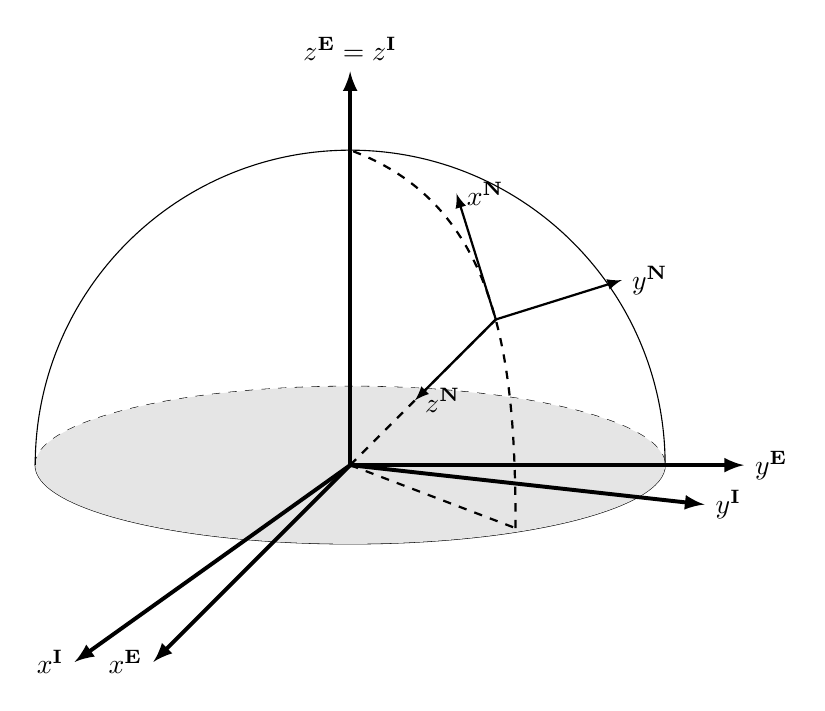
\begin{tikzpicture}
			        % base circle
			        \draw (-4,0) arc (180:360:4 and 1);
			        \draw [dashed] (-4,0) arc (180:0:4 and 1);

			        % fill
			        \filldraw[fill=gray!20, draw=none] (-4,0) arc (180:360:4 and 1) -- (4,0) arc (0:180:4 and 1) -- cycle;


			        % Circle around the plate border
			        \draw (-4,0) arc (180:0:4 and 4);


			        % Draw the lines
			        \draw [thick, ->, line width=.5mm] (0,0) -- ++(-2.5,-2.5) node [left] {$x^{\mathbf{E}}$};
					\draw [thick, ->, line width=.5mm] (0,0) -- ++(-2.5-1,-2.5) node [left] {$x^{\mathbf{I}}$};
			        \draw [thick, ->, line width=.5mm] (0,0) -- ++(0,5) node [above] {$z^{\mathbf{E}}=z^{\mathbf{I}}$};
			        \draw [thick, ->, line width=.5mm] (0,0) -- ++ (5,0) node [right] {$y^{\mathbf{E}}$};
					\draw [thick, ->, line width=.5mm] (0,0) -- ++ (4.5,-0.5) node [right] {$y^{\mathbf{I}}$};


			        % define coordinate
			        \coordinate (A) at (2.1,-.8);
			        % Draw the dashed line from center to plate border
			        \draw [thick, dashed] (0,0) -- ++ (A);

			        % Draw the arc from the top of the circle to the dashed line
			        % \tikz[every to/.style={bend left}]
			        \draw [thick, dashed] (2.1,-.8) to
			        [out=90,in=-20]
			        (0,4);


			        \coordinate (B) at (1.85,1.85);

			        \draw [thick, dashed] (0,0) -- ++ (B);

			        % Navigation coordinate system
			        % x axis
			        \draw [thick, ->] (B) -- ++ (-.5, 1.6) node [right] {$x^{\mathbf{N}}$};
			        % y axis
			        \draw [thick, ->] (B) -- ++ (1.6, .5) node [right] {$y^{\mathbf{N}}$};
			        % z axis
			        \draw [thick, ->] (B) -- ++ (-1.85/1.8, -1.85/1.8) node [right] {$z^{\mathbf{N}}$};
			    \end{tikzpicture}
			      }\label{fig:navigation}}
	\\
	\hspace{-3cm}
	\subfloat[]{
		\resizebox{.8\textwidth}{!}{
    \begin{tikzpicture}
        % Add horizontal space before the image to shift it to the right
         % Adjust this value to move the image horizontally
        \begin{scope}
            \node[anchor=south west,inner sep=0] (image) at (0,0) {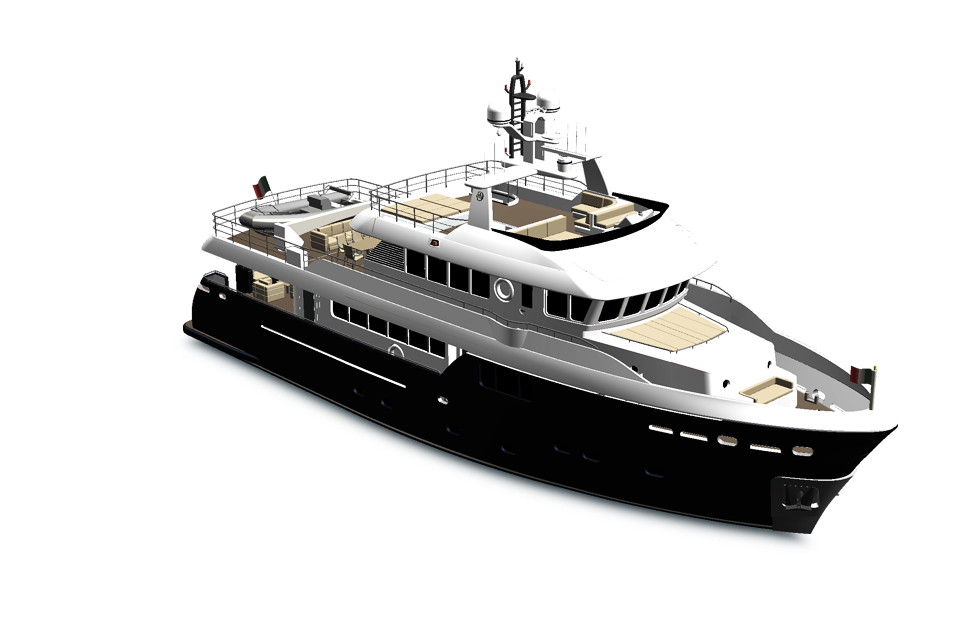
\includegraphics[width=1.5\textwidth]{../Figure/ship.png}};
            \begin{scope}[x={(image.south east)},y={(image.north west)}]
            % add center of mass
            \node at (image.center) {\centerofmass};
            % add x axis
            \draw[->, line width=0.5mm] (image.center) -- ++(0.5,-0.22) node [right] {\Huge $x^{\mathbf{M}}$};
            % add y axis
            \draw[->, line width=0.5mm] (image.center) -- ++(-0.3,-0.3) node [below] {\Huge $y^{\mathbf{M}}$};
            % add z axis
            \draw[->, line width=0.5mm] (image.center) -- ++(0,-0.4) node [below] {\Huge $z^{\mathbf{M}}$};
            \end{scope}
        \end{scope}
    \end{tikzpicture}%
}\label{fig:master}}
	\hspace{-1cm}
	\subfloat[]{
		% \hspace{-4cm}
		\resizebox{0.3\textwidth}{!}{
		\begin{tikzpicture}
	        \begin{scope}
	            \node[anchor=south west,inner sep=0] (image) at (0,0) {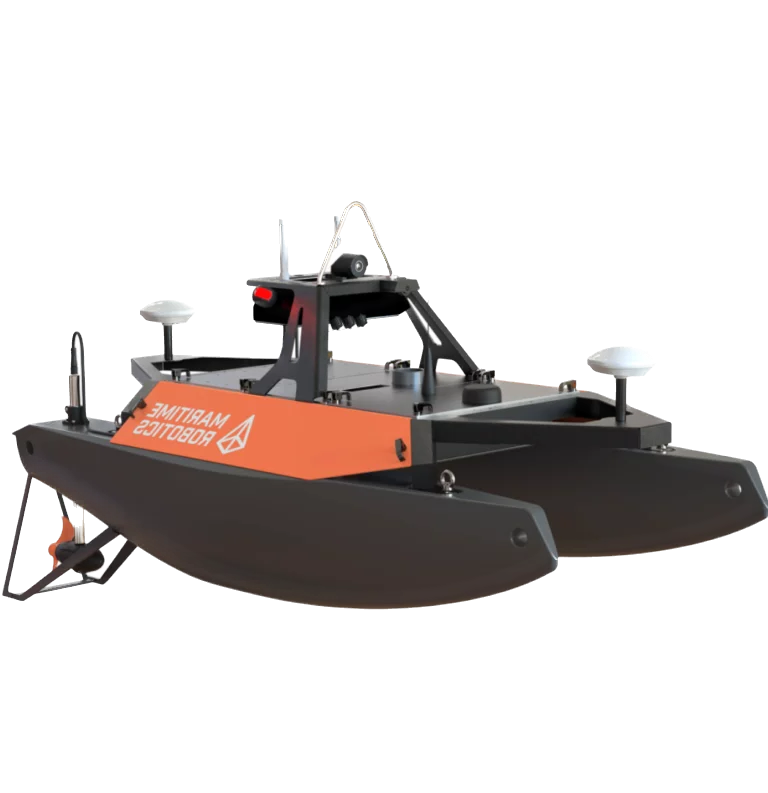
\includegraphics[width=0.7\textwidth]{../Figure/otter.png}};
	            \begin{scope}[x={(image.south east)},y={(image.north west)}]
	            % add center of mass
	            \node at (image.center) {\centerofmass};
	            % add x axis
	            \draw[->, line width=0.5mm] (image.center) -- ++
	            (0.5,-0.07) node [right] {\Huge $x^{\mathbf{S}}$};
	            % add y axis
	            \draw[->, line width=0.5mm] (image.center) -- ++
	            (-0.4*1.5,-0.1*1.5) node [below] {\Huge $y^{\mathbf{S}}$};
	            % add z axis
	            \draw[->, line width=0.5mm] (image.center) -- ++
	            (0,-0.4) node [below] {\Huge $z^{\mathbf{S}}$};
	            % center of mass text
	            % \node at (image.center) [
	            % yshift=1.5cm, xshift=1.5cm]
	            % {Center of Mass};
	            \end{scope}
	        \end{scope}
	    \end{tikzpicture}%
		}\label{fig:slave_otter}}

	\caption{Graphical Representation of the Presented Reference Frames:~\ref{sub@fig:navigation} Inertial, Earth, and Navigation Frames~\ref{sub@fig:master}~Master Frame~\ref{sub@fig:slave_otter} Slave Frame
	}\label{fig:frames}
\end{figure}





% \begin{figure}
%     \centering
%     \begin{subfigure}{.5\textwidth}
%       \centering
%       {
%       \begin{tikzpicture}
%         % base circle
%         \draw (-4,0) arc (180:360:4 and 1);
%         \draw [dashed] (-4,0) arc (180:0:4 and 1);

%         % fill
%         \filldraw[fill=gray!20, draw=none] (-4,0) arc (180:360:4 and 1) -- (4,0) arc (0:180:4 and 1) -- cycle;


%         % Circle around the plate border
%         \draw (-4,0) arc (180:0:4 and 4);


%         % Draw the lines
%         \draw [thick, ->, line width=.5mm] (0,0) -- ++(-2.5,-2.5) node [left] {$x^{\mathbf{E}}$};
%         \draw [thick, ->, line width=.5mm] (0,0) -- ++(0,5) node [above] {$y^{\mathbf{E}}$};
%         \draw [thick, ->, line width=.5mm] (0,0) -- ++ (5,0) node [right] {$z^{\mathbf{E}}$};


%         % define coordinate
%         \coordinate (A) at (2.1,-.8);
%         % Draw the dashed line from center to plate border
%         \draw [thick, dashed] (0,0) -- ++ (A);

%         % Draw the arc from the top of the circle to the dashed line
%         % \tikz[every to/.style={bend left}]
%         \draw [thick, dashed] (2.1,-.8) to
%         [out=90,in=-20]
%         (0,4);


%         \coordinate (B) at (1.85,1.85);

%         \draw [thick, dashed] (0,0) -- ++ (B);

%         % Navigation coordinate system
%         % x axis
%         \draw [thick, ->] (B) -- ++ (-.5, 1.6) node [right] {$x^{\mathbf{N}}$};
%         % y axis
%         \draw [thick, ->] (B) -- ++ (1.6, .5) node [right] {$y^{\mathbf{N}}$};
%         % z axis
%         \draw [thick, ->] (B) -- ++ (-1.85/1.8, -1.85/1.8) node [right] {$z^{\mathbf{N}}$};
%     \end{tikzpicture}
%       }

%       \caption{Navigation and Earth Frame}
%       \label{fig:navigation}
%     \end{subfigure}%
%     \begin{subfigure}{.5\textwidth}
%       \centering
%       {
%       \begin{tikzpicture}
%         \begin{scope}[xshift=1.5cm]
%             \node[anchor=south west,inner sep=0] (image) at (0,0) {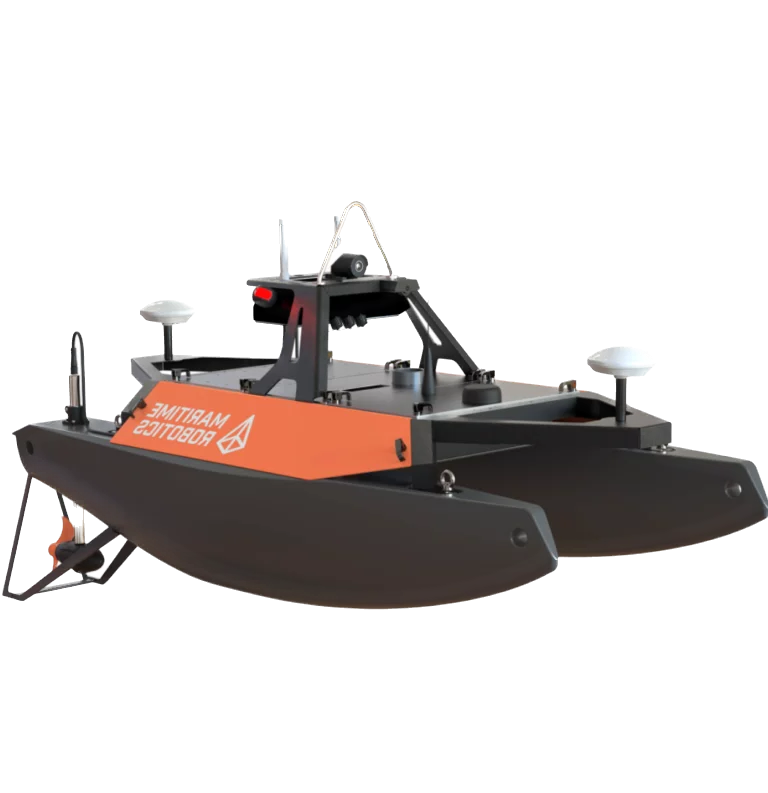
\includegraphics[width=0.7\textwidth]{../Figure/otter.png}};
%             \begin{scope}[x={(image.south east)},y={(image.north west)}]
%             % add center of mass
%             \node at (image.center) {\centerofmass};
%             % add x axis
%             \draw[->, line width=0.5mm] (image.center) -- ++
%             (0.5,-0.07) node [right] {$x^{\mathbf{S}}$};
%             % add y axis
%             \draw[->, line width=0.5mm] (image.center) -- ++
%             (-0.4,-0.1) node [below] {$y^{\mathbf{S}}$};
%             % add z axis
%             \draw[->, line width=0.5mm] (image.center) -- ++
%             (0,-0.4) node [below] {$z^{\mathbf{S}}$};
%             % center of mass text
%             % \node at (image.center) [
%             % yshift=1.5cm, xshift=1.5cm]
%             % {Center of Mass};
%             \end{scope}
%         \end{scope}
%     \end{tikzpicture}%
%       }
%       \caption{Slave Reference Frame}
%       \label{fig:slave}
%     \end{subfigure}
%     \caption{Graphical Representation of the Presented Reference Frames}
%     \label{fig:frames}
%     \end{figure}

% \begin{figure}
%     \centering
%     \begin{subfigure}{.5\textwidth}
%         \centering
%         \begin{tikzpicture}
%             % base circle
%             \draw (-4,0) arc (180:360:4 and 1);
%             \draw [dashed] (-4,0) arc (180:0:4 and 1);

%             % fill
%             \filldraw[fill=gray!20, draw=none] (-4,0) arc (180:360:4 and 1) -- (4,0) arc (0:180:4 and 1) -- cycle;

%             % Circle around the plate border
%             \draw (-4,0) arc (180:0:4 and 4);

%             % Draw the lines
%             \draw [thick, ->, line width=.5mm] (0,0) -- ++(-2.5,-2.5) node [left] {$x^{\mathbf{E}}$};
%             \draw [thick, ->, line width=.5mm] (0,0) -- ++(0,5) node [above] {$y^{\mathbf{E}}$};
%             \draw [thick, ->, line width=.5mm] (0,0) -- ++ (5,0) node [right] {$z^{\mathbf{E}}$};

%             % define coordinate
%             \coordinate (A) at (2.1,-.8);
%             % Draw the dashed line from center to plate border
%             \draw [thick, dashed] (0,0) -- ++ (A);

%             % Draw the arc from the top of the circle to the dashed line
%             \draw [thick, dashed] (2.1,-.8) to [out=90,in=-20] (0,4);

%             \coordinate (B) at (1.85,1.85);
%             \draw [thick, dashed] (0,0) -- ++ (B);

%             % Navigation coordinate system
%             % x axis
%             \draw [thick, ->] (B) -- ++ (-.5, 1.6) node [right] {$x^{\mathbf{N}}$};
%             % y axis
%             \draw [thick, ->] (B) -- ++ (1.6, .5) node [right] {$y^{\mathbf{N}}$};
%             % z axis
%             \draw [thick, ->] (B) -- ++ (-1.85/1.8, -1.85/1.8) node [right] {$z^{\mathbf{N}}$};
%         \end{tikzpicture}
%         \caption{Navigation and Earth Frame}
%         \label{fig:navigation}
%     \end{subfigure}%
%     \begin{subfigure}{.5\textwidth}
%         \centering
%         \begin{tikzpicture}
%             \node[anchor=south west,inner sep=0] (image) at (0,0) {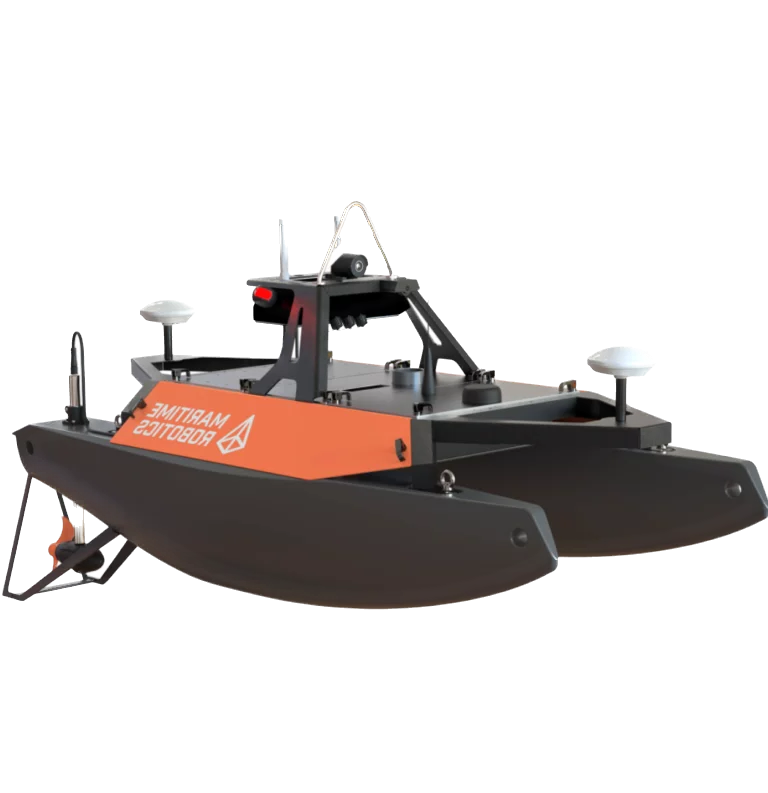
\includegraphics[width=0.7\textwidth]{../Figure/otter.png}};
%             \begin{scope}[x={(image.south east)},y={(image.north west)}]
%                 % add center of mass
%                 \node at (0.5,0.5) {\(\bullet\)};
%                 % add x axis
%                 \draw[->, line width=0.5mm] (0.5,0.5) -- ++ (0.5,-0.07) node [right] {$x^{\mathbf{S}}$};
%                 % add y axis
%                 \draw[->, line width=0.5mm] (0.5,0.5) -- ++ (-0.4,-0.1) node [below] {$y^{\mathbf{S}}$};
%                 % add z axis
%                 \draw[->, line width=0.5mm] (0.5,0.5) -- ++ (0,-0.4) node [below] {$z^{\mathbf{S}}$};
%             \end{scope}
%         \end{tikzpicture}
%         \caption{Slave Reference Frame}
%         \label{fig:slave}
%     \end{subfigure}
%     \caption{Graphical Representation of the Presented Reference Frames}
%     \label{fig:frame}
% \end{figure}






\section{Modeling}\label{sec:model}
\noindent In this section, the measurements, provided by the GPS receiver and the IMU of the USV and AUV, are modeled.
\subsection{Inertial Measurement Unit}
\noindent The specific force,
\({{\left[\tilde{{\mathbf{f}}}_{\mathbf{BI}}\right]}}^{\mathbf{B}}\),
and the angular rate of the \(\mathbf{B}\) frame with respect to \(\mathbf{I}\) frame, \({\left[\tilde{\boldsymbol{\omega}}_{\mathbf{BI}}\right]}^{\mathbf{B}}\), are measured by the accelerometer and the gyroscope, respectively. Therefore, the IMU outputs of the master and slave vehicles
(for \(\mathbf{B} = \mathbf{M} \text{ \& } \mathbf{S}\))
are modeled as follows:
\begin{align}
	{{\left[\tilde{\mathbf{f}}_{\mathbf{BI}}\right]}}^{\mathbf{B}} =& {\left[\mathbf{f}_{\mathbf{BI}}\right]}^{\mathbf{B}} + {{\left[\mathbf{b}_{{a}}\right]}}^{\mathbf{B}} +\boldsymbol{\eta}_{{a}}, \\
	{{\left[\tilde{\boldsymbol{\omega}}_{\mathbf{BI}}\right]}}^{\mathbf{B}} =& {{\left[\boldsymbol{\omega}_{\mathbf{BI}}\right]}}^{\mathbf{B}} + {{\left[\mathbf{b}_{{g}}\right]}}^{\mathbf{B}} +\boldsymbol{\eta}_{{g}},
\end{align}
where \({{\left[\mathbf{f}_{\mathbf{BI}}\right]}}^{\mathbf{B}} = \begin{bmatrix}
	f_x & f_y & f_z
\end{bmatrix}^{\mathrm{T}}\) and \({{\left[\boldsymbol{\omega}_{\mathbf{BI}}\right]}}^{\mathbf{B}} = \begin{bmatrix}
	\omega_x & \omega_y & \omega_z
	\end{bmatrix}^{\mathrm{T}}\) are, respectively, the true values of accelerometer and gyroscope sensors. The \({\left[\mathbf{b}_{a}\right]}^{\mathbf{B}} = \begin{bmatrix}
		{b}_{a_{x}} & {b}_{a_{y}} & {b}_{a_{z}}
	\end{bmatrix}^{\mathrm{T}}\) and \({\left[\mathbf{b}_{g}\right]}^{\mathbf{B}} = \begin{bmatrix}
		{b}_{g_{x}} & {b}_{g_{y}} & {b}_{g_{z}}
	\end{bmatrix}^{\mathrm{T}}\) are modeled as random constants, that vary from run-to-run,  as follows:
	\begin{align}
		\dot{\mathbf{b}}_{a} &= \mathbf{0}, \\
		\dot{\mathbf{b}}_{g} &= \mathbf{0}.
	\end{align}
	Moreover, \(\boldsymbol{\eta}_{{a}}\) and \(\boldsymbol{\eta}_{{g}}\) are the Gaussian white noise of measurements.

\subsection{GPS Modeling}
\noindent A GPS receiver of the master vehicle measures the velocity and position vectors at 1 Hz rate. It is assumed that these measurements are computed as
\begin{align}
    \label{eq:gps_meas1}
    {\left[\tilde{{\mathbf{v}}}_{\mathbf{M}}\right]}^{\mathbf{N}} &= {\left[{\mathbf{v}}_{\mathbf{M}}\right]}^{\mathbf{N}} + \boldsymbol{\eta}_{v_{\mathbf{M}}}, \\
    \label{eq:gps_meas2}
    \tilde{{\mathbf{p}}}_{\mathbf{M}} &= {\mathbf{p}_{\mathbf{M}}} + \boldsymbol{\eta}_{p_{\mathbf{M}}},
\end{align}
where, \({\left[\mathbf{v}_{\mathbf{M}}\right]}^{\mathbf{N}} = \begin{bmatrix}
	v_n & v_e & v_d
	\end{bmatrix}^{\mathrm{T}}\) is the ground velocity of the master vehicle denoted in the \({\mathbf{N}}\) frame and \(\mathbf{p}_{\mathbf{M}} = \begin{bmatrix}
		L & \lambda & h
		\end{bmatrix}^{\mathrm{T}}\) is the position vector that represents the  lateral, longitudinal and height of the master vehicle. Moreover, \(\boldsymbol{\eta}_{v_{\mathbf{M}}}\) and \(\boldsymbol{\eta}_{p_{\mathbf{M}}}\) denote the measurement noises of the GPS, modeled as Gaussian white noise.

\section{SINS Mechanization}\label{sec:SINS}
\noindent Here, the nonlinear equations of motion of the SINS are utilized to describe the kinematic of the vehicle including the attitude, velocity, and position. These equations are denoted as~\cite{bekir2007introduction}:
%\newpage
%%\begin{strip}
\begin{align}
\centering
		\label{eq:INS1}
		\dot{\mathbf{C}}_{\mathbf{B}_{\text{SINS}}}^{\mathbf{N}} &=
		{\left[\boldsymbol{{\omega}}_{\mathbf{NI}_{\mathbf{B}_{\text{SINS}}}}\right]}^{\mathbf{N}}  \times \mathbf{C}_{\mathbf{B}_{\text{SINS}}}^{\mathbf{N}}
		- \mathbf{C}_{\mathbf{B}_{\text{SINS}}}^{\mathbf{N}} {\left[\boldsymbol{\tilde{\omega}}_{\mathbf{BI}}\right]}^{\mathbf{B}}, \\
		\label{eq:INS2}
		{{\left[{{\dot{\mathbf{v}}}}_{{\mathbf{B}_{\text{SINS}}}}\right]}^{\mathbf{N}}} &= {\mathbf{C}}_{\mathbf{B}_{\text{SINS}}}^{\mathbf{N}}{\left[\tilde{\mathbf{{f}}}_{\mathbf{BI}}\right]}^{\mathbf{B}} - \left( 2{{\left[\boldsymbol{\omega}_{{\mathbf{EI}}_{\mathbf{B}_{\text{SINS}}}}\right]}^{\mathbf{N}} + {\left[\boldsymbol{\omega}_{{\mathbf{NE}}_{\mathbf{B}_{\text{SINS}}}}\right]}^{\mathbf{N}}} \right)\times{{{\left[\mathbf{v}_{\mathbf{B}_{\text{SINS}}}\right]}}^{\mathbf{N}}} + {{\left[{\mathbf{g}}_{{\text{eff}}_{\mathbf{B}_{\text{SINS}}}}\right]}^{\mathbf{N}}},\\
		\label{eq:INS3}
		\dot{\mathbf{p}}_{\mathbf{B}_{\text{SINS}}} &= \begin{bmatrix}
			\dot{L} \\
			\dot{\lambda} \\
			\dot{h}
		\end{bmatrix} = \begin{bmatrix}
			\dfrac{v_n}{\mathrm{R_N}+h}\\[1em]
			\dfrac{v_e}{(\mathrm{R_E} + h)\cos(L)}\\
			-v_d
		\end{bmatrix},
	\end{align}
%%\end{strip}
%\begin{figure}
%\end{figure}
where \(\mathbf{B} = \mathbf{M} \text{ \& } \mathbf{S}\)
is related to the master and slave vehicles, respectively. The
 notation \(\times\) denotes the cross product operator and \(\mathbf{C}_{\mathbf{B}}^{\mathbf{N}}\) is the Direction Cosine Matrix (DCM), transforming the \({\mathbf{B}}\) frame to \({\mathbf{N}}\) frame.
	Moreover, \({\left[{\boldsymbol{\omega}}_{\mathrm{NI}}\right]}^{\mathbf{N}}\) is the angular velocity of
the \({\mathbf{N}}\) frame with respect to \({\mathbf{I}}\) frame, denoted in \({\mathbf{N}}\) frame, modeled as
\begin{equation}
{\left[{\boldsymbol{\omega}}_{\mathbf{NI}_{\mathbf{B}_{\text{SINS}}}}\right]}^{\mathbf{N}} = {\left[{\boldsymbol{\omega}}_{\mathbf{NE}_{\mathbf{B}_{\text{SINS}}}}\right]}^{\mathbf{N}} + {\left[{\boldsymbol{\omega}}_{\mathbf{EI}_{\mathbf{B}_{\text{SINS}}}}\right]}^{\mathbf{N}},
\end{equation}
where, \({\left[{\boldsymbol{\omega}}_{\mathbf{NE}_{\mathbf{B}}}\right]}^{\mathbf{N}}\) is the transport rate, denoted in N frame, modeled as
\begin{equation}
	{\left[{\boldsymbol{\omega}}_{{\mathbf{NE}}_{\mathbf{B}_{\text{SINS}}}}\right]}^{\mathbf{N}} = \begin{bmatrix}
		\dfrac{v_e}{\mathrm{R_E} + h}\\[1em]
		\dfrac{-v_n}{\mathrm{R_N} + h} \\[1em]
		\dfrac{-v_e\tan(L)}{\mathrm{R_E} + h}
	\end{bmatrix},
\end{equation}
and
\({\left[{\boldsymbol{\omega}}_{\mathrm{EI}_{\mathbf{B}}}\right]}^{\mathbf{N}} \) is the earth rate, denoted in \({\mathbf{N}}\) frame, defined as
\begin{equation}
	{\left[{\boldsymbol{\omega}}_{{\mathbf{EI}}_{\mathbf{B}_{\text{SINS}}}}\right]}^{\mathbf{N}} = \begin{bmatrix}
		{{\Omega}}\cos {{L}} \\
		0 \\
		-{\Omega}\sin {{L}}
	\end{bmatrix}.
\end{equation}
% \({\left[\mathbf{{\Omega}}_{\mathbf{EI}}\right]}^{\mathbf{N}}\)
% and
% \({\left[\mathbf{{\Omega}}_{\mathbf{NE}}\right]}^{\mathbf{N}}\)
% are the skew-symmetric forms of the vectors \({\left[
% 	\mathbf{{\omega}}_{\mathbf{EI}}\right]}^{\mathbf{N}}\) and \({\left[
% 		\mathbf{{\omega}}_{\mathbf{NE}}\right]}^{\mathbf{N}}\), respectively.
Here, \(\mathrm{R_N}\) and \(\mathrm{R_E}\) are, respectively, the meridional and the transverse radius of the curvature, defined as
\begin{equation}
	\mathrm{R_N} = \dfrac{\mathrm{R_0}(1-\mathrm{e}^2)}{{(1-\mathrm{e}^2\sin^2(L))}^{\frac{3}{2}}},
\end{equation}
\begin{equation}
	\mathrm{R_E} = \dfrac{\mathrm{R_0}}{{(1-\mathrm{e}^2\sin^2(L))}^{\frac{1}{2}}},
\end{equation}
where \(\mathrm{R_0}\) and \(\mathrm{e}\) are the equatorial radius and the eccentricity of the Earth ellipsoid. Finally, the term \({\left[\mathbf{g}_{\mathrm{eff}}\right]}^{\mathbf{N}}\) is the effective gravity, denoted in the \({\mathbf{N}}\) frame, represented as~\cite{groves2013principles}:
\begin{equation}
	{\left[\mathbf{g}_{\mathrm{eff}_{\mathbf{B}_{\text{SINS}}}}\right]}^{\mathbf{N}} = \begin{bmatrix}
		0 \\
		0 \\
		\mathrm{g_0}\dfrac{\mathrm{R}_{\mathrm{G}}^2}{{(\mathrm{R_G}+h)}^2}
	\end{bmatrix},
\end{equation}
where \(\mathrm{R_G} = \sqrt{\mathrm{R_N}\mathrm{R_E}} \) is the Gaussian radius and term \(\mathrm{g_0}\) is calculated as
\begin{align*}
	\mathrm{g_{\rm{0}}} =\; &9.780318(1 + 5.3024 \times {10^{ - 3}}{\sin ^2}(L)  \\
	- &5.9 \times {10^{ - 6}}{\sin ^2}(2L)).
\end{align*}




\section{Structure of the Master Navigation}\label{sec:master}
\noindent The structure of the master navigation unit is shown in Fig~\ref{fig:master_struct}, when the GPS signal is available. The computer of the master vehicle is equipped with a SINS based on the inertial sensors, including a gyroscope and an accelerometer, as well as a GPS receiver to provide information such as position (\(\mathbf{p_M}\)), velocity (\(\mathbf{v_M}\)), and attitude (\(\mathbf{a_M}\)). Then, the difference between the velocities of the GPS and SINS is utilized in the closed loop KF to estimate the errors of the position, velocity, and attitude. The estimated errors are computed in the structure of the master SINS at each sample time.

\begin{figure}[h]
	\centering
	\resizebox{.8\textwidth}{!}{
        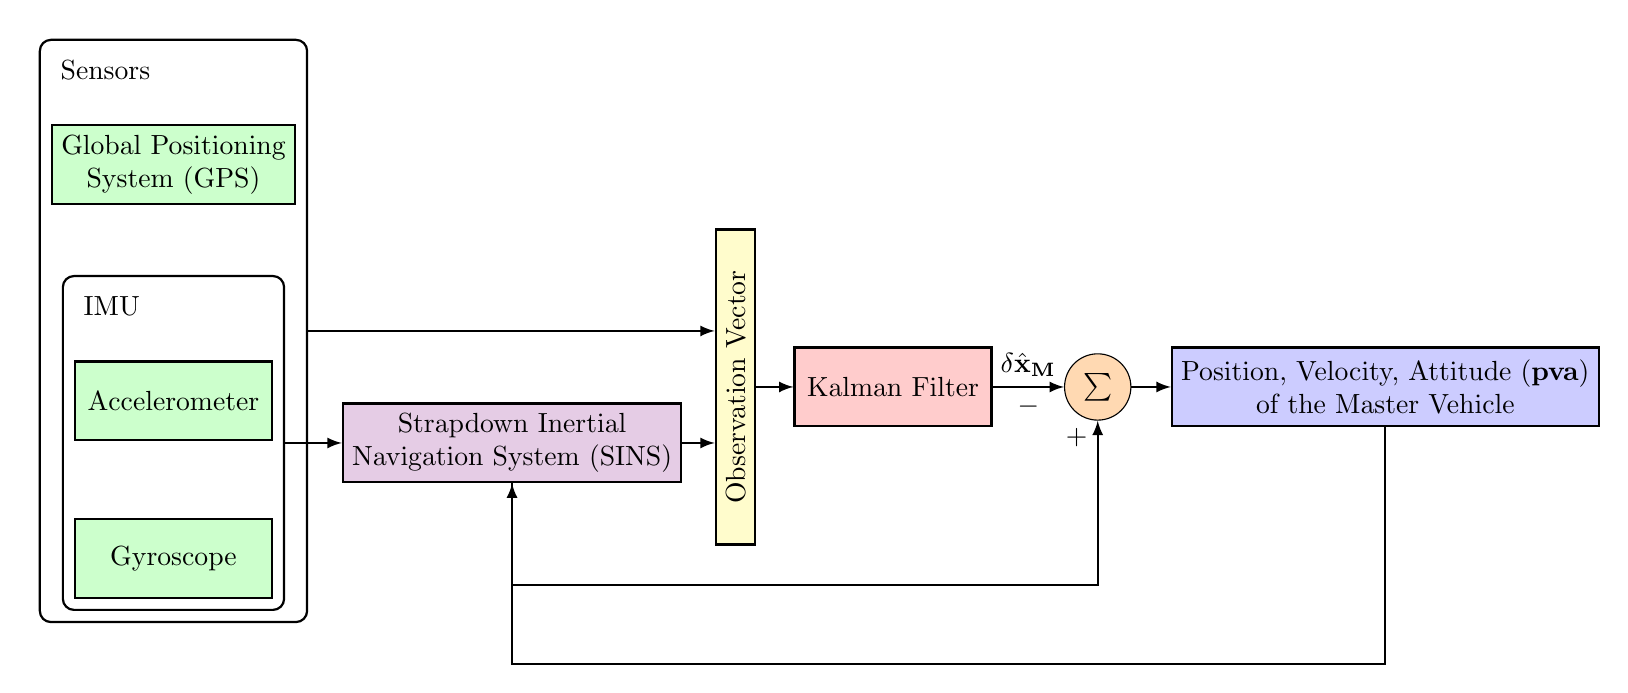
\begin{tikzpicture}
            % Draw the first inner rectangle (below) with start label
            \node[sensor] (Gyroscope) at (3, 3) {Gyroscope};

            % Draw the second inner rectangle (above) with stop label
            \node[sensor] (Accelerometer) at (3, 5) {Accelerometer};

            % Draw the IMU label above and aligned with Accelerometer
            \node[above=1.2cm of Accelerometer.west, anchor=west] (IMU) {IMU};

            % Draw the outer rectangle tightly around the two inner rectangles
            \node[draw, thick, fit=(Accelerometer) (Gyroscope) (IMU), inner sep=4pt, rounded corners] (IMU_outer) {};

            \node[sensor, align=center] (GPS) at (3, 8) {Global Positioning\\ System (GPS)};

            % draw outer label for IMU_outer and GPS
            \node[above=1.2cm of GPS.west, anchor=west] (sensor_diag) {Sensors};

            % Draw the outer rectangle tightly around the two inner rectangles
            \node[draw, thick, fit=(IMU_outer) (GPS) (sensor_diag), inner sep=4pt, rounded corners] (sensor_outer) {};

            % SINS
            \node[sensor, align=center, fill=violet!20, right of=IMU_outer, xshift=3.3cm]
             (SINS)
              {Strapdown Inertial\\ Navigation System (SINS)};

            % group SINS and Sensors
            \node[draw=none, thick, fit=(SINS) (sensor_outer), inner sep=4pt] (system) {};

            % observation vector
            \node[observation] at ($(system)!0.5!(SINS)$) [xshift=3.8cm]
             (observation)
             {\rotatebox{90}{Observation Vector}};

            % Kalman Filter
            \node[kf, right of=observation, xshift=1cm]
             (KF)
              {Kalman Filter};

            % plot circle right of KF to show summation
            \node[draw, circle,fill=orange!30, right of=KF, xshift=1.6cm] (sum)
            % add sum symbol
            {$\sum$};
            \coordinate[below=.5cm of observation] (bottom);
            % add PVA
            \node[pva, right =of sum.east, xshift=-0.5cm, align=center] (PVA) {Position, Velocity, Attitude (\(\mathbf{pva}\))\\ of the Master Vehicle};



            % connect IMU_outer and SINS
            \draw[->, thick] (IMU_outer) -- (SINS);
            % connect Sensors and SINS to observation
            \draw[->, thick] (SINS.east) -- (observation.west |- SINS);
            \draw[->, thick] (sensor_outer.east) -- (observation.west |- sensor_outer);
            % connect observation to KF
            \draw[->, thick] (observation) -- (KF);
            % connect KF to sum and write - on line
            \draw[->, thick] (KF) -- (sum) node[midway, above] {$\delta \hat{\mathbf{x}}_{\mathbf{M}}$}
            node[midway, below] {$-$};
            % connect SINS to sum from below add + at the end of line
            \draw[->, thick] (SINS.south) |- (bottom) -| (sum)
            node[pos=.95, left] {$+$};
            % connect sum to PVA
            \draw[->, thick] (sum) -- (PVA);
            % connect PVA to SINS
            \draw[->, thick] (PVA.south) |- ($(bottom) + (0,-1cm)$) -| (SINS);

        \end{tikzpicture}
    }
	\caption{Structure of Integrated Navigation of the Master Vehicle}\label{fig:master_struct}
\end{figure}



The GPS receiver of the master navigation unit is depended on the signals, transmitted from the satellites. Therefore, the integrated navigation of the master vehicle can be distributed, when the GPS signals outage. To solve this problem, the Neural Network (NN) method,
obtained from two stages:
training and prediction.
For this purpose, first, the proposed NN is trained based on the results of the integrated navigation of the master vehicle in the presence of the GPS data. Then, the prediction stage of the proposed NN is performed to provide the required information of the master vehicle. The structure of the integrated navigation unit of the master vehicle is shown in Fig~\ref{fig:master_struct_gps_outage}, when the GPS outages. In the following, the details of the navigation structure of the master vehicle are denoted.




\begin{figure}[h]
	\centering
	\resizebox{1\textwidth}{!}{
        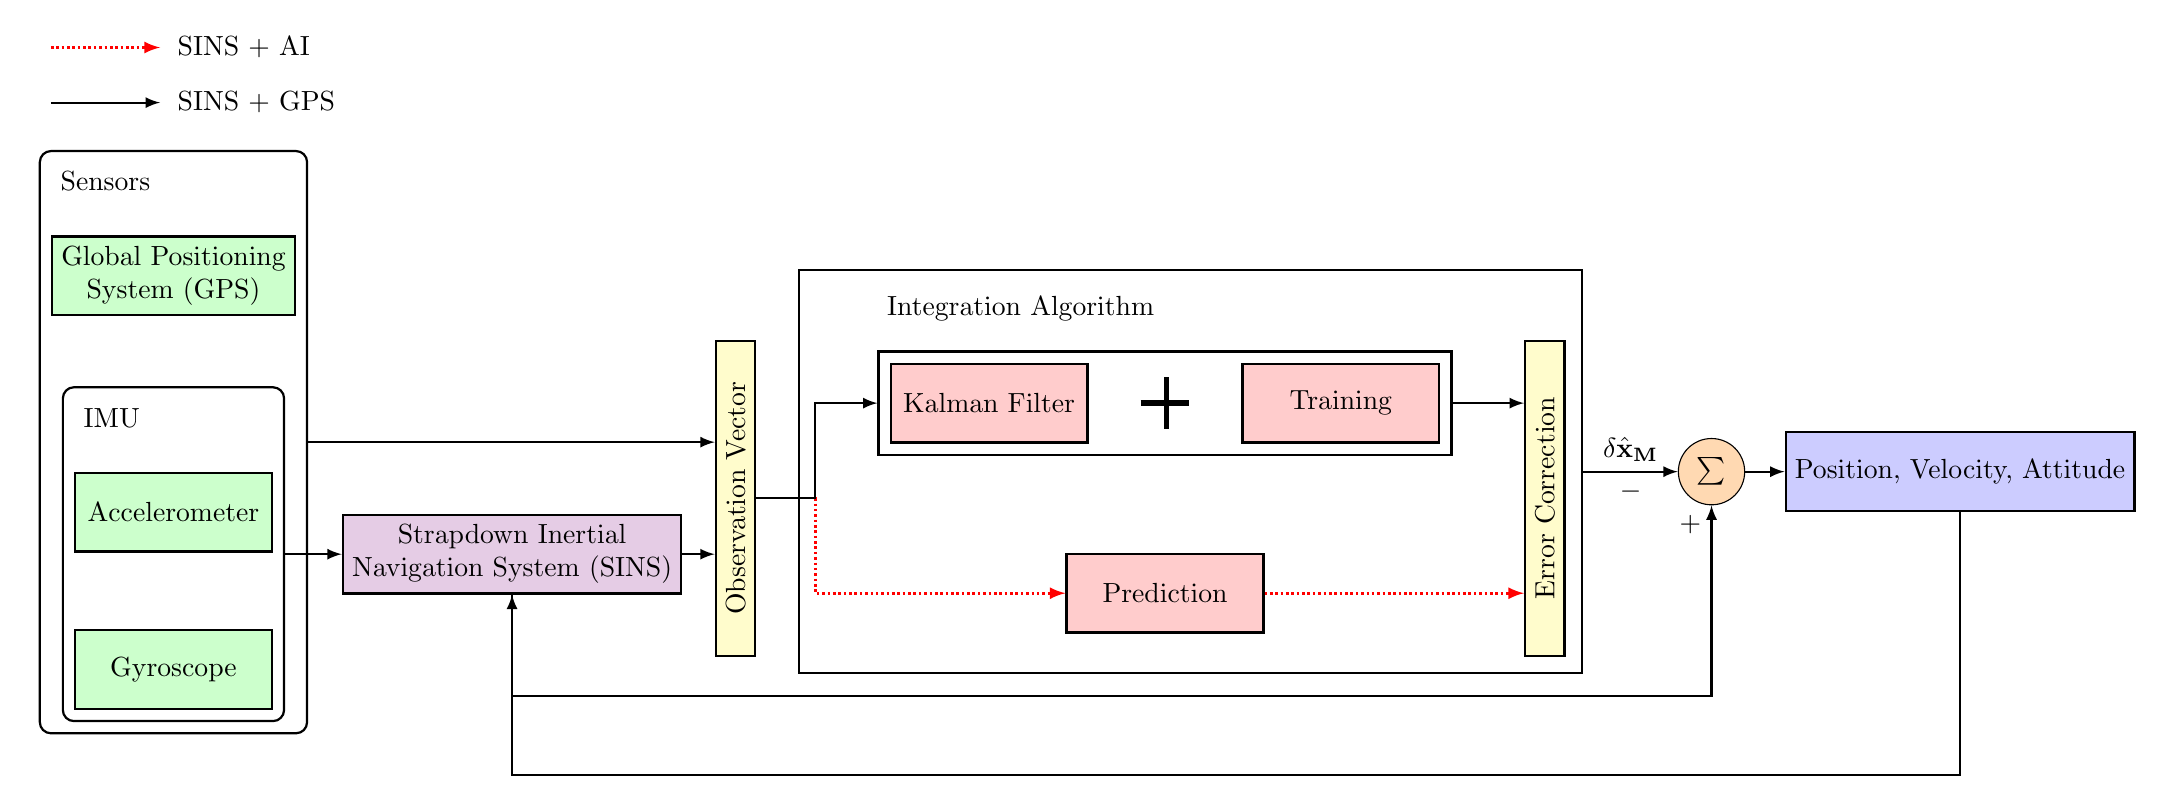
\begin{tikzpicture}
            % Draw the first inner rectangle (below) with start label
            \node[sensor] (Gyroscope) at (3, 3) {Gyroscope};

            % Draw the second inner rectangle (above) with stop label
            \node[sensor] (Accelerometer) at (3, 5) {Accelerometer};

            % Draw the IMU label above and aligned with Accelerometer
            \node[above=1.2cm of Accelerometer.west, anchor=west] (IMU) {IMU};

            % Draw the outer rectangle tightly around the two inner rectangles
            \node[draw, thick, fit=(Accelerometer) (Gyroscope) (IMU), inner sep=4pt, rounded corners] (IMU_outer) {};

            \node[sensor, align=center] (GPS) at (3, 8) {Global Positioning\\ System (GPS)};

            % draw outer label for IMU_outer and GPS
            \node[above=1.2cm of GPS.west, anchor=west] (sensor_diag) {Sensors};

            % Draw the outer rectangle tightly around the two inner rectangles
            \node[draw, thick, fit=(IMU_outer) (GPS) (sensor_diag), inner sep=4pt, rounded corners] (sensor_outer) {};

            % SINS
            \node[sensor, align=center, fill=violet!20, right of=IMU_outer, xshift=3.3cm]
             (SINS)
              {Strapdown Inertial\\ Navigation System (SINS)};

            % group SINS and Sensors
            \node[draw=none, thick, fit=(SINS) (sensor_outer), inner sep=4pt] (system) {};

            % observation vector
            \node[observation] at ($(system)!0.5!(SINS)$) [xshift=3.8cm]
             (observation)
             {\rotatebox{90}{Observation Vector}};

             \coordinate[right=.75cm of observation] (connections);




            % Kalman Filter
            \node[kf, above right of=connections, xshift=1.5cm, yshift=.5cm]
             (KF)
              {Kalman Filter};

            % add plus sign
            \node[right=0.5cm of KF] (plus) {\fplus[black]};

            % add training phase
            \node[kf, right=0.5cm of plus] (training) {Training};


            % box to fit KF and training
            \node[draw, thick, fit=(KF) (training), inner sep=4pt] (KF_outer) {};


             % Calculate the horizontal midpoint between KF and training
            \coordinate (midpoint) at ($(KF)!0.5!(training)$);

            % Calculate the y-distance between connections and KF
            \path let \p1 = (connections), \p2 = (KF) in
            coordinate (prediction_pos) at (\x1, \y1 - \y2 + \y1);

            % Prediction node, ensuring symmetry
            \node[kf, at={(midpoint |- prediction_pos)}] (prediction) {Prediction};

            % error correction
            \node[observation, right=9cm of connections] (error)
            {\rotatebox{90}{Error Correction}};

            % add label for KF_outer
            \node[above=1.2cm of KF_outer.west, anchor=west] (Integration) {Integration Algorithm};

            % add outer box for error correction, prediction, and KF
            \node[draw, thick, fit=(error) (prediction) (KF_outer)
            (connections) (Integration)
            , inner sep=6pt] (error_outer) {};





            % % plot circle right of KF to show summation
            \node[draw, circle,fill=orange!30, right=-.cm of error_outer.east, xshift=1.2cm] (sum)
            % add sum symbol
            {$\sum$};
            \coordinate[below=.5cm of observation] (bottom);
            % add PVA
            \node[pva, right =of sum.east, xshift=-0.5cm] (PVA) {Position, Velocity, Attitude};



            % connect IMU_outer and SINS
            \draw[->, thick] (IMU_outer) -- (SINS);
            % connect Sensors and SINS to observation
            \draw[->, thick] (SINS.east) -- (observation.west |- SINS);
            \draw[->, thick] (sensor_outer.east) -- (observation.west |- sensor_outer);
            % connect observation to prediction with red .... line
            \draw[->, densely dotted, line width=0.33mm, red] (observation) -| (connections) |- (prediction);
            % connect observation to KF
            \draw[->, thick] (observation) -| (connections) |- (KF_outer);
            % connect KF outer to error correction
            \draw[->, thick] (KF_outer.east) -- (error.west |- KF_outer.east);
            % connect prediction to error correction
            \draw[->, densely dotted, line width=0.33mm, red] (prediction) -- (error.west |- prediction);
            % % connect observation to KF
            % \draw[->, thick] (observation) -- (KF);
            % % connect KF to sum and write - on line
            \draw[->, thick] (error_outer) -- (sum) node[midway, above] {$\delta \hat{\mathbf{x}}_{\mathbf{M}}$}
            node[midway, below] {$-$};
            % % connect SINS to sum from below add + at the end of line
            \draw[->, thick] (SINS.south) |- (bottom) -| (sum)
            node[pos=.95, left] {$+$};
            % % connect sum to PVA
            \draw[->, thick] (sum) -- (PVA);
            % % connect PVA to SINS
            \draw[->, thick] (PVA.south) |- ($(bottom) + (0,-1cm)$) -| (SINS);


            % draw line above and right of tikz picture to show kind of connection
            \coordinate[above=1cm of sensor_diag.west] (line1);
            \coordinate[above=1cm of sensor_diag.east] (line2);
            \draw[->, thick] (line1) -- (line2);
            % write SINS + GPS at right of line
            \node[right=.1cm of line2] {SINS + GPS};

            \coordinate[above=1.7cm of sensor_diag.west] (line3);
            \coordinate[above=1.7cm of sensor_diag.east] (line4);
            \draw[->, densely dotted, line width=0.33mm, red] (line3) -- (line4);
            \node[right=.1cm of line4] {SINS + AI};

        \end{tikzpicture}
    }
	\caption{Structure of Integrated Navigation of the Master Vehicle, When GPS Outages}\label{fig:master_struct_gps_outage}
\end{figure}












\subsection{Process Model}
\noindent Since the objective is to estimate the attitude errors of \({\mathbf{M}}\) frame with respect to \({\mathbf{N}}\) frame, denoted in \({\mathbf{N}}\) frame, \({\left[\delta \boldsymbol{\epsilon}_{\mathbf{M}}\right]}^{\mathbf{N}} = \begin{bmatrix}
	\delta \alpha & \delta \beta & \delta \gamma
\end{bmatrix}^{\mathrm{T}}\), the velocity errors, \({\left[\delta \mathbf{v}_{\mathbf{M}}\right]}^{\mathbf{N}} = \begin{bmatrix}
	\delta v_n & \delta v_e & \delta v_d\end{bmatrix}^{\mathrm{T}}\), the position errors, \(\delta \mathbf{p}_{\mathbf{M}} = \begin{bmatrix}\delta L & \delta \lambda & \delta h\end{bmatrix}^{\mathrm{T}}\), and the bias of the master's IMU, (\({\left[\mathbf{b}_{a}\right]}^{\mathbf{M}} \text{ \& } {\left[\mathbf{b}_{g}\right]}^{\mathbf{M}}\)), the states vector related to master vehicle
	 is defined as
\begin{equation}
	\delta \mathbf{x}_{\mathbf{M}} = \begin{bmatrix}
		{\left[\delta \boldsymbol{\epsilon}_{\mathbf{M}}\right]}^{\mathbf{N}} & {\left[\delta \mathbf{v}_{\mathbf{M}}\right]}^{\mathbf{N}} & \delta \mathbf{p}_{\mathbf{M}} & {\left[\mathbf{b}_{a}\right]}^{\mathbf{M}} & {\left[\mathbf{b}_{g}\right]}^{\mathbf{M}}
	\end{bmatrix}^{\mathrm{T}}.
\end{equation}
To implement the closed-loop form of the KF, the change rate of the master's states is denoted as
\begin{equation*}
	\delta \dot{\mathbf{x}}_{\mathbf{M}} = \mathbf{0}.
\end{equation*}
Moreover, the nonlinear process model, denoted in Equations~\eqref{eq:INS1} to~\eqref{eq:INS3}, is linearized to update the covariance computation of the propagation stage of KF as follows:
\begin{equation}
	\mathbf{P}_{\mathbf{M}} = \mathbf{F}_{\mathbf{M}} \mathbf{P}_{\mathbf{M}} \mathbf{F}_{\mathbf{M}}^{\mathrm{T}} +  \mathbf{Q}_{\mathbf{M}},
\end{equation}
where \(\mathbf{Q}_{\mathbf{M}}\) is the process noise covariance of the master's SINS and \(\mathbf{F}_{\mathbf{M}}\) is the state matrix for the discrete-time linear SINS equations, defined as
\begin{equation}
	\mathbf{F}_{\mathbf{M}} = \begin{bmatrix}
		\mathbf{I} + \uptau\mathbf{F}_{11} & \uptau \mathbf{F}_{12} & \uptau \mathbf{F}_{13} & \mathbf{0} & \uptau \mathbf{C}_{\mathbf{M}_{\text{SINS}}}^{\mathbf{N}} \\
		\uptau \mathbf{F}_{21} & \mathbf{I} + \uptau\mathbf{F}_{22} & \uptau \mathbf{F}_{23} & \uptau \mathbf{C}_{\mathbf{M}_{\text{SINS}}}^{\mathbf{N}} & \mathbf{0} \\
		\mathbf{0} & \uptau \mathbf{F}_{32} & \mathbf{I} + \uptau\mathbf{F}_{33} & \mathbf{0} & \mathbf{0} \\
		\mathbf{0} & \mathbf{0} & \mathbf{0} & \mathbf{I} & \mathbf{0} \\
		\mathbf{0} & \mathbf{0} & \mathbf{0} & \mathbf{0} & \mathbf{I}
	\end{bmatrix}.
	\label{eq:F_matrix}
\end{equation}
In the above equation,
 \(\uptau\) is the time interval
%  . The matrices \(\mathbf{F}_{11}\), \(\mathbf{F}_{12}\), \(\mathbf{F}_{13}\), \(\mathbf{F}_{21}\), and \(\mathbf{F}_{22}\) are defined as
and components of \(\mathbf{F}\) are computed as
\begin{equation}\label{F11}
{{\mathbf{F}}_{11}} =  -
\textrm{skew}\!
\left(
{\left[{\boldsymbol{\omega }}_{{\mathbf{NI}_{\mathbf{M}_{\textrm{SINS}}}}}\right]}^{\mathbf{N}}
\right),
\end{equation}

\begin{equation}\label{F12}
	{{\mathbf{F}}_{12}} = \begin{bmatrix}
		0 & \dfrac{{ - 1}}{{{{\rm{R}}_{\rm{E}}} +  h}} & 0 \\
		\dfrac{1}{{{{\rm{R}}_{\rm{N}}} + h}} & 0 & 0 \\
		0 & \dfrac{{\tan  L}}{{{{\rm{R}}_{\rm{E}}} + h}} & 0
	\end{bmatrix},
\end{equation}


\begin{equation}\label{F13}
	{{\mathbf{F}}_{13}} = \begin{bmatrix}
		{\rm{\Omega} \sin}(L) & 0 & \dfrac{{{{ v}_{\rm{e}}}}}{{{{\left( {{{\rm{R}}_{\rm{E}}} +  h} \right)}^2}}} \\
		0 & 0 & \dfrac{{ - {{ v}_{\rm{n}}}}}{{{{\left( {{{\rm{R}}_{\rm{N}}} +  h} \right)}^2}}} \\
		{\rm{\Omega \cos}} L + \dfrac{{{{ v}_{\rm{e}}}}}{{\left( {{{\rm{R}}_{\rm{E}}} +  h} \right){\rm{co}}{{\rm{s}}^2} L}} & 0 & \dfrac{{ - {{ v}_{\rm{e}}}\tan  L}}{{{{\left( {{{\rm{R}}_{\rm{E}}} +  h} \right)}^2}}}
	\end{bmatrix},
\end{equation}


\begin{equation}\label{F21}
{{\mathbf{F}}_{21}} = - \textrm{skew}\!\left(
{ {\mathbf{C}_{\mathbf{M}_{\text{SINS}}}^{\mathbf{N}} {\left[{\mathbf{\tilde f}}_{{\mathbf{IM}}}\right]}^{\mathbf{M}}}}
\right),
\end{equation}

% \begin{equation}\label{F22}
% {{\mathbf{F}}_{22}} = {\left[ {\begin{array}{*{20}{c}}
% {\dfrac{{{{\hat v}_{\rm{D}}}}}{{{{\rm{R}}_{\rm{N}}} + \hat h}}}&{\dfrac{{2{{\hat v}_{\rm{E}}}\tan \hat L}}{{{{\rm{R}}_{\rm{E}}} + \hat h}} - 2{\rm{\Omega sin}}\hat L}&{\dfrac{{{{\hat v}_{\rm{N}}}}}{{{{\rm{R}}_{\rm{N}}} + \hat h}}}\\
% {\dfrac{{{{\hat v}_{\rm{E}}}\tan \hat L}}{{{{\rm{R}}_{\rm{E}}} + \hat h}} + 2{\rm{\Omega sin}}\hat L}&{\dfrac{{{{\hat v}_{\rm{N}}}\tan \hat L + {{\hat v}_{\rm{D}}}}}{{{{\rm{R}}_{\rm{E}}} + \hat h}}}&{\dfrac{{{{\hat v}_{\rm{E}}}}}{{{{\rm{R}}_{\rm{E}}} + \hat h}} + 2{\rm{\Omega cos}}\hat L}\\
% { - \dfrac{{2{{\hat v}_{\rm{N}}}}}{{{{\rm{R}}_{\rm{N}}} + \hat h}}}&{ - \dfrac{{2{{\hat v}_{\rm{E}}}\tan \hat L}}{{{{\rm{R}}_{\rm{E}}} + \hat h}} - 2{\rm{\Omega cos}}\hat L}&0
% \end{array}} \right]}
% \end{equation}

% \begin{figure}[H]
% 	% ensure that we have normalsize text
% 	\normalsize
	% Store the current equation number.
	% \setcounter{MYtempeqncnt}{\value{equation}}
	% Set the equation number to one less than the one
	% desired for the first equation here.
	% The value here will have to changed if equations
	% are added or removed prior to the place these
	% equations are referenced in the main text.
%\begin{strip}
	\begin{equation}\label{F22}
		{{\mathbf{F}}_{22}} =\begin{bmatrix}
			{\dfrac{{{{ v}_{\rm{d}}}}}{{{{\rm{R}}_{\rm{N}}} +  h}}} & -{\dfrac{{2{{ v}_{\rm{e}}}\tan  L}}{{{{\rm{R}}_{\rm{E}}} +  h}} - 2{\rm{\Omega \sin}} L} & {\dfrac{{{{ v}_{\rm{n}}}}}{{{{\rm{R}}_{\rm{N}}} +  h}}} \\[1em]
			{\dfrac{{{{ v}_{\rm{e}}}\tan  L}}{{{{\rm{R}}_{\rm{E}}} +  h}} + 2{\rm{\Omega \sin}} L} & {\dfrac{{{{ v}_{\rm{n}}}\tan  L + {{ v}_{\rm{d}}}}}{{{{\rm{R}}_{\rm{E}}} +  h}}} & {\dfrac{{{{ v}_{\rm{e}}}}}{{{{\rm{R}}_{\rm{E}}} +  h}} + 2{\rm{\Omega \cos}} L} \\[1em]
			{ - \dfrac{{2{{ v}_{\rm{n}}}}}{{{{\rm{R}}_{\rm{N}}} +  h}}} & { - \dfrac{{2{{ v}_{\rm{e}}}\tan  L}}{{{{\rm{R}}_{\rm{E}}} +  h}} - 2{\rm{\Omega \cos}} L} & 0
		\end{bmatrix},
	\end{equation}
%\end{strip}

% 	% Restore the current equation number.
% 	% \setcounter{equation}{\value{MYtempeqncnt}}
% 	% IEEE uses as a separator
% 	% \hrulefill
% 	% The spacer can be tweaked to stop underfull vboxes.
% 	\vspace*{4pt}
% 	\end{figure}
% %

% \begin{equation}\label{F23}
% {{\mathbf{F}}_{23}} = {\left[ {\begin{array}{*{20}{c}}
% { - \dfrac{{{{\hat v}^2}_{\rm{E}}}}{{\left( {{{\rm{R}}_{\rm{E}}} + \hat h} \right){\rm{co}}{{\rm{s}}^2}\hat L}} - 2{{\hat v}_{\rm{E}}}{\rm{\Omega cos}}\hat L}&0&{\dfrac{{{{\hat v}^2}_{\rm{E}}{\rm{tan}}\hat L}}{{{{\left( {{{\rm{R}}_{\rm{E}}} + \hat h} \right)}^2}}} - \dfrac{{{{\hat v}_{\rm{N}}}{{\hat v}_{\rm{D}}}}}{{{{\left( {{{\rm{R}}_{\rm{N}}} + \hat h} \right)}^2}}}}\\
% {}&0&{\dfrac{{{{\hat v}_{\rm{N}}}{{\hat v}_{\rm{E}}}{\rm{tan}}\hat L + {{\hat v}_{\rm{E}}}{{\hat v}_{\rm{D}}}}}{{{{\left( {{{\rm{R}}_{\rm{E}}} + \hat h} \right)}^2}}}}\\
% {2{{\hat v}_{\rm{N}}}{\rm{\Omega sin}}\hat L}&0&{\dfrac{{{{\hat v}^2}_{\rm{E}}}}{{{{\left( {{{\rm{R}}_{\rm{E}}} + \hat h} \right)}^2}}} + \dfrac{{{{\hat v}^2}_{\rm{N}}}}{{{{\left( {{{\rm{R}}_{\rm{N}}} + \hat h} \right)}^2}}} - \dfrac{{2{{\rm{g}}_0}}}{{{r_S}}}}
% \end{array}} \right]}
% \end{equation}

% \begin{figure}[H]
% 	% ensure that we have normalsize text
% 	\normalsize
	% Store the current equation number.
	% \setcounter{MYtempeqncnt}{\value{equation}}
	% Set the equation number to one less than the one
	% desired for the first equation here.
	% The value here will have to changed if equations
	% are added or removed prior to the place these
	% equations are referenced in the main text.
%\begin{strip}
	\begin{equation}\label{F23}
		{{\mathbf{F}}_{23}} =  \begin{bmatrix}
			{ - \dfrac{{{{ v}}_{\rm{e}}^2}}{{\left( {{{\rm{R}}_{\rm{E}}} +  h} \right){\rm{co}}{{\rm{s}}^2} L}} - 2{{ v}_{\rm{e}}}{\rm{\Omega \cos}} L} & 0 & {\dfrac{{{v}_{\rm{e}}^2{{\tan}} L}}{{{{\left( {{{\rm{R}}_{\rm{E}}} +  h} \right)}^2}}} - \dfrac{{{{ v}_{\rm{n}}}{{ v}_{\rm{d}}}}}{{{{\left( {{{\rm{R}}_{\rm{N}}} +  h} \right)}^2}}}} \\[1.4em]
			\dfrac{v_{n} v_{e}}{\left( R_{E} + h \right) \cos^2(L)} + 2\Omega \left(
				v_{e} \cos(L) - v_{d} \sin(L)
			\right)
			& 0 & -{\dfrac{{{{ v}_{\rm{n}}}{{ v}_{\rm{e}}}{{\tan}} L + {{ v}_{\rm{e}}}{{ v}_{\rm{d}}}}}{{{{\left( {{{\rm{R}}_{\rm{E}}} +  h} \right)}^2}}}} \\[1.2em]
			{2{{ v}_{\rm{n}}}{\rm{\Omega \sin}} L} + \dfrac{\partial {\left[\mathbf{g}_{\mathrm{eff}_{\mathbf{B}}}\right]}^{\mathbf{N}}}{\partial L} & 0 & {\dfrac{{{{ v}}_{\rm{e}}^2}}{{{{\left( {{{\rm{R}}_{\rm{E}}} +  h} \right)}^2}}} + \dfrac{{{{ v}}_{\rm{n}}^2}}{{{{\left( {{{\rm{R}}_{\rm{N}}} +  h} \right)}^2}}} - \dfrac{{2{{\rm{g_0R_G^2}}}}}{{(\rm{R_G}+h)^3}}}
		\end{bmatrix},
	\end{equation}
%\end{strip}
	% % Restore the current equation number.
	% % \setcounter{equation}{\value{MYtempeqncnt}}
	% % IEEE uses as a separator
	% \hrulefill
	% % The spacer can be tweaked to stop underfull vboxes.
	% \vspace*{4pt}
	% %\end{strip}
%

\begin{equation}\label{F32}
	{{\mathbf{F}}_{32}} = \begin{bmatrix}
		\dfrac{1}{{{{\rm{R}}_{\rm{N}}} +  h}} & 0 & 0 \\
		0 & \dfrac{1}{{\left( {{{\rm{R}}_{\rm{E}}} +  h} \right){\cos} L}} & 0 \\
		0 & 0 & -1
	\end{bmatrix},
\end{equation}


%
\begin{equation}\label{F33}
	{{\mathbf{F}}_{33}} = \begin{bmatrix}
		0 & 0 & { - \dfrac{{{{ v}_{\rm{n}}}}}{{{{\left( {{{\rm{R}}_{\rm{N}}} +  h} \right)}^2}}}} \\
		{\dfrac{{{{ v}_{\rm{e}}}{\sin} L}}{{\left( {{{\rm{R}}_{\rm{E}}} +  h} \right){\rm{co}}{{\rm{s}}^2} L}}} & 0 & { - \dfrac{{{{ v}_{\rm{e}}}}}{{{{\left( {{{\rm{R}}_{\rm{E}}} +  h} \right)}^2}{\cos} L}}} \\
		0 & 0 & 0
	\end{bmatrix}.
\end{equation}
Here, the \(\textrm{skew}\) is the skew-symmetric matrix operator and \(
\dfrac{\partial {\left[\mathbf{g}_{\mathrm{eff}_{\mathbf{B}_{\text{SINS}}}}\right]}^{\mathbf{N}}}{\partial L}
\)
is  computed as

    \begin{equation}
        \dfrac{\partial {\left[\mathbf{g}_{\mathrm{eff}_{\mathbf{B}_{\text{SINS}}}}\right]}^{\mathbf{N}}}{\partial L} =
        \begin{bmatrix}
            0 \\
            0 \\
            \dfrac{\mathrm{R_G}^2}{(\mathrm{R_G}+h)^2} \left(
                9.780318(5.3024 \times 10^{-3} \sin^2 L - 11.8 \times 10^{-6} \sin(4L))
            \right)
        \end{bmatrix}.
    \end{equation}


\subsection{Measurement Model}
\noindent Since the linear form of the KF is utilized, the velocity and position matching, i.e, the different between the GPS measurements (equations~\eqref{eq:gps_meas1} and~\eqref{eq:gps_meas2}), and master's SINS outputs (equations~\eqref{eq:INS2} and~\eqref{eq:INS3})
are considered as a measurement model.
Thus, the master's measurement vector of the KF is denoted as
\begin{equation}\label{meas_vec}
\mathbf{z}_{\mathbf{M}} = \begin{bmatrix}
		{\tilde{\mathbf{p}}}_{\mathbf{M}} - {\mathbf{p}}_{\mathbf{M}_{\text{SINS}}} - {\mathbf{T}_{\text{SINS}}}{\mathbf{ C}}_{\mathbf{M}_{\text{SINS}}}^{\mathbf{N}} {\left[{{\mathbf{r}}_{\mathbf{M}}}\right]}^{\mathbf{M}} \\[1em]
		{\left[\tilde{\mathbf{v}}_{\mathbf{M}}\right]}^{\mathbf{N}} - {\left[{{\mathbf{v}}_{\mathbf{M}_{\text{SINS}}}}\right]}^{\mathbf{N}} - {\mathbf{ C}}_{\mathbf{M}_{\text{SINS}}}^{\mathbf{N}} \left( {\left[{\boldsymbol{\tilde \omega }}_{{\mathbf{BI}}}\right]}^{\mathbf{M}} \times {\left[{{\mathbf{r}}_{\mathbf{M}}}\right]}^{\mathbf{M}} \right) + {\left[{\boldsymbol{ \omega }}_{{\mathbf{EI}}_{\mathbf{M}_{\text{SINS}}}}\right]}^{\mathbf{N}} \times {\mathbf{ C}}_{\mathbf{M}_{\text{SINS}}}^{\mathbf{N}} {\left[{{\mathbf{r}}_{\mathbf{M}}}\right]}^{\mathbf{M}}
	\end{bmatrix},
\end{equation}
where \({\left[{{\mathbf{r}}_{\mathbf{M}}}\right]}^{\mathbf{M}}\) is the lever arm from SINS to the GPS antenna, denoted in \({\mathbf{M}}\) frame and \({\mathbf{T}_{\text{SINS}}}\) is defined as follows:
\begin{equation}
	{\mathbf{T}}_{\text{SINS}} = \begin{bmatrix}
		\dfrac{1}{{{{\rm{R}}_{\rm{N}}} +  h}} & 0 & 0 \\
		0 & \dfrac{1}{{({{\rm{R}}_{\rm{E}}} +  h)\cos  L}} & 0 \\
		0 & 0 & -1
	\end{bmatrix}.
\end{equation}
Therefore, the observation matrix of the KF is linearized as follows:
\begin{equation}\label{H_model}
	{{\mathbf{H}}}_{\mathbf{M}} = \begin{bmatrix}
		{{{\mathbf{H}}_{11}}} & {{\mathbf{0}}} & { - {{\mathbf{I}}}} & {{\mathbf{0}}} & {{\mathbf{0}}} \\
		{{{\mathbf{H}}_{21}}} & { - {{\mathbf{I}}}} & {{\mathbf{0}}} & {{\mathbf{0}}} & {{{\mathbf{H}}_{25}}}
	\end{bmatrix}.
\end{equation}
Here:
%\begin{equation}
\begin{align}
{{\mathbf{H}}_{{11}}} =& - { {{\mathbf{ C}}_{\mathbf{M}_{\text{SINS}}}^{\mathbf{N}}{{{\left[{{\mathbf{r}}_{\mathbf{M}}}\right]}^{\mathbf{M}}}}} },\\
 {{\mathbf{H}}_{{{21}}}} =&  - \textrm{skew}\!\biggl({ \mathbf{C}}_{\mathbf{M}_{\text{SINS}}}^{\mathbf{N}}\left( {{\left[{\boldsymbol{\tilde \omega }}_{{\mathbf{BI}}}\right]}^{\mathbf{M}}{{\left[{{\mathbf{r}}_{\mathbf{M}}}\right]}^{\mathbf{M}}}} \right)  \\
 	& - {\left[{\boldsymbol{\Omega }}_{{\mathbf{EI}}_{\mathbf{M}}}\right]}^{\mathbf{N}}{\mathbf{ C}}_{\mathbf{M}_{\text{SINS}}}^{\mathbf{N}} {{{\left[{{\mathbf{r}}_{\mathbf{M}}}\right]}^{\mathbf{M}}}  } \biggl) \notag , \\
 {{\mathbf{H}}_{{{25}}}} =&  - {\mathbf{ C}}_{\mathbf{M}_{\text{SINS}}}^{\mathbf{N}} \times \textrm{skew}\left(
	{{{\left[{{\mathbf{r}}_{\mathbf{M}}}\right]}^{\mathbf{M}}}  }
\right).
\end{align}
%\end{equation}


\subsection{Update the Estimated State}
\noindent After computation of the true states errors, \(\delta \hat{\mathbf{x}}_{\mathbf{M}} = \begin{bmatrix}
	{\left[\delta \hat{\boldsymbol{\epsilon}}_{\mathbf{M}}\right]}^{\mathbf{N}} & {\left[\delta \hat{\mathbf{v}}_{\mathbf{M}}\right]}^{\mathbf{N}} & \delta \hat{\mathbf{p}}_{\mathbf{M}}
\end{bmatrix}^{\mathrm{T}}\), by the closed-loop form of the KF true states errors vector, the true states of the master's INS are computed as
\begin{align}
	\label{eq:kalman_1}
	{\left[\hat{\mathbf{v}}_{\mathbf{M}}\right]}^{\mathbf{N}} &= {\left[{\mathbf{v}}_{{\mathbf{M}}_{\text{SINS}}}\right]}^{\mathbf{N}} - {\left[\delta\hat{\mathbf{v}}_{\mathbf{M}}\right]}^{\mathbf{N}},\\
	\label{eq:kalman_2}
	\hat{\mathbf{p}}_{\mathbf{M}} &= {\mathbf{p}_{{\mathbf{M}}_{\text{SINS}}}}-
	\delta\hat{\mathbf{p}}_{\mathbf{M}}.
	% \\
	% \hat{\mathbf{C}}_{\mathbf{M}}^{\mathbf{N}} & = (\mathbf{I} -{\left[\delta \boldsymbol{\epsilon}\right]}^{\mathbf{N}})\times {\mathbf{C}}_{\mathbf{M}}^{\mathbf{N}}
\end{align}
Moreover,
\({\left[\delta \boldsymbol{\epsilon}_{\mathbf{M}}\right]}^{\mathbf{N}} \) can be converted to the actual DCM,
\(\mathbf{\hat{C}}_{\mathbf{M}}^{\mathbf{N}}\),
as follows:
\begin{equation}
	\mathbf{\hat{C}}_{\mathbf{M}}^{\mathbf{N}} = \mathbf{C}_{\mathbf{M}_{\text{SINS}}}^{\mathbf{N}}(\mathbf{I}-\mathbf{{E}}_{\mathbf{M}}),
\end{equation}
where
\(\mathbf{I}\) is the identity matrix and % TODO: defiend skew previoius
\(\mathbf{{E}}_{\mathbf{M}}\) is the skew-symmetric matrix of the \(\delta \boldsymbol{\epsilon}_{\mathbf{M}}\)  defined as:
\begin{equation}
	\mathbf{E}_{\mathbf{M}} = \begin{bmatrix}
		0 & -\delta \gamma & \delta \beta \\
		\delta \gamma & 0 & -\delta \alpha \\
		-\delta \beta & \delta \alpha & 0
	\end{bmatrix}.
\end{equation}
 Then, the Euler angles can be obtained from the estimated DCM, \(\hat{\mathbf{C}}_{\mathbf{M}}^{\mathbf{N}}\), as follows:
% \begin{equation}
	\begin{align}
		\label{eq:kalman_3}
		\hat\phi_{\mathbf{M}} &= \arctan2(\hat{\mathbf{C}}_{\mathbf{M}}^{\mathbf{N}}(3,2), \hat{\mathbf{C}}_{\mathbf{M}}^{\mathbf{N}}(3,3)),\\
		\hat\theta_{\mathbf{M}} &= -\arcsin(\hat{\mathbf{C}}_{\mathbf{M}}^{\mathbf{N}}(3,1)),\\
		\label{eq:kalman_6}
		\hat\psi_{\mathbf{M}} &= \arctan2(\hat{\mathbf{C}}_{\mathbf{M}}^{\mathbf{N}}(2,1), \hat{\mathbf{C}}_{\mathbf{M}}^{\mathbf{N}}(1,1)).
	\end{align}
% \end{equation}
As shown in Fig.~\ref{fig:INS_structure}, the schematic of the INS structure illustrates the integration of various components including the gyroscope and accelerometer sensors, frame transformations, and navigation computations. The structure demonstrates how the sensor measurements are processed through multiple stages to obtain the final position, velocity and attitude estimates.

\begin{figure}
	\centering
	\resizebox{.8\textwidth}{!}{
        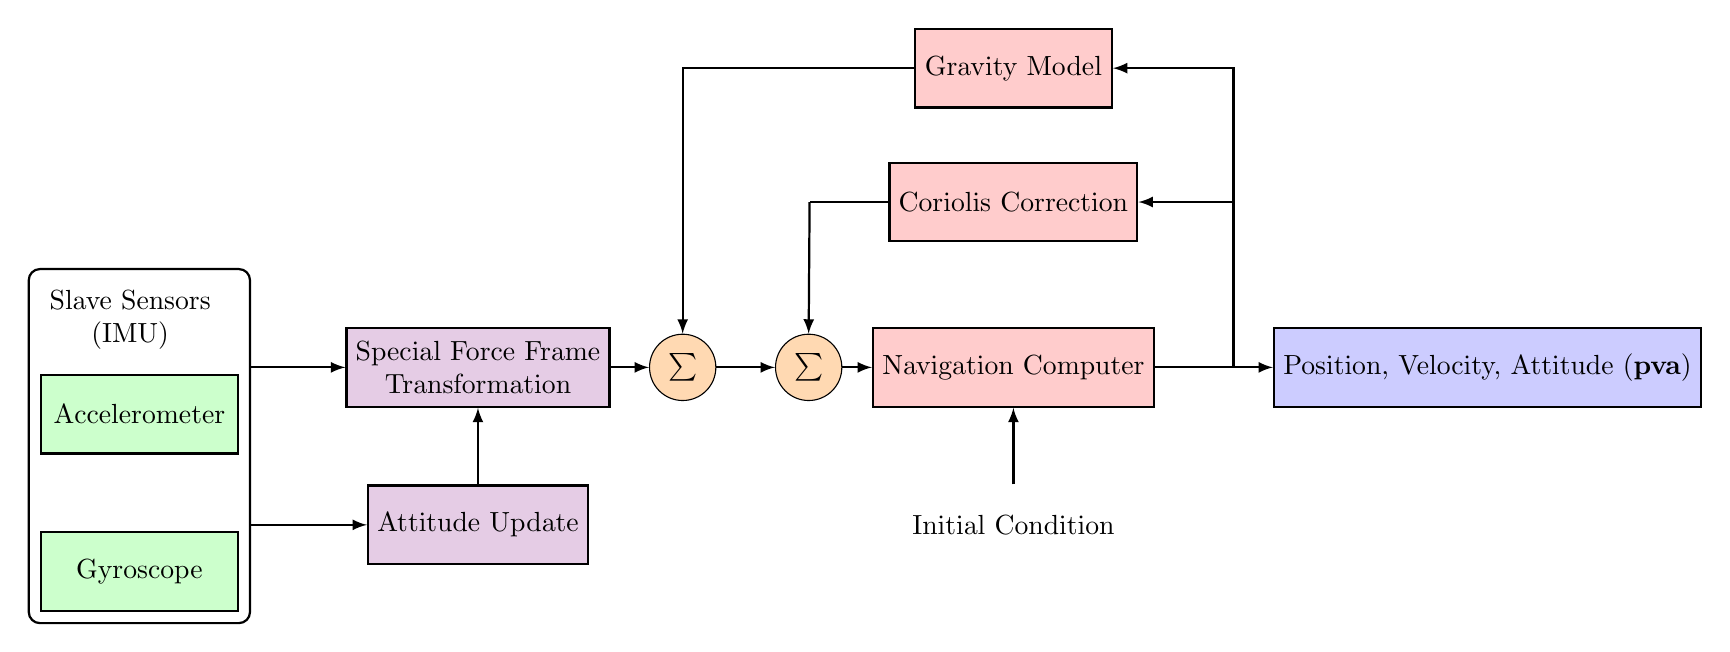
\begin{tikzpicture}

            % Slave
            % Draw the first inner rectangle (below) with start label
            \node[sensor] (Gyroscope) at (3, -3) {Gyroscope};
            
            % Draw the second inner rectangle (above) with stop label
            \node[sensor] (Accelerometer) at (3, -1) {Accelerometer};
        
            % Draw the IMU label above and aligned with Accelerometer
            \node[above=1.2cm of Accelerometer.west, align=center, anchor=west] (IMU) {Slave Sensors\\ (IMU)};
        
            % Draw the outer rectangle tightly around the two inner rectangles
            \node[draw, thick, fit=(Accelerometer) (Gyroscope) (IMU), inner sep=4pt, rounded corners] (IMU_outer) {};
    
            % SINS
            \node[sensor, align=center, fill=violet!20, right of=IMU_outer, xshift=3.3cm, yshift=1cm] 
             (special_force_frame)
              {Special Force Frame\\ Transformation};
              \draw[->, thick] (IMU_outer.east |- special_force_frame.west) -- (special_force_frame.west);

            \node[sensor, align=center, fill=violet!20, right of=IMU_outer, xshift=3.3cm, yshift=-1cm] 
             (attitude_update)
              {Attitude Update};
              \draw[->, thick] (IMU_outer.east |- attitude_update.west) -- (attitude_update.west);
              \draw[->, thick] (attitude_update.north) -- (special_force_frame.south);

              \node[draw, circle,fill=orange!30, right of=special_force_frame, xshift=1.6cm] (sum1)
                  % add sum symbol
                  {$\sum$};
              \draw[->, thick] (special_force_frame.east) -- (sum1.west);
              \node[draw, circle,fill=orange!30, right of=sum1, xshift=.6cm] (sum2)
                  % add sum symbol
                  {$\sum$};
              \draw[->, thick] (sum1.east) -- (sum2.west);
              \node[kf, align=center, fill=red!20, right of=sum2, xshift=1.6cm]
              (nc)
              {Navigation Computer};
              \draw[->, thick] (sum2.east) -- (nc.west);
              % Initial condition node and connection
              \node[sensor, draw=white, fill=violet!0, below of=nc, yshift=-1cm]
              (initial_condition)
              {Initial Condition};
              \draw[->, thick] (initial_condition.north) -- (nc.south);
              \node[kf, align=center, fill=red!20, above of=nc, yshift=1.1cm]
              (coriolis)
              {Coriolis Correction};
              \coordinate (coriolis_in) at ($(nc.east) + (1, 1)$);
              \draw[-, thick] (nc.east) -| (coriolis_in);
              \draw[->, thick] (coriolis_in) |- (coriolis.east);
              \coordinate (coriolis_out) at ($(coriolis.west) + (-1, 0)$);
              \draw[-, thick] (coriolis.west) -| (coriolis_out);
              \draw[->, thick] (coriolis_out) -- (sum2.north);

              \node[kf, align=center, fill=red!20, above of=nc, yshift=2.8cm]
              (gravity)
              {Gravity Model};
              \coordinate (gravity_in) at ($(nc.east) + (1, 1)$);
              \draw[-, thick] (nc.east) -| (gravity_in);
              \draw[->, thick] (gravity_in) |- (gravity.east);
              \coordinate (gravity_out) at ($(sum1.north) + (0, 2)$);
              \draw[-, thick] (gravity.west) -| (gravity_out);
              \draw[->, thick] (gravity_out) -- (sum1.north);
              \node[pva, right =of nc.east, xshift=0.5cm, align=center] (PVA_TA) {Position, Velocity, Attitude (\(\mathbf{pva}\))};
              \draw[->, thick] (nc.east) -- (PVA_TA.west);

        \end{tikzpicture}
  }
  \caption{Structure of the in-motion transfer alignment for the slave vehicle}\label{fig:INS_structure}
  \end{figure}


\subsection{Optimization of Model Structure}
To enhance the performance of the LSTM-based network, an optimization process was conducted using Optuna, an efficient hyperparameter tuning framework. The objective was to determine an optimal architecture by adjusting key hyperparameters, including the number of LSTM layers, the number of units per layer, the depth of the final dense layers, and the learning rate.

\subsubsection{Optimization Strategy}
The model structure was systematically varied, and multiple configurations were evaluated. The key elements of this process included:
\begin{itemize}
    \item The number of LSTM layers was set to 1, 2, or 3 for both input branches.
    \item The number of neurons in each LSTM layer was selected from \{8, 16, 32, 64\}.
    \item The number of dense layers following feature fusion was varied between 1 and 3.
    \item The learning rate was adjusted within the range of $[10^{-4}, 10^{-2}]$.
    \item The best configuration was determined based on the minimum validation loss recorded during training.
\end{itemize}

\subsubsection{Hyperparameter Search Space}
The search space for the optimization is summarized in Table~\ref{tab:hyperparameters}.

\begin{table}[H]
    \centering
    \caption{Hyperparameter Search Space}
    \label{tab:hyperparameters}
    \begin{tabular}{l c}
        \hline
        \textbf{Hyperparameter} & \textbf{Search Range} \\
        \hline
        Number of LSTM layers & \{1, 2, 3\} \\
        Number of neurons per LSTM layer & \{8, 16, 32, 64\} \\
        Number of dense layers & \{1, 2, 3\} \\
        Learning rate & $[10^{-4}, 10^{-2}]$ \\
        \hline
    \end{tabular}
\end{table}

\subsubsection{Implementation Details}
To ensure stable convergence and prevent overfitting, early stopping and batch normalization were applied where necessary. The optimization objective was defined as:
\begin{equation}
    \mathcal{L}_{\text{opt}} = \min \text{val\_loss}
\end{equation}
where $\text{val\_loss}$ represents the lowest validation loss observed during training.



\subsubsection{Results of the Optimization}
Following the optimization process, the best-performing model was identified. The optimal configuration consisted of 2 LSTM layer containing 32 neurons, followed by 2 dense layers with 32 neurons each. A learning rate of approximately 0.01 was found to yield the lowest validation loss. These results indicate that deeper architectures did not always provide superior performance, highlighting the importance of balancing complexity and generalization.

The results of the hyperparameter optimization process are visualized in Fig.~\ref{fig:parallel_plot}, which shows the parallel coordinates plot of different model configurations and their corresponding performance metrics.

\begin{figure}[H]
	\centering
	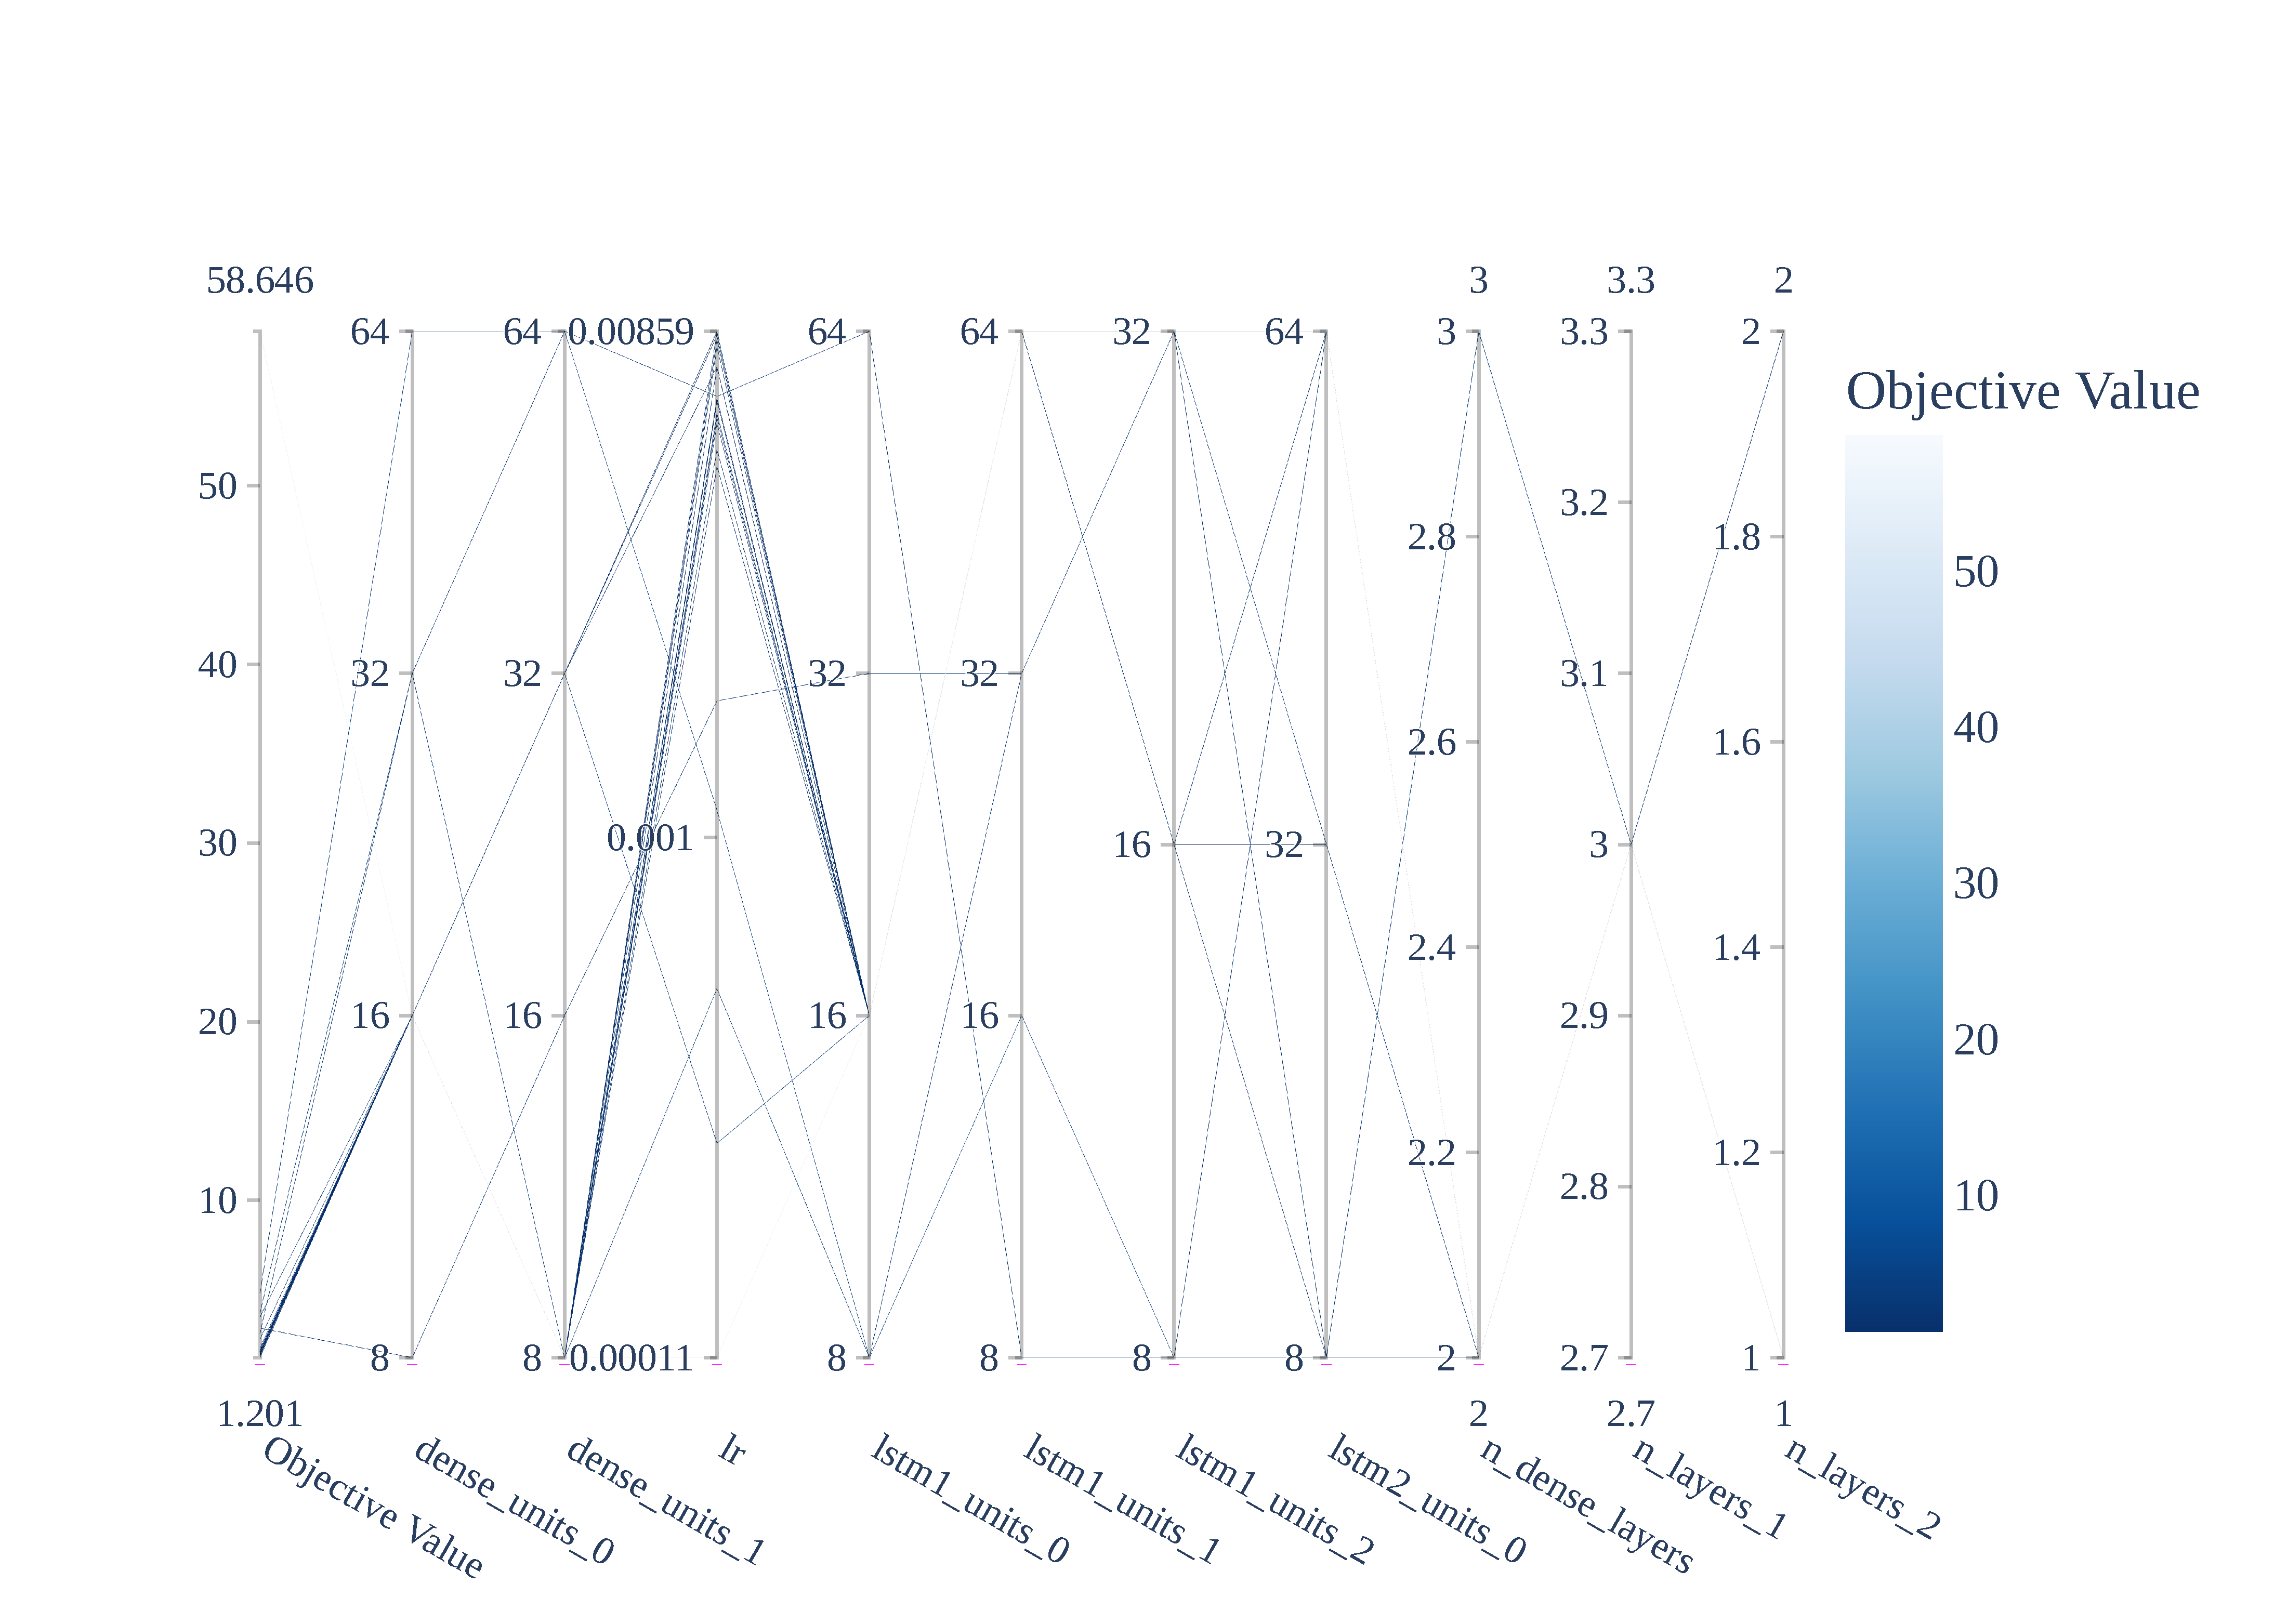
\includegraphics[width=0.7\textwidth]{../Figure/parallel_plot_full.pdf}
	\caption{Parallel coordinates plot showing the relationships between different hyperparameters and model performance. Each line represents a different model configuration, with the color intensity indicating the validation loss (darker colors represent better performance).}
	\label{fig:parallel_plot}
\end{figure}



The optimized model structure demonstrated improved accuracy compared to baseline configurations. The final model was selected based on the best trade-off between validation loss and model complexity, ensuring robust performance on unseen data.

\subsubsection{Model Pruning}
To further optimize the model for deployment, we applied structured pruning techniques to reduce model complexity while maintaining performance. The pruning process involved systematically removing neurons and connections based on their importance to the network's output.

The pruning strategy followed these key steps:
\begin{itemize}
    \item Initial training of the full model to establish baseline performance
    \item Iterative removal of neurons based on L1-norm magnitude
    \item Fine-tuning of the pruned model to recover accuracy
    \item Evaluation against validation data to ensure performance retention
\end{itemize}

The pruning process was guided by a sensitivity threshold \(\tau\), where neurons with L1-norm below \(\tau\) were candidates for removal:
\begin{equation}
    ||w_i||_1 < \tau \implies \text{prune neuron } i
\end{equation}
where \(w_i\) represents the weights connected to neuron \(i\).

Through careful experimentation, we determined that the model could be pruned by approximately 30\% while maintaining 95\% of its original accuracy. The final pruned architecture achieved a more efficient parameter count while preserving the essential predictive capabilities of the network. Table~\ref{tab:pruning_results} summarizes the results of the pruning process.

\begin{table}[H]
    \centering
    \caption{Model Pruning Results}
    \label{tab:pruning_results}
    \begin{tabular}{l c c}
        \hline
        \textbf{Metric} & \textbf{Original Model} & \textbf{Pruned Model} \\
        \hline
        Parameter Count & 46,825 & 32,778 \\
        Inference Time (ms) & 12.3 & 8.9 \\
        Validation Loss & 0.2298 & 0.2412 \\
        Model Size (KB) & 182.91 & 128.04 \\
        \hline
    \end{tabular}
\end{table}

The pruned model demonstrated comparable performance to the original while offering improved computational efficiency, making it more suitable for deployment in resource-constrained environments.



\subsection{GPS Outages}
\noindent When the GPS signal is available, the data of the master navigation unit including the estimated position, \(\hat{\mathbf{p}}_{(t_1)}\), velocity, \(\hat{\mathbf{v}}_{(t_1)}\), and attitude, \(\hat{\mathbf{a}}_{(t_1)}\), at sample time \(t_1 < t\) and the measurement of the master's IMU for all sample time (0 to t), are stored in the database as the input.
% , according to Fig~\ref{fig:NN_structure}.
This information is trained using a Neural Network (NN) approach to produce a model for the prediction phase based on the finding the least square solution of the difference between the estimated outputs, obtained by master navigation unit (equations~\eqref{eq:kalman_1}-\eqref{eq:kalman_2}~and~\eqref{eq:kalman_3}-\eqref{eq:kalman_6}) at sample time \(t\), \(\hat{\mathbf{\mathrm{y}}}_{(t)} = \{ \hat{\mathbf{v}}_{\mathbf{M}}, \hat{\mathbf{p}}_{\mathbf{M}}, \hat{\mathbf{a}}_{\mathbf{M}} \}\), with the predicted data, \(\mathbf{{y}}_{(t)}\), obtained by proposed NN as follows:
\begin{equation}
	\mathrm{loss}_{(t)} = || \hat{\mathbf{{y}}}_{(t)} - \mathbf{{y}}_{(t)} ||^2.
\end{equation}

The structure of the proposed NN is shown in Fig~\ref{fig:NN_structure}.
This structure is utilized in the master navigation unit to predict the position, velocity, and attitude in the absence of the GPS signal, as shown in Fig~\ref{fig:master_prediction}.
In the following, subsystems of the proposed NN are detailed.
%%%%%%%%%% here NN %%%%%%%%
\begin{figure}[H]
	\centering	
	

\resizebox{1\textwidth}{!}{
	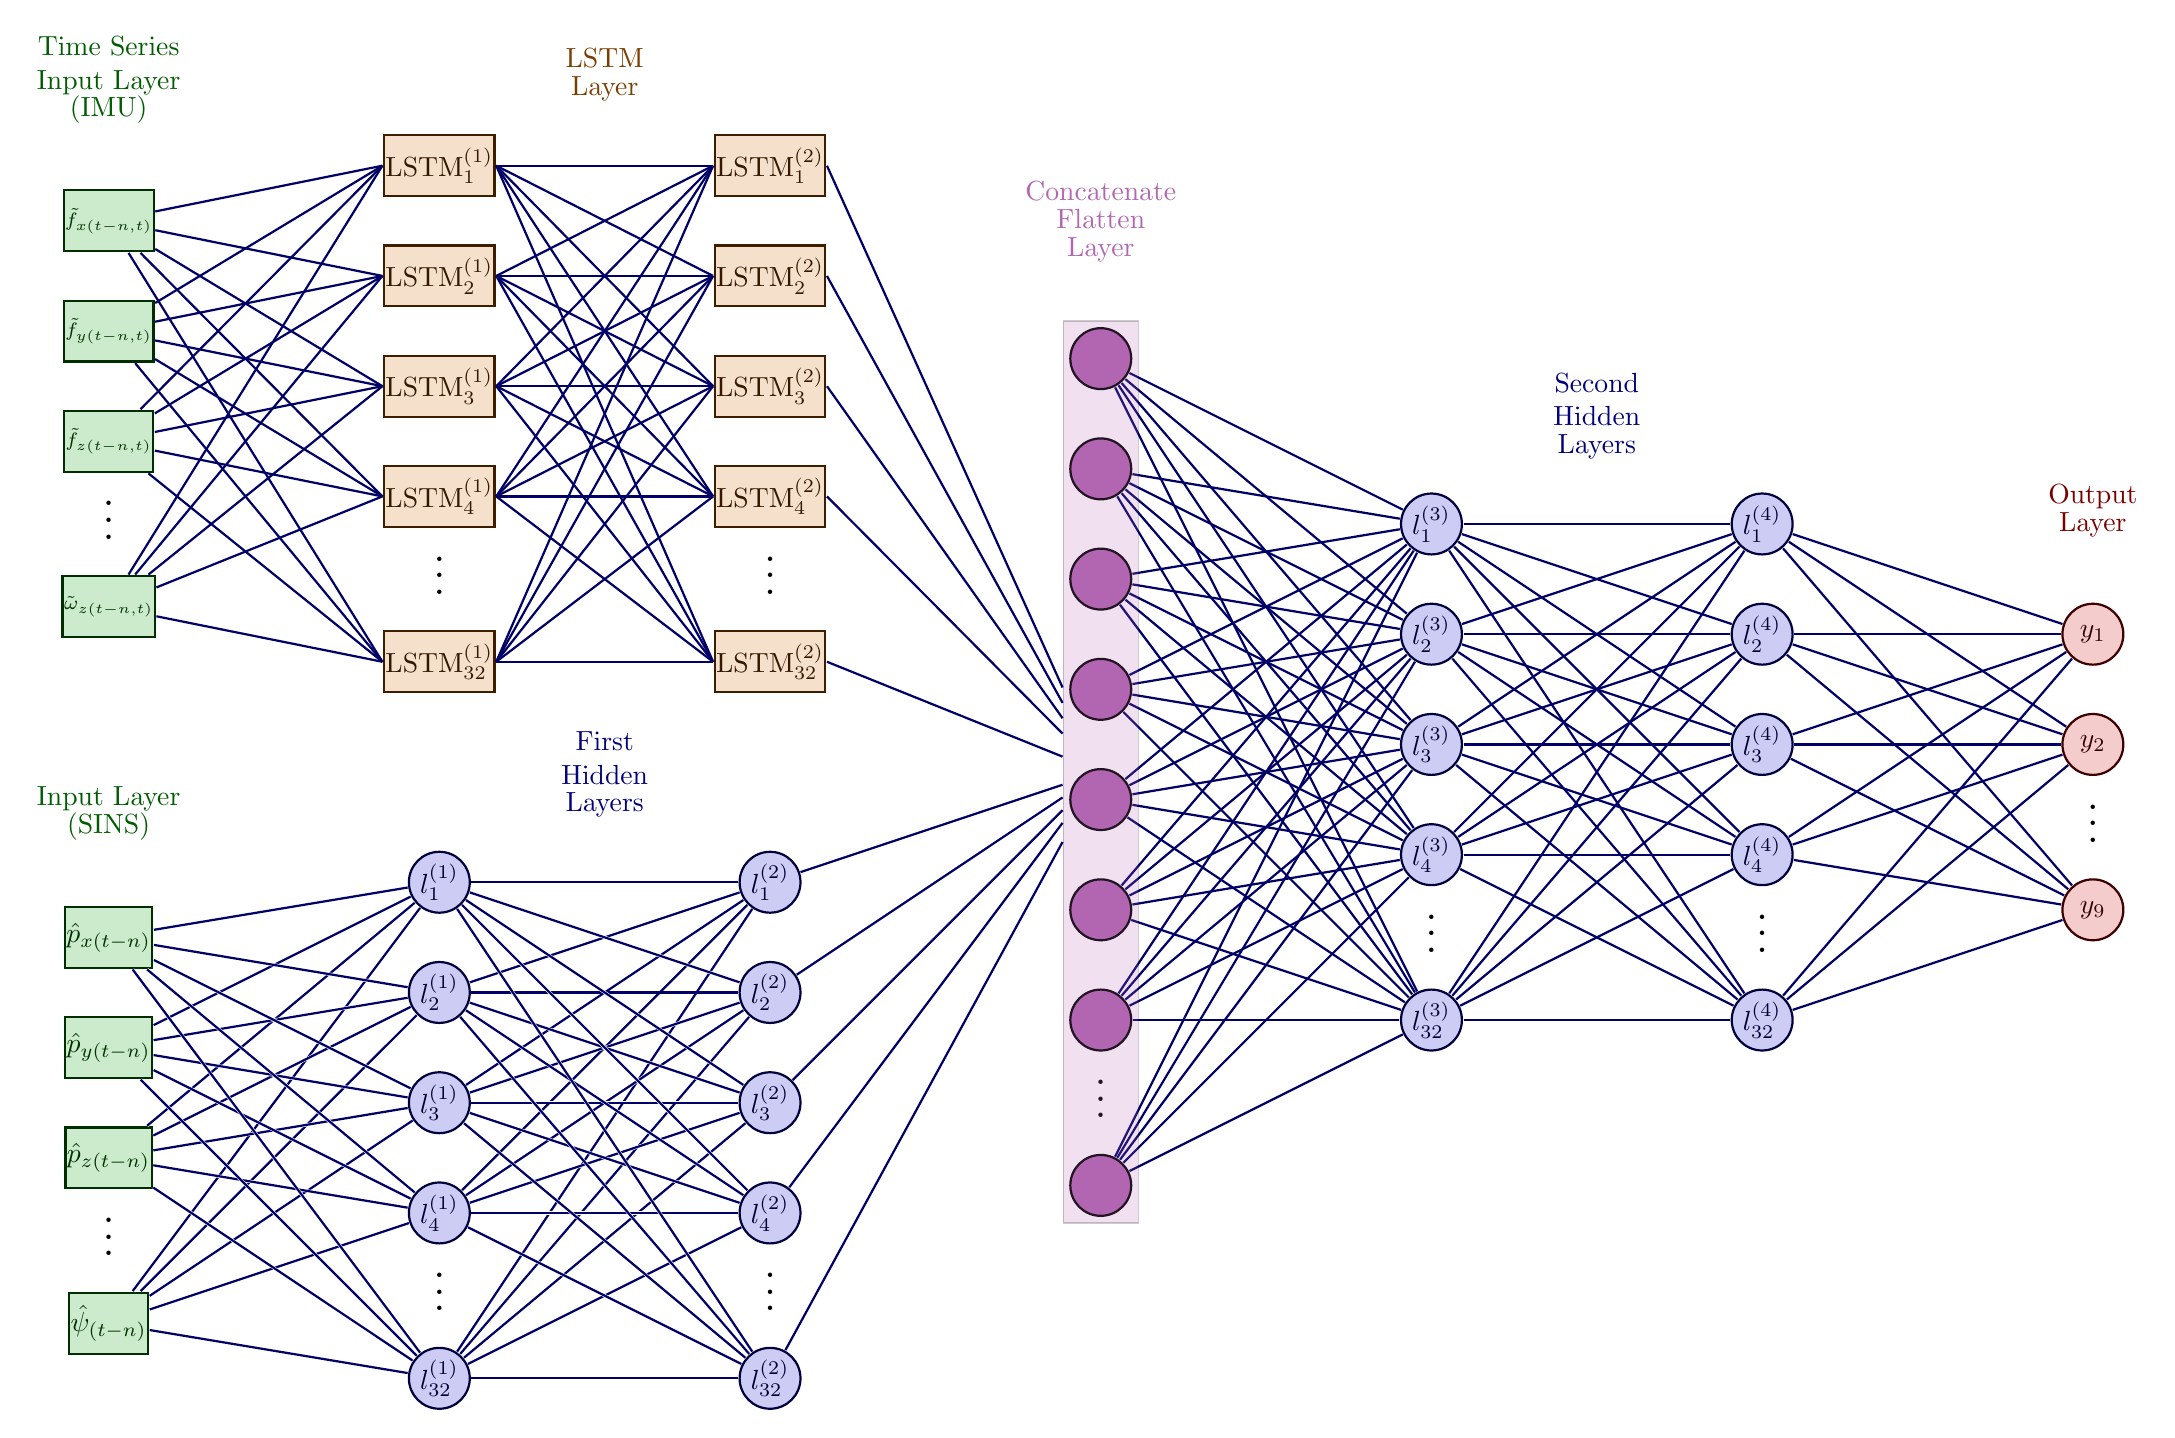
\begin{tikzpicture}[x=4.2cm,y=1.4cm]
		% \message{^^JNeural network, shifted}
		\readlist\Nnod{4,5,5} % array of number of nodes per layer
		\readlist\Nstr{9,32,32} % array of string number of nodes per layer
		\readlist\ins{\hat{p}_{x(t-n)},
		\hat{p}_{y(t-n)},
		\hat{p}_{z(t-n)},
		\hat{\psi}_{(t-n)}}
		\readlist\Cstr{\strut x,l^{(\prev)},l^{(\prev)}} % array of coefficient symbol per layer
		\def\yshift{0.5} % shift last node for dots

		\message{^^J  Layer}
		\foreachitem \N \in \Nnod{ % loop over layers
		  \def\lay{\Ncnt} % alias of index of current layer
		  \pgfmathsetmacro\prev{int(\Ncnt-1)} % number of previous layer
		  \message{\lay,}
		  \foreach \i [evaluate={\c=int(\i==\N); \y=\N/2-\i-\c*\yshift;
					   \index=(\i<\N?int(\i):"\Nstr[\lay]");
					   \x=\lay; \n=\nstyle;}] in {1,...,\N}{ % loop over nodes
			% NODES
			\ifnum\lay=1
			  \node[node in,green!20!black,draw=mygreen!30!black,fill=mygreen!20, rectangle
			  ] (N\lay-\i) at (\x,\y) {$\ins[\i]$};
			\else
				\node[node hidden] (N\lay-\i) at (\x,\y) {$\Cstr[\lay]_{\index}$};
			\fi

			% CONNECTIONS
			\ifnum\lay>1 % connect to previous layer
			  \foreach \j in {1,...,\Nnod[\prev]}{ % loop over nodes in previous layer
				\draw[connect,white,line width=1.2] (N\prev-\j) -- (N\lay-\i);
				\draw[connect] (N\prev-\j) -- (N\lay-\i);
				%\draw[connect] (N\prev-\j.0) -- (N\lay-\i.180); % connect to left
			  }
			\fi % else: nothing to connect first layer

		  }
		  \path (N\lay-\N) --++ (0,1+\yshift) node[midway,scale=1.5] {$\vdots$};
		}

		%%%%%%%%%%%%%%%%%%%
		\def\lowerlstm{-6.5}
		%%%%%%%%%%%%%%%%%%%


		\def\Nnodlstm{4}
		\def\Nstrlstm{6}
		\readlist\imu{
		\tilde{f}_{x(t-n,t)},
		\tilde{f}_{y(t-n,t)},
		\tilde{f}_{z(t-n,t)},
		\tilde{\omega}_{z(t-n,t)}}
		% add new input layer
		\foreach \i [evaluate={\c=int(\i==\Nnodlstm); \y=\Nnodlstm/2-\i-\c*\yshift-\lowerlstm;
					 \index=(\i<\Nnodlstm?int(\i):"\Nstrlstm");
					 \x=1; \n=\nstyle;}] in {1,...,\Nnodlstm}{
		  \node[node in,green!20!black,draw=mygreen!30!black,fill=mygreen!20, rectangle
		  ] (N0lstm-\i) at (\x,\y) {\scriptsize ${\imu[\i]}$};
		}
		\path (N0lstm-\Nnodlstm) --++ (0,1+\yshift) node[midway,scale=1.5] {$\vdots$};

		% LSTM layer
		\def\Nnodlen{5}
		\def\Nstrlen{32}
		\foreach \i [evaluate={\c=int(\i==\Nnodlen); \y=\Nnodlen/2-\i-\c*\yshift-\lowerlstm;
					 \index=(\i<\Nnodlen?int(\i):"\Nstrlen");
					 \x=2; \n=\nstyle;}] in {1,...,\Nnodlen}{
		  \node[node LSTM] (N1lstm-\i) at (\x,\y) {$\text{LSTM}^{(1)}_{\index}$};
		}
		\path (N1lstm-\Nnodlen) --++ (0,1+\yshift) node[midway,scale=1.5] {$\vdots$};

		% connections
		\foreach \i in {1,...,\Nnodlstm}{
		  \foreach \j in {1,...,\Nnodlen}{
			% connect to left side
			\draw[connect] (N0lstm-\i) -- (N1lstm-\j.180);
		  }
		}

		% LSTM layer 2
		\def\Nnodlen{5}
		\def\Nstrlen{32}
		\foreach \i [evaluate={\c=int(\i==\Nnodlen); \y=\Nnodlen/2-\i-\c*\yshift-\lowerlstm;
					 \index=(\i<\Nnodlen?int(\i):"\Nstrlen");
					 \x=3; \n=\nstyle;}] in {1,...,\Nnodlen}{
		  \node[node LSTM] (N2lstm-\i) at (\x,\y) {$\text{LSTM}^{(2)}_{\index}$};
		}
		\path (N2lstm-\Nnodlen) --++ (0,1+\yshift) node[midway,scale=1.5] {$\vdots$};

		% connections
		\foreach \i in {1,...,\Nnodlen}{
		  \foreach \j in {1,...,\Nnodlen}{
			% connect to left side
			\draw[connect] (N1lstm-\i.0) -- (N2lstm-\j.180);
		  }
		}

		% concatenate layer
		\def\Nnodlenc{8}
		\def\Nstrlen{32}
		\foreach \i [evaluate={\c=int(\i==\Nnodlenc); \y=\Nnodlenc/2-\i-\c*\yshift-\lowerlstm/2;
					 \index=(\i<\Nnodlenc?int(\i):"\Nstrlen");
					 \x=4; \n=\nstyle;}] in {1,...,\Nnodlenc}{
		  \node[node, fill=myviolet, draw=black]
		   (Nc-\i) at (\x,\y) {};
		}
		\path (Nc-\Nnodlenc) --++ (0,1+\yshift) node[midway,scale=1.5] {$\vdots$};


		% hidden layer
		\def\Nnodlen{5}
		\def\Nstrlen{32}
		\foreach \i [evaluate={\c=int(\i==\Nnodlen); \y=\Nnodlen/2-\i-\c*\yshift-\lowerlstm/2;
					 \index=(\i<\Nnodlen?int(\i):"\Nstrlen");
					 \x=5; \n=\nstyle;}] in {1,...,\Nnodlen}{
		  \node[node hidden] (N4-\i) at (\x,\y) {${l}^{(3)}_{\index}$};
		}
		\path (N4-\Nnodlen) --++ (0,1+\yshift) node[midway,scale=1.5] {$\vdots$};

		% connections
		\foreach \i in {1,...,\Nnodlenc}{
		  \foreach \j in {1,...,\Nnodlen}{
			% connect to left side
			\draw[connect] (Nc-\i) -- (N4-\j);
		  }
		}

		% add box for concatenate layer
		\node[draw=black,fit=(Nc-1)(Nc-\Nnodlenc),inner sep=2pt,fill=myviolet,opacity=0.2] (boxc) {};

		% connections
		\foreach \i in {1,...,\Nnodlen}{
			% connect to left north side
			\draw[connect] (N2lstm-\i.0) -- (boxc);
		}
		\foreach \i in {1,...,\Nnod[3]}{
			% connect to left south side
			\draw[connect] (N3-\i) -- (boxc);
		}

		% hidden layer
		\def\Nnodlen{5}
		\def\Nstrlen{32}
		\foreach \i [evaluate={\c=int(\i==\Nnodlen); \y=\Nnodlen/2-\i-\c*\yshift-\lowerlstm/2;
					 \index=(\i<\Nnodlen?int(\i):"\Nstrlen");
					 \x=6; \n=\nstyle;}] in {1,...,\Nnodlen}{
		  \node[node hidden] (N5-\i) at (\x,\y) {${l}^{(4)}_{\index}$};
		}
		\path (N5-\Nnodlen) --++ (0,1+\yshift) node[midway,scale=1.5] {$\vdots$};

		% connections
		\foreach \i in {1,...,\Nnodlen}{
		  \foreach \j in {1,...,\Nnodlen}{
			% connect to left side
			\draw[connect] (N4-\i) -- (N5-\j);
		  }
		}

		% output layer
		\def\Nnodlenc{3}
		\def\Nstrlen{9}
		\foreach \i [evaluate={\c=int(\i==\Nnodlenc); \y=\Nnodlenc/2-\i-\c*\yshift-\lowerlstm/2;
					 \index=(\i<\Nnodlenc?int(\i):"\Nstrlen");
					 \x=7; \n=\nstyle;}] in {1,...,\Nnodlenc}{
		  \node[node out] (N6-\i) at (\x,\y) {${y}_{\index}$};
		}
		\path (N6-\Nnodlenc) --++ (0,1+\yshift) node[midway,scale=1.5] {$\vdots$};

		% connections
		\foreach \i in {1,...,\Nnodlen}{
		  \foreach \j in {1,...,\Nnodlenc}{
			% connect to left side
			\draw[connect] (N5-\i) -- (N6-\j);
		  }
		}

		% % LABELS
		\node[above=2em,align=center,mygreen!60!black] at (N1-1.90) {Input Layer\\[-0.2em](SINS)};
		% second input layer
		\node[above=2em,align=center,mygreen!60!black] at (N0lstm-1.90) {Time Series\\Input Layer\\[-0.2em](IMU)};
		% layer between LSTM
		\path (N1lstm-1) coordinate (coord0);
		\path (N2lstm-1) coordinate (coord1);
		\node[above=2em,align=center,myorange!60!black] at ($(coord0)!0.5!(coord1)$) {LSTM\\[-0.2em]Layer};
		% hidden layer
		\path (N2-1) coordinate (coord0);
		\path (N3-1) coordinate (coord1);
		\node[above=2em,align=center,myblue!60!black] at ($(coord0)!0.5!(coord1)$) {First\\ Hidden\\[-0.2em]Layers};
		% concatenate layer
		\node[above=2em,align=center,myviolet] at (Nc-1.90) {Concatenate\\[-0.2em]Flatten\\[-0.2em]Layer};
		% last hidden layer
		\path (N5-1) coordinate (coord0);
		\path (N4-1) coordinate (coord1);

		\node[above=2em,align=center,myblue!60!black] at ($(coord0)!0.5!(coord1)$) {Second\\ Hidden\\[-0.2em]Layers};
		\node[above=2em,align=center,myred!60!black] at (N6-1.90) {Output\\[-0.2em]Layer};
	  \end{tikzpicture}
	  }
		  % Caption for the structure of the Proposed Neural Network.
		  \caption{Structure of the Proposed Modular Neural Network.}\label{fig:NN_structure}
\end{figure}



% \begin{figure}[H]
% 	\centering
% 	\includegraphics[width=0.5\textwidth]{../Diagrams/full_strruct.pdf}
% 	\caption{Structure of Master Navigation Unit in the Prediction Phase}
% 	\label{fig:master_prediction}
% \end{figure}

\begin{figure}[H]
	\centering
	\resizebox{.5\textwidth}{!}
    {
        \begin{tikzpicture}


        \node[sensor] (IMU) at (3, 3) {IMU};
        \node[sensor, align=center, fill=violet!20, right of=IMU, xshift=3.3cm]
            (SINS)
            {SINS of the Master Vehicle};

        % connect IMU and SINS
        \draw[->, thick] (IMU) -- (SINS);

        % AI node with figure in it
        \node[draw, thick, fill=blue!0, minimum width=2.5cm, minimum height=1cm, right of=SINS, xshift=3.3cm]
            (AI)
            {
\includegraphics[width=1.5cm]{../Figure/AI.pdf}};

        % connect SINS and AI
        \draw[->, thick] (SINS) -- (AI);

        \coordinate[below=.85cm of IMU] (bottom);
        \coordinate[above=.85cm of SINS] (up);
		\coordinate[right=1cm of AI] (right);
		\coordinate[right=2cm of AI] (right1);

        % connect IMU to AI
        \draw[->, thick] (IMU) |- (bottom) -| (AI);

        % connect AI to SINS
        \draw[->, thick] (AI.0) -- (right) |- (up) -| (SINS) node[midway, above] {PVA };

		\draw[->, thick] (AI.0) -- (right1) node[at end, above] {PVA};




        \end{tikzpicture}
    }
	\caption{Structure of Master Navigation Unit in the Prediction Phase}\label{fig:master_prediction}
\end{figure}

\subsection{Multilayer Neural Network}
\noindent The proposed NN consists of three main layers, including the input layer, LSTM layer, and output layer, as shown in Fig~\ref{fig:NN_structure}.
The input layer is fed by the estimated states of the master's SINS, including the position, velocity, and attitude, and the IMU outputs.
The LSTM layer is utilized to capture the time-series data of the IMU outputs.
The output layer is used to predict the position, velocity, and attitude of the master's SINS in the absence of the GPS signal.
The proposed NN is trained using the data obtained from the master navigation unit, including the estimated states of the master's SINS and the IMU outputs, to predict the position, velocity, and attitude of the master's SINS in the absence of the GPS signal.

\subsubsection{LSTM Layer Architecture}
\noindent Here, a model is generated based on the multilayer Long-Short Term Memory (LSTM), according to Fig~\ref{fig:NN_structure}, using the sequential data including IMU outputs and estimated states obtained from KF\@.
LSTM~\cite{LSTM} is a class of the Recurrent Neural Network (RNN), that retains selectively and utilizes relevant information, while discarding noisy data. This architecture of the LSTM cell structure, consists of the memory cell and gating mechanisms, is illustrated in Fig~\ref{fig:LSTM_in_layer}.

% \begin{figure}[H]
% 	\centering
% 	\includegraphics[width=0.5\textwidth]{../Diagrams/LSTM_struct.pdf}
% 	\caption{Structure of Multilayer LSTM applied in proposed method}
% 	\label{fig:LSTM_structure}
% \end{figure}


\begin{figure}[H]
	\centering
	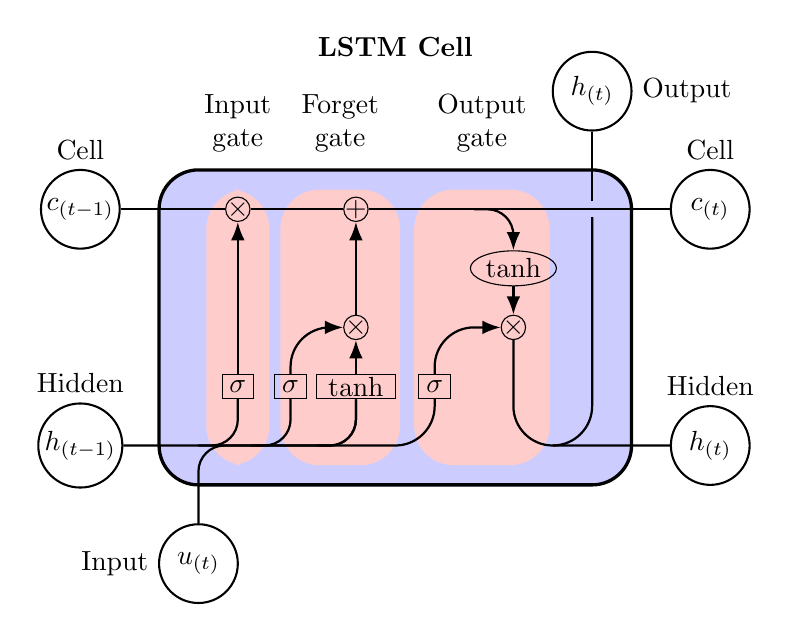
\begin{tikzpicture}[
		>=Latex,
		cell/.style={
			rectangle,
			rounded corners=5mm,
			draw,
			very thick,
			minimum height=4cm,
			minimum width=6cm,
		},
		operator/.style={
			circle,
			draw,
			inner sep=-0.5pt,
			minimum height=.2cm,
		},
		function/.style={
			ellipse,
			draw,
			inner sep=1pt,
		},
		ct/.style={
			circle,
			draw,
			line width=.75pt,
			minimum width=1cm,
			inner sep=1pt,
		},
		gt/.style={
			rectangle,
			draw,
			minimum width=4mm,
			minimum height=3mm,
			inner sep=1pt,
		},
		ArrowC1/.style={
			rounded corners=.33cm,
			thick,
		},
		ArrowC2/.style={
			rounded corners=.5cm,
			thick,
		},
		]

		% Draw the cell:
		\node (lstm_cell) [cell, fill=blue!20] at (0,0) {};
		\node (Cell_laybel) [above=1.3cm of lstm_cell] {\textbf{LSTM Cell}};

		% Draw inputs named ibox#
		\node (r1) [cell, draw=none, fill=red!20, minimum width=0.8cm,minimum height=3.5cm] at (-2, 0) {};
		\node (r2) [cell, draw=none, fill=red!20, minimum width=1.52cm,minimum height=3.5cm] at (-0.7, 0) {};
		\node (r3) [cell, draw=none, fill=red!20, minimum width=1.72cm,minimum height=3.5cm] at (1.1, 0) {};
		2
		\node (r1Label) [above=0.33cm of r1, align=center] {Input\\ gate};
		\node (r2Label) [above=0.33cm of r2, align=center] {Forget\\ gate};
		\node (r3Label) [above=0.33cm of r3, align=center] {Output\\ gate};


		\node [gt] (ibox1) at (-2,-0.75) {$\sigma$};
		\node [gt] (ibox2) at (-1.33,-0.75) {$\sigma$};
		\node [gt, minimum width=1cm] (ibox3) at (-0.5,-0.75) {$\tanh$};
		\node [gt] (ibox4) at (0.5,-0.75) {$\sigma$};

		% Draw operators named mux#, add#, and func#
		\node [operator] (mux1) at (-2,1.5) {$\times$};
		\node [operator] (add1) at (-0.5,1.5) {+};
		\node [operator] (mux2) at (-0.5,0) {$\times$};
		\node [operator] (mux3) at (1.5,0) {$\times$};
		\node [function] (func1) at (1.5,0.75) {$\tanh$};
		\node[ct, label={Cell}] (c) at (-4,1.5) {\({c}_{(t-1)}\)};
		\node[ct, label={Hidden}] (h) at (-4,-1.5) {\({h}_{(t-1)}\)};
		\node[ct, label={left:Input}] (x) at (-2.5,-3) {\({u}_{(t)}\)};

		% Draw external outputs named c2, h2, x2
		\node[ct, label={Cell}] (c2) at (4,1.5) {\({c}_{(t)}\)};
		\node[ct, label={Hidden}] (h2) at (4,-1.5) {\({h}_{(t)}\)};
		\node[ct, label={right:Output}] (x2) at (2.5,3) {\({h}_{(t)}\)};

		% Start connecting everything.
		% Use intersections and displacements for clarity.

		% Drawing arrows
		\draw [ArrowC1] (c) -- (mux1) -- (add1) -- (c2);

		% Inputs
		\draw [ArrowC2] (h) -| (ibox4);
		\draw [ArrowC1] (h -| ibox1)++(-0.5,0) -| (ibox1);
		\draw [ArrowC1] (h -| ibox2)++(-0.5,0) -| (ibox2);
		\draw [ArrowC1] (h -| ibox3)++(-0.5,0) -| (ibox3);
		\draw [ArrowC1] (x) -- (x |- h)-| (ibox3);

		% Internal
		\draw [->, ArrowC2] (ibox1) -- (mux1);
		\draw [->, ArrowC2] (ibox2) |- (mux2);
		\draw [->, ArrowC2] (ibox3) -- (mux2);
		\draw [->, ArrowC2] (ibox4) |- (mux3);
		\draw [->, ArrowC2] (mux2) -- (add1);
		\draw [->, ArrowC1] (add1 -| func1)++(-0.5,0) -| (func1);
		\draw [->, ArrowC2] (func1) -- (mux3);

		% Outputs
		\draw [-, ArrowC2] (mux3) |- (h2);
		\draw (c2 -| x2) ++(0,-0.1) coordinate (i1);
		\draw [-, ArrowC2] (h2 -| x2)++(-0.5,0) -| (i1);
		\draw [-, ArrowC2] (i1)++(0,0.2) -- (x2);

	\end{tikzpicture}
	\caption{LSTM cell structure}\label{fig:LSTM_in_layer}
\end{figure}

In this structure, the relationship  between, the output, \(\mathbf{y}_{{\text{LSTM}}_{{(t)}}}\), and input, \(\mathbf{u}_{(t)}\) is computed based on the sigmoid function, \(\sigma\), as
\begin{equation}
	\mathbf{y}_{(t)} = \sigma(\mathbf{W}_{\text{LSTM}} \cdot [\mathbf{h}_{(t-1)}, \mathbf{u}_{(t)}] + \mathbf{b}_{\text{LSTM}}),
\end{equation}
where \(\mathbf{W}_{\text{LSTM}}\) and \(\mathbf{b}_{\text{LSTM}}\) are, respectively, the weight matrix and bias vector.
Moreover, \(\mathbf{h}_{(t-1)}\) denotes the previous hidden state, containing the output information at sample time t, is updated as
\begin{equation}
	\mathbf{h}_{(t)} = \mathbf{o}_{(t)} \odot \tanh(\mathbf{c}_{(t)}),
\end{equation}
where notation \(\odot\) is element wise product and \(\mathbf{c}_{(t)}\) is memory cell at sample time t, that retains the relevant information and is propagated as follows:
\begin{equation}
	\mathbf{c}_{(t)} = \mathbf{f}_{\text{g}(t)} \odot \mathbf{c}_{(t-1)} + \mathbf{i}_{(t)} \odot \tanh(\mathbf{W}_c \cdot [\mathbf{h}_{(t-1)}, \mathbf{u}_{(t)}] + \mathbf{b}_c).
\end{equation}
% here \(\mathbf{\tilde{c}_{(t)}}\) denotes the cell state, that is between -1 and 1, is computed as
% \begin{equation}
% 	\mathbf{\tilde{c}}_{(t)} = \tanh(\mathbf{W}_c \cdot [\mathbf{h}_{(t-1)}, \mathbf{X}_{(t)}] + \mathbf{b}_c)
% \end{equation}
Moreover, \(\mathbf{W}_c\) and \(\mathbf{b}_c\) are, respectively, the weight matrix and bias vector. Also, \(\mathbf{i_{(t)}}\) and \(\mathbf{f_{\text{g}(t)}}\) denote the input and forget gates to regulate the information flow and are computed based on the sigmoid function, \(\sigma\), as follows:
\begin{equation}
	\mathbf{i}_{(t)} = \sigma(\mathbf{W}_i \cdot [\mathbf{h}_{(t-1)}, \mathbf{u}_{(t)}] + \mathbf{b}_i),
\end{equation}
\begin{equation}
	\mathbf{f}_{\text{g}(t)} = \sigma(\mathbf{W}_{f_{\text{g}}} \cdot [\mathbf{h}_{(t-1)}, \mathbf{u}_{(t)}] + \mathbf{b}_{f_{\text{g}}}),
\end{equation}
where \(\mathbf{W}_j\) and \(\mathbf{b}_j\) for (\(j=i, f_{\text{g}} \)) are weight matrix and bias vectors, respectively.
% complete`'
Moreover, \( \mathbf{h}_{(t)} \) and \( \mathbf{c}_{(t)} \) are two outputs of
an LSTM unit, which are called the hidden state and cell state, respectively.
\begin{align}
\mathbf{h}_{(t)} &= \mathbf{o}_{(t)} \odot \tanh(\mathbf{c}_{(t)}), \\
\mathbf{c}_{(t)} &= \mathbf{f}_{\text{g}(t)} \odot \mathbf{c}_{(t-1)} + \mathbf{i}_{(t)} \odot \tilde{\mathbf{c}}_{(t)},
\end{align}
where \( \mathbf{i}_{(t)} \), \( \mathbf{o}_{(t)} \), \( \mathbf{f}_{\text{g}(t)} \), and \( \tilde{\mathbf{c}}_{(t)} \) represent the input gate, output gate, forget gate, and cell candidate state, defined as follows:
\begin{align}
\mathbf{i}_{(t)} &= \sigma(\mathbf{W}_i \cdot [\mathbf{h}_{(t-1)}, \mathbf{x}_{(t)}] + \mathbf{b}_i). \\
% \mathbf{o}_{(t)} &= \sigma(\mathbf{W}_o \cdot [\mathbf{h}_{(t-1)}, \mathbf{x}_{(t)}] + \mathbf{b}_o) \\
% \mathbf{f}_{\text{g}(t)} &= \sigma(\mathbf{W}_f \cdot [\mathbf{h}_{(t-1)}, \mathbf{x}_{(t)}] + \mathbf{b}_{f_\text{g}}) \\
% \tilde{\mathbf{c}}_{(t)} &= \tanh(\mathbf{W}_c \cdot [\mathbf{h}_{(t-1)}, \mathbf{x}_{(t)}] + \mathbf{b}_c)
\end{align}
At the final time step, the hidden state \( \mathbf{h}_{(t_{\text{final}})} \) is passed to the next layer.



% \begin{equation}
% \text{{Concatenate}}(y_1, y_2) = \text{{concatenated\_output}}
% \end{equation}
% where $\text{{concatenated\_output}}$ is the resulting tensor after concatenation. This concatenated tensor can then be passed to subsequent layers for further processing.






% The Flatten function in TensorFlow is represented by the equation:
% \begin{equation}
% \text{{Flatten}}(x) = x_{\text{{flattened}}}
% \end{equation}
% where $x$ is the input tensor with dimensions $(\text{{height}}, \text{{width}}, \text{{channels}})$, and $x_{\text{{flattened}}}$ is the flattened output tensor, a one-dimensional array.

\subsubsection{Dense Layer Functionality}
\noindent According to Fig~\ref{fig:NN_structure}, two dense layers neural networks, that are fully connected, are utilized
with two sub-layers.
First dense layers process the SINS outputs of the master vehicle \(
(\mathbf{p_M}, \mathbf{v_M}, \mathbf{a_M})
\)
to produce the following outputs:
\begin{equation}
\mathbf{u}_{\text{dense}}  = \sigma(\mathbf{W}_{\text{dense}_2} \cdot \sigma(\mathbf{W}_{\text{dense}_1} \cdot
	[\hat{\mathbf{p}}, \hat{\mathbf{v}}, \hat{\mathbf{a}}]
	 + \mathbf{b}_{\text{dense}_1}) + \mathbf{b}_{\text{dense}_2}).
\end{equation}
The second dense layers use flatten concatenated outputs
(\(\mathbf{u}_{\text{flatten}} =
\left[
	\mathbf{u}_{\text{LSTM}},
	\mathbf{u}_{\text{dense}}
\right]
\)) which convert a multidimensional tensor into a one-dimensional tensor, to generate the desired outputs as follows:
\begin{equation}
\mathbf{y} = \sigma(\mathbf{w}_{\text{dense}_4} \cdot \sigma(\mathbf{w}_{\text{dense}_3} \cdot \mathbf{u}_{\text{flatten}}
	 + \mathbf{b}_{\text{dense}_3}) + \mathbf{b}_{\text{dense}_4}).
\end{equation}

% \noindent Dense layer neural network is a fully connected layer, where each neuron is connected to all the neurons in the previous layer.
% The dense layer is utilized to process the SINS outputs (\(\mathbf{pva}\)) and the outputs of the LSTM
% (\(\mathbf{u}_{\text{LSTM}}\))
% and the first dense hidden layer
% (\(\mathbf{u}_{\text{dense}}\)), which are then concatenated and flattened
% (\(\mathbf{u}_{\text{flatten}} =
% \left[
% 	\mathbf{u}_{\text{LSTM}},
% 	\mathbf{u}_{\text{dense}}
% \right]
% \)), respectively.

% The output of the first and second dense layer is computed as follows:
% \begin{align}
% 	\mathbf{u}_{\text{dense}} & = \sigma(\mathbf{W}_{\text{dense}_2} \cdot \sigma(\mathbf{W}_{\text{dense}_1} \cdot
% 	[\hat{\mathbf{p}}, \hat{\mathbf{v}}, \hat{\mathbf{a}}]
% 	& \hspace{-3.3cm}+ \mathbf{b}_{\text{dense}_1}) + \mathbf{b}_{\text{dense}_2}) \\
% 	\mathbf{y} &= \sigma(\mathbf{w}_{\text{dense}_4} \cdot \sigma(\mathbf{w}_{\text{dense}_3} \cdot \mathbf{u}_{\text{flatten}}
% 	& \hspace{-3.3cm} + \mathbf{b}_{\text{dense}_3}) + \mathbf{b}_{\text{dense}_4})
% \end{align}

% \subsubsection{Concatenate and Flatten}
% % Let $NN_1$ and $NN_2$ be two neural networks. The output tensors of $NN_1$ and $NN_2$ are denoted as $y_1$ and $y_2$, respectively. To concatenate these neural networks, we use the Concatenate function in TensorFlow, represented as:
% \noindent According to Fig~\ref{fig:NN_structure}, the outputs of two neural network layers (the LSTM layer and the first dense hidden layer) are concatenated and flattened which is called \(\boldsymbol{u}_{\mathrm{flatten}}\) to be processed by the final hidden layer.


\section{Structure of the Motion Alignment}
\noindent After the accurate navigation of the master vehicle, the process of the transfer alignment approach, according to Fig~\ref{fig:structure_slave}, is performed to correct the SINS errors of the slave vehicle. For this purpose, a structure of a closed loop KF is utilized based on the provided information by the master and slave navigation units. The details of the slave navigation are discussed in the following.

\begin{figure}
	\centering
	\resizebox{1\textwidth}{!}{
		\begin{tikzpicture}

            % Slave
            % Draw the first inner rectangle (below) with start label
            \node[sensor] (Gyroscope) at (3, -3) {Gyroscope};

            % Draw the second inner rectangle (above) with stop label
            \node[sensor] (Accelerometer) at (3, -1) {Accelerometer};

            % Draw the IMU label above and aligned with Accelerometer
            \node[above=1.2cm of Accelerometer.west, align=center, anchor=west] (IMU) {Slave Sensors\\ (IMU)};

            % Draw the outer rectangle tightly around the two inner rectangles
            \node[draw, thick, fit=(Accelerometer) (Gyroscope) (IMU), inner sep=4pt, rounded corners] (IMU_outer) {};

            % SINS
            \node[sensor, align=center, fill=violet!20, right of=IMU_outer, xshift=3.3cm]
			(SINS_slave)
			{Strapdown Inertial\\ Navigation System (SINS)};
			\draw[->, thick] (IMU_outer) -- (SINS_slave);
			\node[pva, right =of SINS_slave.east, xshift=-0.25cm, align=center] (PVA_slave) {Position, Velocity, Attitude (\(\mathbf{pva}\))\\ of the Slave Vehicle};
			\node[draw=none, thick, fit=(PVA_slave) (Gyroscope) (IMU), inner sep=4pt, rounded corners] (slave) {};

            %   \node[above=1.2cm of sensor_diag.west, anchor=west] (master_name) {Master Integration Algorithm};


			\node (Master)  at (7, 4){
				\begin{tikzpicture}[scale=0.5, every node/.style={scale=0.5}]
					% Draw the first inner rectangle (below) with start label
					\node[sensor] (Gyroscope) at (3, 3) {Gyroscope};

					% Draw the second inner rectangle (above) with stop label
					\node[sensor] (Accelerometer) at (3, 5) {Accelerometer};

					% Draw the IMU label above and aligned with Accelerometer
                \node[above=.6cm of Accelerometer.west, anchor=west] (IMU) {IMU};

                % Draw the outer rectangle tightly around the two inner rectangles
                \node[draw, thick, fit=(Accelerometer) (Gyroscope) (IMU), inner sep=4pt, rounded corners, scale=1/0.5] (IMU_outer) {};

                \node[sensor, align=center] (GPS) at (3, 8) {Global Positioning\\ System (GPS)};

                % draw outer label for IMU_outer and GPS
                \node[above=.6cm of GPS.west, anchor=west] (sensor_diag) {Master Sensors};

                % Draw the outer rectangle tightly around the two inner rectangles
                \node[draw, thick, fit=(IMU_outer) (GPS) (sensor_diag), inner sep=4pt, rounded corners, scale=1/0.5] (sensor_outer) {};

                % SINS
                \node[sensor, align=center, fill=violet!20, right of=IMU_outer, xshift=3.3cm]
                 (SINS)
                  {Strapdown Inertial\\ Navigation System (SINS)};

                % group SINS and Sensors
                \node[draw=none, thick, fit=(SINS) (sensor_outer), inner sep=4pt] (system) {};

                % observation vector
                \node[observation] at ($(system)!0.5!(SINS)$) [xshift=3.8cm]
                 (observation)
                 {\rotatebox{90}{Observation Vector}};

                % Kalman Filter
                \node[kf, right of=observation, xshift=1cm]
                 (KF)
                  {Kalman Filter};

                % plot circle right of KF to show summation
                \node[draw, circle,fill=orange!30, right of=KF, xshift=1.6cm] (sum)
                % add sum symbol
                {$\sum$};
                \coordinate[below=.5cm of observation] (bottom);
                % add PVA
                \node[pva, right =of sum.east, xshift=-0.5cm, align=center] (PVA) {Position, Velocity, Attitude (\(\mathbf{pva}\))\\ of the Master Vehicle};



                % connect IMU_outer and SINS
                \draw[->, thick] (IMU_outer) -- (SINS);
                % connect Sensors and SINS to observation
                \draw[->, thick] (SINS.east) -- (observation.west |- SINS);
                \draw[->, thick] (sensor_outer.east) -- (observation.west |- sensor_outer);
                % connect observation to KF
                \draw[->, thick] (observation) -- (KF);
                % connect KF to sum and write - on line
                \draw[->, thick] (KF) -- (sum) node[midway, above] {$\delta \hat{\mathbf{x}}_{\mathbf{M}}$}
                node[midway, below] {$-$};
                % connect SINS to sum from below add + at the end of line
                \draw[->, thick] (SINS.south) |- (bottom) -| (sum)
                node[pos=.95, left] {$+$};
                % connect sum to PVA
                \draw[->, thick] (sum) -- (PVA);
                % connect PVA to SINS
                \draw[->, thick] (PVA.south) |- ($(bottom) + (0,-.5cm)$) -| (SINS);
            \end{tikzpicture}
            };
            \node[above=2.4cm of Master.west, align=center, anchor=west] (master_name) {Master Integration Algorithm};
            \node[draw, thick, fit= (Master) (master_name), inner sep=4pt, rounded corners] (master_all) {};

            \node[observation, minimum height=8cm] at ($(slave)!0.5!(master_all)$) [xshift=9.8cm]
            (observation)
                 {\rotatebox{90}{Observation Vector}};
                 \node[kf, right of=observation, xshift=1cm]
                 (KF)
                  {Kalman Filter};

                  \node[draw, circle,fill=orange!30, right of=KF, xshift=1.6cm] (sum)
                  % add sum symbol
                  {$\sum$};
                  \coordinate[below=.5cm of observation] (bottom);
                  % add PVA
                  \node[pva, right =of sum.east, xshift=-0.5cm, align=center] (PVA_TA) {Position, Velocity, Attitude (\(\mathbf{pva}\))\\ of the Slave Vehicle (TA)};


                  % connections
                  \draw[->, thick] (master_all.east) -- (observation.west |- master_all) node[midway, above] {\(\mathbf{pva}\)};

                  % connect SINS to PVA
                    \draw[->, thick] (SINS_slave) -- (PVA_slave);

                    % connect PVA to observation
                    \draw[->, thick] (PVA_slave.east) -- (observation.west |- PVA_slave);

                    % connect observation to KF
                    \draw[->, thick] (observation) -- (KF);
                    % connect KF to sum and write - on line
                    \draw[->, thick] (KF) -- (sum) node[midway, above] {$\delta \hat{\mathbf{x}}_{\mathbf{S}}$}
                    node[midway, below] {$-$};
                    % connect SINS to sum from below add + at the end of line
                    \draw[->, thick] (SINS_slave.south) |- (bottom) -| (sum)
                    node[pos=.95, left] {$+$};
					% connect sum to PVA
                    \draw[->, thick] (sum) -- (PVA_TA);


        \end{tikzpicture}
    }
	\caption{Structure of the in-motion transfer alignment for the slave vehicle}\label{fig:structure_slave}
\end{figure}


\subsection{Process Model}
\noindent To perform the transfer alignment between the USV and AUV, first, the state errors of the slave for KF's propagation phase are defined as

\begin{equation}
	\delta \mathbf{x}_{\mathbf{S}} = \begin{bmatrix}
	{\left[\delta {\boldsymbol{\epsilon}}_{\mathbf{S}}\right]}^{\mathbf{N}} & {\left[\delta {\mathbf{v}_{\mathbf{S}}}\right]}^{\mathbf{N}} &
	{\left[\delta {\mathbf{p}_{\mathbf{S}}}\right]}^{\mathbf{N}} &
 {\left[\mathbf{b}_{a_{\mathbf{S}}}\right]}^{\mathbf{S}} & {\left[\mathbf{b}_{g_{\mathbf{S}}}\right]}^{\mathbf{S}}
\end{bmatrix}^{\mathrm{T}},
\end{equation}
where subscript \(\mathbf{S}\) indicates the navigation states of the slave vehicle. Because of the closed-loop structure of the KF, the change rate of the error states is
\begin{equation}
	\delta \dot{\mathbf{x}}_{\mathbf{S}} = \mathbf{0}.
\end{equation}
Moreover, the covariance of propagation is updated as
% \begin{equation}
% {\mathbf{F}}_{\mathbf{S}} = {\left[ {\begin{array}{*{20}{c}}
% {{{\mathbf{I}}_{3 \times 3}} + {{\mathbf{F}}_{11}}{\tau _s}}&{{{\mathbf{F}}_{12}}{\tau _s}}&{{{\mathbf{F}}_{13}}{\tau _s}}&{{\mathbf{0}}}&{{\mathbf{ C}}_{\rm{B}}^{\rm{N}}{\tau _s}}\\
% {{{\mathbf{F}}_{21}}{\tau _s}}&{{{\mathbf{I}}_{3 \times 3}} + {{\mathbf{F}}_{22}}{\tau _s}}&{{{\mathbf{F}}_{23}}{\tau _s}}&{{\mathbf{ C}}_{\rm{B}}^{\rm{N}}{\tau _s}}&{{\mathbf{0}}}\\
% {{\mathbf{0}}}&{{{\mathbf{F}}_{32}}{\tau _s}}&{{{\mathbf{I}}_{3 \times 3}} + {{\mathbf{F}}_{33}}{\tau _s}}&{{\mathbf{0}}}&{{\mathbf{0}}}\\
% {{\mathbf{0}}}&{{\mathbf{0}}}&{{\mathbf{0}}}&{{{\mathbf{I}}_{3 \times 3}}}&{{\mathbf{0}}}\\
% {{\mathbf{0}}}&{{\mathbf{0}}}&{{\mathbf{0}}}&{{\mathbf{0}}}&{{{\mathbf{I}}_{3 \times 3}}}
% \end{array}} \right]}
% \end{equation}
\begin{equation}
	\mathbf{P}_{\mathbf{S}} = \mathbf{F}_{\mathbf{S}} \mathbf{P}_{\mathbf{S}} \mathbf{F}_{\mathbf{S}}^{\text{T}} +  \mathbf{Q}_{\mathbf{S}},
\end{equation}
where
\(\mathbf{Q}_{\mathbf{S}}\) is covariance of the process noise and
\(\mathbf{F}_{\mathbf{S}}\) is the linear model of the slave's SINS, computed similar to the equation~\eqref{eq:F_matrix}.

\subsection{Measurement Model}
\noindent Here, the velocity matching between GPS/SINS/NN of the USV with ROV's SINS is performed as follows:
\begin{equation}\label{meas_vec_TA}
{{\mathbf{z}}_{{\mathbf{S}}}} = {\left[{\hat{\mathbf v}}_{\mathbf{M}}\right]}^{\mathbf{N}} - {\left[{\hat{\mathbf v}}_{\mathbf{S}_{\text{SINS}}}\right]}^{\mathbf{N}} - {\hat{\mathbf C}}_{\mathbf{S}}^{\mathbf{N}}\left( {{\left[{\tilde{\boldsymbol{\omega}}}_{{\mathbf{SI}}}\right]}^{\mathbf{S}}\times{\left[{{\mathbf{r}}_{{\mathbf{SM}}}}\right]}^{\mathbf{M}}} \right) + {\left[{\boldsymbol{ \omega }}_{{\mathbf{EI}}_{\mathbf{S}}}\right]}^{\mathbf{N}} \times
{\mathbf{ C}}_{\mathbf{S}}^{\mathbf{N}}{\left[{{\mathbf{r}}_{{\mathbf{SM}}}}\right]}^{\mathbf{M}},
\end{equation}
where \({\left[{{\mathbf{r}}_{{\mathbf{SM}}}}\right]}^{\mathbf{M}}\) is the lever arm from the USV with AUV, denoted in master frame. Moreover, the output matrix of the transfer alignment is linearized as follows:
\begin{equation}\label{HTA_model}
	{{\mathbf{H}}_{{\mathbf{S}}}} = \begin{bmatrix}
		{{{\mathbf{H}}_{{\rm{11}}}}} & { - {{\mathbf{I}}_{3 \times 3}}} & {{\mathbf{0}}} & {{\mathbf{0}}} & {{{\mathbf{H}}_{{\rm{15}}}}}
	\end{bmatrix},
\end{equation}
where
\begin{align}
   & {{\mathbf{H}}_{{{11}}}} =  -  \textrm{skew}{\left({ {{\mathbf{C}}_{\mathbf{S}_{\text{SINS}}}^{\mathbf{N}}\left( {{\left[{\boldsymbol{\tilde \omega }}_{{\mathbf{BI}}}\right]}^{\mathbf{S}}{{\left[{{\mathbf{r}}_{\mathbf{SM}}}\right]}^{\mathbf{M}}}} \right) - {\left[{\boldsymbol{\Omega }}_{{\mathbf{EI}}_{\mathbf{S}}}\right]}^{\mathbf{N}}{\mathbf{ C}}_{\mathbf{S}_{\text{SINS}}}^{\mathbf{N}}}  {{{\left[{{\mathbf{r}}_{\mathbf{SM}}}\right]}^{\mathbf{M}}}  } }\right)},\\
& {{\mathbf{H}}_{{{15}}}} =  - {\mathbf{ C}}_{\mathbf{S}_{\text{SINS}}}^{\mathbf{N}} \times \textrm{skew}\!\left(
	{{{\left[{{\mathbf{r}}_{\mathbf{SM}}}\right]}^{\mathbf{M}}}  }
\right).
\end{align}
\subsection{Update the Estimated States}
\noindent Finally, the SINS of AUV is corrected based on the estimation results, obtained from the transfer alignment approach as follows:
\begin{align}
	{\left[\hat{\mathbf{v}}_{\mathbf{S}}\right]}^{\mathbf{N}} &= {\left[{\mathbf{v}}_{\mathbf{S}_{\text{SINS}}}
	\right]}^{\mathbf{N}} - {\left[\delta\hat{\mathbf{v}}_{\mathbf{S}}\right]}^{\mathbf{N}},\\
	\hat{\mathbf{p}}_{\mathbf{S}} &= {\mathbf{p}}_{\mathbf{S}_{\text{SINS}}} - \delta\hat{\mathbf{p}}_{\mathbf{S}},
	\\
	\hat{\mathbf{C}}_{\mathbf{S}}^{\mathbf{N}} &= \mathbf{C}_{\mathbf{S}_{\text{SINS}}}^{\mathbf{N}}(\mathbf{I}-\mathbf{E}_{\mathbf{S}}),
\end{align}
where \(\mathbf{E}_{\mathbf{S}}\) is the skew-symmetric matrix of the \(\delta \boldsymbol{\epsilon}_{\mathbf{S}}\) vector.
% TODO: fix skew like before





% \section{Proposed method}\label{sec:method}

% This section introduces a novel transfer alignment method, illustrated comprehensively in Fig~\ref{fig:Graphical_abstract}. The subsequent discussion delves into the internal structure of the reference navigation unit structure and its constituent components. This includes a detailed exploration of the strap-down inertial navigation equations, the GNSS/INS integration algorithm, and an RNN model employed for reconstructing GNSS/INS during GPS signal loss. Subsequently, the transfer alignment algorithm is expounded upon.





%\begin{figure}
%  \centering
%  \includegraphics[width=0.8\textwidth]{../Figure/system_view.pdf}
%  \caption{General view of the system.}
%  \label{fig:System}
%\end{figure}
%

%==================================================================================================
% \subsection{Reference navigation unit}\label{sec:Reference}
% %==================================================================================================

% Fig~\ref{fig:Concept} shows that the reference navigation unit is embedded inside the mother boat. It includes three main blocks: sensor package block, SINS mechanization, and INS/GNSS/RNN integration block. Fig~\ref{fig:Reference} provides a detailed view of the Reference navigation unit components. All blocks of the reference navigation unit are discussed in detail in the following:

% \begin{figure}[t]
%   \centering
%   \includegraphics[width=\textwidth]{../Figure/Reference_unit.pdf}
%   \caption{Reference navigation unit structure.}
%   \label{fig:Reference}
% \end{figure}

% %==================================================================================================
% \subsubsection{Sensor package}\label{sec:INS}
% %==================================================================================================

% The first block is the sensor package consisting of an IMU and a GPS receiver. IMU sensor provides measurements for the inertial navigation block, including specific force $\mathbf{\tilde{f}}_{\rm{IB}}^{\rm{B}}$ and angular rate $\mathbf{\tilde{\boldsymbol{\omega}}}_{\rm{IB}}^{\rm{B}}$ vectors. The IMU accelerometers and gyroscopes outputs are modeled as follows:

% \begin{equation}\label{IMU_model}
% \begin{aligned}
% & \mathbf{\tilde{f}}_{\rm{IB}}^{\rm{B}} &= \mathbf{{f}}_{\rm{IB}}^{\rm{B}} + \mathbf{b}_{\rm{a}}  + \boldsymbol{\eta}_{\rm{a}}\\
% & \mathbf{\tilde{\boldsymbol{\omega}}}_{\rm{IB}}^{\rm{B}} &= \mathbf{{\boldsymbol{\omega}}}_{\rm{IB}}^{\rm{B}} + \mathbf{b}_{\rm{g}} + \boldsymbol{\eta}_{\rm{g}}\\
% \end{aligned}
% \end{equation}

% Where $\mathbf{\tilde{f}}_{\rm{IB}}^{\rm{B}}$ and $\mathbf{\tilde{\boldsymbol{\omega}}}_{\rm{IB}}^{\rm{B}}$ are the IMU raw output specific force and angular rate vectors, $\mathbf{f}_{\rm{IB}}^{\rm{B}}$ and $\mathbf{\boldsymbol{\omega}}_{\rm{IB}}^{\rm{B}}$ are their ground truth counterparts. The accelerometer and gyro biases of the IMU are denoted by the vectors ${{\mathbf{b}}_{\rm{a}}} = {{\left[ {\begin{array}{*{20}{c}}
% {{b_{{\rm{a}},{\rm{x}}}}}&{{b_{{\rm{a}},{\rm{y}}}}}&{{b_{{\rm{a}},{\rm{z}}}}}
% \end{array}} \right]}^{\rm{T}}}$ and ${{\mathbf{b}}_{\rm{g}}} = {{\left[ {\begin{array}{*{20}{c}}
% {{b_{{\rm{g}},{\rm{x}}}}}&{{b_{{\rm{g}},{\rm{y}}}}}&{{b_{{\rm{g}},{\rm{z}}}}}
% \end{array}} \right]}^{\rm{T}}}$. The random noise on each IMU sample is denoted by
% the vectors ${{\mathbf{\eta }}_{\rm{a}}} = {{\left[ {\begin{array}{*{20}{c}}
% {{\eta _{{\rm{a}},{\rm{x}}}}}&{{\eta _{{\rm{a}},{\rm{y}}}}}&{{\eta _{{\rm{a}},{\rm{z}}}}}
% \end{array}} \right]}^{\rm{T}}}$ and ${{\mathbf{\eta }}_g} = {{\left[ {\begin{array}{*{20}{c}}
% {{\eta _{{\rm{g}},{\rm{x}}}}}&{{\eta _{{\rm{g}},{\rm{y}}}}}&{{\eta _{{\rm{g}},{\rm{z}}}}}
% \end{array}} \right]}^{\rm{T}}}$ for the accelerometers and gyros, respectively.

% In addition, the GPS receiver provides vehicle velocity and position in the local navigation frame. They are indicated by ${\mathbf{v}}_{\rm{G}}^{\rm{N}}$ and ${\mathbf{p}}_{\rm{G}}$ respectively.\\

% %==================================================================================================
% \subsubsection{SINS mechanization}\label{sec:INS}
% %==================================================================================================

% In this section, the mechanization of INS is described. The second block is a strap-down inertial navigation system (SINS) responsible for processing inertial navigation equations and correcting IMU output. Strap-down inertial navigation systems have become essential to underwater navigation systems due to their complete autonomy, adequate concealment, and strong resistance to interference~\cite{paull2013auv}. The coordinate frames that are used in the SINS mechanization are as follows:

% The I-frame represents an Earth-centered initially fixed orthogonal reference frame, while the E-frame represents an Earth-centered Earth-fixed orthogonal reference frame. The N-frame is an orthogonal reference frame aligned with the north-east-up (NED) geodetic axes, and the B-frame is an orthogonal reference frame aligned with the inertial measurement unit (IMU) axes. Figure {\ref{fig:SINS}} shows the INS mechanization details.

% \begin{figure}[H]
%   \centering
%   \includegraphics[width=0.5\textwidth]{../Figure/INS_rogers.pdf}
%   \caption{INS mechanization.}
%   \label{fig:SINS}
% \end{figure}

% By considering the local geographical frame $\rm{N}$ as the navigation frame, the differential equations governing the attitude, velocity, and position update blocks can be found in~\cite{J.Farrell1998The}.

% %\begin{equation}\label{SINS_mech}
% %\begin{aligned}
% %%& \dot{\text{C}}_{b}^{n} = \text{C}_{b}^{n} \left( \text{ }\!\!\omega\!\!\text{ }_{nb}^{b} \times  \right)
% %& {\mathbf{\dot C}}_{\rm{B}}^{\rm{N}} = {\mathbf{C}}_{\rm{B}}^{\rm{N}}(\boldsymbol{\omega} _{{\rm{IB}}}^{\rm{B}}) - \left( {\boldsymbol{\omega} _{{\rm{IE}}}^{\rm{N}} + \boldsymbol{\omega} _{{\rm{EN}}}^{\rm{N}}} \right){\mathbf{C}}_{\rm{B}}^{\rm{N}}\\
% %\end{aligned}
% %\end{equation}

% \begin{equation}\label{SINS_mech}
% \begin{aligned}
% %& \dot{\text{C}}_{b}^{n} = \text{C}_{b}^{n} \left( \text{ }\!\!\omega\!\!\text{ }_{nb}^{b} \times  \right)
% & {\mathbf{\dot C}}_{\rm{B}}^{\rm{N}} = {\mathbf{C}}_{\rm{B}}^{\rm{N}}\tilde{\boldsymbol{\omega}} _{{\rm{IB}}}^{\rm{B}} - {\boldsymbol{\omega} _{{\rm{IN}}}^{\rm{N}}} {\mathbf{C}}_{\rm{B}}^{\rm{N}}\\
% \end{aligned}
% \end{equation}

% \begin{equation}\label{Vel_mech}
% \begin{aligned}
% & {{{\mathbf{\dot v}}}^{\rm{N}}} = {\mathbf{C}}_{\rm{B}}^{\rm{N}}\tilde{\mathbf{{f}}}_{\rm{IB}}^{\rm{B}} - \left( {2\boldsymbol{\omega} _{{\rm{IE}}}^{\rm{N}} + \boldsymbol{\omega} _{{\rm{EN}}}^{\rm{N}}} \right){{\mathbf{v}}^{\rm{N}}} + {{\mathbf{g}} _{{\rm{eff}}}^{\rm{N}}} \\
% \end{aligned}
% \end{equation}

% \begin{equation}\label{lat_mech}
% \dot L = \dfrac{{{v_{\rm{N}}}}}{{{{\rm{R}}_{\rm{N}}} + h}}
% \end{equation}


% \begin{equation}\label{lon_mech}
% \dot \lambda  = \dfrac{{{v_{\rm{E}}}}}{{\left( {{{\rm{R}}_{\rm{E}}} + h} \right)\cos L}}
% \end{equation}

% \begin{equation}\label{height_mech}
% \dot h =  - {v_{\rm{D}}}
% \end{equation}



% %\begin{equation}\label{Pos_mech}
% %\mathbf{\dot p} = \begin{bmatrix}
% %\dot L \\
% %\dot \lambda \\
% %\dot h
% %\end{bmatrix} = \begin{bmatrix}
% %\dfrac{v_{\rm{N}}}{\rm{R}_{\rm{N}} + h} \\
% %\dfrac{{v_{\rm{E}}}} {(\rm{R}_{\rm{E}} + h)\cos L} \\
% %- v_{\rm{D}}
% %\end{bmatrix}
% %\end{equation}

% Where ${\mathbf{C}}_{\rm{B}}^{\rm{N}}$ is the direction cosine matrix, transforms the body frame $\rm{B}$ to the navigation frame $\rm{N}$. $\tilde{\Omega} _{{\rm{IB}}}^{\rm{B}}$ denotes the skew-symmetric form of $\tilde{\omega} _{{\rm{IB}}}^{\rm{B}}$ which represents angular rate of body frame with respect to inertial frame represented in inertial frame and is considered as gyro outputs in Fig~\ref{fig:SINS}. $\boldsymbol{\omega} _{{\rm{IN}}}^{\rm{N}}$ represents skew-symmetric form of angular rate of navigation frame with respect to inertial frame represented in navigation frame $\boldsymbol{\omega} _{{\rm{IN}}}^{\rm{N}}$ and is defined as follows:

% \begin{equation}\label{omegaIN}
% \begin{aligned}
% %& \dot{\text{C}}_{b}^{n} = \text{C}_{b}^{n} \left( \text{ }\!\!\omega\!\!\text{ }_{nb}^{b} \times  \right)
% & {\boldsymbol{\omega} _{{\rm{IN}}}^{\rm{N}}} = \boldsymbol{\omega} _{{\rm{IE}}}^{\rm{N}} + \boldsymbol{\omega} _{{\rm{EN}}}^{\rm{N}}\\
% \end{aligned}
% \end{equation}

% Where $\boldsymbol{\omega} _{{\rm{IE}}}^{\rm{N}}$ denotes skew-symmetric form of Earth-rotation vector in local navigation frame $\boldsymbol{\omega} _{{\rm{IE}}}^{\rm{N}}$ which is defined as follows:

% \begin{equation}
% {\boldsymbol{\omega}}_{{\rm{IE}}}^{\rm{N}} = {\left[ {\begin{array}{*{20}{c}}
% {{{\Omega}}\cos {{L}}}\\
% 0\\
% {{\rm{ - }}{\Omega }}\sin {{L}}
% \end{array}} \right]}
% \end{equation}

% %f

% Where ${\Omega}$ represents Earth's angular rate with respect to the inertial frame, and the WGS 84 value of the Earth's angular rate is ${\Omega} = {\rm{7}}{\rm{.292115 }} \times {\rm{1}}{{\rm{0}}^{ - 5}}{\rm{rad}}{\rm{.}}{{\rm{s}}^{ - 1}}$~\cite{dodwgs84}.

% Furthermore, $\boldsymbol{\omega} _{{\rm{EN}}}^{\rm{N}}$ denotes the skew-symmetric form of $\boldsymbol{\omega} _{{\rm{EN}}}^{\rm{N}}$ known as the transport rate, arises from the rotation of the
% local navigation frame axes as the vehicle moves with respect to the Earth and is defined as follows:

% \begin{equation}\label{wEN}
% {\boldsymbol{\omega} }_{{\rm{EN}}}^{\rm{N}} = {\left[ {\begin{array}{*{20}{c}}
% {\dfrac{{v_{\rm{E}}}}{{{{\rm{R}}_{\rm{E}}} + {\rm{h}}}}}\\[1em]
% {\dfrac{{ - v_{\rm{N}}}}{{{{\rm{R}}_{\rm{N}}} + {\rm{h}}}}}\\[1em]
% {\dfrac{{ - v_{\rm{E}}\tan {\rm{L}}}}{{{{\rm{R}}_{\rm{E}}} + {\rm{h}}}}}
% \end{array}} \right]}
% \end{equation}

% Where ${\rm{R}}_{\rm{N}}$ and ${\rm{R}}_{\rm{E}}$ denote the meridian radius of curvature and transverse radius of curvature, respectively. They are defined as follows:

% \begin{equation}\label{omegaIN}
% \begin{aligned}
% & {{\rm{R}}_{\rm{N}}} = \dfrac{{{{\rm{R}}_{\rm{0}}}\left( {1 - {{\rm{e}}^2}} \right)}}{{{{\left( {1 - {{\rm{e}}^2}{{\sin }^2}(L)} \right)}^{3/2}}}}\\
% & {{\rm{R}}_{\rm{E}}} = \dfrac{{{{\rm{R}}_{\rm{0}}}}}{{\sqrt {1 - {{\rm{e}}^2}{{\sin }^2}(L)} }}
% \end{aligned}
% \end{equation}

% Where ${\rm{R}}_{\rm{0}}$  is  the equatorial radius and it's WGS84 value is 6,378,137.0 meters. Furthermore, $e$ is the eccentricity parameter of the WGS 84 ellipsoid, reported to be 0.0818191908425~\cite{dodwgs84}.

% In Equation~\ref{Vel_mech}, ${{\mathbf{v}}^{\rm{N}}} = {{\left[ {\begin{array}{*{20}{c}}
% {{v_{\rm{N}}}}&{{v_{\rm{E}}}}&{{v_{\rm{D}}}}
% \end{array}} \right]}^{\rm{T}}}$, denotes the velocity vector represented in navigation frame. The components of the velocity vector are  ${{v_{\rm{N}}}}$, ${{v_{\rm{E}}}}$ and ${{v_{\rm{D}}}}$ represent the north, east and down velocities respectively. The term ${\mathbf{g}}_{{\rm{eff}}}^{\rm{N}}$ represents the effective acceleration due to gravity which can be represented as a vector ${\mathbf{g}}_{{\rm{eff}}}^{\rm{N}} = {{\left[ {\begin{array}{*{20}{c}}
% {{g_{\rm{N}}}}&0&{{g_{\rm{D}}}}
% \end{array}} \right]}^{\rm{T}}}$ . The WGS 84 datum~\cite{dodwgs84} provides a model describing the acceleration due to gravity at the ellipsoid as a function of latitude and height, given by the following formulas:

% \begin{equation}\label{geff}
% \begin{aligned}
% & {g_N} =  - 8.08 \times {10^{ - 9}}h\sin 2L\\
% & {g_{\rm{D}}}  = {g_{\rm{0}}}\left\{ {1 - \dfrac{2}{{{{\rm{R}}_0}}}{\left[ {1 + f\left( {1 - 2{{\sin }^2}L} \right) + \dfrac{{{{\rm{\Omega }}^2}{\rm{R}}_0^2{{\rm{R}}_{\rm{P}}}}}{{\rm{\mu }}}} \right]}h
%  + \dfrac{3}{{{\rm{R}}_0^2}}{h^2}} \right\}\\
% \end{aligned}
% \end{equation}\\

% %\begin{equation}\label{omegaIN}
% %{g_N} =  - 8.08 \times {10^{ - 9}}h\sin 2L\\
% %\end{equation}
% %
% %\begin{equation}\label{omegaIN}
% %{g_{\rm{D}}}  & = {g_{\rm{0}}}\left\{ {1 - \dfrac{2}{{{{\rm{R}}_0}}}{\left[ {1 + f\left( {1 - 2{{\sin }^2}L} \right) + \dfrac{{{{\rm{\Omega }}^2}{\rm{R}}_0^2{{\rm{R}}_{\rm{P}}}}}{{\rm{\mu }}}} \right]}h
% % & + \dfrac{3}{{{\rm{R}}_0^2}}{h^2}} \right\}\\
% %\end{equation}

% Where ${\rm{R}}_{\rm{P}} = 6,356,752,3142,5$ and $f = \frac{1}{{298.337222101}}$ are the polar radius and flattening parameters of the WGS 84 ellipsoid~\cite{dodwgs84}, respectively and $g_{\rm{0}}$ is defined as follows:

% \begin{equation}
% {g_{\rm{0}}} = 9.7803253359\dfrac{{(1 + 0.001931853{{\sin }^2}L)}}{{\sqrt {1 - {{\rm{e}}^2}{{\sin }^2}L} }}
% \end{equation}

% Finally, Equations {\ref{lat_mech}} to {\ref{height_mech}}, represent position update mechanization and ${{L}}$, ${{\lambda}}$, ${{h}}$ represent the  latitude, longitude, and height respectively. Moreover, in Figure  {\ref{fig:SINS}}, ${\mathbf{p}}$ denotes the vehicle position vector and is defined as follows:

% \begin{equation}
% {\mathbf{p}} = {{\left[ {\begin{array}{*{20}{c}}
% {{L}}&{{\lambda }}&{{h}}
% \end{array}} \right]}^{\rm{T}}}
% \end{equation}


% %==================================================================================================
% \subsubsection{GNSS/SINS Kalman filter structure}\label{sec:GNSS}
% %==================================================================================================


% The third block is an integration navigation algorithm, which takes inputs from the SINS block (inertial navigation solutions) and GPS velocity and position measurements (${\mathbf{v}}_{\rm{G}}^{\rm{N}}$ and ${\mathbf{p}}_{\rm{G}}$) from the sensor block to estimate errors in inertial navigation solutions and IMU outputs. In addition, this block enables the reference unit to work appropriately during GNSS outages by switching between a primary mode (GPS signal is available) and a reversionary mode (GPS signal is lost). The primary mode consists of a GNSS/INS fusion Kalman filter along with a training phase for an RNN model. The reversionary mode uses the trained RNN as the integration algorithm.

% A discrete closed-loop Kalman filter is employed in primary mode as the integration algorithm of GNSS and INS. The Kalman filter equations are as follows:

% \begin{equation}\label{Propagation}
% {\mathbf{\hat x}}_k^ -  = 0
% \end{equation}

% \begin{equation}\label{cov_prop}
% {\mathbf{P}}_k^ -  = {{\mathbf{\Phi }}_{k - 1}}{\mathbf{P}}_{k - 1}^ + {\mathbf{\Phi }}_{k - 1}^{\rm{T}} + {{\mathbf{Q}}_{k - 1}}
% \end{equation}

% \begin{equation}\label{}
% {{\mathbf{K}}_k} = {\mathbf{P}}_k^ - {\mathbf{H}}_k^{\rm{T}}{\left( {{{\mathbf{H}}_k}{\mathbf{P}}_k^ - {\mathbf{H}}_k^{\rm{T}} + {{\mathbf{R}}_k}} \right)^{ - 1}}
% \end{equation}

% \begin{equation}\label{state_update}
% {\mathbf{\hat x}}_k^ +  = {\mathbf{\hat x}}_k^ -  + {{\mathbf{K}}_k}{{\mathbf{z}}_k}
% \end{equation}

% \begin{equation}\label{cov_update}
% {\mathbf{P}}_k^ +  = \left( {{\mathbf{I}} - {{\mathbf{K}}_k}{{\mathbf{H}}_k}} \right){\mathbf{P}}_k^ -
% \end{equation}

% Where the subscript $k$ denotes the current step, while $k-1$ denotes the previous step. Superscripts $-$ and $+$ represent the propagation and update processes, respectively. Additionally, the superscript $\wedge$ indicates the estimated state. Equation {\ref{Propagation}} characterizes the state propagation phase within the Kalman filter. Given the implementation of the closed-loop form of the Kalman filter, the propagation stage yields zero state estimates, allowing for its complete omission. The state vector, denoted by ${\mathbf{x}}$, is defined as follows:

% %\begin{equation}\label{state_vector}
% %{\mathbf{x}} = \left( {\begin{array}{*{20}{c}}
% %{\delta {{\mathbf{m}}^{\rm{N}}}}\\
% %{\delta {{\mathbf{v}}^{\rm{N}}}}\\
% %{\delta {\mathbf{p}}}\\
% %{{{\mathbf{b}}_{\rm{a}}}}\\
% %{{{\mathbf{b}}_{\rm{g}}}}
% %\end{array}} \right),\;\;\,\,\,\,\delta {\mathbf{p}} = \left( {\begin{array}{*{20}{c}}
% %{\delta L}\\
% %{\delta \lambda }\\
% %{\delta h}
% %\end{array}} \right)
% %\end{equation}

% \begin{equation}\label{state_vector}
% \begin{array}{l}
% {\mathbf{x}} = {{\left[ {\begin{array}{*{20}{c}}
% {\delta {{\mathbf{m}}^{\rm{N}}}}&{\delta {{\mathbf{v}}^{\rm{N}}}}&{\delta {\mathbf{p}}}&{{{\mathbf{b}}_{\rm{a}}}}&{{{\mathbf{b}}_{\rm{g}}}}
% \end{array}} \right]}^{\rm{T}}}\\\\
% \delta {\mathbf{p}} = {{\left[ {\begin{array}{*{20}{c}}
% {\delta L}&{\delta \lambda }&{\delta h}
% \end{array}} \right]}^{\rm{T}}}
% \end{array}
% \end{equation}

% Where $\delta {\mathbf{ \rm{m}}}^{\rm{N}}$ denotes the attitude error vector of the body frame with respect to the navigation frame represented in the navigation frame.  $\delta {{\mathbf{v}}^{\rm{N}}} = {{\left[ {\begin{array}{*{20}{c}}
% {\delta {v_{\rm{N}}}}&{\delta {v_{\rm{E}}}}&{\delta {v_{\rm{D}}}}
% \end{array}} \right]}^{\rm{T}}}$ denotes velocity vector error in local navigation frame with components $\delta v_{\rm{N}}$, $\delta v_{\rm{E}}$ and $\delta v_{\rm{D}}$ representing north, east and down velocity errors. $\delta {\mathbf{p}}$ denotes position vector error with components $\delta L$, $\delta \lambda$, and $\delta h$ representing the latitude, longitude, and height errors respectively.

% Equation {\ref{cov_prop}} represents the error covariance propagation stage, where $\mathbf{P}$ is the covariance error matrix and ${\mathbf{\Phi}}$ denotes transition matrix which is defined as follows:






% 	% \begin{equation}\label{transition_matrix}
% 	% 	{\mathbf{\Phi }} = {\left[ {\begin{array}{*{20}{c}}
% 	% 	{{{\mathbf{I}}_{3 \times 3}} + {{\mathbf{F}}_{11}}{\tau _s}}&{{{\mathbf{F}}_{12}}{\tau _s}}&{{{\mathbf{F}}_{13}}{\tau _s}}&{{\mathbf{0}}}&{{\mathbf{\hat C}}_{\rm{B}}^{\rm{N}}{\tau _s}}\\
% 	% 	{{{\mathbf{F}}_{21}}{\tau _s}}&{{{\mathbf{I}}_{3 \times 3}} + {{\mathbf{F}}_{22}}{\tau _s}}&{{{\mathbf{F}}_{23}}{\tau _s}}&{{\mathbf{\hat C}}_{\rm{B}}^{\rm{N}}{\tau _s}}&{{\mathbf{0}}}\\
% 	% 	{{\mathbf{0}}}&{{{\mathbf{F}}_{32}}{\tau _s}}&{{{\mathbf{I}}_{3 \times 3}} + {{\mathbf{F}}_{33}}{\tau _s}}&{{\mathbf{0}}}&{{\mathbf{0}}}\\
% 	% 	{{\mathbf{0}}}&{{\mathbf{0}}}&{{\mathbf{0}}}&{{{\mathbf{I}}_{3 \times 3}}}&{{\mathbf{0}}}\\
% 	% 	{{\mathbf{0}}}&{{\mathbf{0}}}&{{\mathbf{0}}}&{{\mathbf{0}}}&{{{\mathbf{I}}_{3 \times 3}}}
% 	% 	\end{array}} \right]}
% 	% 	\end{equation}



% \begin{figure}[H]
% 	% ensure that we have normalsize text
% 	\normalsize
% 	% Store the current equation number.
% 	% \setcounter{MYtempeqncnt}{\value{equation}}
% 	% Set the equation number to one less than the one
% 	% desired for the first equation here.
% 	% The value here will have to changed if equations
% 	% are added or removed prior to the place these
% 	% equations are referenced in the main text.
% 	\begin{equation}\label{transition_matrix}
% 		{\mathbf{\Phi }} = {\left[ {\begin{array}{*{20}{c}}
% 		{{{\mathbf{I}}_{3 \times 3}} + {{\mathbf{F}}_{11}}{\tau _s}}&{{{\mathbf{F}}_{12}}{\tau _s}}&{{{\mathbf{F}}_{13}}{\tau _s}}&{{\mathbf{0}}}&{{\mathbf{\hat C}}_{\rm{B}}^{\rm{N}}{\tau _s}}\\
% 		{{{\mathbf{F}}_{21}}{\tau _s}}&{{{\mathbf{I}}_{3 \times 3}} + {{\mathbf{F}}_{22}}{\tau _s}}&{{{\mathbf{F}}_{23}}{\tau _s}}&{{\mathbf{\hat C}}_{\rm{B}}^{\rm{N}}{\tau _s}}&{{\mathbf{0}}}\\
% 		{{\mathbf{0}}}&{{{\mathbf{F}}_{32}}{\tau _s}}&{{{\mathbf{I}}_{3 \times 3}} + {{\mathbf{F}}_{33}}{\tau _s}}&{{\mathbf{0}}}&{{\mathbf{0}}}\\
% 		{{\mathbf{0}}}&{{\mathbf{0}}}&{{\mathbf{0}}}&{{{\mathbf{I}}_{3 \times 3}}}&{{\mathbf{0}}}\\
% 		{{\mathbf{0}}}&{{\mathbf{0}}}&{{\mathbf{0}}}&{{\mathbf{0}}}&{{{\mathbf{I}}_{3 \times 3}}}
% 		\end{array}} \right]}
% 	\end{equation}
% 	% Restore the current equation number.
% 	% \setcounter{equation}{\value{MYtempeqncnt}}
% 	% IEEE uses as a separator
% 	% \hrulefill
% 	% The spacer can be tweaked to stop underfull vboxes.
% 	\vspace*{4pt}
% 	\end{figure}









% Where ${\tau _s}$ is the  filter time interval and :

% \begin{equation}\label{F11}
% {{\mathbf{F}}_{11}} =  - {\mathbf{\Omega }}_{{\rm{IN}}}^{\rm{N}}
% \end{equation}

% \begin{equation}\label{F12}
% {{\mathbf{F}}_{12}} = {\left[ {\begin{array}{*{20}{c}}
% 0&{\dfrac{{ - 1}}{{{{\rm{R}}_{\rm{E}}} + \hat h}}}&0\\
% {\dfrac{1}{{{{\rm{R}}_{\rm{N}}} + \hat h}}}&0&0\\
% 0&{\dfrac{{\tan \hat L}}{{{{\rm{R}}_{\rm{E}}} + \hat h}}}&0
% \end{array}} \right]}
% \end{equation}

% \begin{equation}\label{F13}
% {{\mathbf{F}}_{13}} = {\left[ {\begin{array}{*{20}{c}}
% {{\rm{\Omega sin}}\hat L}&0&{\dfrac{{{{\hat v}_{\rm{E}}}}}{{{{\left( {{{\rm{R}}_{\rm{E}}} + \hat h} \right)}^2}}}}\\
% 0&0&{\dfrac{{ - {{\hat v}_{\rm{N}}}}}{{{{\left( {{{\rm{R}}_{\rm{N}}} + \hat h} \right)}^2}}}}\\
% {{\rm{\Omega cos}}\hat L + \dfrac{{{{\hat v}_{\rm{E}}}}}{{\left( {{{\rm{R}}_{\rm{E}}} + \hat h} \right){\rm{co}}{{\rm{s}}^2}\hat L}}}&0&{\dfrac{{ - {{\hat v}_{\rm{E}}}\tan \hat L}}{{{{\left( {{{\rm{R}}_{\rm{E}}} + \hat h} \right)}^2}}}}
% \end{array}} \right]}
% \end{equation}

% \begin{equation}\label{F21}
% {{\mathbf{F}}_{21}} =  - {\left[ {\left( {{\mathbf{\hat C}}_{\rm{B}}^{\rm{N}}{\mathbf{\tilde f}}_{{\rm{IB}}}^{\rm{B}}} \right) \wedge } \right]}
% \end{equation}

% % \begin{equation}\label{F22}
% % {{\mathbf{F}}_{22}} = {\left[ {\begin{array}{*{20}{c}}
% % {\dfrac{{{{\hat v}_{\rm{D}}}}}{{{{\rm{R}}_{\rm{N}}} + \hat h}}}&{\dfrac{{2{{\hat v}_{\rm{E}}}\tan \hat L}}{{{{\rm{R}}_{\rm{E}}} + \hat h}} - 2{\rm{\Omega sin}}\hat L}&{\dfrac{{{{\hat v}_{\rm{N}}}}}{{{{\rm{R}}_{\rm{N}}} + \hat h}}}\\
% % {\dfrac{{{{\hat v}_{\rm{E}}}\tan \hat L}}{{{{\rm{R}}_{\rm{E}}} + \hat h}} + 2{\rm{\Omega sin}}\hat L}&{\dfrac{{{{\hat v}_{\rm{N}}}\tan \hat L + {{\hat v}_{\rm{D}}}}}{{{{\rm{R}}_{\rm{E}}} + \hat h}}}&{\dfrac{{{{\hat v}_{\rm{E}}}}}{{{{\rm{R}}_{\rm{E}}} + \hat h}} + 2{\rm{\Omega cos}}\hat L}\\
% % { - \dfrac{{2{{\hat v}_{\rm{N}}}}}{{{{\rm{R}}_{\rm{N}}} + \hat h}}}&{ - \dfrac{{2{{\hat v}_{\rm{E}}}\tan \hat L}}{{{{\rm{R}}_{\rm{E}}} + \hat h}} - 2{\rm{\Omega cos}}\hat L}&0
% % \end{array}} \right]}
% % \end{equation}

% \begin{figure}[H]
% 	% ensure that we have normalsize text
% 	\normalsize
% 	% Store the current equation number.
% 	% \setcounter{MYtempeqncnt}{\value{equation}}
% 	% Set the equation number to one less than the one
% 	% desired for the first equation here.
% 	% The value here will have to changed if equations
% 	% are added or removed prior to the place these
% 	% equations are referenced in the main text.
% 	\begin{equation}\label{F22}
% 		{{\mathbf{F}}_{22}} = {\left[ {\begin{array}{*{20}{c}}
% 		{\dfrac{{{{\hat v}_{\rm{D}}}}}{{{{\rm{R}}_{\rm{N}}} + \hat h}}}&{\dfrac{{2{{\hat v}_{\rm{E}}}\tan \hat L}}{{{{\rm{R}}_{\rm{E}}} + \hat h}} - 2{\rm{\Omega sin}}\hat L}&{\dfrac{{{{\hat v}_{\rm{N}}}}}{{{{\rm{R}}_{\rm{N}}} + \hat h}}}\\
% 		{\dfrac{{{{\hat v}_{\rm{E}}}\tan \hat L}}{{{{\rm{R}}_{\rm{E}}} + \hat h}} + 2{\rm{\Omega sin}}\hat L}&{\dfrac{{{{\hat v}_{\rm{N}}}\tan \hat L + {{\hat v}_{\rm{D}}}}}{{{{\rm{R}}_{\rm{E}}} + \hat h}}}&{\dfrac{{{{\hat v}_{\rm{E}}}}}{{{{\rm{R}}_{\rm{E}}} + \hat h}} + 2{\rm{\Omega cos}}\hat L}\\
% 		{ - \dfrac{{2{{\hat v}_{\rm{N}}}}}{{{{\rm{R}}_{\rm{N}}} + \hat h}}}&{ - \dfrac{{2{{\hat v}_{\rm{E}}}\tan \hat L}}{{{{\rm{R}}_{\rm{E}}} + \hat h}} - 2{\rm{\Omega cos}}\hat L}&0
% 		\end{array}} \right]}
% 	\end{equation}
% 	% Restore the current equation number.
% 	% \setcounter{equation}{\value{MYtempeqncnt}}
% 	% IEEE uses as a separator
% 	% \hrulefill
% 	% The spacer can be tweaked to stop underfull vboxes.
% 	\vspace*{4pt}
% 	\end{figure}
% %

% % \begin{equation}\label{F23}
% % {{\mathbf{F}}_{23}} = {\left[ {\begin{array}{*{20}{c}}
% % { - \dfrac{{{{\hat v}^2}_{\rm{E}}}}{{\left( {{{\rm{R}}_{\rm{E}}} + \hat h} \right){\rm{co}}{{\rm{s}}^2}\hat L}} - 2{{\hat v}_{\rm{E}}}{\rm{\Omega cos}}\hat L}&0&{\dfrac{{{{\hat v}^2}_{\rm{E}}{\rm{tan}}\hat L}}{{{{\left( {{{\rm{R}}_{\rm{E}}} + \hat h} \right)}^2}}} - \dfrac{{{{\hat v}_{\rm{N}}}{{\hat v}_{\rm{D}}}}}{{{{\left( {{{\rm{R}}_{\rm{N}}} + \hat h} \right)}^2}}}}\\
% % {}&0&{\dfrac{{{{\hat v}_{\rm{N}}}{{\hat v}_{\rm{E}}}{\rm{tan}}\hat L + {{\hat v}_{\rm{E}}}{{\hat v}_{\rm{D}}}}}{{{{\left( {{{\rm{R}}_{\rm{E}}} + \hat h} \right)}^2}}}}\\
% % {2{{\hat v}_{\rm{N}}}{\rm{\Omega sin}}\hat L}&0&{\dfrac{{{{\hat v}^2}_{\rm{E}}}}{{{{\left( {{{\rm{R}}_{\rm{E}}} + \hat h} \right)}^2}}} + \dfrac{{{{\hat v}^2}_{\rm{N}}}}{{{{\left( {{{\rm{R}}_{\rm{N}}} + \hat h} \right)}^2}}} - \dfrac{{2{{\rm{g}}_0}}}{{{r_S}}}}
% % \end{array}} \right]}
% % \end{equation}

% \begin{figure}[H]
% 	% ensure that we have normalsize text
% 	\normalsize
% 	% Store the current equation number.
% 	% \setcounter{MYtempeqncnt}{\value{equation}}
% 	% Set the equation number to one less than the one
% 	% desired for the first equation here.
% 	% The value here will have to changed if equations
% 	% are added or removed prior to the place these
% 	% equations are referenced in the main text.
% 	\begin{equation}\label{F23}
% 		{{\mathbf{F}}_{23}} = {\left[ {\begin{array}{*{20}{c}}
% 		{ - \dfrac{{{{\hat v}^2}_{\rm{E}}}}{{\left( {{{\rm{R}}_{\rm{E}}} + \hat h} \right){\rm{co}}{{\rm{s}}^2}\hat L}} - 2{{\hat v}_{\rm{E}}}{\rm{\Omega cos}}\hat L}&0&{\dfrac{{{{\hat v}^2}_{\rm{E}}{\rm{tan}}\hat L}}{{{{\left( {{{\rm{R}}_{\rm{E}}} + \hat h} \right)}^2}}} - \dfrac{{{{\hat v}_{\rm{N}}}{{\hat v}_{\rm{D}}}}}{{{{\left( {{{\rm{R}}_{\rm{N}}} + \hat h} \right)}^2}}}}\\
% 		{}&0&{\dfrac{{{{\hat v}_{\rm{N}}}{{\hat v}_{\rm{E}}}{\rm{tan}}\hat L + {{\hat v}_{\rm{E}}}{{\hat v}_{\rm{D}}}}}{{{{\left( {{{\rm{R}}_{\rm{E}}} + \hat h} \right)}^2}}}}\\
% 		{2{{\hat v}_{\rm{N}}}{\rm{\Omega sin}}\hat L}&0&{\dfrac{{{{\hat v}^2}_{\rm{E}}}}{{{{\left( {{{\rm{R}}_{\rm{E}}} + \hat h} \right)}^2}}} + \dfrac{{{{\hat v}^2}_{\rm{N}}}}{{{{\left( {{{\rm{R}}_{\rm{N}}} + \hat h} \right)}^2}}} - \dfrac{{2{{\rm{g}}_0}}}{{{r_S}}}}
% 		\end{array}} \right]}
% 	\end{equation}
% 	% Restore the current equation number.
% 	% \setcounter{equation}{\value{MYtempeqncnt}}
% 	% IEEE uses as a separator
% 	\hrulefill
% 	% The spacer can be tweaked to stop underfull vboxes.
% 	\vspace*{4pt}
% 	\end{figure}
% %

% \begin{equation}\label{F32}
% {{\mathbf{F}}_{32}} = {\left[ {\begin{array}{*{20}{c}}
% {\dfrac{1}{{{{\rm{R}}_{\rm{N}}} + \hat h}}}&0&0\\
% 0&{\dfrac{1}{{\left( {{{\rm{R}}_{\rm{E}}} + \hat h} \right){\cos}\hat L}}}&0\\
% 0&0&{ - 1}
% \end{array}} \right]}
% \end{equation}

% %
% \begin{equation}\label{F33}
% {{\mathbf{F}}_{33}} = {\left[ {\begin{array}{*{20}{c}}
% 0&0&{ - \dfrac{{{{\hat v}_{\rm{N}}}}}{{{{\left( {{{\rm{R}}_{\rm{N}}} + \hat h} \right)}^2}}}}\\
% {\dfrac{{{{\hat v}_{\rm{E}}}{\sin}\hat L}}{{\left( {{{\rm{R}}_{\rm{E}}} + \hat h} \right){\rm{co}}{{\rm{s}}^2}\hat L}}}&0&{ - \dfrac{{{{\hat v}_{\rm{E}}}}}{{{{\left( {{{\rm{R}}_{\rm{E}}} + \hat h} \right)}^2}{\cos}\hat L}}}\\
% 0&0&0
% \end{array}} \right]}
% \end{equation}

% Where in Equation {\ref{F23}},  ${r_{\rm{S}}}$ is defined as follwos:

% \begin{equation}
% {r_{\rm{S}}} = {{\rm{R}}_{\rm{E}}}\sqrt {{{\cos }^2}L + {{\left( {1 - {{\rm{e}}^2}} \right)}^2}{{\sin }^2}L}
% \end{equation}

% In Equations {\ref{cov_prop}} and {\ref{}}, ${\mathbf{Q}}$ and ${\mathbf{R}}$ denote the system noise covariance matrix and measurement noise covariance matrix, respectively. In addition, ${\mathbf{K}}$ denotes the Kalman gain matrix.

% Loosely coupled integration of INS and GNSS utilizes the position  ${\mathbf{p}}_{\rm{G}}$ and velocity ${\mathbf{v}}_{\rm{G}}^{\rm{N}}$ solutions from the GNSS user equipment. As a result, the measurement innovation vector is determined by calculating the discrepancy between the GNSS and the SINS solutions. This calculation takes into account the lever arm from the INS to the GNSS antenna, denoted as ${{\mathbf{r}}_{\rm{G}}}$, which is assumed to be already known in this paper. Hence the measurement innovation vector, ${\mathbf{z}}$ is defined as follows:

% \begin{equation}\label{meas_vec}
% {\mathbf{z}} = \left( {\begin{array}{*{20}{c}}
% {{{{\mathbf{\hat p}}}_G} - {\mathbf{\hat p}} - {\mathbf{T}}_{\rm{r}}^{\rm{p}}{\mathbf{\hat C}}_{\rm{B}}^{\rm{N}}{{\mathbf{r}}_{\rm{G}}}}\\[1em]
% {{\mathbf{\hat v}}_{\rm{G}}^{\rm{N}} - {{{\mathbf{\hat v}}}^{\rm{N}}} - {\mathbf{\hat C}}_{\rm{B}}^{\rm{N}}\left( {{\mathbf{\tilde \Omega }}_{{\rm{IB}}}^{\rm{B}}{{\mathbf{r}}_{\rm{G}}}} \right) + {\mathbf{\hat \Omega }}_{{\rm{IE}}}^{\rm{N}}{\mathbf{\hat C}}_{\rm{B}}^{\rm{N}}{{\mathbf{r}}_{\rm{G}}}}
% \end{array}} \right)
% \end{equation}

% Where ${{\rm{T}}_{\rm{r}}^{\rm{p}}}$ converts between Cartesian and Curvilinear representations of position and is defined as follows:

% \begin{equation}
% {\rm{T}}_{\rm{r}}^{\rm{p}} = {\left[ {\begin{array}{*{20}{c}}
% {\dfrac{1}{{{{\rm{R}}_{\rm{N}}} + \hat h}}}&0&0\\
% 0&{\dfrac{1}{{({{\rm{R}}_{\rm{E}}} + \hat h)\cos \hat L}}}&0\\
% 0&0&{ - 1}
% \end{array}} \right]}
% \end{equation}


% In Equations {\ref{}} and {\ref{cov_update}}, ${\mathbf{H}}$ denotes the measurement matrix and is defined as follows:

% \begin{equation}\label{H_model}
% {{\mathbf{H}}_{{\rm{GPS/INS}}}}{\rm{ = }}{\left[ {\begin{array}{*{20}{c}}
% {{{\mathbf{H}}_{\rm{11}}}}&{{\mathbf{0}}}&{ - {{\mathbf{I}}_{3 \times 3}}}&{{\mathbf{0}}}&{{\mathbf{0}}}\\
% {{{\mathbf{H}}_{{\rm{21}}}}}&{ - {{\mathbf{I}}_{3 \times 3}}}&{{\mathbf{0}}}&{{\mathbf{0}}}&{{{\mathbf{H}}_{{\rm{25}}}}}
% \end{array}} \right]}
% \end{equation}

% Where:

% \begin{equation}
% \begin{aligned}
% & {{\mathbf{H}}_{\rm{11}}} = {\mathbf{T}}_{\rm{r}}^{\rm{p}}{\left[ {\left( {{\mathbf{\hat C}}_{\rm{B}}^{\rm{N}}{{\mathbf{r}}_{\rm{G}}}} \right) \wedge } \right]}\\
% & {{\mathbf{H}}_{{\rm{21}}}} =  - {\left[ {\left\{ {{\mathbf{\hat C}}_{\rm{B}}^{\rm{N}}\left( {{\mathbf{\tilde \Omega }}_{{\rm{IB}}}^{\rm{B}}{{\mathbf{r}}_{\rm{G}}}} \right) + {\mathbf{\Omega }}_{{\rm{IE}}}^{\rm{N}}{\mathbf{\hat C}}_{\rm{B}}^{\rm{N}}{{\mathbf{r}}_{\rm{G}}}} \right\} \wedge } \right]}\\
% & {{\mathbf{H}}_{{\rm{25}}}} =  - {\mathbf{\hat C}}_{\rm{B}}^{\rm{N}}{\left[ {{{\mathbf{r}}_{\rm{G}}} \wedge } \right]}
% \end{aligned}
% \end{equation}


% Correction of the Inertial Navigation Solution is the last stage of the GNSS/INS integration and is employed as follows:

% \begin{equation}\label{correct_att}
% {\mathbf{\hat C}}_{\rm{B}}^{\rm{N}} = \left( {{{\mathbf{I}}_{3 \times 3}} - {\left[ {\delta {{\mathbf{m}}^{\rm{N}}} \wedge } \right]}} \right){\mathbf{\tilde C}}_{\rm{B}}^{\rm{N}}
% \end{equation}

% \begin{equation}\label{correct_vel}
% {{{\mathbf{\hat v}}}^{\rm{N}}} = {{{\mathbf{\tilde v}}}^{\rm{N}}} - \delta {{\mathbf{v}}^{\rm{N}}}
% \end{equation}

% \begin{equation}\label{correct_pos}
% \begin{array}{l}
% \hat L = \tilde L - \delta \hat L\\
% \hat \lambda  = \tilde \lambda  - \delta \hat \lambda \\
% \hat h = \tilde h - \delta \hat h
% \end{array}
% \end{equation}

% Where superscripts $\sim$ and $\wedge$ denote SINS raw solution and the corrected solution of the GNSS/INS, respectively.


% %$\delta{\mathbf{\omega }}_{{\rm{IB}}}^{\rm{B}}$ and $\delta {{\mathbf{f}}_{{\rm{IB}}}^{\rm{B}}}$ denote gyroscope and accelerometer measurement errors that are modeled as follows:
% %
% %The process model for the SINS/GNSS can be constructed by using the attitude error equation, velocity error equation, and position error equation of SINS. Assuming that the calibration and installation errors of the accelerometers and gyroscopes have been taken into account, the attitude error equation of SINS can be found in reference~\cite{groves2013principles}.
% %
% %%- \delta {\mathbf{\omega }}_{{\rm{EN}}}^{\rm{N}}
% %
% %\begin{equation}\label{Att_err}
% %%_{{\rm{NB}}}
% %\delta {\mathbf{ \rm{\dot m}}}^{\rm{N}} = {\mathbf{C}}_{\rm{B}}^{\rm{N}}\delta {\mathbf{\omega }}_{{\rm{IB}}}^{\rm{B}}
% %- {{\mathbf{\Omega }}_{{\rm{IN}}}^{\rm{N}}}  - \delta {\mathbf{\omega }}_{{\rm{IN}}}^{\rm{N}}
% %\end{equation}
% %
% %%\[{\rm{\tilde f}}_{{\rm{IB}}}^{\rm{B}}\]
% %%\[{\mathbf{\tilde f}}_{{\rm{IB}}}^{\rm{B}}\]
% %
% %%2\dfrac{{{g_0}}}{{{r^{\rm{e}}}}}\hat u_{\rm{d}}^{\rm{N}}\delta h
% %\begin{equation}\label{Vel_err}
% %\begin{split}
% %\delta {{{\mathbf{\dot v}}}^{\rm{N}}} &=  - ({\mathbf{C}}_{\rm{B}}^{\rm{N}}{\mathbf{\tilde f}}_{{\rm{IB}}}^{\rm{B}})  \times  \delta {{\mathbf{\rm{m} }}^{\rm{N}}} - (2{\mathbf{\Omega }}_{{\rm{IE}}}^{\rm{N}} + {\mathbf{\Omega }}_{{\rm{EN}}}^{\rm{N}})\delta {{\mathbf{v}}^{\rm{N}}}\\
% %&+ {{\mathbf{v}}^{\rm{N}}} \times \delta {\mathbf{\omega }}_{{\rm{EN}}}^{\rm{N}} + 2{{\mathbf{v}}^{\rm{N}}} \times \delta {\mathbf{\omega }}_{{\rm{IE}}}^{\rm{N}} - \delta{{\mathbf{g}}_{{\rm{eff}}}^{\rm{N}}} + {\mathbf{C}}_{\rm{B}}^{\rm{N}}\delta {{\mathbf{f}}_{{\rm{IB}}}^{\rm{B}}}
% %\end{split}
% %\end{equation}
% %
% %
% %
% %\begin{equation}\label{Lat_err}
% %%\delta {\mathbf{\dot p}} = \begin{bmatrix}
% %%\delta \dot L \\
% %%\delta \dot \lambda \\
% %%\delta \dot h
% %%\end{bmatrix} = \begin{bmatrix}
% %\delta {{{\dot L}}} = \dfrac{1}{{{{\rm{R}}_{\rm{N}}} + h}}{\delta v_{\rm{N}}} - \dfrac{{v_{\rm{N}}}}{{{{\left( {{{\rm{R}}_{\rm{N}}} + h} \right)}^2}}}\delta h \\
% %%- \delta v_{\rm{D}}
% %%\end{bmatrix}
% %\end{equation}\\
% %
% %
% %\begin{equation}\label{Lon_err}
% %%\delta {\mathbf{\dot p}} = \begin{bmatrix}
% %%\delta \dot L \\
% %%\delta \dot \lambda \\
% %%\delta \dot h
% %%\end{bmatrix} = \begin{bmatrix}
% %\begin{split}
% %\delta \dot \lambda &= \dfrac{1}{(\rm{R}_{\rm{E}}+ h)\cos L} \delta v_{\rm{E}} + \dfrac{{v_{\rm{E}}\sec L\tan L}}{{{{\rm{R}}_{\rm{E}}} + h}}\delta L \\
% %& - \dfrac{{v_{\rm{E}}}}{{{{\left( {{{\rm{R}}_{\rm{E}}} + h} \right)}^2}}\cos L}\delta h
% %\end{split}
% %%- \delta v_{\rm{D}}
% %%\end{bmatrix}
% %\end{equation}
% %
% %\begin{equation}\label{h_err}
% %%\delta {\mathbf{\dot p}} = \begin{bmatrix}
% %%\delta \dot L \\
% %%\delta \dot \lambda \\
% %%\delta \dot h
% %%\end{bmatrix} = \begin{bmatrix}
% %\delta \dot h = - \delta v_{\rm{D}}
% %%\end{bmatrix}
% %\end{equation}\\





% %Where in equation~\ref{Lat_err}, $\delta {\mathbf{ \rm{m}}}^{\rm{N}}$ denotes the attitude error vector of the body frame with respect to the navigation frame represented in the navigation frame. $\delta {\mathbf{\omega }}_{{\rm{IB}}}^{\rm{B}}$ and $\delta {{\mathbf{f}}_{{\rm{IB}}}^{\rm{B}}}$ denote gyroscope and accelerometer measurement errors that are modeled as follows:
% %
% %\begin{equation}
% %\delta {\mathbf{\omega }}_{{\rm{IB}}}^{\rm{B}} = {{\mathbf{b}}_{\rm{g}}} + {{\mathbf{\eta }}_{\rm{g}}}
% %\end{equation}
% %
% %\begin{equation}
% %\delta {\mathbf{f}}_{{\rm{IB}}}^{\rm{B}} = {{\mathbf{b}}_{\rm{a}}} + {{\mathbf{\eta }}_{\rm{a}}}
% %\end{equation}
% %
% %$\delta {\mathbf{\omega }}_{{\rm{IN}}}^{\rm{N}}$ denotes angular rate error of navigation frame with respect to inertial frame represented in navigation frame and is defined as follows:
% %
% %\begin{equation}\label{omegaIN-error}
% %\begin{aligned}
% %%& \dot{\text{C}}_{b}^{n} = \text{C}_{b}^{n} \left( \text{ }\!\!\omega\!\!\text{ }_{nb}^{b} \times  \right)
% %& \delta {\boldsymbol{\omega} _{{\rm{IN}}}^{\rm{N}}} = \delta{\boldsymbol{\omega}} _{{\rm{IE}}}^{\rm{N}} + \delta{\boldsymbol{\omega}} _{{\rm{EN}}}^{\rm{N}}\\
% %\end{aligned}
% %\end{equation}
% %
% %Where $\delta {\mathbf{\omega }}_{{\rm{IE}}}^{\rm{N}}$ and $\delta {\mathbf{\omega }}_{{\rm{EN}}}^{\rm{N}}$ denote Earth-rate error and transport-rate error respectively and they are defined as follows:
% %
% %\begin{equation}
% %\delta {\mathbf{\omega }}_{{\rm{IE}}}^{\rm{N}} = {\left[ {\begin{array}{*{20}{c}}
% %{{\rm{ - }}{{\Omega }}\sin L}\\
% %0\\
% %{{\rm{ - }}{{\Omega }}\cos L}
% %\end{array}} \right]}\delta L
% %\end{equation}
% %
% %\begin{equation}
% %\begin{split}
% %\delta {\mathbf{\omega }}_{{\rm{EN}}}^{\rm{N}} &= {\left[ {\begin{array}{*{20}{c}}
% %0&{\dfrac{1}{{{{\rm{R}}_{\rm{E}}} + h}}}&0\\
% %{ - \dfrac{1}{{{{\rm{R}}_{\rm{N}}} + h}}}&0&0\\
% %0&{\dfrac{{ - \tan L}}{{{{\rm{R}}_{\rm{E}}} + h}}}&0
% %\end{array}} \right]}{\left[ {\begin{array}{*{20}{c}}
% %{\delta {v_{\rm{N}}}}\\
% %{\delta {v_{\rm{E}}}}\\
% %{\delta {v_{\rm{D}}}}
% %\end{array}} \right]}\\ &+ {\left[ {\begin{array}{*{20}{c}}
% %0&0&{\dfrac{{ - {v_{\rm{E}}}}}{{{{{\rm{(}}{{\rm{R}}_{\rm{E}}} + h)}^2}}}}\\
% %0&0&{\dfrac{{ - {v_{\rm{N}}}}}{{{{{\rm{(}}{{\rm{R}}_{\rm{N}}} + h)}^2}}}}\\
% %{\dfrac{{ - {v_{\rm{E}}}}}{{{\rm{(}}{{\rm{R}}_{\rm{E}}} + h){{\cos }^2}L}}}&0&{\dfrac{{{v_{\rm{E}}}\tan L}}{{{{{\rm{(}}{{\rm{R}}_{\rm{E}}} + h)}^2}}}}
% %\end{array}} \right]}{\left[ {\begin{array}{*{20}{c}}
% %{\delta L}\\
% %{\delta \lambda }\\
% %{\delta h}
% %\end{array}} \right]}
% %\end{split}
% %\end{equation}
% %
% %Where  $\delta {\mathbf{v}}^{\rm{N}} = \begin{bmatrix}
% %\delta v_{\rm{N}},
% %\delta v_{\rm{E}},
% %\delta v_{\rm{D}}
% %\end{bmatrix}$ denotes velocity vector error in local-navigation-frame with components $\delta v_{\rm{N}}$, $\delta v_{\rm{E}}$ and $\delta v_{\rm{D}}$ representing north, east and down velocity errors. $\delta {\mathbf{p}} = \begin{bmatrix}
% %\delta L ,
% %\delta \lambda ,
% %\delta h
% %\end{bmatrix}$ denotes position vector error with components $\delta L$, $\delta \lambda$ and $\delta h$ representing the  latitude, longitude, and height errors respectively. $\delta{{\mathbf{g}}_{{\rm{eff}}}^{\rm{N}}}$ represents effective acceleration due to gravity error and is defined as follwos:
% %
% %\begin{equation}
% %\delta {\mathbf{g}}_{{\rm{eff}}}^{\rm{N}} = {\left[ {\begin{array}{*{20}{c}}
% %0\\
% %0\\
% %{ - 2\dfrac{{g_{\rm{0}}}}{{{r_{\rm{S}}}}}\delta h}
% %\end{array}} \right]}
% %\end{equation}
% %
% %
% %where ${r_{\rm{S}}}$ is defined as follows:
% %
% %\begin{equation}
% %{r_{\rm{S}}} = {{\rm{R}}_{\rm{E}}}\sqrt {{{\cos }^2}L + {{\left( {1 - {{\rm{e}}^2}} \right)}^2}{{\sin }^2}L}
% %\end{equation}
% %
% %
% %The process equation of the GNSS/INS Kalman filter can be expressed in the following manner:
% %
% %\begin{equation}\label{Process_mod}
% %\delta {\mathbf{\dot x}}{\rm{ = }}{\mathbf{A}}{\rm{(t)}}\delta {\mathbf{x}}{\rm{(t) + }}{\mathbf{{\rm B}}}{\rm{(t)}}{\mathbf{w}}{\rm{(t)}}
% %\end{equation}
% %
% %Where $\delta {{\mathbf{x}}_{{\rm{GPS/INS}}}} = {{\left[ {\begin{array}{*{20}{c}}
% %{\delta {\mathbf{\psi}}_{{\rm{NB}}}^N}&{\delta {\mathbf{v}}_{{\rm{EB}}}^{\rm{N}}}&{\delta {\mathbf{p}}_{{\rm{EB}}}^{\rm{N}}}&{{{\mathbf{b}}_{\rm{a}}}}&{{{\mathbf{b}}_{\rm{g}}}}
% %\end{array}} \right]}^{\rm{T}}}$
% %is the state vector, and $\mathbf{w}(t)$ is the process noise. $\mathbf{A}(t)$ and $\mathbf{B}(t)$ denote the state-transition matrix and process noise driven matrix, respectively, which can be obtained from~\ref{Att_err}
% %to~\ref{Pos_err}~\cite{groves2013principles}.
% %
% %Loosely coupled integration of INS and GNSS utilizes the position (${\mathbf{p}}_{{\rm{E}}{{\rm{B}}_{{\rm{GPS}}}}}^{\rm{N}}$) and velocity (${\mathbf{v}}_{{\rm{E}}{{\rm{B}}_{{\rm{GPS}}}}}^{\rm{N}}$) solution from the GNSS user equipment. As a result, the measurement innovation vector is determined by calculating the discrepancy between the GNSS position and velocity solutions in equation~\ref{Inov_mod}, which have been adjusted based on the inertial measurements. This calculation takes into account the lever arm from the INS to the GNSS antenna, denoted as $\mathbf{l}^{\rm{B}}$, which is assumed to be already known in this context.
% %
% %\begin{equation}\label{Inov_mod}
% %\begin{split}
% %&\delta {{\mathbf{z}}_{{\rm{GPS/INS}}}}{\rm{ = }}{\left[ {\begin{array}{*{20}{c}}
% %{\delta {{\mathbf{z}}_{\rm{p}}}}\\
% %{\delta {{\mathbf{z}}_{\rm{v}}}}
% %\end{array}} \right]} \\
% %& = {\left[ {\begin{array}{*{20}{c}}
% %{{\mathbf{p}}_{{\rm{E}}{{\rm{B}}_{{\rm{GPS}}}}}^{\rm{N}} - {\mathbf{p}}_{{\rm{E}}{{\rm{B}}_{{\rm{INS}}}}}^{\rm{N}} - {\rm{T}}_{\rm{r}}^{\rm{p}}{\mathbf{C}}_{\rm{B}}^{\rm{N}}{{\rm{l}}^{\rm{B}}}}\\
% %{{\mathbf{v}}_{{\rm{E}}{{\rm{B}}_{{\rm{GPS}}}}}^{\rm{N}} - {\mathbf{v}}_{{\rm{E}}{{\rm{B}}_{{\rm{INS}}}}}^{\rm{N}} - {\mathbf{C}}_{\rm{B}}^{\rm{N}}\left( {{\mathbf{\omega }}_{{\rm{IB}}}^{\rm{B}} \wedge {{\rm{l}}^{\rm{B}}}} \right) + {\mathbf{\Omega }}_{{\rm{IE}}}^{\rm{N}}{\mathbf{C}}_{\rm{B}}^{\rm{N}}{{\rm{l}}^{\rm{B}}}}
% %\end{array}} \right]}
% %\end{split}
% %\end{equation}
% %Where ${{\rm{T}}_{\rm{r}}^{\rm{p}}}$ is employed to convert between Cartesian and curvilinear representations of position and is defined as follows:
% %\begin{equation}
% %{\rm{T}}_{\rm{r}}^{\rm{p}} = {\left[ {\begin{array}{*{20}{c}}
% %{\dfrac{1}{{{{\rm{R}}_{\rm{N}}} + h}}}&0&0\\
% %0&{\dfrac{1}{{{\rm{(}}{{\rm{R}}_{\rm{M}}} + h)\cos L}}}&0\\
% %0&0&{ - 1}
% %\end{array}} \right]}
% %\end{equation}
% %Since the measurement model is formulated as:
% %
% %\begin{equation}\label{Meas_mod}
% %\delta {{\mathbf{z}}_{{\rm{GPS/INS}}}} = {{\mathbf{H}}_{{\rm{GPS/INS}}}}\delta {{\mathbf{x}}_{{\rm{GPS/INS}}}} + {{\mathbf{w}}_{{{\rm{m}}_{{\rm{GPS/INS}}}}}}
% %\end{equation}
% %where $\delta {\mathbf{z}}$ denotes the measurement vector, and ${{\mathbf{w}}_{\rm{m}}}$ denotes the measurement noise. ${{\mathbf{H}}_{{\rm{GPS/INS}}}}$ denotes  measurement matrix and is defined as follows:
% %
% %\begin{equation}\label{H_model}
% %{{\mathbf{H}}_{{\rm{GPS/INS}}}}{\rm{ = }}{\left[ {\begin{array}{*{20}{c}}
% %{{{\mathbf{H}}_{\rm{p}}}}&{{\mathbf{0}}}&{ - {{\mathbf{I}}_{3 \times 3}}}&{{\mathbf{0}}}&{{\mathbf{0}}}\\
% %{{{\mathbf{H}}_{{\rm{v1}}}}}&{ - {{\mathbf{I}}_{3 \times 3}}}&{{\mathbf{0}}}&{{\mathbf{0}}}&{{{\mathbf{H}}_{{\rm{v2}}}}}
% %\end{array}} \right]}
% %\end{equation}
% %Where ${{{\mathbf{I}}_{3 \times 3}}}$ denotes a 3 by 3 identity matrix and:
% %\begin{equation}
% %\begin{aligned}
% %& {{\mathbf{H}}_{\rm{p}}} = {\mathbf{T}}_{\rm{r}}^{\rm{p}}{\left[ {\left( {{\mathbf{C}}_{\rm{B}}^{\rm{N}}{{\rm{\mathbf{l}}}^{\rm{B}}}} \right) \wedge } \right]}\\
% %& {{\mathbf{H}}_{{\rm{v1}}}} =  - {\left[ {\left\{ {{\mathbf{C}}_{\rm{B}}^{\rm{N}}\left( {{\boldsymbol{\omega} }_{{\rm{IB}}}^{\rm{B}} \wedge {{\rm{\mathbf{l}}}^{\rm{B}}}} \right) + {\boldsymbol{\omega} }_{{\rm{IE}}}^{\rm{N}}{\mathbf{C}}_{\rm{B}}^{\rm{N}}{{\mathbf{l}}^{\rm{B}}}} \right\} \wedge } \right]}\\
% %& {{\mathbf{H}}_{{\rm{v2}}}} =  - {\mathbf{C}}_{\rm{B}}^{\rm{N}}{\left[ {{{\mathbf{l}}^{\rm{B}}} \wedge } \right]}
% %\end{aligned}
% %\end{equation}\\


% \subsubsection{LSTM Memory Cells and Gating Mechanisms}\label{sec:RNN}
% % short intro for lstm
% Recurrent neural networks (RNNs) are a class of artificial neural networks that are capable of modeling sequential data. They are widely used in various applications such as speech recognition, natural language processing, and time series prediction. However, traditional RNNs suffer from the vanishing gradient problem, which makes it difficult to learn long-term dependencies in sequential data. Long short-term memory (LSTM) networks were developed to address this issue by introducing memory cells and gating mechanisms that allow the network to selectively retain and utilize relevant information while discarding irrelevant or noisy data. This section provides an overview of the LSTM architecture and its components.
% The core building block of an LSTM is the memory cell. It is responsible for storing and propagating information across time steps, allowing the network to learn and retain relevant information over long periods. The memory cell is equipped with gating mechanisms that regulate the flow of information, making LSTMs capable of selectively remembering and forgetting information over long sequences. The LSTM architecture is illustrated in Fig~\ref{fig:LSTM}.

% \begin{itemize}
%   \item Memory Cells and Gating Mechanisms

%   At the core of the LSTM architecture are memory cells, which allow the network to store and propagate information across different time steps. Memory cells are equipped with gating mechanisms that regulate the flow of information, making LSTMs capable of selectively retaining and utilizing relevant information while discarding irrelevant or noisy data.
%   \item Forget Gate

% The forget gate is responsible for determining how much information from the previous memory cell state should be forgotten or discarded. It takes the previous hidden state \(\mathbf{h}_{(t-1)}\) and the current input \(\mathbf{X}_t\) and passes them through a sigmoid activation function, generating a forget gate activation vector \(\mathbf{f}_t\) with values between 0 and 1. The forget gate activation is calculated as follows:

% \begin{equation}
% 	\mathbf{f}_t = \sigma(\mathbf{W}_f \cdot [\mathbf{h}_{(t-1)}, \mathbf{X}_t] + \mathbf{b}_f)
% \end{equation}
% where $W_i$ and $b_i$ are the weight matrix and bias vector specific to the input gate.
% \item Input Gate

% The input gate controls the flow of new information into the memory cell. Similar to the forget gate, it takes the previous hidden state $\mathbf{h}_{(t-1)}$ and the current input $\mathbf{X}_t$ as inputs and processes them through a sigmoid activation function, generating an input gate activation vector $\mathbf{i}_t$ with values between 0 and 1. The input gate activation is calculated as follows:

% \begin{equation}
% 	\mathbf{i}_t = \sigma(\mathbf{W}_i \cdot [\mathbf{h}_{(t-1)}, \mathbf{X}_t] + \mathbf{b}_i)
% \end{equation}

% where $\mathbf{W}_i$ and $\mathbf{b}_i$ are the weight matrix and bias vector specific to the input gate.
% \item Output Gate

% The output gate determines the amount of information to be outputted from the memory cell to the next time step or the rest of the network. It takes the previous hidden state $\mathbf{h}_{(t-1)}$ and the current input $\mathbf{X}_t$ and applies a sigmoid activation function, producing an output gate activation vector $\mathbf{o}_t$ with values between 0 and 1. The output gate activation is calculated as follows:


% \begin{equation}
% 	\mathbf{o}_t = \sigma(\mathbf{W}_o \cdot [\mathbf{h}_{(t-1)}, \mathbf{X}_t] + \mathbf{b}_o)
% \end{equation}

%  \item Memory Cell Update

% With the forget gate, input gate, and output gate activations computed, the memory cell can be updated to store and retain relevant information over time. The update process involves combining the previous memory cell state $\mathbf{C}_{(t-1)}$ with the newly computed candidate cell state $\mathbf{\tilde{C}}_t$. The candidate cell state is calculated using the hyperbolic tangent function to ensure values between -1 and 1:


% \begin{equation}
% 	\mathbf{\tilde{C}}_t = \tanh(\mathbf{W}_c \cdot [\mathbf{h}_{(t-1)}, \mathbf{X}_t] + \mathbf{b}_c)
% \end{equation}


% where $\mathbf{W}_c$ and $\mathbf{b}_c$ are the weight matrix and bias vector specific to the candidate cell state.
% The updated memory cell state $\mathbf{C}_t$ is then obtained by applying element-wise multiplication to the forget gate activation $\mathbf{f}_t$ and the previous memory cell state $\mathbf{C}_{(t-1)}$, and element-wise multiplication to the input gate activation $i_t$ and the candidate cell state $\mathbf{\tilde{C}}_t$:

% \begin{equation}
% 	\mathbf{C_t} = \mathbf{f_t} \odot \mathbf{C_{(t-1)}} + \mathbf{i_t} \odot \mathbf{\tilde{C}_t}
% \end{equation}
%  \item Hidden State Calculation

% The hidden state $\mathbf{h}_t$, which contains the output information from the LSTM unit at time step $t$, is calculated by applying the output gate activation $\mathbf{o}_t$ to the hyperbolic tangent function of the updated memory cell state $\mathbf{C}_t$:


% \begin{equation}
% 	\mathbf{h}_t = \mathbf{o}_t \odot \tanh(\mathbf{C}_t)
% \end{equation}


% The hidden state $\mathbf{h}_t$ can then be used as the output of the LSTM unit and can also be fed as input to the next time step.
%  \item Capturing Long-Term Dependencies

% The ability of LSTM networks to capture long-term dependencies arises from their unique memory cell architecture and gating mechanisms. By selectively remembering and forgetting information over long sequences, LSTMs can overcome the vanishing gradient problem that often plagues traditional RNNs. As a result, LSTMs are capable of effectively modeling dependencies that span across many time steps.

% When processing a sequence, the LSTM can learn to retain and utilize important information over extended periods, even if there are long gaps between relevant time steps. This allows the network to maintain a contextual understanding of the sequence and make accurate predictions based on the learned dependencies.



% \end{itemize}
% % \subsubsection{Memory Cells and Gating Mechanisms}
% % add tkiz fig

% In conclusion, the LSTM architecture is a powerful solution for capturing long-term dependencies in sequential and time-series data. By incorporating memory cells and gating mechanisms, LSTMs can selectively store, retrieve, and propagate information across multiple time steps. This capability makes LSTMs well-suited for tasks that involve modeling complex dependencies, enabling improved performance in various domains. The mathematical formulas and mechanisms discussed here offer a detailed understanding of the computations involved in an LSTM unit, providing a foundation for effectively utilizing LSTMs in practical applications.

%=================================================================================================
% \subsection{Transfer alignment Kalman filter structure}\label{sec:Transfer}
% %=================================================================================================

% The aligning-INS and reference navigation system (GPS/INS) solutions are compared using a Kalman filter during the transfer alignment process. This filter estimates corrections to the aligning-INS navigation solution and calibrates the slave IMU errors. The duration of this phase can vary depending on the specific application, ranging from 2 seconds to several minutes. However, for optimal performance, a minimum duration of 2 minutes is recommended~\cite{groves2013principles}. The transfer alignment process employs the same Kalman filter equations as the reference navigation system expressed in {\ref{Propagation}} to {\ref{cov_update}}, with the only difference being the removal of position states and a modification to the ${\mathbf{H}}$ matrix. The state vector during the transfer alignment phase is defined as follows:

% \begin{equation}\label{TA_state}
% {\mathbf{x}} = {{\left[ {\begin{array}{*{20}{c}}
% {\delta {\mathbf{m}}_{\rm{s}}^{\rm{N}}}&{\delta {\mathbf{v}}_{\rm{s}}^{\rm{N}}}&{{{\mathbf{b}}_{{{\rm{a}}_{\rm{s}}}}}}&{{{\mathbf{b}}_{{{\rm{g}}_{\rm{s}}}}}}
% \end{array}} \right]}^{\rm{T}}}
% \end{equation}

% Where subscript $\mathbf{s}$ indicates the parameters related to aligning INS.

% The implemented transfer alignment algorithm utilizes the velocity solution from the reference navigation unit, which is a GPS/INS of a boat, and velocity solution from the aligning INS, which is an AUV that is sopused to be launched from the boat. As a result, the measurement innovation vector is determined by calculating the discrepancy between the  velocity solutions of the reference navigation system (boat) ${\mathbf{v}}_{\rm{r}}^{\rm{N}}$ and the aligning INS (AUV) ${\mathbf{v}}_{\rm{s}}^{\rm{N}}$ in the following equation. It should be noted that this calculation takes into account the lever arm from the boat's GPS/INS to the AUV's INS, denoted as $\mathbf{r}_{{\rm{rs}}}$, which is assumed to be already known in this context.

% \begin{equation}\label{meas_vec_TA}
% {{\mathbf{z}}_{{\rm{TA}}}} = {\mathbf{\hat v}}_{\rm{r}}^{\rm{N}} - {\mathbf{\hat v}}_{\rm{s}}^{\rm{N}} - {\mathbf{\hat C}}_{\rm{B}}^{\rm{N}}\left( {{\mathbf{\tilde \Omega }}_{{\rm{IB}}}^{\rm{B}}{{\mathbf{r}}_{{\rm{rs}}}}} \right) + {\mathbf{\hat \Omega }}_{{\rm{IE}}}^{\rm{N}}{\mathbf{\hat C}}_{\rm{B}}^{\rm{N}}{{\mathbf{r}}_{{\rm{rs}}}}
% \end{equation}

% Where subscript $\rm{TA}$ indicates the parameters related to ``Transfer Alignment'' process.

% similar to the reference navigation system, the measurement matrix ${\mathbf{H}}_{{\rm{TA}}}$ is obtained as follows:

% \begin{equation}\label{HTA_model}
% {{\mathbf{H}}_{{\rm{TA}}}}{\rm{ = }}{\left[ {\begin{array}{*{20}{c}}
% {{{\mathbf{H}}_{{\rm{1}}{{\rm{1}}_{{\rm{TA}}}}}}}&{ - {{\mathbf{I}}_{3 \times 3}}}&{{\mathbf{0}}}&{{\mathbf{0}}}&{{{\mathbf{H}}_{{\rm{1}}{{\rm{5}}_{{\rm{TA}}}}}}}
% \end{array}} \right]}
% \end{equation}

% Where

% \begin{equation}
% \begin{aligned}
% & {{\mathbf{H}}_{{\rm{1}}{{\rm{1}}_{{\rm{TA}}}}}} =  - {\left[ {\left\{ {{\mathbf{\hat C}}_{\rm{B}}^{\rm{N}}\left( {{\mathbf{\tilde \Omega }}_{{\rm{IB}}}^{\rm{B}}{{\mathbf{r}}_{{\rm{rs}}}}} \right) + {\mathbf{\hat \Omega }}_{{\rm{IE}}}^{\rm{N}}{\mathbf{\hat C}}_{\rm{B}}^{\rm{N}}{{\mathbf{r}}_{{\rm{rs}}}}} \right\} \wedge } \right]}\\
% & {{\mathbf{H}}_{{\rm{1}}{{\rm{5}}_{{\rm{TA}}}}}} =  - {\mathbf{\hat C}}_{\rm{B}}^{\rm{N}}{\left[ {{{\mathbf{r}}_{{\rm{rs}}}} \wedge } \right]}
% \end{aligned}
% \end{equation}

% The Correction of the Inertial Navigation solution is the same as GNSS/INS integration in the reference navigation unit presented in Equations {\ref{correct_att}} to {\ref{correct_pos}}.







%==================================================================================================


%=================================================================================================
\section{Results and Discussion}\label{sec:Results}
%=================================================================================================
\noindent Here, the simulation results of the proposed in-motion transfer alignment are presented. For this purpose, the Otter USV is considered as the master vehicle, equipped with the low-grade MEMS IMU and a GPS receiver to simulate the trajectory of the master vehicle. The marine system Simulator Simulink toolbox~\cite{MIC-2009-1-1} is utilized. Moreover,
Moreover, the embedded ROV, inside the master vehicle, is considered as the slave vehicle, equipped only with a low-grade MEMS IMU\@.
To observe the heading error and identify the roll and pitch errors from the bias of the horizontal accelerometer, the maneuver of the master vehicle is performed  according to Fig~ \ref{fig:maneuver_TA}.
The parameters of the master and slave vehicles are presented in Table~\ref{tab:master_IMU_parameter} and Table~\ref{tab:slave_IMU_parameter}, respectively.
\begin{table}[H]
	\centering
	\caption{
		Parameters of the Master Vehicle
	}
	\begin{adjustbox}{max width=0.5\textwidth}
	\begin{tabular}{l|l|l|l}
		\hline
		\textbf{Sensor} & \textbf{Parameter} & \textbf{Value} & \textbf{Unit} \\
		\hline
		\multirow{3}{*}{Accelerometer} &  Initial Bias Uncertainty & 1000 & \(\mu \rm{g}\) \\
		& Noise PSD & 0.01 & \(\rm{m/\sec}^2/\sqrt{\rm{Hz}}\) \\
		& Bias Random Walk PSD & 0.0001 & \(\rm{m/\sec}^3/\sqrt{\rm{Hz}}\) \\
		\hline
		\multirow{3}{*}{Gyroscope} & Initial Bias Uncertainty & 0.1 & \(\rm{\deg/hr}\) \\
		 & Noise PSD & 0.01 & \({\deg/\sec}/\sqrt{\rm{Hz}}\) \\
		 & Bias Random Walk PSD & 0.0001 & \({\deg/\sec}^2/\sqrt{\rm{Hz}}\) \\
		\hline
	\end{tabular}\label{tab:master_IMU_parameter}
\end{adjustbox}
\end{table}
\begin{table}[H]
	\centering
	\caption{
		Parameters of the Slave Vehicle
	}
		\begin{adjustbox}{max width=0.45\textwidth}
	\begin{tabular}{l|l|l|l}
		\hline
		\textbf{Sensor} & \textbf{Parameter} & \textbf{Value} & \textbf{Unit} \\
		\hline
		\multirow{3}{*}{Accelerometer} &  Initial Bias Uncertainty & 2000 & \(\mu \rm{g}\) \\
		& Noise PSD & 0.02 & \(\rm{m/\sec}^2/\sqrt{\rm{Hz}}\) \\
		& Bias Random Walk PSD & 0.0002 & \(\rm{m/\sec}^3/\sqrt{\rm{Hz}}\) \\
		\hline
		\multirow{3}{*}{Gyroscope} & Initial Bias Uncertainty & 0.2 & \(\rm{\deg/hr}\) \\
		 & Noise PSD & 0.02 & \({\deg/\sec}/\sqrt{\rm{Hz}}\) \\
		 & Bias Random Walk PSD & 0.0002 & \({\deg/\sec}^2/\sqrt{\rm{Hz}}\) \\
		\hline
	\end{tabular}\label{tab:slave_IMU_parameter}
\end{adjustbox}
	\end{table}




In the following, performance of proposed transfer alignment method is evaluated at two scenarios, \hyperref[subsec:NN_no]{(I)}
without NN and \hyperref[subsec:NN_used]{(II)} with NN\@. The error analysis is performed at section~\ref{sec:error_analysis}.
\begin{figure}[H]
	\centering
	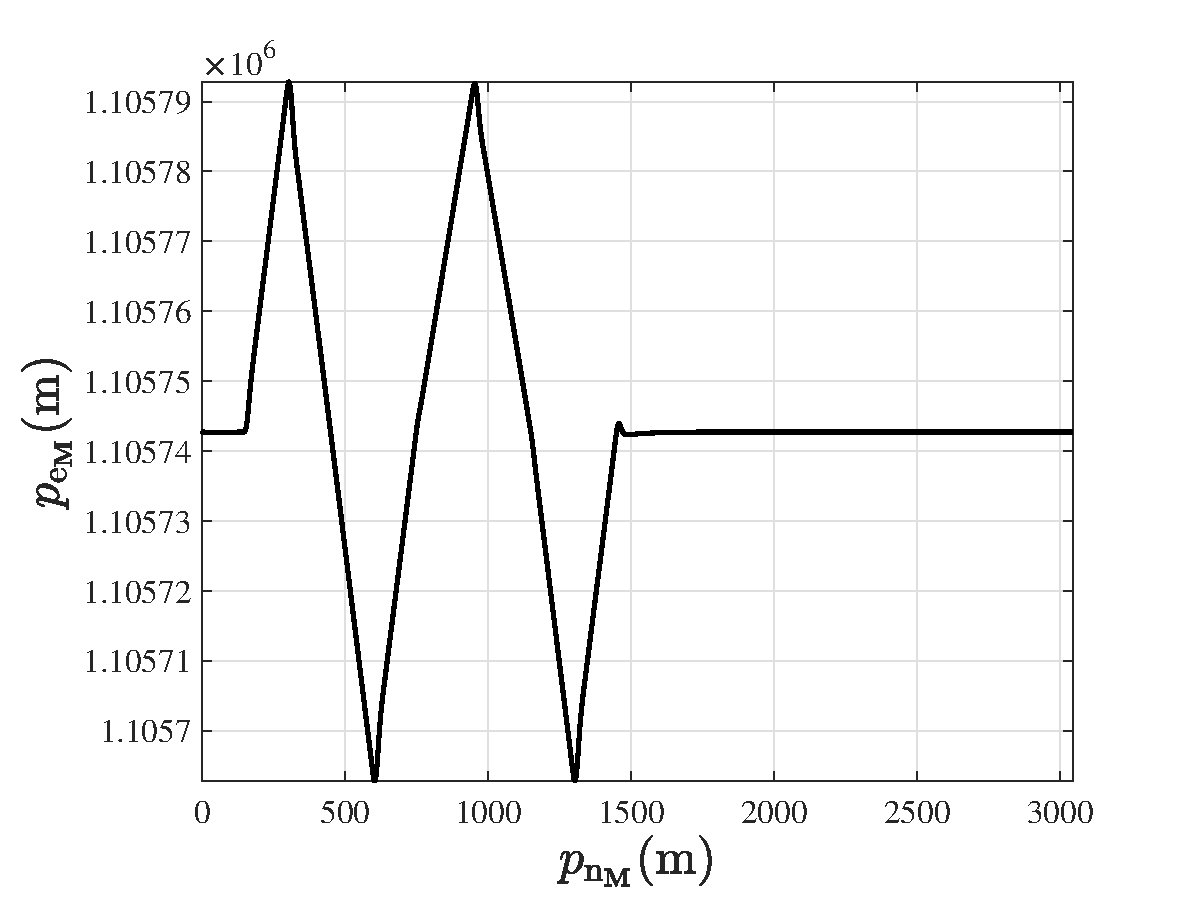
\includegraphics[width=0.5\textwidth]{../Figure/trajectory}
	\caption{Maneuver of the Master Vehicle at Alignment Process}\label{fig:maneuver_TA}
\end{figure}










% In order to asses performance of the proposed technique in real applications, a numerical simulation scenario is designed. As it is mentioned in Section~\ref{sec:problem} there are two mobile platforms named mother carrier and the embedded AUV inside the mother carrier. A commercial USV called Otter was selected to be the mother carrier. Fig~\ref{fig:USVPlatform} shows the Otter USV and its different equipments.
% %\begin{figure}[H]
% %	\centering
% %	% \vspace{0.3cm}
% %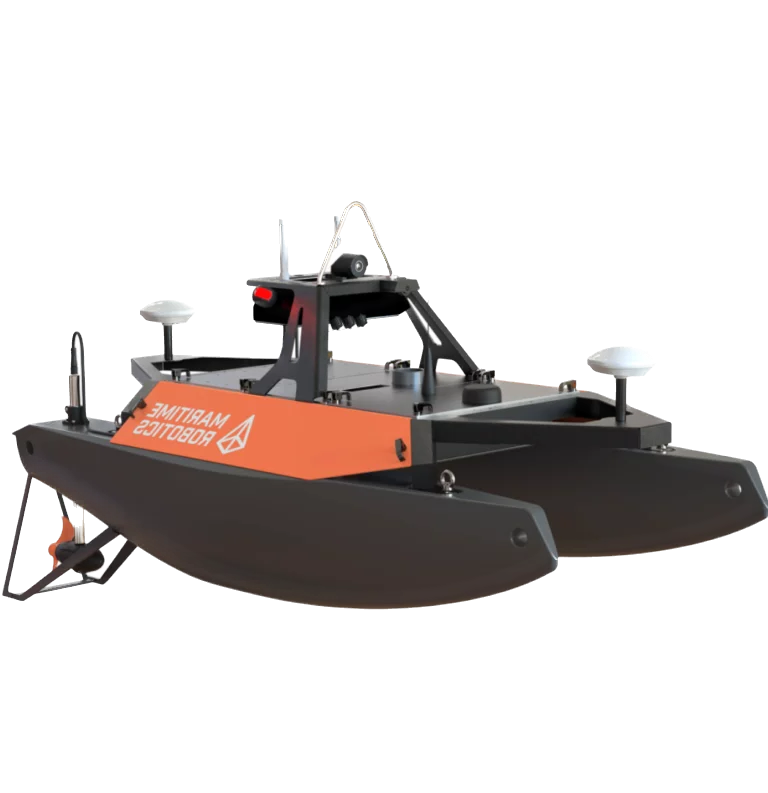
\includegraphics[width=0.5\textwidth]{../Figure/otter.JPG}
% %  \caption{Otter USV as the mother carrier vehicle}
% %  \label{fig:USVPlatform}
% %\end{figure}

% \begin{figure}[H]
% 	\centering
% 	% \vspace{0.3cm}
% \includegraphics[width=0.5\textwidth]{../Figure/Otter.JPG}
%   \caption{The Maritime Robotics Otter Pro USV as the mother carrier vehicle}
%   \label{fig:USVPlatform}
% \end{figure}


% Numerical trajectory simulations were conducted using dynamic equations of the Otter USV at Marine Systems Simulator Simulink toolbox~\cite{fossen2004marine}. It is assumed that the reference navigation system, located on the Otter USV, is a GPS/INS unit with a low-grade MEMS IMU and a conventional GPS . IMU model parameters are reported in Table~\ref{tab:imu_parameters}:

% \begin{table}[H]
%     \renewcommand{\arraystretch}{1.3}
%     \caption{IMU model parameters.}
%     \begin{center}
%         \begin{tabularx}{\textwidth/2}{c X c X c X}
%             \hline
%             Parameter & Value & Parameter & Value & Parameter & Value \\
%             \hline
%             $\mathbf{b}_{a,x}$ & $900\mu g$ & $\mathbf{b}_{a,y}$ & $-1300\mu g$ & $\mathbf{b}_{a,z}$ & $800\mu g$ \\

%             $\mathbf{s}_{a,x}$ & $500\ \text{ppm}$ & $\mathbf{s}_{a,y}$ & $-600\ \text{ppm}$ & $\mathbf{s}_{a,z}$ & $450\ \text{ppm}$ \\

%             $\mathbf{m}_{a,xy}$ & $-300\ \text{ppm}$ & $\mathbf{m}_{a,xz}$ & $200\ \text{ppm}$ & $\mathbf{m}_{a,yz}$ & $250\ \text{ppm}$ \\

%             $\mathbf{m}_{a,yx}$ & $-150\ \text{ppm}$ & $\mathbf{m}_{a,zz}$ & $-250\ \text{ppm}$ & $\mathbf{m}_{a,zy}$ & $100\ \text{ppm}$ \\

%             $\mathbf{b}_{g,x}$ & $-9$ & $\mathbf{b}_{g,y}$ & $13$ & $\mathbf{b}_{g,z}$ & $-8$ \\

%             $\mathbf{s}_{g,x}$ & $1800\ \text{ppm}$ & $\mathbf{s}_{g,y}$ & $-300\ \text{ppm}$ & $\mathbf{s}_{g,z}$ & $-350\ \text{ppm}$ \\

%             $\mathbf{m}_{g,xy}$ & $-300\ \text{ppm}$ & $\mathbf{m}_{g,xz}$ & $250\ \text{ppm}$ & $\mathbf{m}_{g,yz}$ & $-150\ \text{ppm}$ \\
%             \hline
%         \end{tabularx}
%         \label{tab:imu_parameters}
%     \end{center}
% \end{table}

% To observe the heading error and separate the roll and
% pitch errors from the horizontal accelerometer biases, the host vehicle must undergo significant maneuvering, including turns. A linear acceleration or deceleration maneuver couples the heading error into the cross-track velocity and the pitch error into the vertical velocity. Similarly, a turn produces transverse acceleration, which couples the heading error
% into the along-track velocity and the roll error into the vertical velocity~\cite{groves2013principles}. In the simulation scenario, it is assumed that the mother carrier performs a maneuver involving acceleration, deceleration, and turns to align the embedded AUV's INS. Additionally, GPS signals from the reference navigation system are intermittently unavailable during this maneuver.

% Fig~\ref{fig:traj} illustrates that carrier GPS signals are lost during two intervals at the alignment process.

% \begin{figure}[H]
%   \centering
%   \includegraphics[width=0.45\textwidth]{../Figure/LatLon_True.eps}
%   \caption{Mother carrier trajectory (solid) and GNSS outage events (dashed).}
%   \label{fig:traj}
% \end{figure}
% Since the measurement matching phase of the transfer alignment relies on the output solutions of the reference navigation system, the performance of the reference navigation unit during GPS outages is discussed in detail at the following section.
\subsection{Disruption of the GPS Signal}\label{subsec:NN_no}
\noindent In this section, the performance of the robust in-motion transfer alignment algorithm is investigated, when the GPS information outages. For this purpose, the interruption of the GPS signal takes 755 seconds (between 1045 \& 1800 seconds).

\subsubsection{Performance of the Master Navigation Unit}
\noindent The Fig~\ref{fig:maneuver_TA} shows the trajectory of the boat (with and without GPS).
Moreover, the results of the master navigation unit performance is evaluated in Fig~\ref{fig:master_no_ai}, when GPS outages.
It can be observed that the state errors increase significantly, when the GPS signal is interrupted during the specific interval (1045 to 1800 seconds).
% \hl{After acquiring GPS, the master navigation algorithm experiences a transient response in the boat's velocity. This change causes to increase the attitude errors of the boat.}
Consequently, the performance of the master navigation algorithm is disrupted.
%%%%%%%%%%%%%% fig %%%%%%%%%%%%%%%
% \begin{figure}[H]
% 	\centering
% 	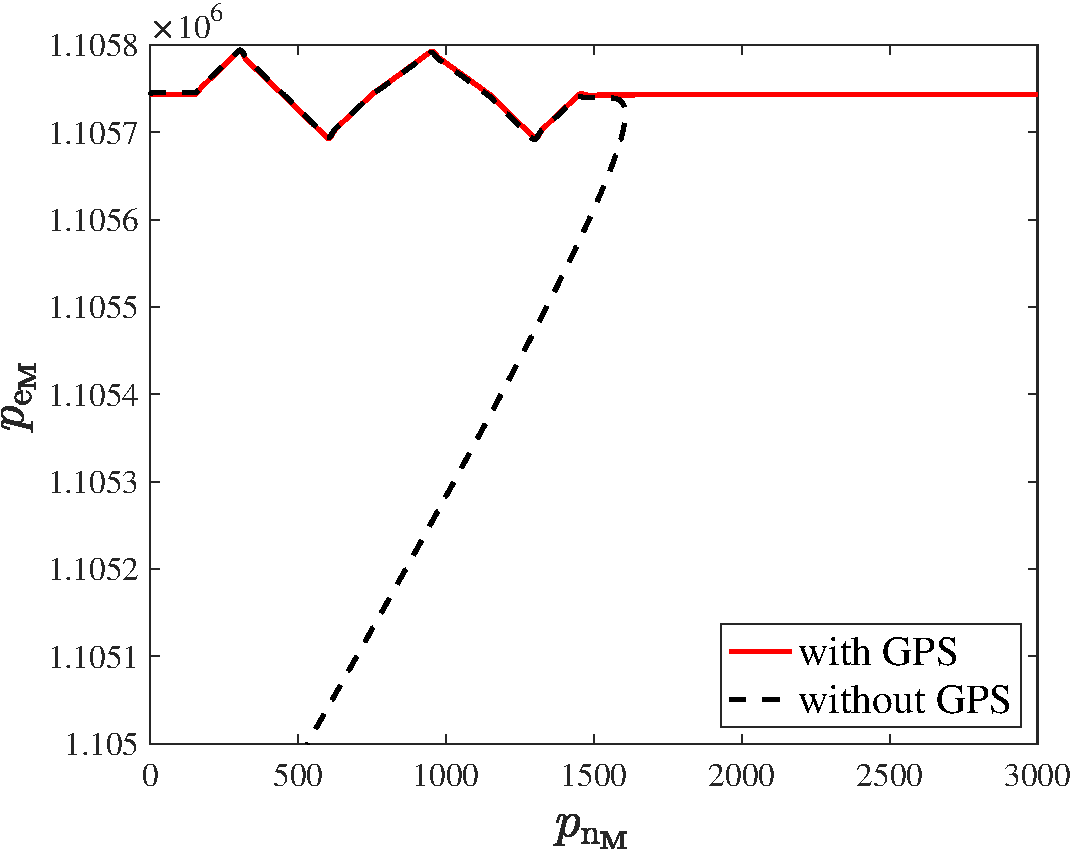
\includegraphics[width=0.45\textwidth]{../Figure/AI-results/trajectory}
% 	\caption{Trajectory of Master Vehicle, When GPS Outages}\label{fig:trajectory}
% \end{figure}
\begin{figure}[H]
	\centering
	% \vspace{0.3cm}
	\subfloat[\label{fig:PN}]{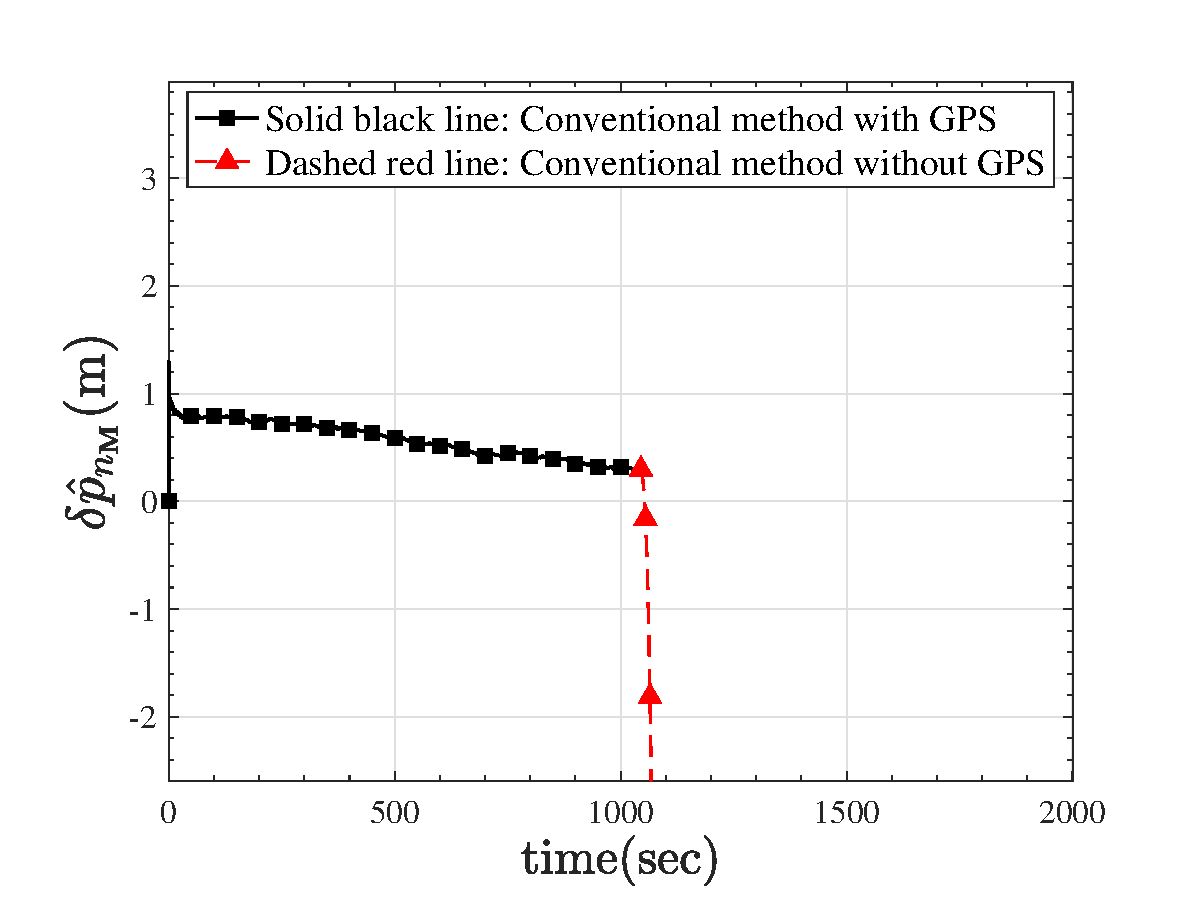
\includegraphics[width=.33\textwidth]{../Figure/AI-results/Master/North position error}{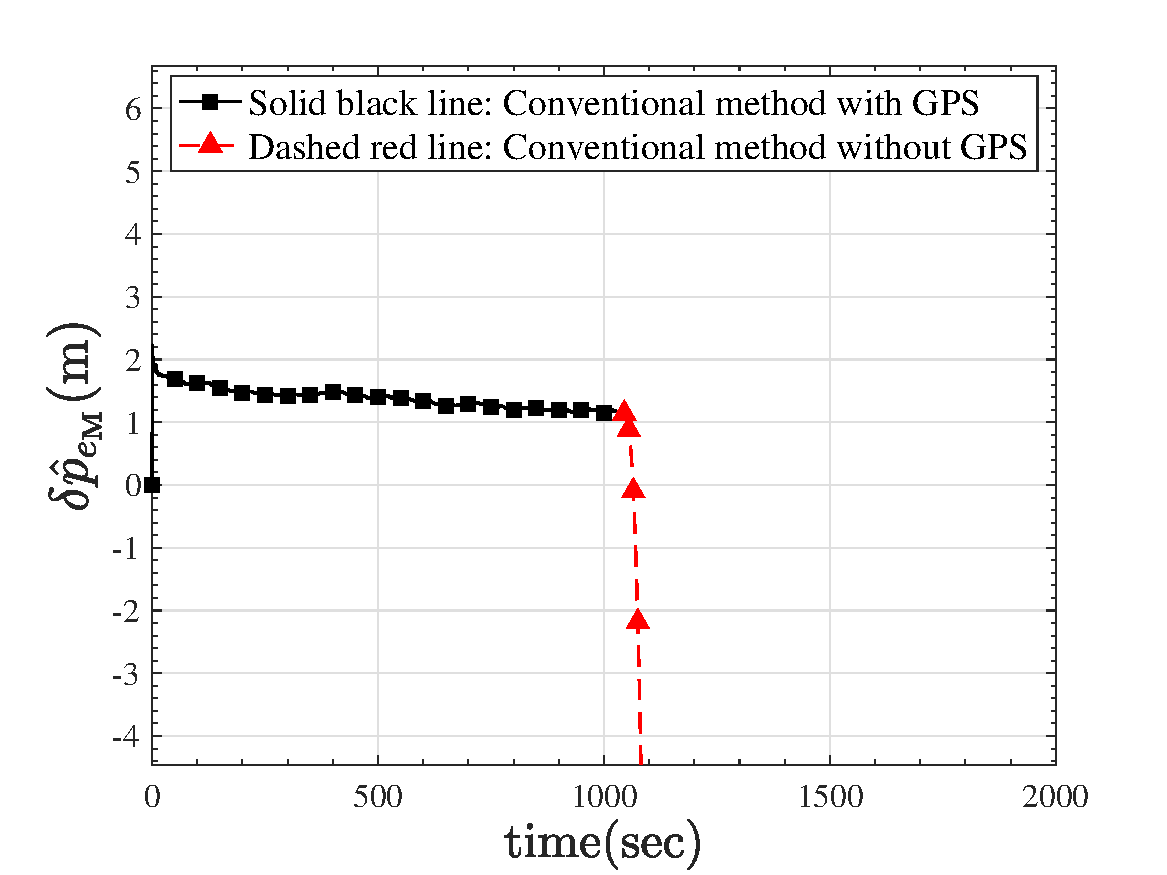
\includegraphics[width=.33\textwidth]{../Figure/AI-results/Master/East position error}
	{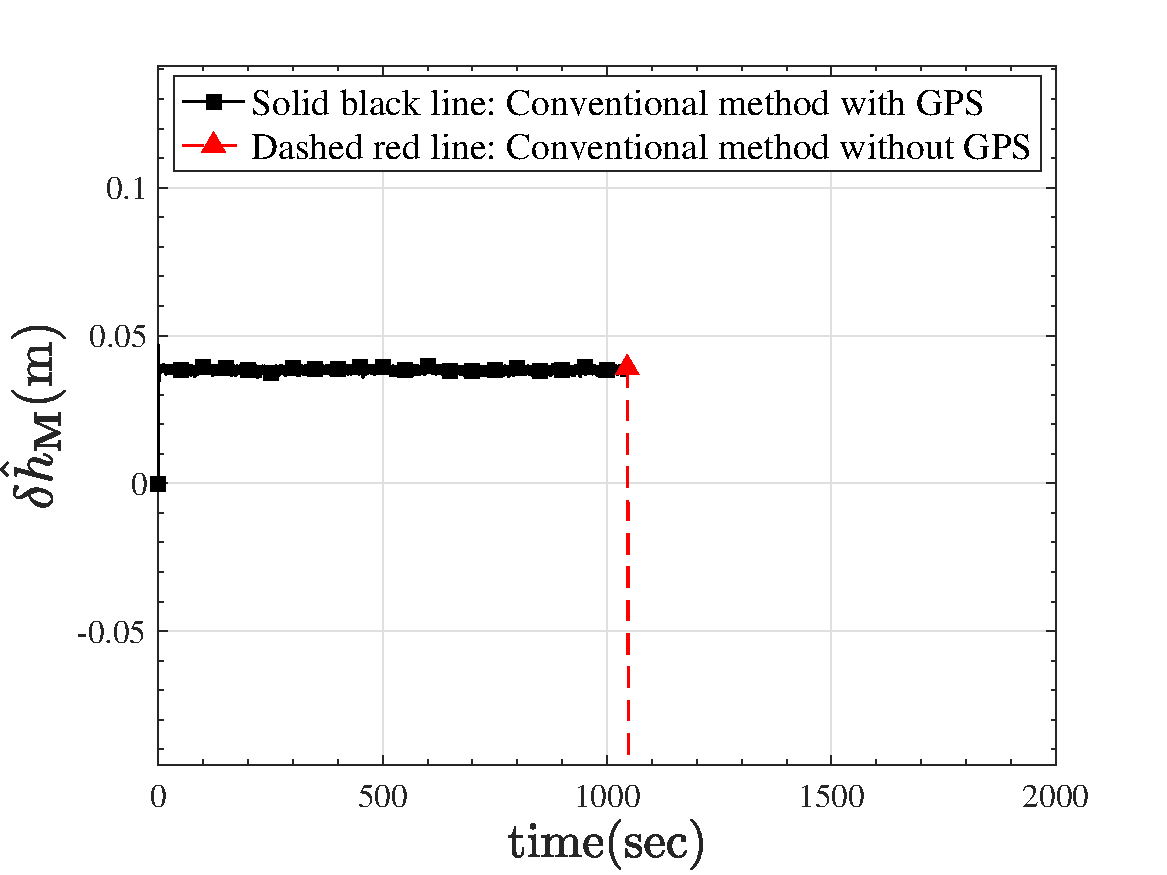
\includegraphics[width=.33\textwidth]{../Figure/AI-results/Master/Down position error}}}
	}\\
	\subfloat[\label{fig:VN}]{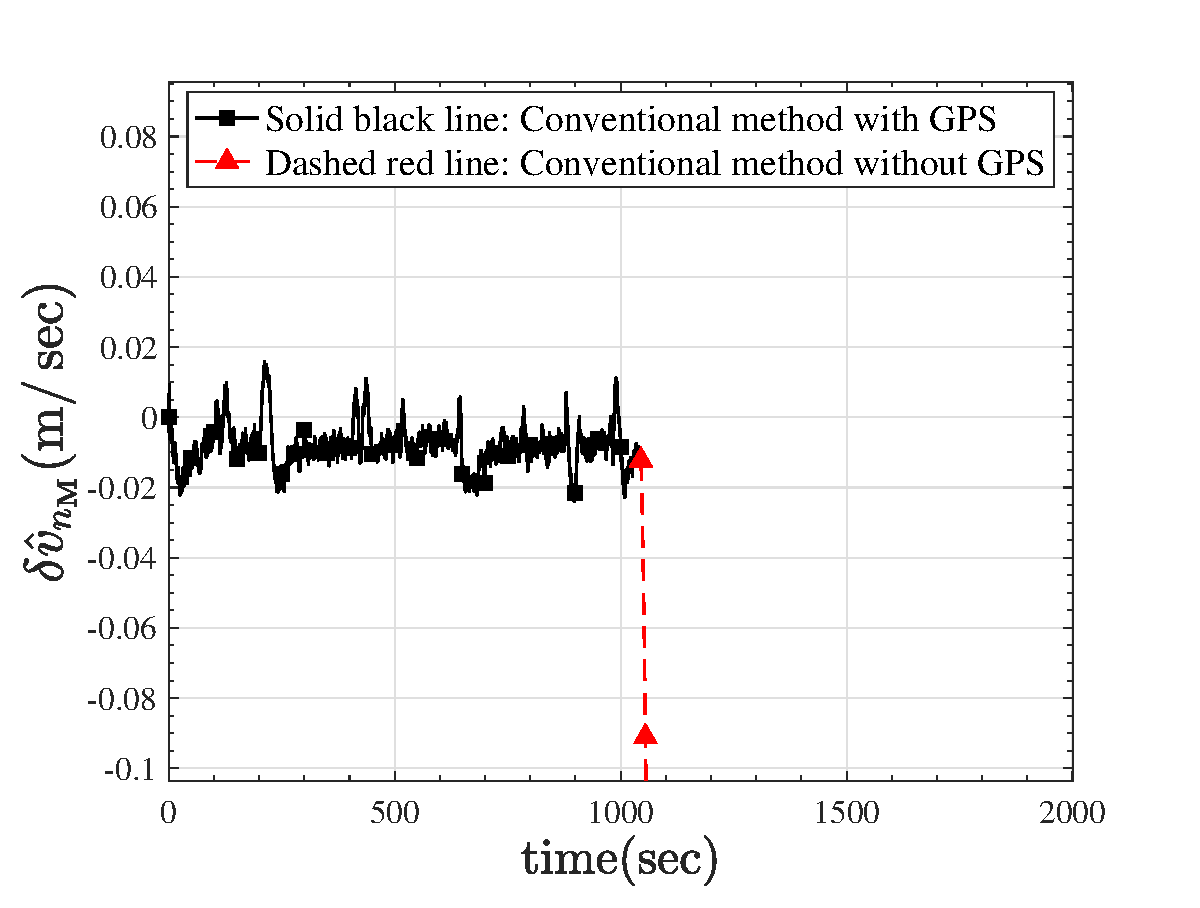
\includegraphics[width=.33\textwidth]{../Figure/AI-results/Master/North velocity error}{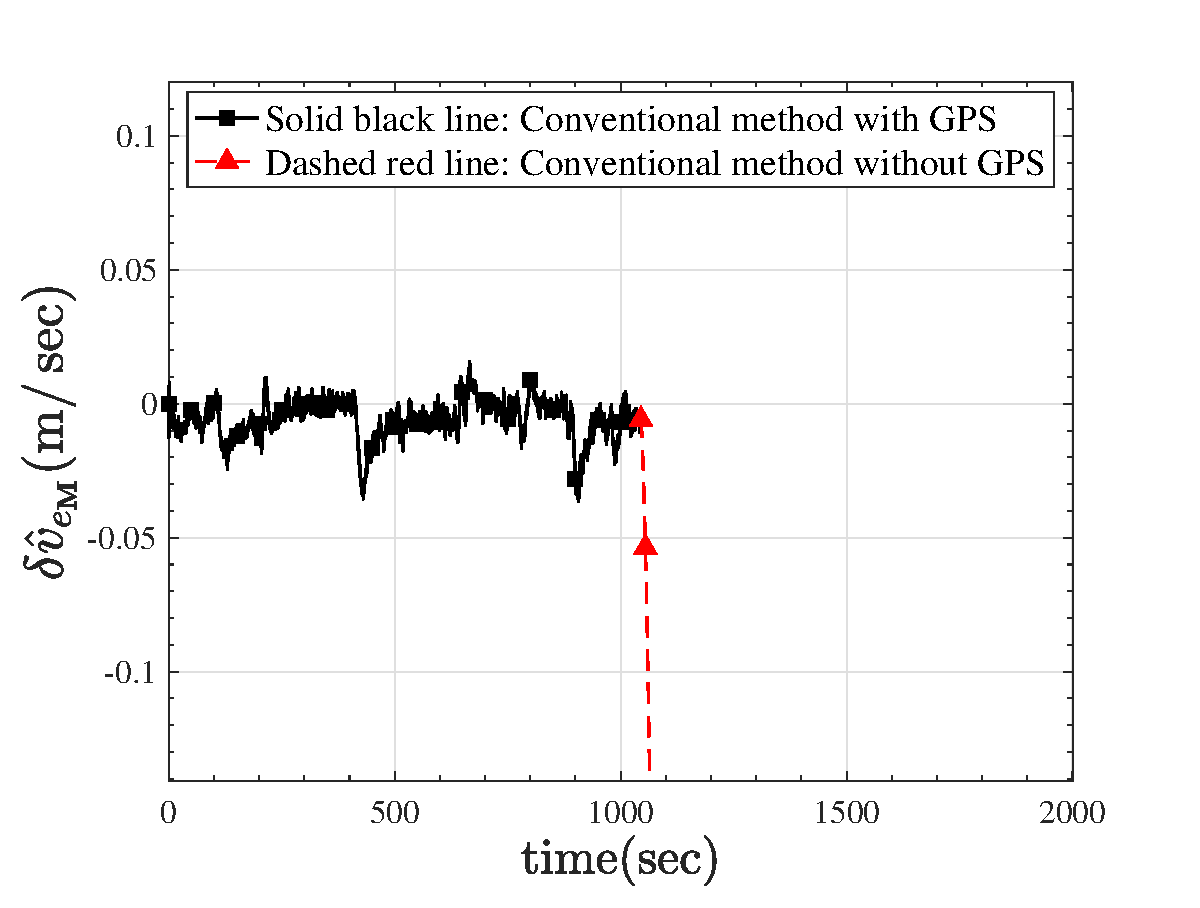
\includegraphics[width=.33\textwidth]{../Figure/AI-results/Master/East velocity error}
	{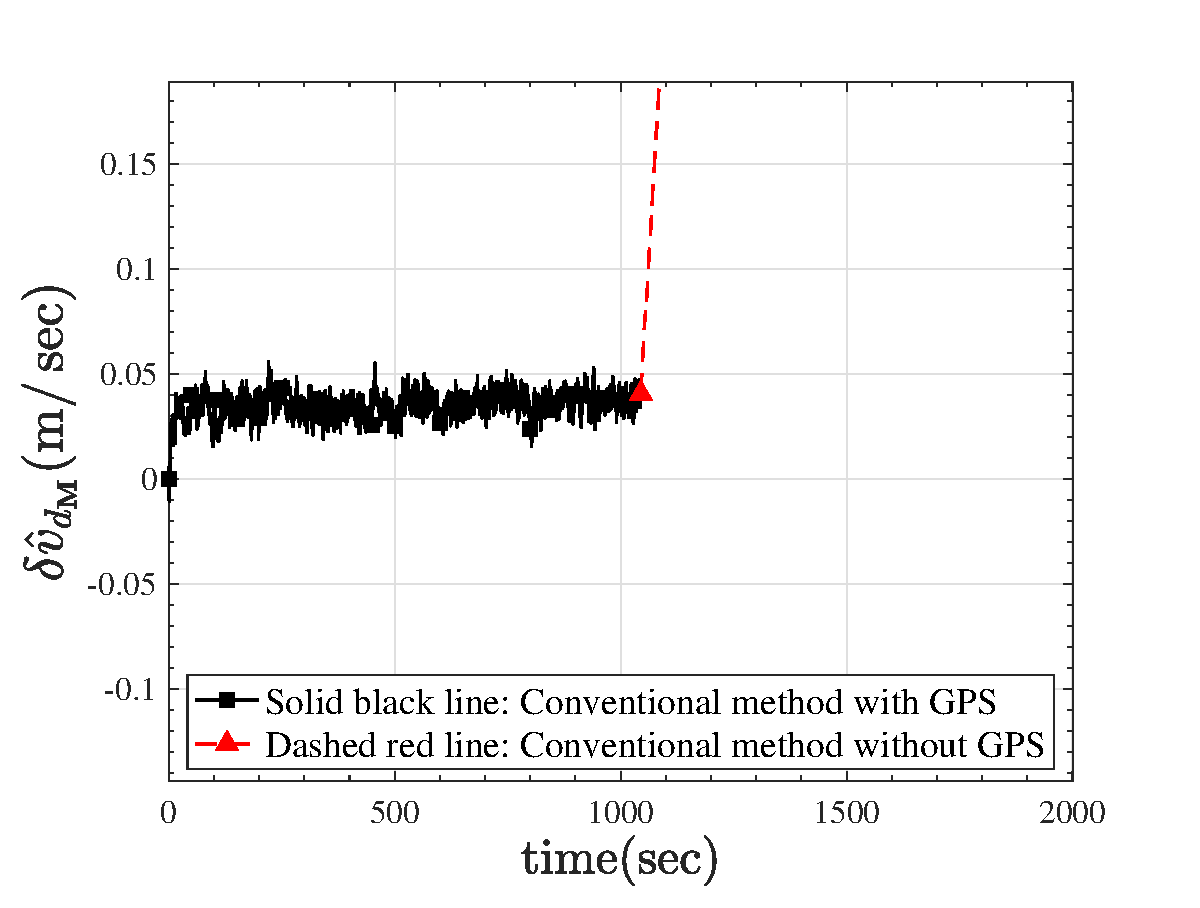
\includegraphics[width=.33\textwidth]{../Figure/AI-results/Master/Down velocity error}}}
	}\\
	\subfloat[\label{fig:AN}]{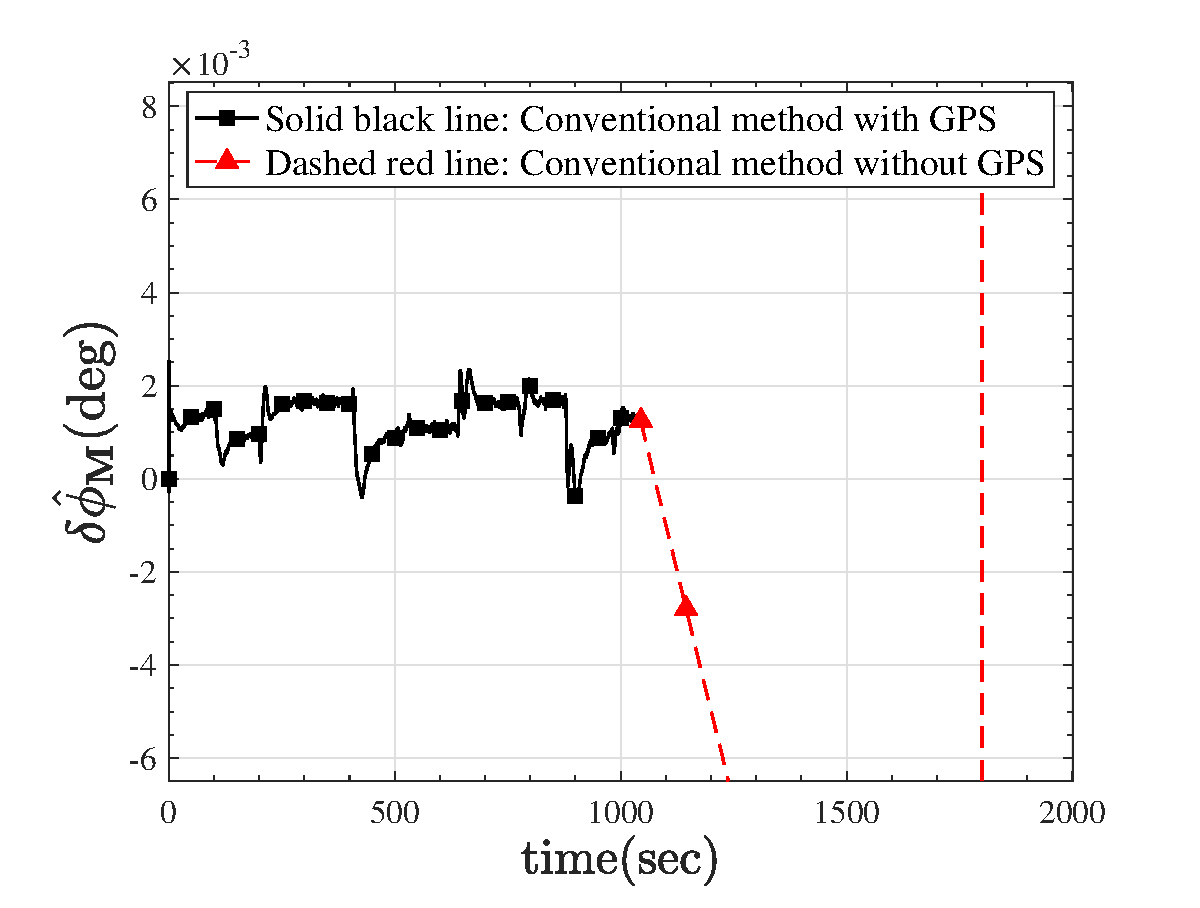
\includegraphics[width=.33\textwidth]{../Figure/AI-results/Master/Attitude error about North}{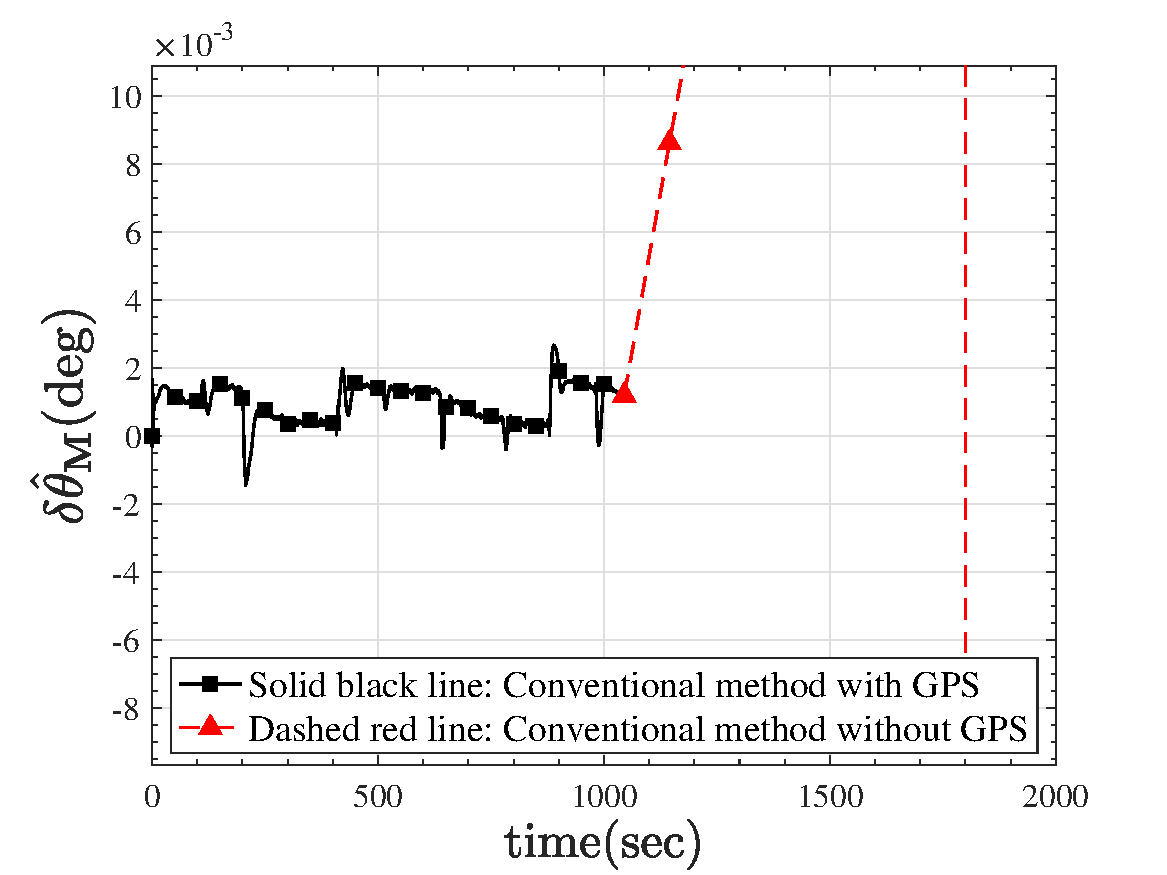
\includegraphics[width=.33\textwidth]{../Figure/AI-results/Master/Attitude error about East}
	{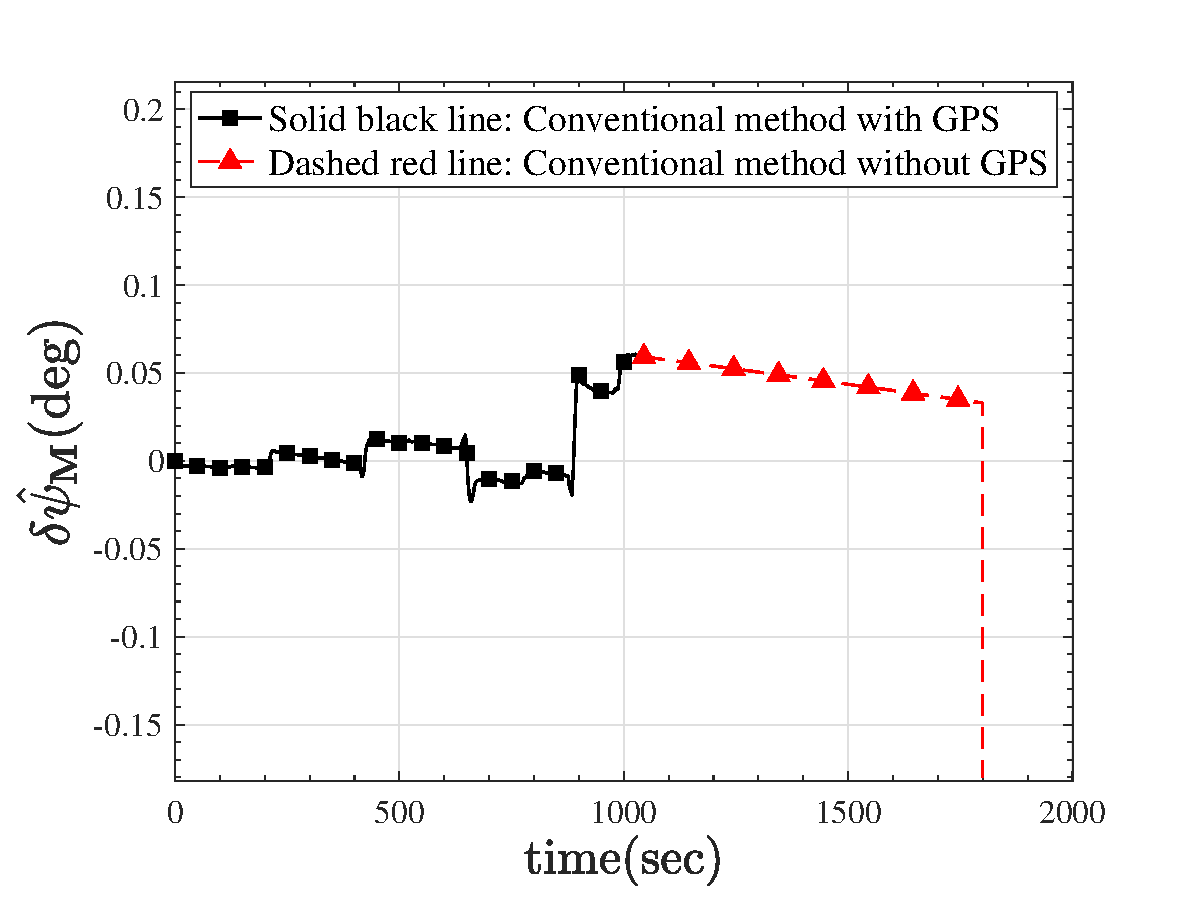
\includegraphics[width=.33\textwidth]{../Figure/AI-results/Master/Heading error}}}
	}
	\caption{%
% Performance of the Master Navigation Algorithm when GPS signals are lost.
% In each plot, the line changes at the point of GPS outage to highlight
% the transition from GPS-based to inertial-only navigation.
% Position error~\ref{sub@fig:PN},
% Velocity error~\ref{sub@fig:VN},
% Attitude error~\ref{sub@fig:AN}.
Performance comparison of the Master Navigation Algorithm: Conventional method with GPS (Solid line) vs. Conventional method without GPS (Dashed red line):~\ref{sub@fig:PN} Position error (m),~\ref{sub@fig:VN} Velocity error (m/\(\sec\)),~\ref{sub@fig:AN} Attitude error (\(\deg\)).
}\label{fig:master_no_ai}
\end{figure}

















\subsubsection{Performance of Slave Navigation Unit}
\noindent Here, transfer alignment algorithm performance is evaluated in Fig~\ref{fig:slave}~\ref{sub@fig:SPN} to~\ref{fig:slave}~\ref{sub@fig:SAN}, when the GPS of the master unit outages.
This figure shows the state errors including the errors of the position (\(\delta \hat{\mathbf{p}}_{\mathbf{S}}\)), velocity (\(\delta \hat{\mathbf{v}}_{\mathbf{S}}\)), and attitude (\(\delta \hat{\mathbf{a}}_{\mathbf{S}}\)) of the slave vehicle. When the GPS signal is available
 the proposed approach can estimate the true states of the slave vehicle properly. However, the transfer alignment algorithm does not work correctly, when the GPS signals are disrupted and not available in some times.


\begin{figure}[H]
	\centering
	% \vspace{0.3cm}
	\subfloat[\label{fig:SPN}]{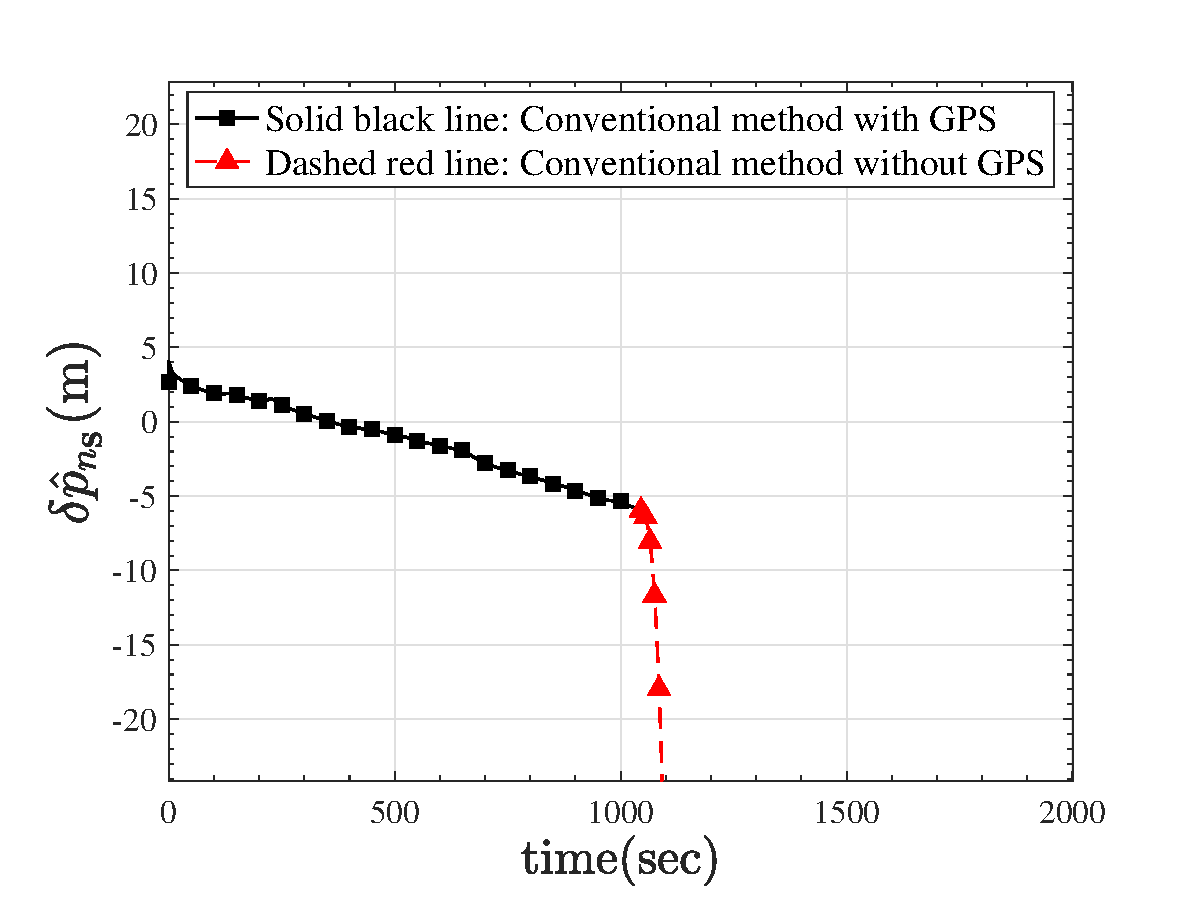
\includegraphics[width=.33\textwidth]{../Figure/AI-results/Slave/North position error}{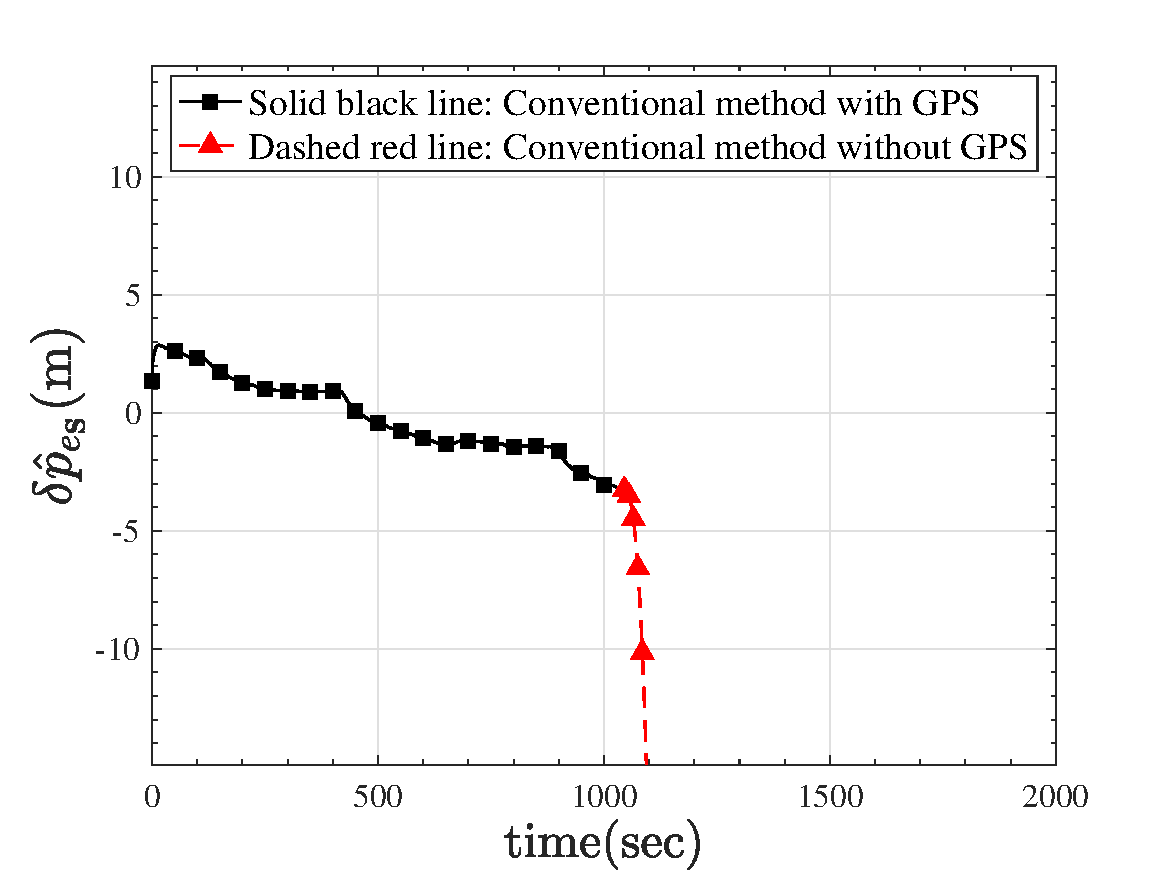
\includegraphics[width=.33\textwidth]{../Figure/AI-results/Slave/East position error}
	{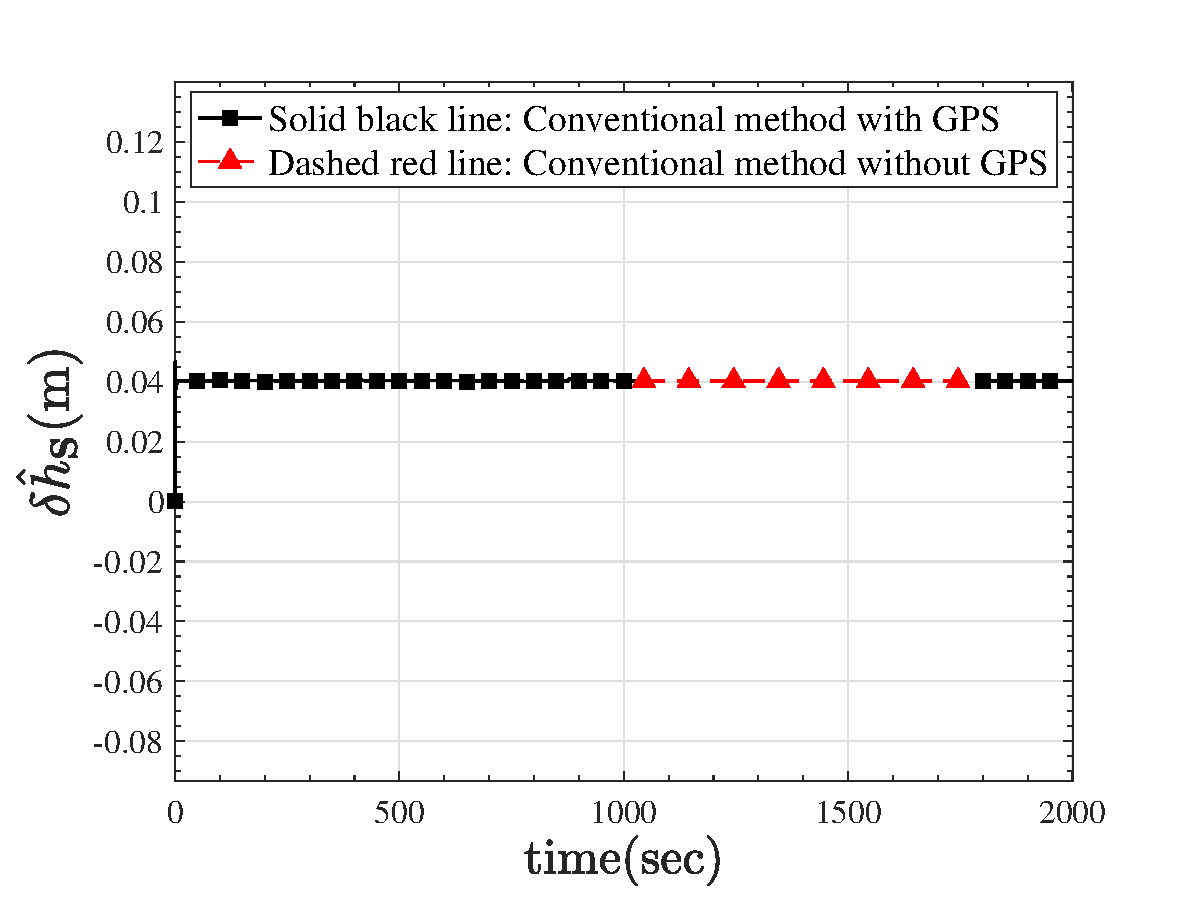
\includegraphics[width=.33\textwidth]{../Figure/AI-results/Slave/Down position error}}}
	}\\
	\subfloat[\label{fig:SVN}]{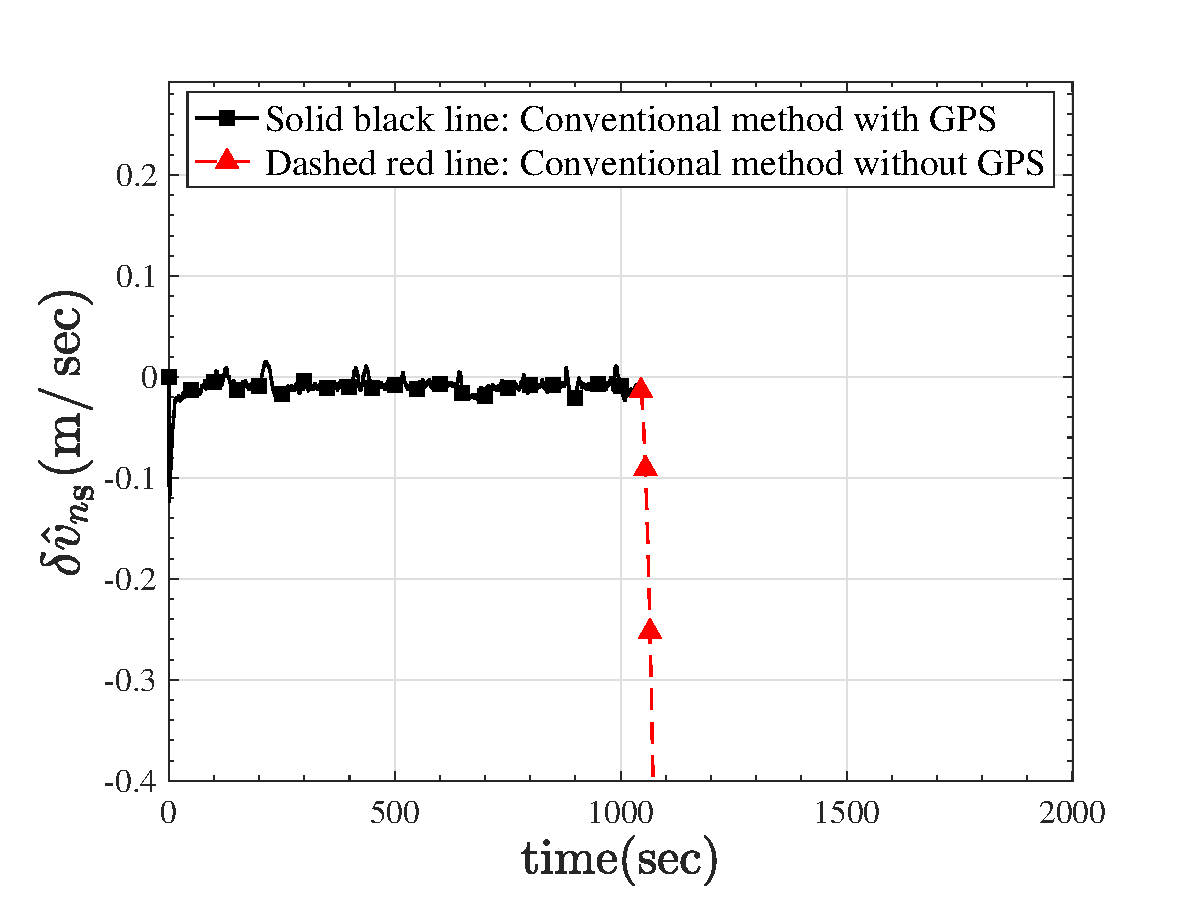
\includegraphics[width=.33\textwidth]{../Figure/AI-results/Slave/North velocity error}{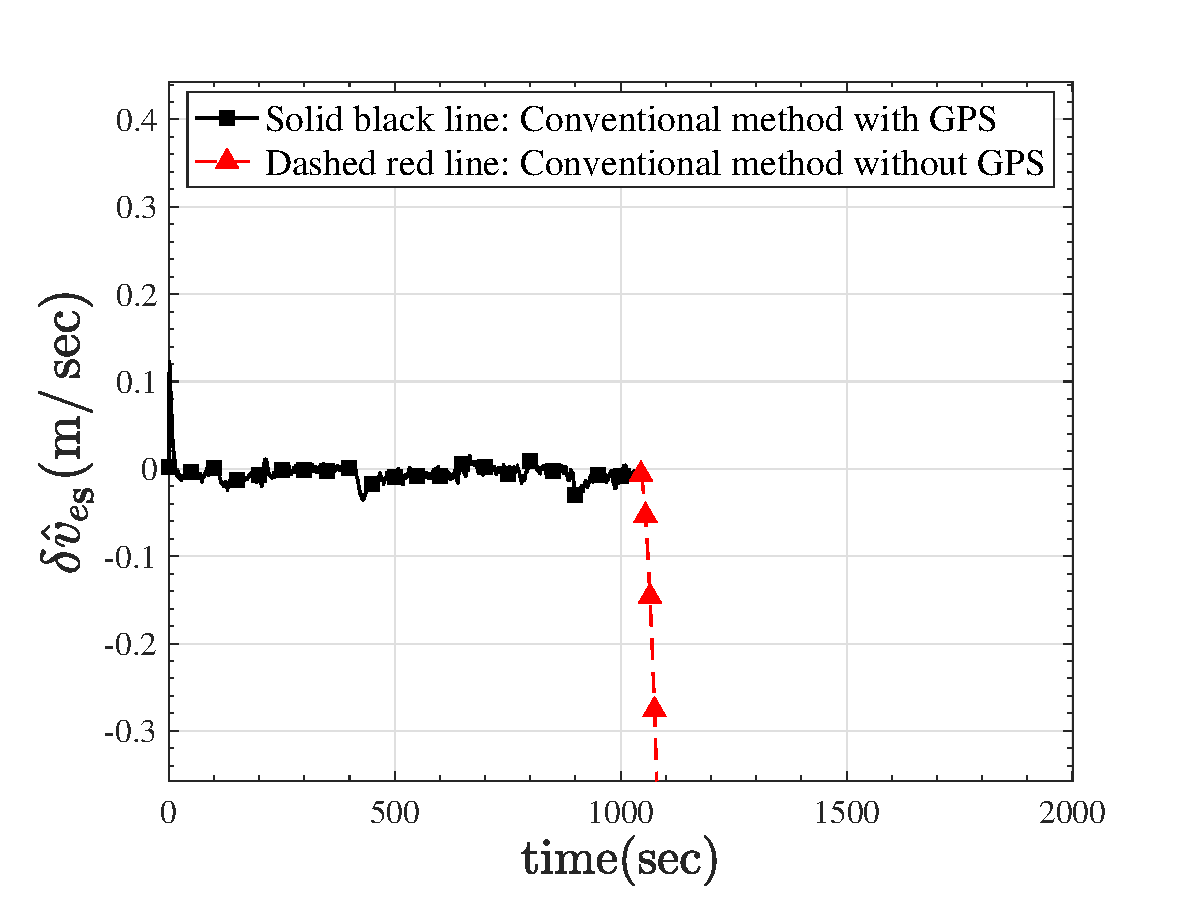
\includegraphics[width=.33\textwidth]{../Figure/AI-results/Slave/East velocity error}
	{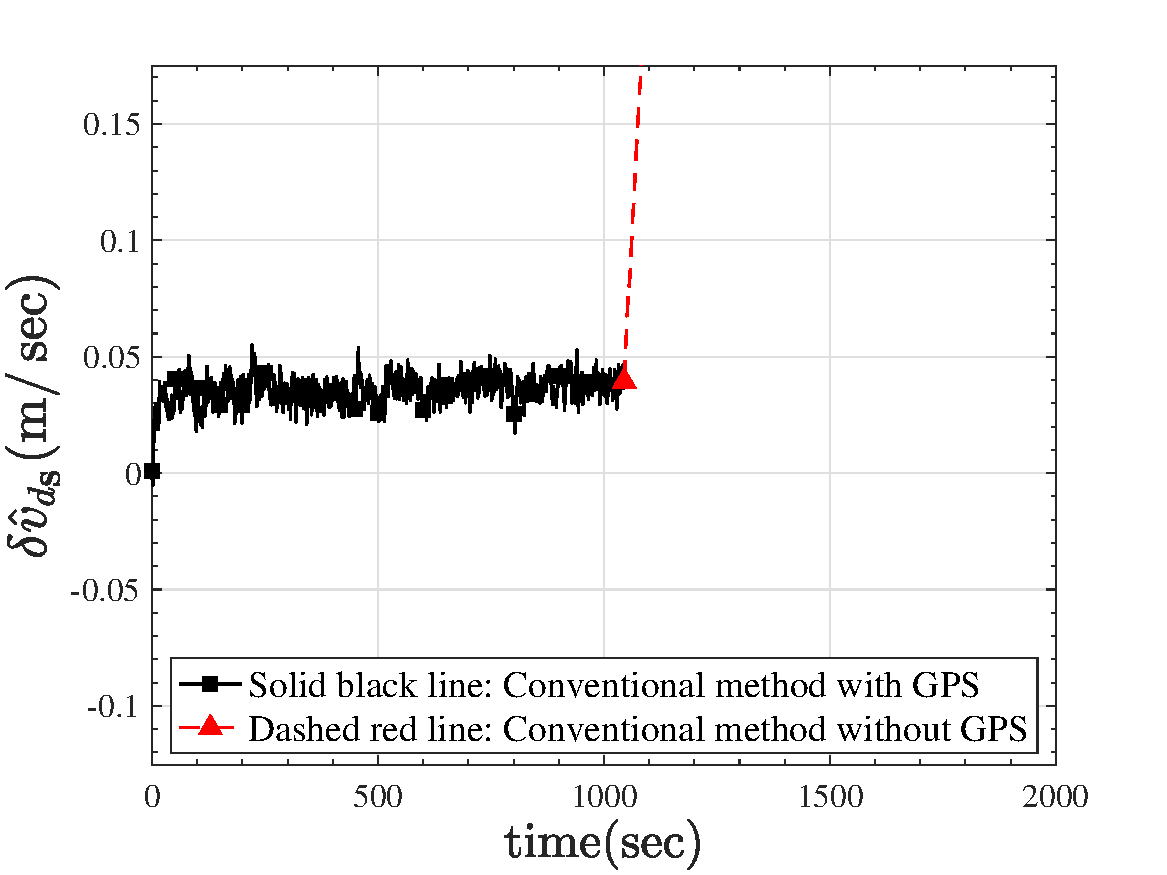
\includegraphics[width=.33\textwidth]{../Figure/AI-results/Slave/Down velocity error}}}
	}\\
	\subfloat[\label{fig:SAN}]{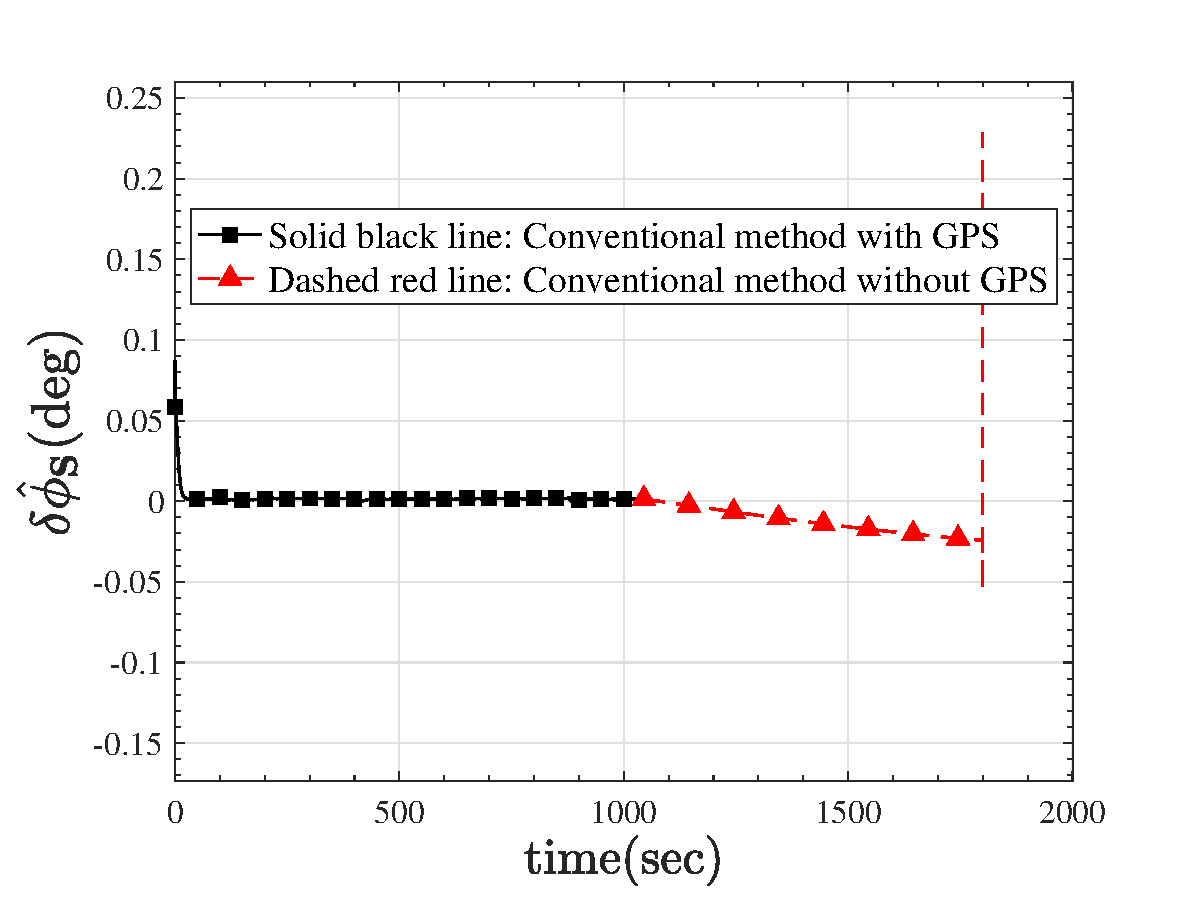
\includegraphics[width=.33\textwidth]{../Figure/AI-results/Slave/Attitude error about North}{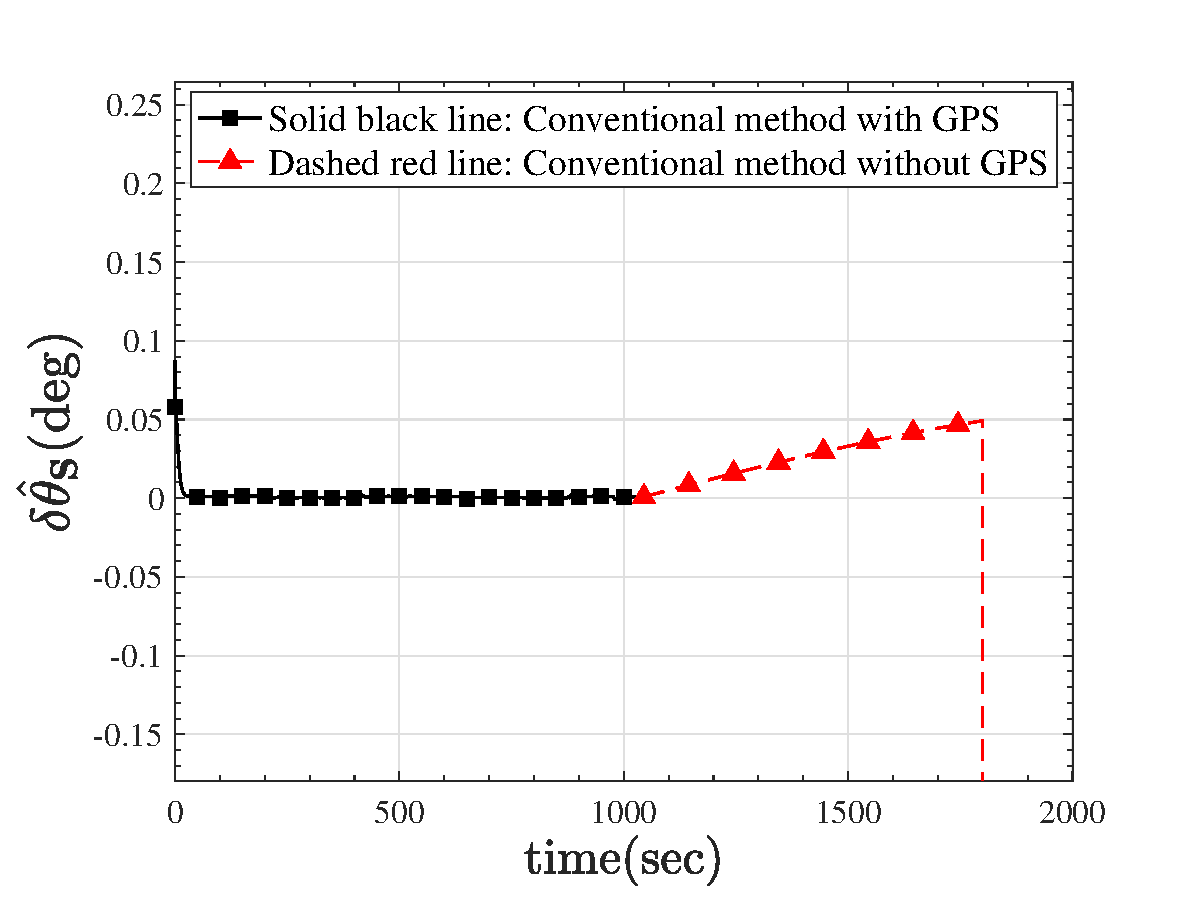
\includegraphics[width=.33\textwidth]{../Figure/AI-results/Slave/Attitude error about East}
	{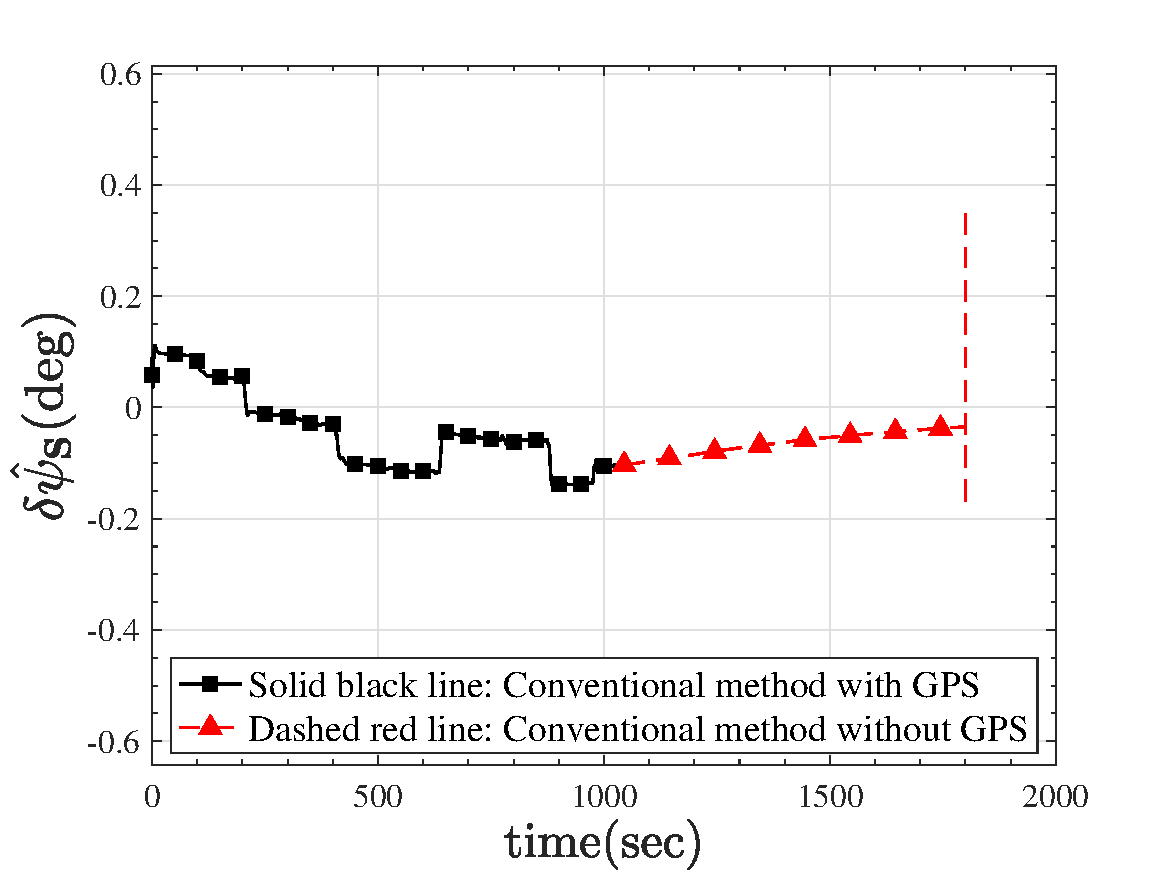
\includegraphics[width=.33\textwidth]{../Figure/AI-results/Slave/Heading error}}}
	}
	\caption{%
% Performance of the Slave Navigation Algorithm when GPS signals are lost.
% In each plot, the line changes at the point of GPS outage to highlight the transition 
% from GPS-based to inertial-only navigation. 
% Position error~\ref{sub@fig:SPN}, 
% velocity error~\ref{sub@fig:SVN}, 
% and attitude error~\ref{sub@fig:SAN}.%
Performance comparison of the Slave Navigation Algorithm: Conventional method with GPS (Solid line) vs. Conventional method without GPS (Dashed red line):~\ref{sub@fig:SPN} Position error (m),~\ref{sub@fig:SVN} Velocity error (m/\(\sec\)),~\ref{sub@fig:SAN} Attitude error (\(\deg\)).
}
	\label{fig:slave}
\end{figure}















\subsection{Performance of Proposed NN}\label{subsec:NN_used}
\noindent Here, the results of the training and prediction phases of the proposed model are presented, when GPS signal of the master navigation unit is disrupted. For this purpose, first, the training of the NN model is discussed. Then, the performance of the master and slave vehicles are investigated.

\subsubsection{Training of the Neural Network Model}
\noindent The training of the proposed NN model is performed using the sequential data of the master's IMU and SINS outputs.
For this purpose, the Adam optimizer~\cite{kingma2014adam} is employed to increase the efficiency and robustness in training phase of deep model.
%  A learning rate of 0.001 is chosen to balance the convergence speed and stability of the training process.
% The model undergoes training for a total of 100 epochs.
%  This number of epochs is selected based on preliminary experiments to ensure that the model sufficiently learns the underlying patterns in the data without overfitting. During training, both the training and validation losses are monitored to evaluate the model's performance and generalization ability.
Then, the training process was conducted on the Google Colab platform, utilizing the computational power of an NVIDIA T4 GPU\@.
% , which significantly accelerated the training process.
The specifications of the training phase are denoted in Table~\ref{tab:training}.
 Moreover, the training and validation losses are shown in Fig~\ref{fig:loss}.
 It is observed that the trained model is effectively learned from the data, as the loss values consistently decrease throughout the training process.
%  A consistent decrease, indicating that the model is effectively learning from the data.
% The final trained model achieves a minimum loss of 0.0001, which demonstrates the model's capability to closely predict the target outputs.

%  The complete training duration is recorded to be approximately 1 hour, 2 minutes, and 6 seconds. This time includes all epochs and the necessary computations, highlighting the efficiency of the proposed training setup.

% table %
% \begin{table}[H]
% 	\centering
% 	\caption{
% 		Charachteristic of the Training Phase of the Porposed NN
% 	}
% 	\begin{tabular}{|c|c|}
% 		\hline
% 		\textbf{Aspect} & \textbf{Specification} \\
% 		\hline
% 		Optimizer & Adam \\
% 		Learning Rate & 0.001 \\
% 		Epochs & 100 \\
% 		Hardware Used & NVIDIA T4 GPU \\
% 		Training Time & 1 hour, 2 minutes, 6 seconds \\
% 		\hline
% 	\end{tabular}
% 	\label{tab:training}
% \end{table}
\normalsize
\begin{table}[H]
	\centering
	\caption{
		Characteristics of the Training Phase of the Proposed NN
	}
	\begin{tabular}{l|l}
		\hline
		\textbf{Aspect} & \textbf{Specification} \\
		\hline
		Training Algorithm & Adam Optimizer \\
		Learning Rate & 0.001 \\
		Number of Epochs & 100 \\
		Hardware & NVIDIA T4 GPU \\
		Total Training Time & 1 hour, 2 minutes, 6 seconds \\
		\hline
	\end{tabular}\label{tab:training}
\end{table}



\begin{figure}[H]
	\centering
	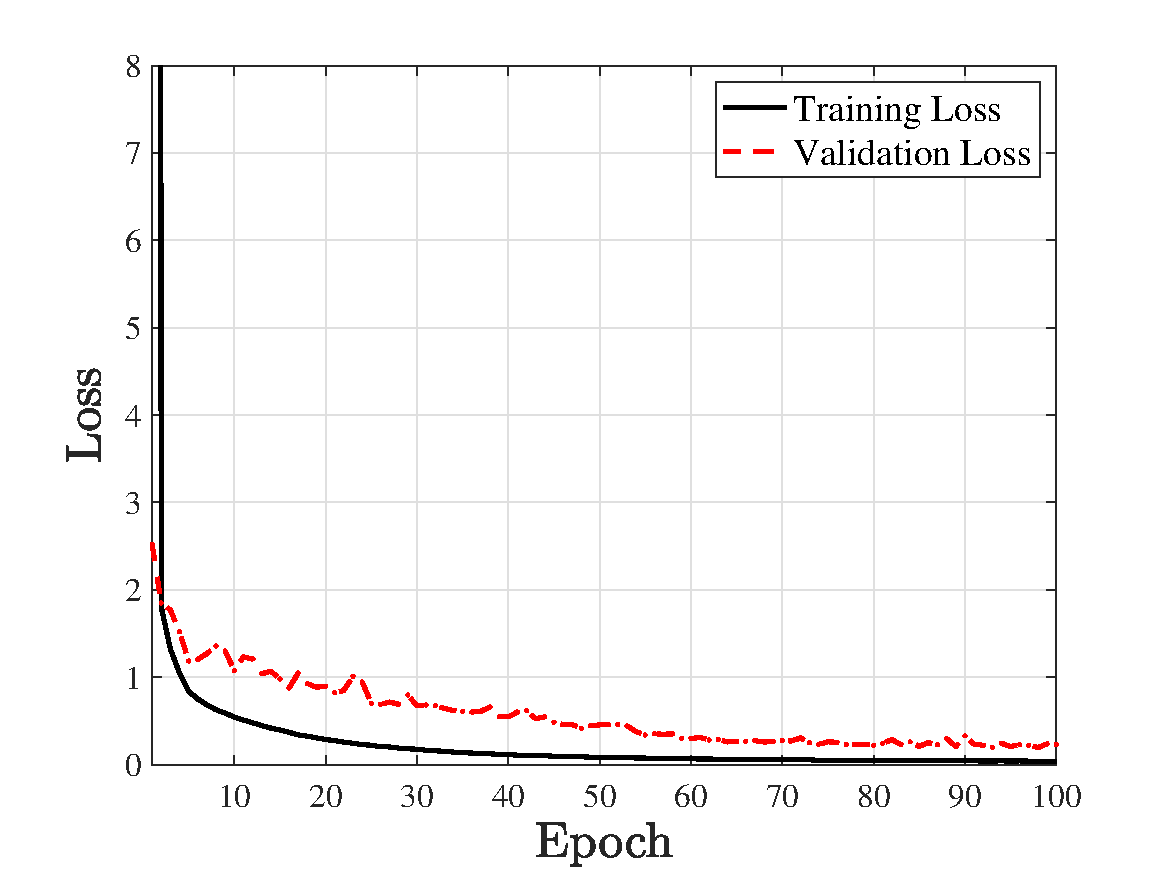
\includegraphics[width=0.45\textwidth]{../Figure/loss}
	\caption{Training and Validation Loss of the Proposed NN Model}\label{fig:loss}
\end{figure}


\subsubsection{Performance of Master Navigation Unit}
\noindent Here, the results of the master navigation unit is evaluated in Fig~\ref{fig:AI_master}. It can be observed that the state errors do not increase significantly using the proposed NN,
when the GPS signal interrupted during the specific interval (1045 \& 1800 seconds).

\begin{figure}[H]
	\centering
	% \vspace{0.3cm}
	\subfloat[\label{fig:MPN_AI}]{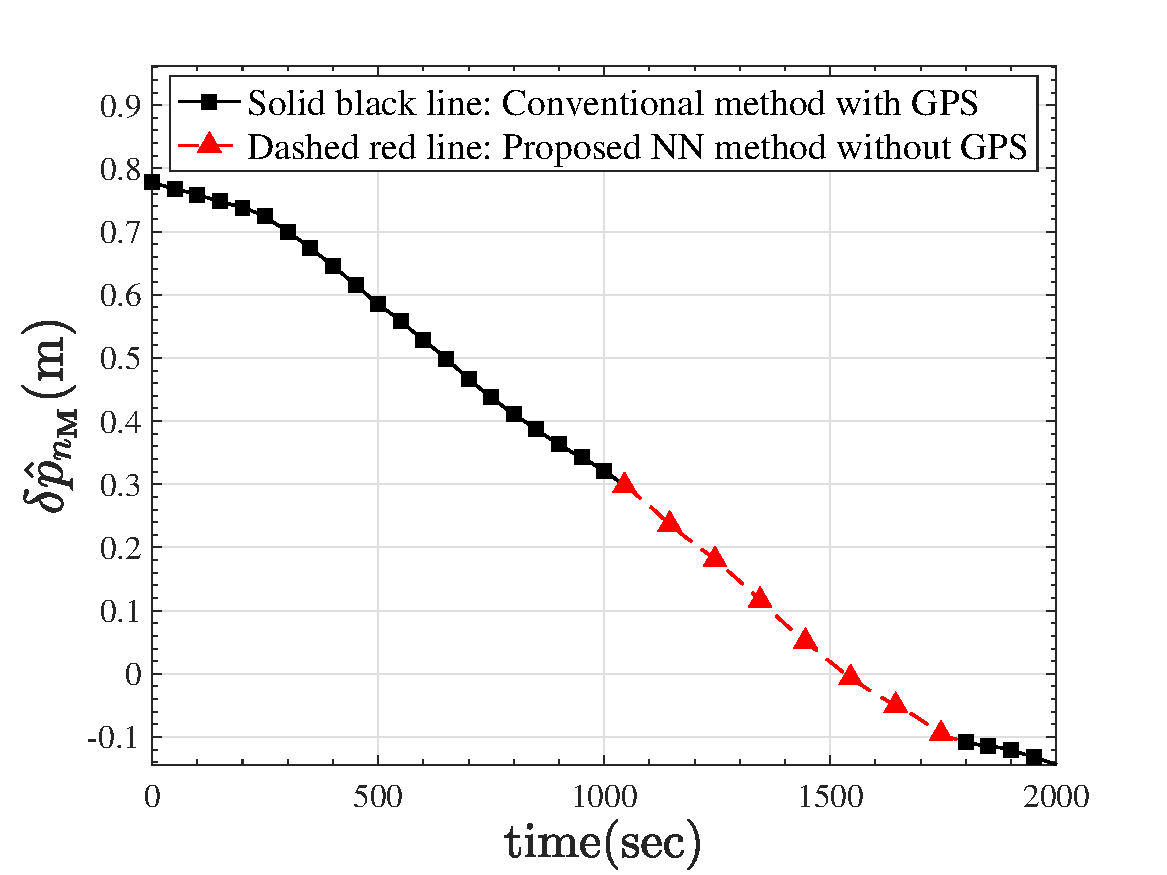
\includegraphics[width=.33\textwidth]{../Figure/AI-results/Master/North position errorAI}{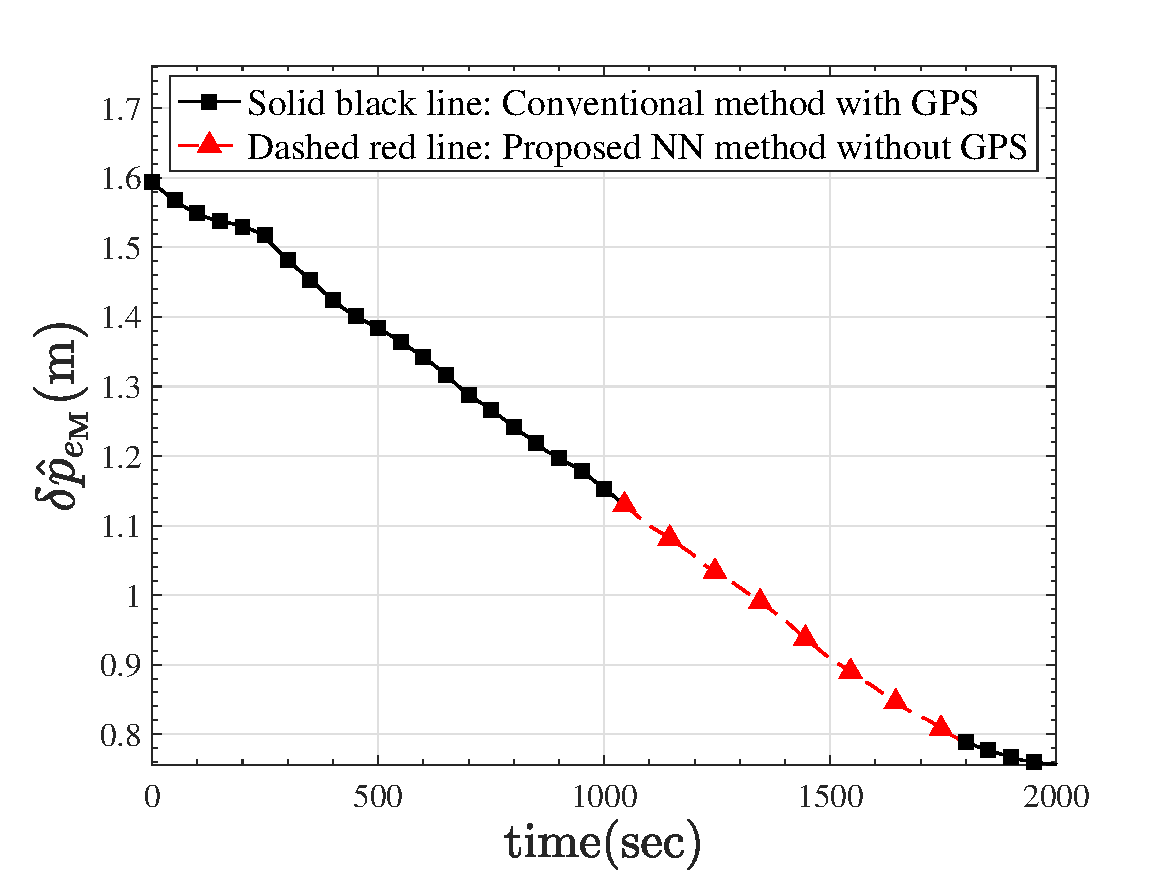
\includegraphics[width=.33\textwidth]{../Figure/AI-results/Master/East position errorAI}
	{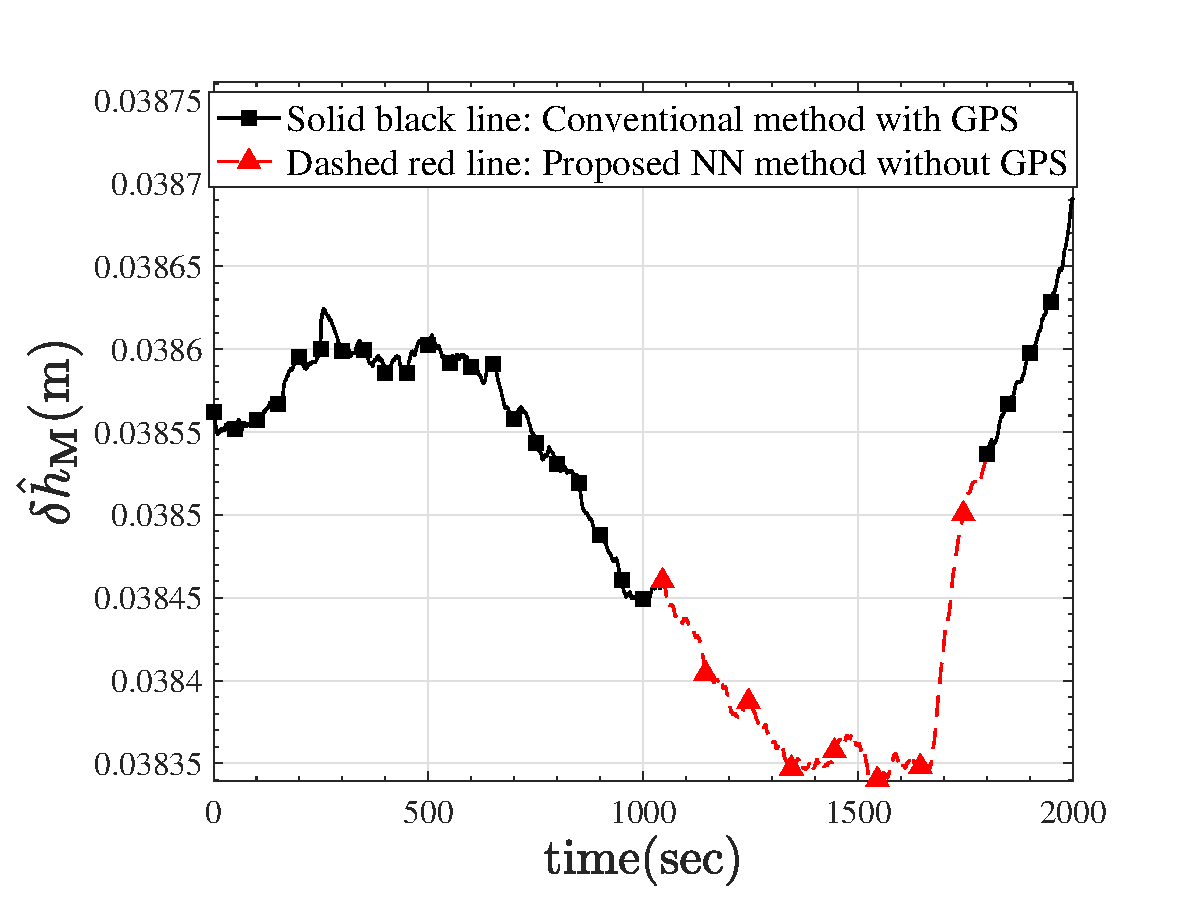
\includegraphics[width=.33\textwidth]{../Figure/AI-results/Master/Down position errorAI}}}
	}\\
	\subfloat[\label{fig:MVN_AI}]{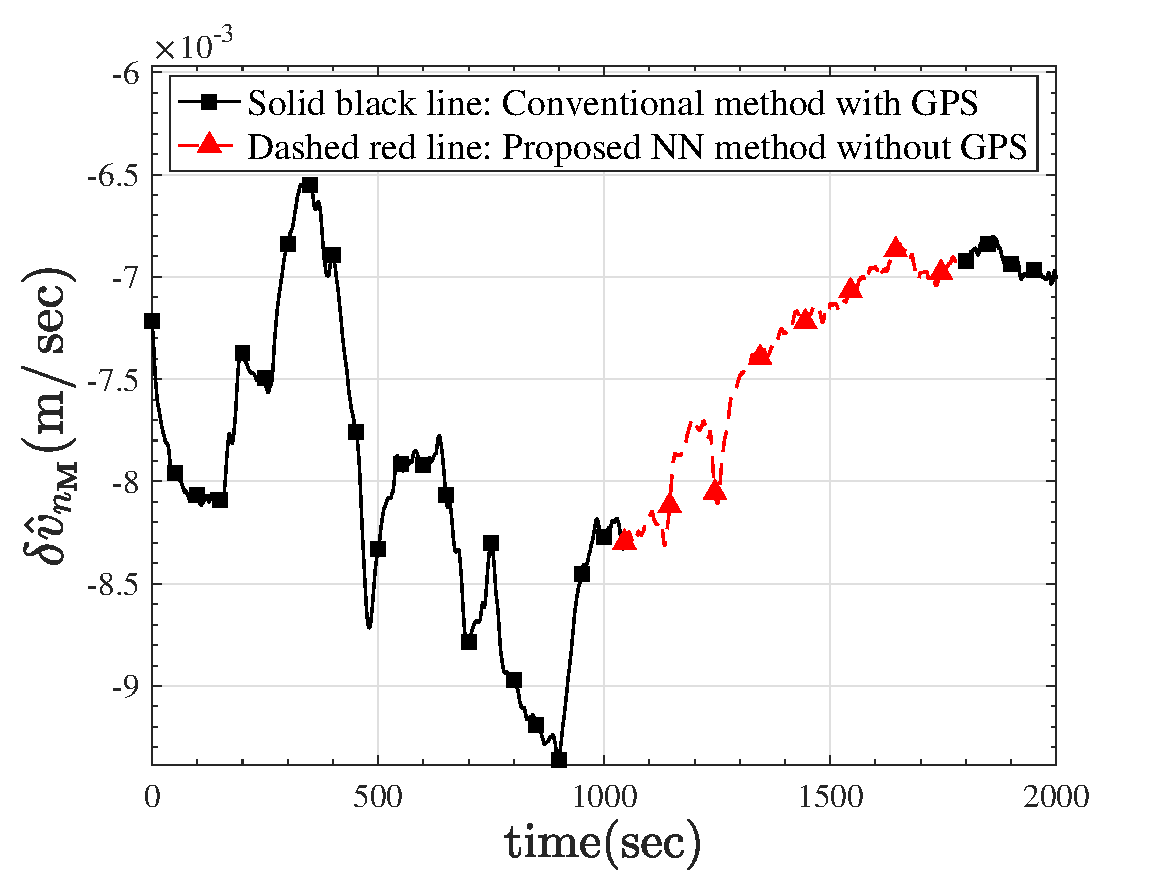
\includegraphics[width=.33\textwidth]{../Figure/AI-results/Master/North velocity errorAI}{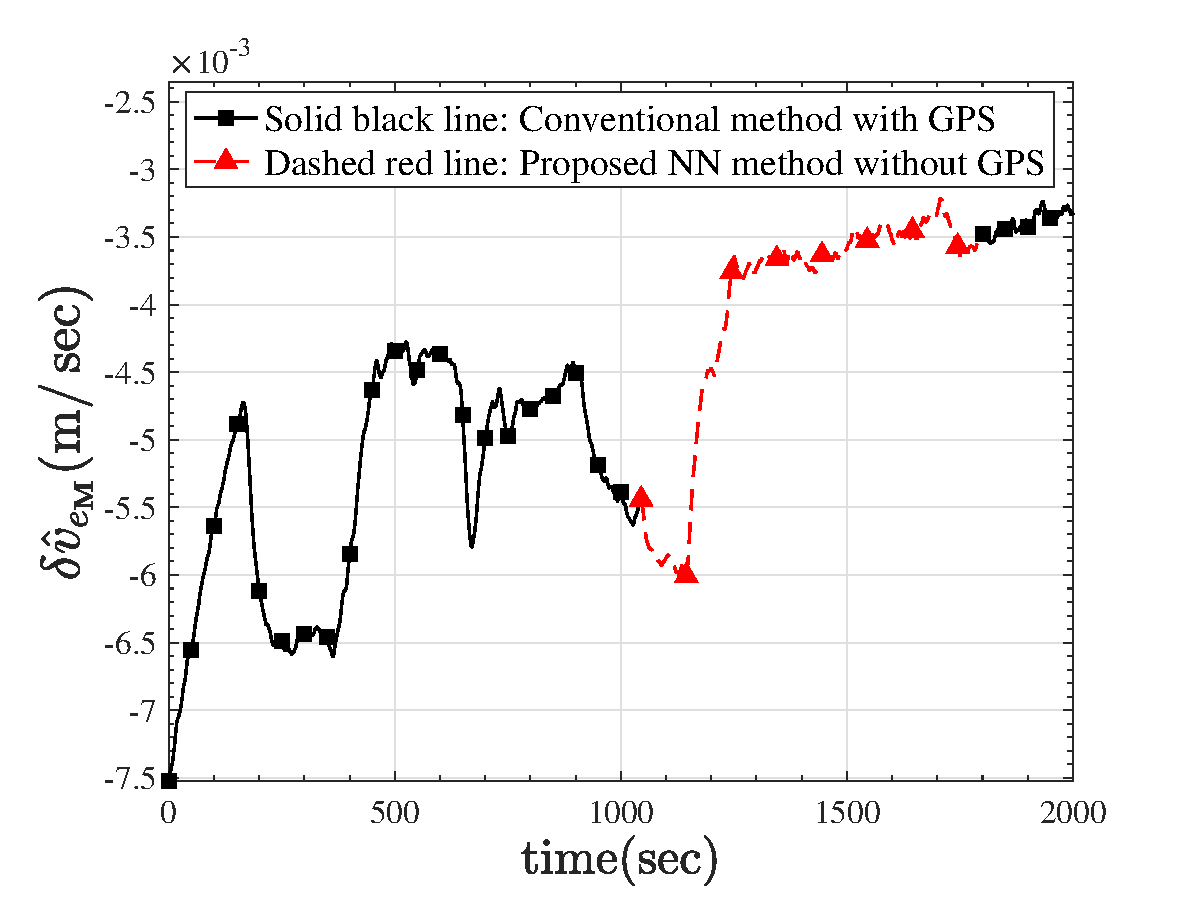
\includegraphics[width=.33\textwidth]{../Figure/AI-results/Master/East velocity errorAI}
	{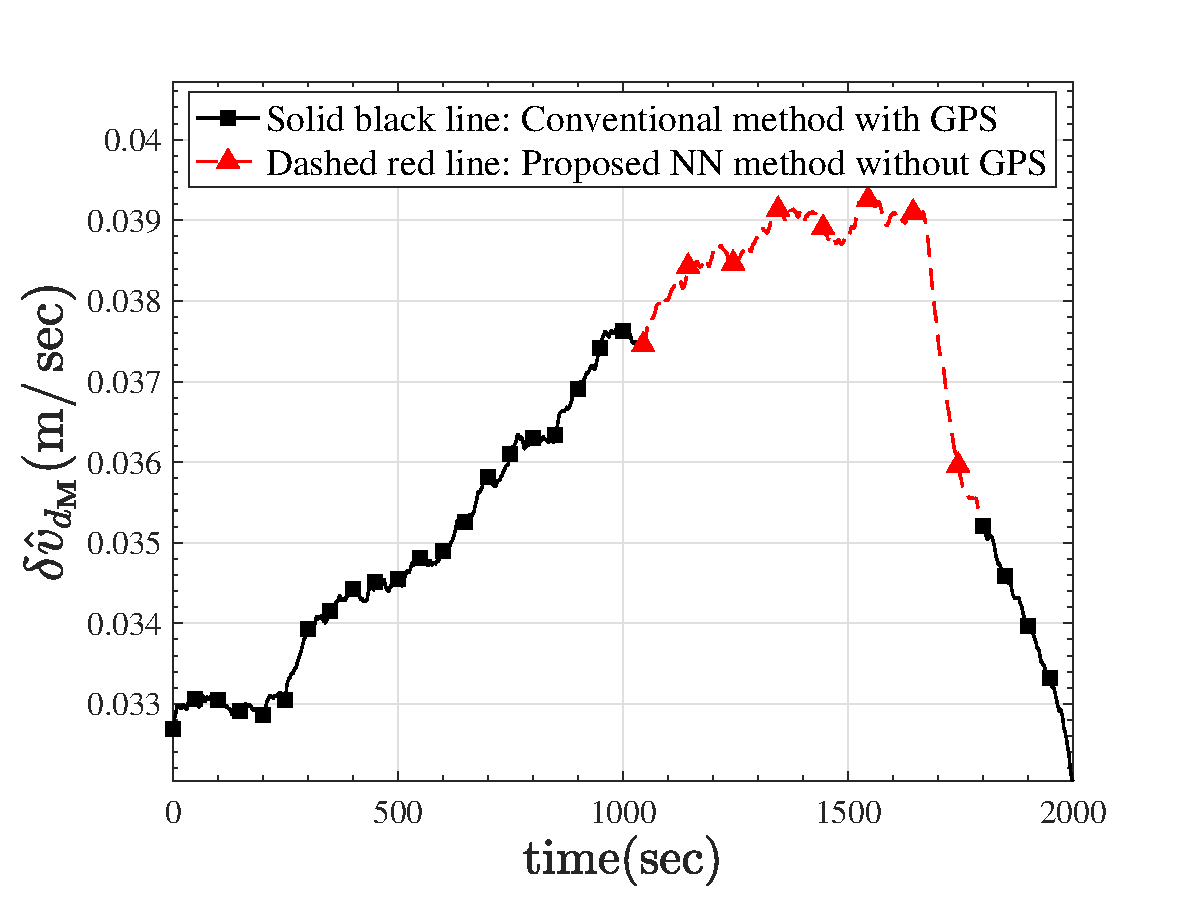
\includegraphics[width=.33\textwidth]{../Figure/AI-results/Master/Down velocity errorAI}}}
	}\\
	\subfloat[\label{fig:MAN_AI}]{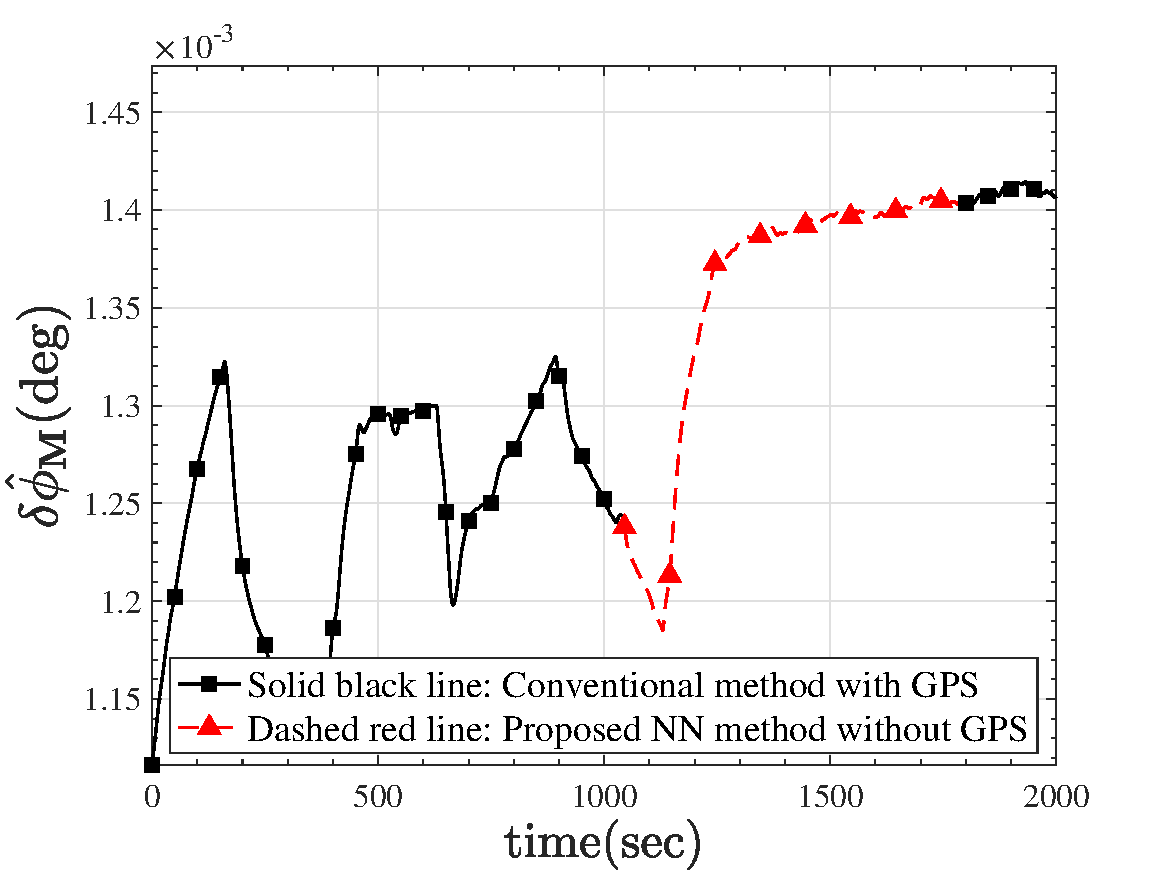
\includegraphics[width=.33\textwidth]{../Figure/AI-results/Master/Attitude error about NorthAI}{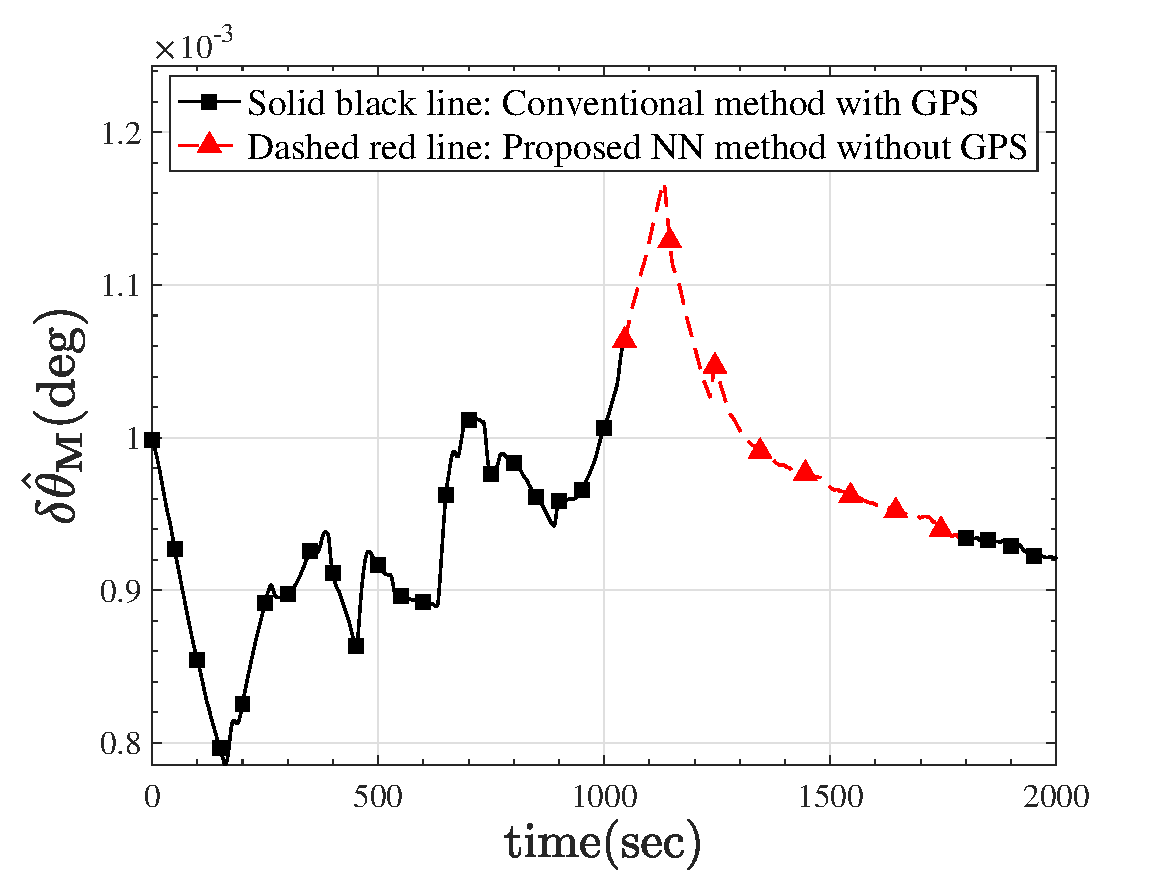
\includegraphics[width=.33\textwidth]{../Figure/AI-results/Master/Attitude error about EastAI}
	{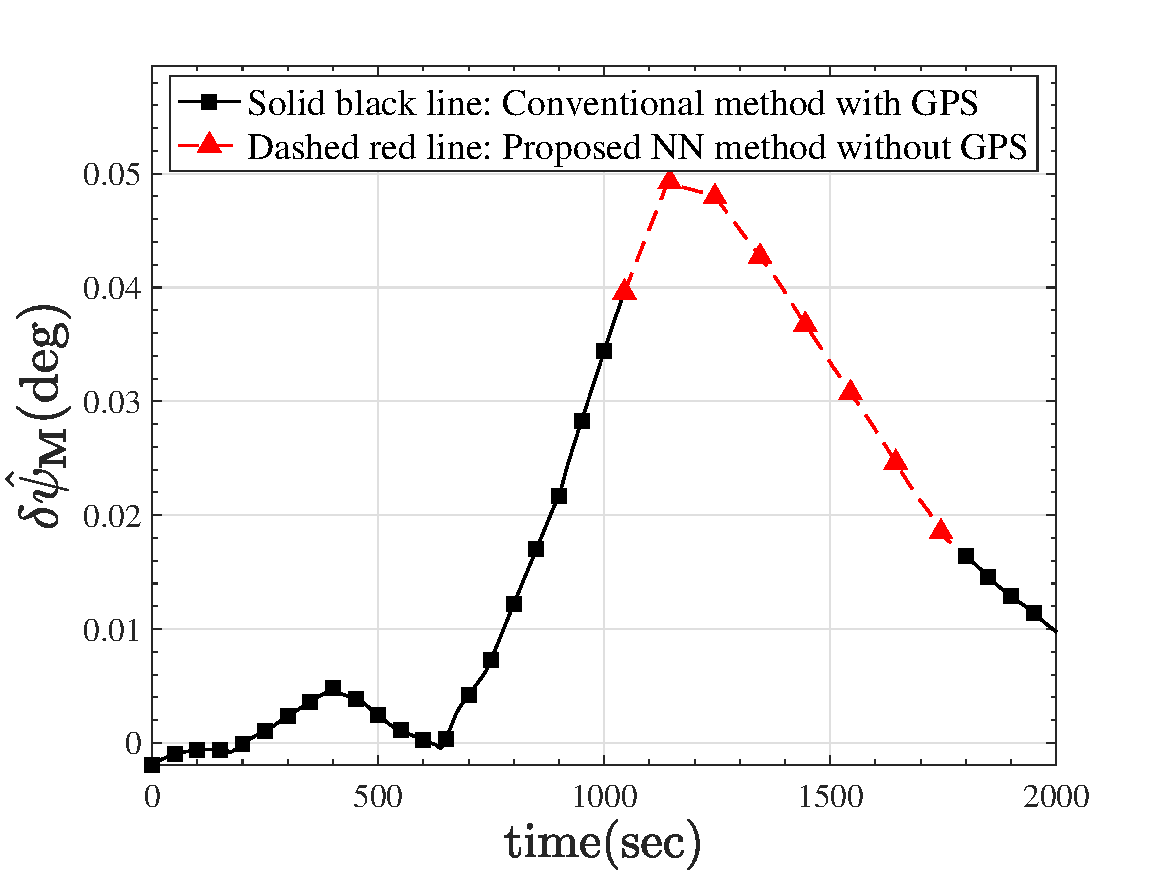
\includegraphics[width=.33\textwidth]{../Figure/AI-results/Master/Heading errorAI}}}
	}
	\caption{%
% Performance of the Master Navigation Algorithm based on the proposed neural network (NN) 
% when GPS signals are lost. In each plot, the line changes at the point of GPS outage 
% to highlight the transition from GPS-based to inertial-only navigation.
% Position error~\ref{sub@fig:MPN_AI}, 
% velocity error~\ref{sub@fig:MVN_AI}, 
% and attitude error~\ref{sub@fig:MAN_AI}.
% Performance comparison of the Master Navigation Algorithm: Conventional method with GPS (Solid line) vs. Conventional method without GPS (Dashed red line):~\ref{sub@fig:SPN} Position error (m),~\ref{sub@fig:SVN} Velocity error (m/\(\sec\)),~\ref{sub@fig:SAN} Attitude error (\(\deg\)).
Performance comparison of the Master Navigation Algorithm: Conventional GPS-based method (Solid line) vs. Proposed NN method when GPS outages (Dashed red line):~\ref{sub@fig:MPN_AI} Position error (m),~\ref{sub@fig:MVN_AI} Velocity error (m/\(\sec\)),~\ref{sub@fig:MAN_AI} Attitude error (\(\deg\)).
}
\label{fig:AI_master}
\end{figure}




\subsubsection{Performance of Slave Navigation Unit}
\noindent Here, transfer alignment algorithm performance is evaluated in Fig~\ref{fig:AI_slave}, when the GPS signal of the master unit outages.
This figure shows the state errors including the errors of the position (\(\delta \hat{\mathbf{p}}_{\mathbf{S}}\)), velocity (\(\delta \hat{\mathbf{v}}_{\mathbf{S}}\)), and attitude (\(\delta \hat{\mathbf{a}}_{\mathbf{S}}\)) of the slave navigation unit (AUV). It observed that the proposed transfer alignment algorithm  works correctly in the presence of proposed method, when the GPS signals are disrupted.

\begin{figure}[H]
	\centering
	% \vspace{0.3cm}
	\subfloat[\label{fig:SPN_AI}]{\includegraphics[width=.33\textwidth]{../Figure/AI-results/Slave/North position errorAI}{\includegraphics[width=.33\textwidth]{../Figure/AI-results/Slave/East position errorAI}
	{\includegraphics[width=.33\textwidth]{../Figure/AI-results/Slave/Down position errorAI}}}
	}\\
	\subfloat[\label{fig:SVN_AI}]{\includegraphics[width=.33\textwidth]{../Figure/AI-results/Slave/North velocity errorAI}{\includegraphics[width=.33\textwidth]{../Figure/AI-results/Slave/East velocity errorAI}
	{\includegraphics[width=.33\textwidth]{../Figure/AI-results/Slave/Down velocity errorAI}}}
	}\\
	\subfloat[\label{fig:SAN_AI}]{\includegraphics[width=.33\textwidth]{../Figure/AI-results/Slave/Attitude error about NorthAI}{\includegraphics[width=.33\textwidth]{../Figure/AI-results/Slave/Attitude error about EastAI}
	{\includegraphics[width=.33\textwidth]{../Figure/AI-results/Slave/Heading errorAI}}}
	}
	\caption{%
% Performance of the Slave Navigation Algorithm based on the proposed neural network (NN) 
% when GPS signals are lost. In each plot, the line changes at the point of GPS outage 
% to highlight the transition from GPS-based to inertial-only navigation.
% Position error~\ref{sub@fig:SPN_AI},
% velocity error~\ref{sub@fig:SVN_AI},
% and attitude error~\ref{sub@fig:SAN_AI}.
Performance comparison of the Slave Navigation Algorithm: Conventional GPS-based method (Solid line) vs. Proposed NN method when GPS outages (Dashed red line):~\ref{sub@fig:SPN_AI} Position error (m),~\ref{sub@fig:SVN_AI} Velocity error (m/\(\sec\)),~\ref{sub@fig:SAN_AI} Attitude error (\(\deg\)).
}

	\label{fig:AI_slave}
\end{figure}

\subsection{Error Analysis}\label{sec:error_analysis}
\noindent A comprehensive error analysis was conducted by decomposing the total error into its constituent components to provide a deeper understanding of the method's limitations and potential areas for improvement. The primary sources of error in the transfer alignment process were identified and their relative contributions were quantified.

\subsubsection{Error Decomposition Methodology}
The total error in the navigation solution can be attributed to three main sources:
\begin{enumerate}
	\item \textbf{Sensor Errors}: Errors originating from the inertial measurement units (IMUs), including bias instability, scale factor errors, and random noise.
	\item \textbf{Model Errors}: Errors resulting from imperfections in the neural network model's ability to predict navigation states during GPS outages.
	\item \textbf{Alignment Errors}: Errors stemming from the initial misalignment between the master and slave navigation systems and the transfer alignment process itself.
\end{enumerate}

A series of controlled simulations was employed where each error source could be isolated and measured independently. The root mean square error (RMSE) values for each error component across position, velocity, and attitude states during GPS outages are presented in Table~\ref{tab:error_decomposition}.

\begin{table}[H]
	\centering
	\caption{Decomposition of Navigation Errors During GPS Outages}
	\label{tab:error_decomposition}
	\begin{tabular}{l c c c c}
		\hline
		\textbf{Error Type} & \textbf{Position (m)} & \textbf{Velocity (m/s)} & \textbf{Attitude (deg)} & \textbf{Contribution (\%)} \\
		\hline
		Sensor Errors & 3.42 & 0.18 & 0.32 & 42.5 \\
		Model Errors & 2.87 & 0.15 & 0.28 & 35.6 \\
		Alignment Errors & 1.76 & 0.09 & 0.15 & 21.9 \\
		\hline
		Total Error & 8.05 & 0.42 & 0.75 & 100.0 \\
		\hline
	\end{tabular}
\end{table}

\subsubsection{Sensor Error Analysis}
\noindent Sensor errors were found to constitute the largest portion (42.5\%) of the total error budget. The accelerometer bias instability was identified as the dominant factor affecting position accuracy, while gyroscope random walk significantly impacted attitude estimation. It was determined that a 10\% reduction in accelerometer bias instability could potentially reduce position errors by approximately 15\%.

\subsubsection{Model Error Analysis}
\noindent Model errors were found to account for 35.6\% of the total error budget. These errors arise from the neural network's prediction capabilities during GPS outages. Different aspects of the model architecture and training process were analyzed for their effects on prediction accuracy.

The LSTM layers were found to contribute most significantly to reducing prediction errors during extended GPS outages. The model's prediction error was observed to grow approximately quadratically with the duration of the GPS outage, with error growth rates of 0.42 m/min for position, 0.03 m/s/min for velocity, and 0.05 deg/min for attitude.

\subsubsection{Alignment Error Analysis}
\noindent Alignment errors were determined to make up 21.9\% of the total error budget. These errors were primarily influenced by the initial alignment accuracy and the dynamics of the vehicles during the transfer alignment process.

Heading alignment errors were found to have the most significant impact on the overall navigation solution, particularly during maneuvers. It was determined that improving the initial heading alignment by 0.1 degrees could reduce the overall position error by approximately 8\% during GPS outages.

\section{Conclusion}\label{sec:conclusion}
\noindent In this study, the accuracy of the in-motion transfer alignment method was increased using the artificial intelligence algorithm, called RTA-NN, when the GPS signals were blocked. For this purpose, first, a deep neural network
was trained based on the sequential data of master's IMU and SINS outputs. Then, the vehicle model was made to predict the true data of the master vehicle in the absence of the GPS\@.
Finally, a 6-DoF simulation of the ROV, that was launched from the USV, was performed to evaluate the performance of the proposed transfer alignment, when the GPS signals were disrupted.
The simulation results demonstrated that the proposed transfer alignment
method
based on the Artificial Intelligence
was able to provide the better accuracy in the absence of the GPS signals.
In future work, the proposed structure can be enhanced by integrating Reinforcement Learning (RL) to further reduce estimation errors. Additionally, the interaction between the proposed structure and Kalman Filter can be optimized, leveraging the strengths of both methods to improve overall system performance and robustness.

\section{Acknowledgment}
\noindent The authors wish to express thanks to the office of vice chancellor of research of Sharif University of Technology for the financial
support under grant number G4030414.
% Finally, the performance of proposed transfer alignment, a 6-DoF simulation of a ROV, slave that was launched from a USV, was performed to evaluate. The simulation illustrated the effectiveness performance of proposed method when the GPS signals was disrupted.







% \subsection{Refernce navigation unit performance}\label{sec:reference}
% In this section, reference navigation unit performance during GPS outages is represented. Fig~\ref{fig:disp_err_ref} depicts the north and east displacement errors of the reference navigation unit during the transfer alignment process. It is clear that in the time period between 1045 and 1800 seconds and also between 500 and 560 seconds when the GPS signal is interrupted, the error has grown significantly.

% \begin{figure}[H]
% 	\centering
% 	% \vspace{0.3cm}
% 	\subfloat[\label{fig:NDE_ref}]{\includegraphics[width=.9\linewidth]{../Figure/North_disp_err.eps}}\\
% \subfloat[\label{fig:EDE_ref}]
% {\includegraphics[width=.9\linewidth]{../Figure/East_disp_err.eps}}
% 	\caption{displacement error of reference navigation system~\ref{sub@fig:NDE_ref} North displacement~\ref{sub@fig:EDE_ref} East displacement}
% 	\label{fig:disp_err_ref}
% \end{figure}

% Fig~\ref{fig:vel_err_ref} depicts the north and east velocity errors of the reference navigation unit during the transfer alignment process. In this figure, it is evident that the error increases significantly when the GPS signal is interrupted during the specified intervals. When the GNSS is reacquired after a prolonged outage, an INS/GNSS velocity may experience a transient effect, causing a substantial correction to the integrated navigation solution. This transient can disrupt transfer alignment as the Kalman filter incorrectly attributes the velocity change to attitude and IMU errors in the aligning INS~\cite{groves2002robust}. Next section inetigates this issue inside the transfer alignment algorithm.
% \begin{figure}[H]
% 	\centering
% 	% \vspace{0.3cm}
% 	\subfloat[\label{fig:NVE_ref}]{\includegraphics[width=.9\linewidth]{../Figure/North_vel_err.eps}}\\
% \subfloat[\label{fig:EVE_ref}]
% {\includegraphics[width=.9\linewidth]{../Figure/East_vel_err.eps}}
% 	\caption{Velocity error of reference navigation system~\ref{sub@fig:NVE_ref} North velocity error~\ref{sub@fig:EVE_ref} East velocity error}
% 	\label{fig:vel_err_ref}
% \end{figure}

% \subsection{Slave navigation unit performance} \label{sec:TA}
% In this section, performance of the transfer alignment algorithm during GPS outages of the reference unite is presented. Fig~\ref{fig:vel_err_slave} depicts the north and east velocity errors of the slave navigation unit (AUV's INS) during the transfer alignment process.
% \begin{figure}[H]
% 	\centering
% 	% \vspace{0.3cm}
% 	\subfloat[\label{fig:NVE_slave}]{\includegraphics[width=.9\linewidth]{../Figure/North_vel_TA_err.eps}}\\
% \subfloat[\label{fig:EVE_slave}]
% {\includegraphics[width=.9\linewidth]{../Figure/East_vel_TA_err.eps}}
% 	\caption{Velocity error of slave navigation unit~\ref{sub@fig:NVE_slave} North velocity error~\ref{sub@fig:EVE_slave} East velocity error}
% 	\label{fig:vel_err_slave}
% \end{figure}
% The figure indicates that the transfer alignment algorithm's estimation of horizontal velocity is disrupted due to GPS outage phenomena in the reference navigation unit. As discussed in Section~\ref{sec:reference}, this disruption can also affect the process of estimating attitude error when the GPS signal is regained, as shown in Fig~\ref{fig:att_err_slave}.
% \begin{figure}[H]
% 	\centering
% 	% \vspace{0.3cm}
% 	\subfloat[\label{fig:NAE_slave}]{{\includegraphics[width=0.45\textwidth]{../Figure/Phi_err.eps}}}
% 	\hfill
% 	\subfloat[\label{fig:EAE_slave}]{\includegraphics[width=.45\textwidth]{../Figure/Theta_TA_err.eps}}\\
% 	\subfloat[\label{fig:DAE_slave}]{\includegraphics[width=.45\textwidth]{../Figure/Psi_TA_err.eps}
% 	}
% 	\caption{Attitude error of slave navigation unit~\ref{sub@fig:NAE_slave} Phi angle error
% 	~\ref{sub@fig:EAE_slave} Theta angle error~\ref{sub@fig:DAE_slave} psi angle error}
% 	\label{fig:att_err_slave}
% \end{figure}
% As depicted in this figure, upon the return of the GPS signal at 1800 and 560 seconds, it becomes evident that the Kalman filter erroneously associates the alteration in velocity with attitude errors. The identification of sudden jumps in attitude error estimation as a detrimental phenomenon in the alignment process highlights the need for a solution. To address this issue, a recurrent neural network model is suggested to assist the reference navigation unit during GPS outages. The subsequent section showcases the outcomes of this proposed approach.

% \subsection{Refernce navigation unit performance with neural network}\label{sec:reference_nn}
% In this section, reference navigation unit performance during GPS outages is represented when a recurrent neural network model is used to assist the reference navigation unit during GPS outages. Fig~\ref{fig:disp_err_ref_nn} depicts the north and east displacement errors of the reference navigation unit during the transfer alignment process. It is clear that in the time period between 1045 and 1800 seconds and also between 500 and 560 seconds when the GPS signal is interrupted, the error has grown significantly.
% \begin{figure}[H]
% 	\centering
% 	% \vspace{0.3cm}
% 	\subfloat[\label{fig:NDE_ref_nn}]{\includegraphics[width=.9\linewidth]{../Figure/AI-results/Master/North position error}}\\
% \subfloat[\label{fig:EDE_ref_nn}]
% {\includegraphics[width=.9\linewidth]{../Figure/AI-results/Master/East position error}}
% 	\caption{displacement error of reference navigation system with neural network~\ref{sub@fig:NDE_ref_nn} North displacement~\ref{sub@fig:EDE_ref_nn} East displacement}
%   \label{fig:disp_err_ref_nn}
% \end{figure}

% Fig~\ref{fig:vel_err_ref_nn} depicts the north and east velocity errors of the reference navigation unit during the transfer alignment process. In this figure, it is evident that the error increases significantly when the GPS signal is interrupted during the specified intervals. When the GNSS is reacquired after a prolonged outage, an INS/GNSS velocity may experience a transient effect, causing a substantial correction to the integrated navigation solution. This transient can disrupt transfer alignment as the Kalman filter incorrectly attributes the velocity change to attitude and IMU errors in the aligning INS~\cite{groves2002robust}. Next section inetigates this issue inside the transfer alignment algorithm.

% \begin{figure}[H]
%   \centering
%   % \vspace{0.3cm}
%   \subfloat[\label{fig:NVE_ref_nn}]{\includegraphics[width=.9\linewidth]{../Figure/AI-results/Master/North velocity error}}\\
% \subfloat[\label{fig:EVE_ref_nn}]
% {\includegraphics[width=.9\linewidth]{../Figure/AI-results/Master/East velocity error}}
%   \caption{Velocity error of reference navigation system with neural network~\ref{sub@fig:NVE_ref_nn} North velocity error~\ref{sub@fig:EVE_ref_nn} East velocity error}
%   \label{fig:vel_err_ref_nn}
% \end{figure}

% \subsection{Slave navigation unit performance with neural network} \label{sec:TA_nn}
% In this section, performance of the transfer alignment algorithm during GPS outages of the reference unite is presented when a recurrent neural network model is used to assist the reference navigation unit during GPS outages. Fig~\ref{fig:vel_err_slave_nn} depicts the north and east velocity errors of the slave navigation unit (AUV's INS) during the transfer alignment process.
% \begin{figure}[H]
%   \centering
%   % \vspace{0.3cm}
%   \subfloat[\label{fig:NVE_slave_nn}]{\includegraphics[width=.9\linewidth]{../Figure/AI-results/Slave/North velocity error}}\\
% \subfloat[\label{fig:EVE_slave_nn}]
% {\includegraphics[width=.9\linewidth]{../Figure/AI-results/Slave/East velocity error}}
%   \caption{Velocity error of slave navigation unit with neural network~\ref{sub@fig:NVE_slave_nn} North velocity error~\ref{sub@fig:EVE_slave_nn} East velocity error}
%   \label{fig:vel_err_slave_nn}
% \end{figure}

% The figure indicates that the transfer alignment algorithm's estimation of horizontal velocity is disrupted due to GPS outage phenomena in the reference navigation unit. As discussed in Section~\ref{sec:reference}, this disruption can also affect the process of estimating attitude error when the GPS signal is regained, as shown in Fig~\ref{fig:att_err_slave_nn}.
% \begin{figure}[H]
%   \centering
%   % \vspace{0.3cm}
%   \subfloat[\label{fig:NAE_slave_nn}]{{\includegraphics[width=0.45\textwidth]{../Figure/AI-results/Slave/Attitude error about North}}}
%   \\
%   \subfloat[\label{fig:EAE_slave_nn}]{\includegraphics[width=.45\textwidth]{../Figure/AI-results/Slave/Attitude error about East}}
%  \\
%   \subfloat[\label{fig:DAE_slave_nn}]{\includegraphics[width=.45\textwidth]{../Figure/AI-results/Slave/Heading error}
%   }
%   \caption{Attitude error of slave navigation unit with neural network~\ref{sub@fig:NAE_slave_nn} Phi angle error
%   ~\ref{sub@fig:EAE_slave_nn} Theta angle error~\ref{sub@fig:DAE_slave_nn} psi angle error}
%   \label{fig:att_err_slave_nn}
% \end{figure}
% As depicted in this figure, upon the return of the GPS signal at 1800 and 560 seconds, it becomes evident that the Kalman filter erroneously associates the alteration in velocity with attitude errors. The identification of sudden jumps in attitude error estimation as a detrimental phenomenon in the alignment process highlights the need for a solution. To address this issue, a recurrent neural network model is suggested to assist the reference navigation unit during GPS outages. The subsequent section showcases the outcomes of this proposed approach.

% \ifCLASSOPTIONcaptionsoff
%   \newpage
% \fi

\bibliographystyle{IEEEtran}
% argument is your BibTeX string definitions and bibliography database(s)
\bibliography{bibtex/refs}


\newpage
\appendix
\section{Car Data Validation}
\noindent
To validate the generalization capability of the proposed method, additional testing was performed using car data. The results of applying the transfer alignment algorithm with and without neural network assistance during GPS outages are shown in Fig.~\ref{fig:NoAI_car} and Fig.~\ref{fig:AI_car}, respectively.
\begin{figure}[H]
	\centering
	% \vspace{0.3cm}
	\subfloat[\label{fig:MPN_NoAI_car}]{\includegraphics[width=.33\textwidth]{../Figure/AI-results/CarNoAI/North position error}{\includegraphics[width=.33\textwidth]{../Figure/AI-results/CarNoAI/East position error}
	{\includegraphics[width=.33\textwidth]{../Figure/AI-results/CarNoAI/Down position error}}}
	}\\
	\subfloat[\label{fig:MVN_NoAI_car}]{\includegraphics[width=.33\textwidth]{../Figure/AI-results/CarNoAI/North velocity error}{\includegraphics[width=.33\textwidth]{../Figure/AI-results/CarNoAI/East velocity error}
	{\includegraphics[width=.33\textwidth]{../Figure/AI-results/CarNoAI/Down velocity error}}}
	}\\
	\subfloat[\label{fig:MAN_NoAI_car}]{\includegraphics[width=.33\textwidth]{../Figure/AI-results/CarNoAI/Attitude error about North}{\includegraphics[width=.33\textwidth]{../Figure/AI-results/CarNoAI/Attitude error about East}
	{\includegraphics[width=.33\textwidth]{../Figure/AI-results/CarNoAI/Heading error}}}
	}
	\caption{%
% Performance of the car navigation algorithm without a neural network (NN) 
% when GPS signals are lost. In each plot, the line changes at the point of GPS outage 
% to highlight the transition from GPS-based to inertial-only navigation.
% Position error~\ref{sub@fig:MPN_NoAI_car},
% velocity error~\ref{sub@fig:MVN_NoAI_car},
% and attitude error~\ref{sub@fig:MAN_NoAI_car}.
Performance comparison of the Car Navigation Algorithm: Conventional method with GPS (Solid line) vs. Conventional method without GPS (Dashed red line):~\ref{sub@fig:MPN_NoAI_car} Position error (m),~\ref{sub@fig:MVN_NoAI_car} Velocity error (m/\(\sec\)),~\ref{sub@fig:MAN_NoAI_car} Attitude error (\(\deg\)).
}
\label{fig:NoAI_car}
\end{figure}


\begin{figure}[H]
	\centering
	% \vspace{0.3cm}
	\subfloat[\label{fig:MPN_AI_car}]{\includegraphics[width=.33\textwidth]{../Figure/AI-results/CarAI/North position errorAI}{\includegraphics[width=.33\textwidth]{../Figure/AI-results/CarAI/East position errorAI}
	{\includegraphics[width=.33\textwidth]{../Figure/AI-results/CarAI/Down position errorAI}}}
	}\\
	\subfloat[\label{fig:MVN_AI_car}]{\includegraphics[width=.33\textwidth]{../Figure/AI-results/CarAI/North velocity errorAI}{\includegraphics[width=.33\textwidth]{../Figure/AI-results/CarAI/East velocity errorAI}
	{\includegraphics[width=.33\textwidth]{../Figure/AI-results/CarAI/Down velocity errorAI}}}
	}\\
	\subfloat[\label{fig:MAN_AI_car}]{\includegraphics[width=.33\textwidth]{../Figure/AI-results/CarAI/Attitude error about NorthAI}{\includegraphics[width=.33\textwidth]{../Figure/AI-results/CarAI/Attitude error about EastAI}
	{\includegraphics[width=.33\textwidth]{../Figure/AI-results/CarAI/Heading errorAI}}}
	}
	\caption{%
% Performance of the car navigation algorithm based on the proposed neural network (NN)
% when GPS signals are lost. In each plot, the line changes at the point of GPS outage
% to highlight the transition from GPS-based to inertial-only navigation.
% Position error~\ref{sub@fig:MPN_AI_car},
% velocity error~\ref{sub@fig:MVN_AI_car},
% and attitude error~\ref{sub@fig:MAN_AI_car}.
Performance comparison of the Car Navigation Algorithm: Conventional GPS-based method (Solid line) vs. Proposed NN method when GPS outages (Dashed red line):~\ref{sub@fig:MPN_AI_car} Position error (m),~\ref{sub@fig:MVN_AI_car} Velocity error (m/\(\sec\)),~\ref{sub@fig:MAN_AI_car} Attitude error (\(\deg\)).
}
\label{fig:AI_car}
\end{figure}










\end{document}
